\documentclass[11pt,a4paper,twoside]{book}
% We load package by package and set package relevant parameters.
% Topics are summarized later
%%%%%%%%%%%%%%%%%%%%%%%%%%%%%%%%%%%%%%%%%%%%%%%%%%%%%%%%%%%%%%%%%%%%%%%%
% helping packages
\usepackage{ifthen}
\usepackage{calc}

% added by mike
\usepackage{booktabs}  % needed for table?
\usepackage{tabularx}  % needed for table?
\usepackage{tikz}     % needed for plot of MA and DAG (methods Experiment 1)
\usepackage{algorithmicx} % needed for algorithms
\usepackage{algorithm} % needed for algorithms



\usepackage[T1]{fontenc}       % provides fonts having  accented characters 
\usepackage[latin1]{inputenc}  % allows the user to input accented characters directly from the keyboard

%%%%%%%%%%%%%%%%%%%%%%%%%%%%%%%%%%%%%%%%%%%%%%%%%%%%%%%%%%%%%%%%%%%%%%%%

\renewcommand{\baselinestretch}{1.2}
\renewcommand{\textfraction}{0}%0.2     % placement of figures
\renewcommand{\topfraction}{1}%.3
\renewcommand{\bottomfraction}{1}%.3
\renewcommand{\floatpagefraction}{1}%.3
\setcounter{bottomnumber}{3}%1

\textwidth6.3in
\textheight9.7in
\topmargin-45pt
\oddsidemargin-.15in
\evensidemargin.15in
\headsep30pt
\headheight15pt
%\footskip20pt


%%%%%%%%%%%%%%%%%%%%%%%%%%%%%%%%%%%%%%%%%%%%%%%%%%%%%%%%%%%%%%%%%%%%%%%%

\usepackage[dvipsnames]{xcolor}
\definecolor{fgcolor}{rgb}{0.345, 0.345, 0.345}
\definecolor{shadecolor}{rgb}{.97, .97, .97}
\definecolor{messagecolor}{rgb}{0, 0, 0}
\definecolor{warningcolor}{rgb}{1, 0, 1}
\definecolor{errorcolor}{rgb}{1, 0, 0}
\definecolor{DarkBlue}{rgb}{0,0,0.5451}
\definecolor{DarkGreen}{rgb}{0,0.39216,0}
\definecolor{LightYellow}{rgb}{1,1,.8}
\definecolor{orange}{rgb}{.9,0.3445,0}



%%%%%%%%%%%%%%%%%%%%%%%%%%%%%%%%%%%%%%%%%%%%%%%%%%%%%%%%%%%%%%%%%%%%%%%%
\usepackage{afterpage}
\usepackage{natbib}
\usepackage{upquote}

\usepackage[english]{babel}

%%%%%%%%%%%%%%%%%%%%%%%%%%%%%%%%%%%%%%%%%%%%%%%%%%%%%%%%%%%%%%%%%%%%%%%%%%%%%%%
%% maxwidth is the original width if it is less than linewidth
%% otherwise use linewidth (to make sure the graphics do not exceed the margin)
\makeatletter
\def\maxwidth{ %
  \ifdim\Gin@nat@width>\linewidth
    \linewidth
  \else
    \Gin@nat@width
  \fi
}
\makeatother

%%%%%%%%%%%%%%%%%%%%%%%%%%%%%%%%%%%%%%%%%%%%%%%%%%%%%%%%%%%%%%%%%%%%%%%%%%%%%%%%%%%%%%%%%%%%%%%%%%%%%%%%%%%%
% from fancyvrb
\usepackage{fancyhdr}
\usepackage{fancyvrb}
\DefineVerbatimEnvironment{Rcode}{Verbatim}{xleftmargin=2em,fontshape=sl,formatcom=\color{DarkGreen}}
\fvset{listparameters={\setlength{\topsep}{0pt}}}

%%%%%%%%%%%%%%%%%%%%%%%%%%%%%%%%%%%%%%%%%%%%%%%%%%%%%%%%%%%%%%%%%%%%%%%%%%%%%%%%%%%%%%%%%%%%%%%%%%%%%%%%%%%%%
\usepackage{float}
\usepackage{graphicx}
\usepackage[margin=2em,labelfont=bf]{caption}


%%%%%%%%%%%%%%%%%%%%%%%%%%%%%%%%%%%%%%%%%%%%%%%%%%%%%%%%%%%%%%%%%%%%%%%%
\usepackage[pdftex,plainpages=false,pdfpagelabels,pagebackref=true,colorlinks=true,pdfpagemode=UseOutlines]{hyperref}


%%%%%%%%%%%%%%%%%%%%%%%%%%%%%%%%%%%%%%%%%%%%%%%%%%%%%%%%%%%%%%%%%%%%%%%%
% now math stuff and other details...
\usepackage{amsmath,amsthm,amssymb}

\newtheorem{pro}{Property}[chapter]
\theoremstyle{definition}
\newtheorem{des}{Definition}[chapter]
\newtheorem{bsp}{Example}[chapter]
\newtheorem{rem}{Remark}[chapter]

% % for pseudocode
\usepackage{algorithm}
\usepackage{algpseudocode}

\newcommand*\widebar[1]{%
  \vbox{%
    \hrule height 0.5pt%     % Line above with certain width
    \kern0.5ex%             % Distance between line and content
    \hbox{%
      \kern-0.1em%           % Distance between content and left side of box, negative values for lines shorter than content
      \ifmmode#1\else\ensuremath{#1}\fi%  % The content, typeset in dependence of mode
      \kern-0.1em%      % Distance between content and left side of box, negative values for lines shorter than content
    }% end of hbox
  }% end of vbox
}
\def\ds{\displaystyle}

\newcommand{\rr}[1]{{\ttfamily\slshape\color{DarkGreen} #1}}

\makeatletter


% clever trick to circumvent potential redefines after loading packages:
% \providecommand{\something}{}  % if it does not exist, it creates it.
%      has same syntax as \newcommand
% \renewcommand{\something}{....}
% TUGboat 29(2)


\makeatletter
%umdefinierung exisitierender befehle
\let\oldH\H
\let\oldL\L
\let\oldO\H
\let\oldS\S
\let\olda\a
\let\oldb\b
\let\oldc\c
\let\oldd\d
\let\oldk\k
\let\oldv\v
\let\oldl\l
\let\oldt\t
\let\oldu\u
\let\oldIJ\IJ
\let\oldP\P
\let\P\relax
\let\oldnorm\|

%\DefineVerbatimEnvironment{CodeInput}{Verbatim}{fontshape=sl}
%\DefineVerbatimEnvironment{CodeOutput}{Verbatim}{}

% some classical environments, up-right, with chapter numbering.
\theoremstyle{definition}
\newtheorem{definition}{Definition}[chapter]
\newtheorem{example}{Example}[chapter]
\newtheorem{remark}{Remark}[chapter]
\newtheorem{theorem}{Theorem}[chapter]



\renewcommand{\|}{|\!|}         % closer norm
\newcommand{\T}{{}^{\top}}
\newcommand\code[1]{{\tt#1}}

%%% renamed to customalgo because package is used above
\newcounter{algo}
\newenvironment{customalgo}{%
  \begin{list}{
      (\arabic{algo})
    }{
      \usecounter{algo}
    }%
}{
  \end{list}
}


% \newcounter{algo}
% \newenvironment{algorithm}{%
%   \begin{list}{
%       (\arabic{algo})
%     }{
%       \usecounter{algo}
%     }%
% }{
%   \end{list}
% }

% some text abbreviation
\newcommand{\GLS}{\text{GLS}}
\newcommand{\RR}{\text{RR}}
\newcommand{\OR}{\text{OR}}
\newcommand{\WLS}{\text{WLS}}
\newcommand{\MLE}{\text{MLE}}
\newcommand{\OLS}{\text{OLS}}
\newcommand{\MAE}{\text{MAE}}
\newcommand{\MAD}{\text{MAD}}
\newcommand{\RMSE}{\text{RMSE}}

\newcommand{\ii}{\text{\i}}

\newcommand{\Bin}{\cB\mathit{\!i\!n}}
\newcommand{\Beta}{\cB\mathit{\!e\!t\!a}}
\newcommand{\Pois}{\cP\mathit{\!o\!i\!s\!s\!o\!n}}
\newcommand{\Exp}{\cE\mathit{\!x\!p}}


\DeclareMathOperator*{\argmin}{argmin}
\DeclareMathOperator*{\argmax}{argmax}
\DeclareMathOperator{\diag}{diag}
\DeclareMathOperator{\diam}{diam}
\DeclareMathOperator{\card}{card}
\DeclareMathOperator{\cov}{Cov}                   
\DeclareMathOperator{\corr}{Corr}                 
\DeclareMathOperator{\var}{Var}                   
\DeclareMathOperator{\trace}{tr}                  
\DeclareMathOperator{\E}{E}                       
\DeclareMathOperator{\P}{P}                       
\DeclareMathOperator{\pred}{p}
\DeclareMathOperator{\vect}{vec}                  
\DeclareMathOperator{\vech}{vech}                 
\DeclareMathOperator{\rank}{rank}                 
\DeclareMathOperator{\e}{e}                       
%\DeclareMathOperator{\cv}{CV}                     
\DeclareMathOperator{\GCV}{GCV}                     
\DeclareMathOperator{\CV}{CV}                     
\DeclareMathOperator{\BLUP}{BLUP}                 
\DeclareMathOperator{\MSE}{MSE}                   
\DeclareMathOperator{\MS}{MS}                   
\DeclareMathOperator{\df}{df}                   
\DeclareMathOperator{\bias}{bias}                   
\DeclareMathOperator{\eig}{eig}                   
\DeclareMathOperator{\Prec}{Prec}
\DeclareMathOperator{\mode}{mode}
\renewcommand{\SS}{\text{SS}}
\renewcommand{\d}{\mathsf{\,d}}

\def\arctanh{\qopname\relax o{arctanh}}  % as in amsopn
\newcommand{\bigo}{\cO}
\newcommand{\lito}{\text{\scriptsize{$\cO$}}}
\newcommand{\cdfPhi}{\itPhi}
\newcommand{\ml}{_\text{ML}}

\newcommand*{\stack@relbin}[3][]{%
  \mathop{#3}\limits
  \toks@{#1}%
  \edef\reserved@a{\the\toks@}%
  \ifx\reserved@a\@empty\else_{#1}\fi
  \toks@{#2}%
  \edef\reserved@a{\the\toks@}%
  \ifx\reserved@a\@empty\else^{#2}\fi
  \egroup
}%
\renewcommand*{\stackrel}{\mathrel\bgroup\stack@relbin}
\newcommand*{\stackbin}{\mathbin\bgroup\stack@relbin}
\newcommand{\simiid}{\stackrel[]{\text{iid}}{\sim}}

% Kalligraphischer Schriftsatz
\newcommand{\cA}{{\cal{A}}}
\newcommand{\cB}{{\cal{B}}} 
\newcommand{\cC}{{\cal{C}}}
\newcommand{\cD}{{\cal{D}}} 
\newcommand{\cE}{{\cal{E}}}
\newcommand{\cF}{{\cal{F}}}
\newcommand{\cG}{{\cal{G}}}
\newcommand{\cH}{{\cal{H}}}
\newcommand{\cI}{{\cal{I}}}
\newcommand{\cJ}{{\cal{J}}}
\newcommand{\cK}{{\cal{K}}}
\newcommand{\cL}{{\cal{L}}}
\newcommand{\cM}{{\cal{M}}} 
\newcommand{\cN}{{\cal{N}}}
\newcommand{\cO}{{\cal{O}}} 
\newcommand{\cP}{{\cal{P}}}
\newcommand{\cQ}{{\cal{Q}}} 
\newcommand{\cR}{{\cal{R}}} 
\newcommand{\cS}{{\cal{S}}} 
\newcommand{\cT}{{\cal{T}}}
\newcommand{\cU}{{\cal{U}}}
\newcommand{\cV}{{\cal{V}}}
\newcommand{\cW}{{\cal{W}}}
\newcommand{\cX}{{\cal{X}}} 
\newcommand{\cY}{{\cal{Y}}}
\newcommand{\cZ}{{\cal{Z}}} 


\newcommand{\IA}{{\mathbb{A}}}
\newcommand{\IB}{{\mathbb{B}}}
\newcommand{\IC}{{\mathbb{C}}}
\newcommand{\ID}{{\mathbb{D}}}
\newcommand{\IE}{{\mathbb{E}}}
\newcommand{\IF}{{\mathbb{F}}}
\newcommand{\IG}{{\mathbb{G}}}
\newcommand{\IH}{{\mathbb{H}}}
\newcommand{\II}{{\mathbb{I}}}
%\newcommand{\IJ}{{\mathbb{J}}}
\newcommand{\IK}{{\mathbb{K}}}
\newcommand{\IL}{{\mathbb{L}}}
\newcommand{\IM}{{\mathbb{M}}}
\newcommand{\IN}{{\mathbb{N}}}
\newcommand{\IO}{{\mathbb{O}}}
\newcommand{\IP}{{\mathbb{P}}}
\newcommand{\IQ}{{\mathbb{Q}}}
\newcommand{\IR}{{\mathbb{R}}}
\newcommand{\IS}{{\mathbb{S}}}
\newcommand{\IT}{{\mathbb{T}}}
\newcommand{\IU}{{\mathbb{U}}}
\newcommand{\IV}{{\mathbb{V}}}
\newcommand{\IW}{{\mathbb{W}}}
\newcommand{\IX}{{\mathbb{X}}}
\newcommand{\IY}{{\mathbb{Y}}}
\newcommand{\IZ}{{\mathbb{Z}}}


% fette griechische kleinbuchstaben
\newcommand{\balpha}{{\boldsymbol{\alpha}}}
\newcommand{\bbeta}{{\boldsymbol{\beta}}}
\newcommand{\bgamma}{{\boldsymbol{\gamma}}}
\newcommand{\bdelta}{{\boldsymbol{\delta}}}
\newcommand{\blambda}{{\boldsymbol{\lambda}}}
\newcommand{\bepsilon}{{\boldsymbol{\epsilon}}}
\newcommand{\bvarepsilon}{{\boldsymbol{\varepsilon}}}
\newcommand{\bzeta}{{\boldsymbol{\zeta}}}
\newcommand{\bfeta}{{\boldsymbol{\eta}}}  %  <----- exception !
\newcommand{\btheta}{{\boldsymbol{\theta}}{}}
\newcommand{\bvartheta}{{\boldsymbol{\vartheta}}}
\newcommand{\biota}{{\boldsymbol{\iota}}}
\newcommand{\bkappa}{{\boldsymbol{\kappa}}}
\newcommand{\bmu}{{\boldsymbol{\mu}}}
\newcommand{\bnu}{{\boldsymbol{\nu}}}
\newcommand{\bxi}{{\boldsymbol{\xi}}}
\newcommand{\bpi}{{\boldsymbol{\pi}}}
\newcommand{\bvarpi}{{\boldsymbol{\varpi}}}
\newcommand{\brho}{{\boldsymbol{\rho}}}
\newcommand{\bvarrhoi}{{\boldsymbol{\varrho}}}
\newcommand{\bsigma}{{\boldsymbol{\sigma}}}
\newcommand{\bvarsigma}{{\boldsymbol{\varsigma}}}
\newcommand{\btau}{{\boldsymbol{\tau}}}
\newcommand{\bvartau}{{\boldsymbol{\vartau}}}
\newcommand{\bupsilon}{{\boldsymbol{\upsilon}}}
\newcommand{\bphi}{{\boldsymbol{\phi}}}
\newcommand{\bvarphi}{{\boldsymbol{\varphi}}}
\newcommand{\bchi}{{\boldsymbol{\chi}}}
\newcommand{\bpsi}{{\boldsymbol{\psi}}}
\newcommand{\bomega}{{\boldsymbol{\omega}}}


% fette griechische grossbuchstaben
\newcommand{\bGamma}{{\boldsymbol{\Gamma}}}
\newcommand{\bDelta}{{\boldsymbol{\Delta}}}
\newcommand{\bTheta}{{\boldsymbol{\Theta}}}
\newcommand{\bLambda}{{\boldsymbol{\Lambda}}{}}
\newcommand{\bXi}{{\boldsymbol{\Xi}}}
\newcommand{\bPi}{{\boldsymbol{\Pi}}}
\newcommand{\bSigma}{{\boldsymbol{\Sigma}}{}}
\newcommand{\bUpsilon}{{\boldsymbol{\Upsilon}}{}}
\newcommand{\bPhi}{{\boldsymbol{\Phi}}}
\newcommand{\bPsi}{{\boldsymbol{\Psi}}}
\newcommand{\bOmega}{{\boldsymbol{\Omega}}}

% italics griechische grossbuchstaben
\newcommand{\itGamma}{{\mathit{\Gamma}}}
\newcommand{\itDelta}{{\mathit{\Delta}}}
\newcommand{\itTheta}{{\mathit{\Theta}}}
\newcommand{\itLambda}{{\mathit{\Lambda}}}
\newcommand{\itXi}{{\mathit{\Xi}}}
\newcommand{\itPi}{{\mathit{\Pi}}}
\newcommand{\itSigma}{{\mathit{\Sigma}}}
\newcommand{\itUpsilon}{{\mathit{\Upsilon}}}
\newcommand{\itPhi}{{\mathit{\Phi}}}
\newcommand{\itPsi}{{\mathit{\Psi}}}
\newcommand{\itOmega}{{\mathit{\Omega}}}



\newcommand{\A}{{\mathbf{A}}}
\newcommand{\B}{{\mathbf{B}}}
\newcommand{\C}{{\mathbf{C}}}
\newcommand{\D}{{\mathbf{D}}}
\newcommand{\bfE}{{\mathbf{E}}}    % \E: expectation
\newcommand{\F}{{\mathbf{F}}}
\newcommand{\G}{{\mathbf{G}}}
\renewcommand{\H}{{\mathbf{H}}}
\newcommand{\I}{{\mathbf{I}}}
\newcommand{\J}{{\mathbf{J}}}
\newcommand{\K}{{\mathbf{K}}}
\renewcommand{\L}{{\mathbf{L}}}
\newcommand{\bfM}{{\mathbf{M}}}
\newcommand{\N}{{\mathbf{N}}}
\renewcommand{\O}{{\mathbf{O}}}
\newcommand{\bfP}{{\mathbf{P}}}  % \P : probability
\newcommand{\Q}{{\mathbf{Q}}}
\newcommand{\bfR}{{\mathbf{R}}}
\renewcommand{\S}{{\mathbf{S}}}
\newcommand{\bfT}{{\mathbf{T}}} % \T transpose
\newcommand{\U}{{\mathbf{U}}}
\newcommand{\V}{{\mathbf{V}}}
\newcommand{\W}{{\mathbf{W}}}
\newcommand{\X}{{\mathbf{X}}}
\newcommand{\Y}{{\mathbf{Y}}}
\newcommand{\Z}{{\mathbf{Z}}}


\newcommand{\0}{{\mathbf{0}}}
\newcommand{\1}{{\mathbf{1}}}
\newcommand{\2}{{\mathbf{2}}}
\newcommand{\3}{{\mathbf{3}}}
\newcommand{\4}{{\mathbf{4}}}
\newcommand{\5}{{\mathbf{5}}}
\newcommand{\6}{{\mathbf{6}}}
\newcommand{\7}{{\mathbf{7}}}
\newcommand{\8}{{\mathbf{8}}}
\newcommand{\9}{{\mathbf{9}}}

\renewcommand{\a}{{\textbf{\textit{a}}}}
\renewcommand{\b}{{\textbf{\textit{b}}}}
\renewcommand{\c}{{\textbf{\textit{c}}}}
\newcommand{\bfd}{{\textbf{\textit{d}}}}  % \d  'dx'
\newcommand{\bfe}{{\textbf{\textit{e}}}}  % \e  l'exponentiel
\newcommand{\f}{{\textbf{\textit{f}}}}
\newcommand{\g}{{\textbf{\textit{g}}}}
\newcommand{\h}{{\textbf{\textit{h}}}}
\newcommand{\bfi}{{\textbf{\textit{i}}}}%\i  complex i, sans 'dot'
\newcommand{\bfj}{{\textbf{\textit{j}}}}
\renewcommand{\l}{{\textbf{\textit{l}}}}
\renewcommand{\k}{{\textbf{\textit{k}}}}
\newcommand{\m}{{\textbf{\textit{m}}}}
\newcommand{\bfn}{{\textbf{\textit{n}}}}
\newcommand{\bfo}{{\textbf{\textit{o}}}}
\newcommand{\p}{{\textbf{\textit{p}}}}
\newcommand{\q}{{\textbf{\textit{q}}}}
\renewcommand{\r}{{\textbf{\textit{r}}}}
\newcommand{\s}{{\textbf{\textit{s}}}}
\renewcommand{\t}{{\textbf{\textit{t}}}}
\newcommand{\bfu}{{\textbf{\textit{u}}}} %\u used in references
\renewcommand{\v}{{\textbf{\textit{v}}}}
\newcommand{\w}{{\textbf{\textit{w}}}}
\newcommand{\x}{{\textbf{\textit{x}}}}
\newcommand{\y}{{\textbf{\textit{y}}}}
\newcommand{\z}{{\textbf{\textit{z}}}}




\ifcsname hlkwd\endcsname%    ... command '#1' exists ...%
\else%  ... command '#1' does not exist ...%

\def\maxwidth{ %
  \ifdim\Gin@nat@width>\linewidth
    \linewidth
  \else
    \Gin@nat@width
  \fi
}

\definecolor{fgcolor}{rgb}{0.345, 0.345, 0.345}
\newcommand{\hlnum}[1]{\textcolor[rgb]{0.686,0.059,0.569}{#1}}%
\newcommand{\hlstr}[1]{\textcolor[rgb]{0.192,0.494,0.8}{#1}}%
\newcommand{\hlcom}[1]{\textcolor[rgb]{0.678,0.584,0.686}{\textit{#1}}}%
\newcommand{\hlopt}[1]{\textcolor[rgb]{0,0,0}{#1}}%
\newcommand{\hlstd}[1]{\textcolor[rgb]{0.345,0.345,0.345}{#1}}%
\newcommand{\hlkwa}[1]{\textcolor[rgb]{0.161,0.373,0.58}{\textbf{#1}}}%
\newcommand{\hlkwb}[1]{\textcolor[rgb]{0.69,0.353,0.396}{#1}}%
\newcommand{\hlkwc}[1]{\textcolor[rgb]{0.333,0.667,0.333}{#1}}%
\newcommand{\hlkwd}[1]{\textcolor[rgb]{0.737,0.353,0.396}{\textbf{#1}}}%

\usepackage{framed}
\newenvironment{kframe}{%
 \def\at@end@of@kframe{}%
 \ifinner\ifhmode%
  \def\at@end@of@kframe{\end{minipage}}%
  \begin{minipage}{\columnwidth}%
 \fi\fi%
 \def\FrameCommand##1{\hskip\@totalleftmargin \hskip-\fboxsep
 \colorbox{shadecolor}{##1}\hskip-\fboxsep
     % There is no \\@totalrightmargin, so:
     \hskip-\linewidth \hskip-\@totalleftmargin \hskip\columnwidth}%
 \MakeFramed {\advance\hsize-\width
   \@totalleftmargin\z@ \linewidth\hsize
   \@setminipage}}%
 {\par\unskip\endMakeFramed%
 \at@end@of@kframe}
\renewenvironment{kframe}{%
 \def\at@end@of@kframe{}%
 \ifinner\ifhmode%
  \def\at@end@of@kframe{\end{minipage}}%
  \begin{minipage}{\columnwidth}%
 \fi\fi%
 \def\FrameCommand##1{\hskip\@totalleftmargin \hskip-0\fboxsep
 \colorbox{shadecolor}{##1}\hskip-0\fboxsep
     % There is no \\@totalrightmargin, so:
     \hskip-\linewidth \hskip-\@totalleftmargin \hskip\columnwidth}%
 \MakeFramed {\advance\hsize-\width
   \@totalleftmargin\z@ \linewidth\hsize
   \@setminipage}}%
 {\par\unskip\endMakeFramed%
 \at@end@of@kframe}


\definecolor{shadecolor}{rgb}{.97, .97, .97}
\definecolor{messagecolor}{rgb}{0, 0, 0}
\definecolor{warningcolor}{rgb}{1, 0, 1}
\definecolor{errorcolor}{rgb}{1, 0, 0}
%\newenvironment{knitrout}{}{} % an empty environment to be redefined in TeX
\newenvironment{knitrout}{\setlength{\topsep}{0mm}\setlength{\fboxsep}{4mm}}{} 

\usepackage{alltt}
\IfFileExists{upquote.sty}{\usepackage{upquote}}{}

  \fi%

\makeatother
   % packages, layout and standard macros

\setcounter{secnumdepth}{3} % to show numbering for subsubsections


\begin{document}
\renewcommand\familydefault{\sfdefault} 
\pagenumbering{Alph}


\thispagestyle{empty}
\renewcommand{\baselinestretch}{1.5}\normalfont
\begin{center}
\setlength{\parindent}{0cm}
\bf\Large% 


Causal Modeling with Neural Networks \\
and Individualized Treatment Effect Estimation 

% Functional Modeling with Neural Causal Models \\
% and Personalized Treatment Effect Estimation 

% Modeling Functional Relationships in Causal Graphs \\
% and Estimating Individualized Interventions: \\
% Neural Causal Models (TRAM-DAGs) and \\
% Conditional Average Treatment Effects

\normalfont

% Neural Causal Models with TRAM-DAGs: \\
% A framework for modelling causal effects in a flexible and \\
% interpretable way and for making subsequent causal queries.\\


\hrulefill

\vspace*{4cm}

\large
Master Thesis in Biostatistics (STA495) % or choose the next one
% Master Thesis in Mathematics (MAT491) 
\vspace*{12mm}

by

\vspace*{12mm}

Mike Kr{\"a}henb{\"u}hl\\
\small Matriculation number: 18-652-149\\
\normalfont
\vspace*{4cm}

supervised by

\vspace*{1cm}

Prof. Dr. Beate Sick, University of Zurich \& ZHAW \\
Prof. Dr. Oliver D{\"u}rr, HTWG Konstanz
\vfill

Zurich, July 2025
\end{center}
\renewcommand\familydefault{\rmdefault}%
\renewcommand{\baselinestretch}{1.0}\rm 
\setcounter{page}{0}
\newpage
\vspace*{12cm}~\thispagestyle{empty}\pagenumbering{Roman}
\newpage


\graphicspath{{./figure/}}
\DeclareGraphicsExtensions{.pdf,.png}
\setcounter{tocdepth}{1}

\thispagestyle{empty}
\begin{center}
%

	\vspace*{6cm}{\bfseries\Huge
	Causal Modeling with Neural Networks \\ [5mm]
and \\ [5mm]
Individualized Treatment Effect Estimation \\ [5mm]
	}
	
	% Functional Modeling with Neural Causal Models and Personalized Treatment Effect Estimation 
	% Modeling Functional Relationships in Causal Graphs and Estimating Individualized Interventions:\\[5mm]
	% Neural Causal Models (TRAM-DAGs) and Conditional Average Treatment Effects
	
  % \vspace*{6cm}{\bfseries\Huge
  % Neural Causal Models with TRAM-DAGs:\\[5mm]
  % Applied on real-world data \\[5mm]
  % and used for ITE estimation.
  % }

  \vfill
  \rm

  \LARGE
  Mike Kr{\"a}henb{\"u}hl\\[12mm]
  
  \normalsize
  Version \today
\end{center}
\newpage
\thispagestyle{empty}~
\newpage
\pagenumbering{roman}

\thispagestyle{plain}\markboth{Contents}{Contents}
\tableofcontents
\setkeys{Gin}{width=.8\textwidth}

\chapter*{Preface}
\addtocontents{toc}{\protect \vspace*{13.mm}}
\addcontentsline{toc}{chapter}{\bfseries{Preface}}
\thispagestyle{plain}\markboth{Preface}{Preface}



This thesis marks the final part of my Master of Science in Biostatistics at the University of Zurich. I wanted to work on a topic where I could apply my interest and deepen my knowledge in machine learning, especially in relation to causal questions.

The TRAM-DAG framework \citep{sick2025}, developed by my supervisors Prof. Dr. Beate Sick and Prof. Dr. Oliver D{\"u}rr, provided a perfect opportunity to do so. Our initial aim was to apply it to real-world data and potentially include semi-structured data. However, due to some surprising findings by \citet{chen2025}, our focus shifted towards the increasingly important topic of individualized treatment effect (ITE) estimation. Towards the end, we then bridged ITE estimation with the TRAM-DAG framework.

I want to thank my supervisors and all the people I had the chance to work and study with, as well as everyone who supported me on this journey.

% In the introduction, our aim is to give a summary of key concepts in causal inference and causal models. We also motivate the need for methods that allow drawing causal conclusions from observational data and introduce the proposed framework of TRAM-DAGs \citep{sick2025} as a tool that can be used for this purpose. We also want to highlight the importance of estimation of personalized treatment effects. \\ 
% 
% In the methods section, we give a detailed description of the TRAM-DAG framework, how it works, and for what kinds of causal queries the model can be used. Although individualized treatment effect (ITE) estimation is not a typical observational data problem, we also discuss important considerations and how TRAM-DAGs and other models can be applied in this context. \\ 
% 
% Then, we persent results of simulation studies that show the capabilities of TRAM-DAGs, the analysis of potential limitations in ITE estimation, and the TRAM-DAG applied for ITE estimation. Additionally, we perform ITE estimation on the International Stroke Trial (IST) with different causal ML methods including TRAM-DAGs.\\ 
% 
% In the final sections, we discuss the results and draw conclusions about the strengths and limitations of the framework and ITE esitimaiton in general, while also providing an outlook for future research. 


\bigskip

\begin{flushright}
  Mike Kr{\"a}henb{\"u}hl\\
  July 2025
\end{flushright}

\addtocontents{toc}{\protect \vspace*{10mm}}

\cleardoublepage



%%%%%%%%%%%%%%%%%%%%%%%%%%%%%%%%%%%%%%%%%%%%%%%%%%%%%%%%%%%%%%%%%%%%%% 


\chapter*{Abstract}
\addtocontents{toc}{\protect \vspace*{13.mm}}
\addcontentsline{toc}{chapter}{\bfseries{Abstract}}
\thispagestyle{plain}\markboth{Abstract}{Abstract}



This thesis explores TRAM-DAGs, a flexible neural network-based framework for modeling complex causal relationships in known directed acyclic graphs (DAGs), and investigates their use -- alongside other models -- for estimating individualized treatment effects (ITEs). TRAM-DAGs allow sampling from observational, interventional, and counterfactual distributions when the full DAG is known. 
% We applied TRAM-DAGs to both simulated data and a real-world randomized controlled trial, with a focus on individualized treatment effect (ITE) estimation.

We show how TRAM-DAGs can be used with continuous and ordinal or categorical predictor variables, investigate how variable scaling affects interpretability, and demonstrate how interactions between variables can be modeled. A key part of this work involved applying different causal machine learning models -- including TRAM-DAGs, logistic regression, and random forests -- to estimate ITEs on the International Stroke Trial (IST) dataset. In line with findings by \citet{chen2025}, none of the models produced ITE estimates that generalized to the test data.

To explore possible reasons for this poor performance, we conducted simulation experiments under varying conditions. These revealed that, while models must be well calibrated and overfitting should be avoided, this alone may not suffice to guarantee valid ITE estimates. Weak treatment-covariate interaction effects and especially unmeasured effect modifiers were found to be critical challenges. When such variables are unobserved, the ignorability assumption alone may not ensure unbiased estimation -- an issue also highlighted by \citet{vegetabile2021}. These factors may help explain the limited model performance observed in the IST dataset.

We also applied TRAM-DAGs in randomized and confounded simulation settings with relatively complex DAGs and found that, when the full DAG was observed and interaction effects were present, TRAM-DAGs accurately recovered causal relationships and provided unbiased ITE estimates for a continuous outcome.

While promising, our work has limitations. The simulation scenarios may not fully capture real-world complexity, and evaluating ITE estimates on real data remains challenging since ground truth is unknown. The neural network-based TRAM-DAGs require training time and rely on modeling assumptions -- e.g., regarding the scale of conditional effects -- when parameter interpretability is desired.

TRAM-DAGs offer a customizable modeling framework that enables the specification of both flexibility and interpretability, making them suitable for real-world causal inference tasks. Future work could apply TRAM-DAGs to more diverse datasets, including semi-structured data, and further investigate ITE estimation in the presence of unmeasured effect modifiers.


% This thesis investigates the use of TRAM-DAGs \citep{sick2025} as a flexible approach for estimating structural equations in known directed acyclic graphs (DAGs). TRAM-DAGs offer several advantages: the model inherently knows when to control for covariates based on the DAG, is highly customizable in terms of flexibility and interpretability, and allows sampling from observational, interventional, and counterfactual distributions. We show how to incorporate ordinal predictors, model interactions, and examine how variable scaling affects interpretability.
% 
% A main focus was the estimation of individualized treatment effects (ITEs) using a variety of causal machine learning (ML) models. In simulation studies, we analyzed limitations in ITE estimation and found that unmeasured effect modifiers can severely impact estimation accuracy, and that the ignorability assumption alone may not ensure unbiased results -- a concern that has also been noted in prior research \citep{vegetabile2021}. The limitations found may also help explain the poor ITE estimation performance observed in the real-world application on the International Stroke Trial dataset \citep{chen2025}. We further demonstrated that TRAM-DAGs can be used for ITE estimation in relatively complex DAG structures, provided that the DAG is fully known and all variables are observed.
% 
% While promising, TRAM-DAGs require training time due to their reliance on neural networks and, when aiming for interpretability, certain assumptions about the model structure. Future work could explore applications to more real-world data, potentially including semi-structured inputs, and further investigate ITE estimation in the presence of unmeasured interactions.
% 
% This thesis contributes to the field of causal inference under observational data and to the estimation of personalized treatment effects using causal ML models.




% This thesis investigates the use of TRAM-DAGs as a flexible approach for estimating structural equations in known DAGs. TRAM-DAGs offer several advantages: the model knows when to adjust based on the DAG, avoids incorrect covariate adjustment, and allows sampling from observational, interventional, and counterfactual distributions. Their ability to combine interpretability with flexibility makes them well suited for practical use.
% We show how to incorporate ordinal predictors, model interactions, and how variable scaling affects interpretability. A main focus was the estimation of individualized treatment effects (ITEs), using a variety of causal machine learning (ML) models.
% In simulation studies, we analyzed limitations in ITE estimation where we found that However, we also found that unmeasured effect modifiers can severely impact ITE estimation, and that the ignorability assumption alone may not ensure unbiased results. We demonstrated that TRAM-DAGs can also be applied for ITE estimation in relatively complex DAG structures, when the DAG is fully known and all variables are observed.
% 
% The found limitations may also reflected reasons for poor ITE estimation performance in the real-world application on the International Stroke Trial.
% 
% While promising, TRAM-DAGs rely on neural networks and require training time and assumptions about model structure. Future work could apply them to more real-world data, possibly including semi-structured inputs, and further investigate ITE estimation with unmeasured interactions.
% 
% This thesis contributes to the field of causal inference under observational data and towards personalized treatment effect estimation using causal machine learning models.

\bigskip

\noindent\textbf{Keywords:} TRAM-DAGs, neural causal model, individualized treatment effect, structural causal model, counterfactuals, transformation model, observational data, heterogeneous treatment effect, conditional average treatment effect




\addtocontents{toc}{\protect \vspace*{10mm}}

\cleardoublepage

%%%%%%%%%%%%%%%%%%%%%%%%%%%%%%%%%%%%%%%%%%%%%%%%%%%%%%%%%%%%%%%%%%%%%% 

\pagenumbering{arabic}


%%%%%%%%%%%%%%%%%%%%%%%%%%%%%%%%%%%%%%%%%%%%%%%%%%%%%%%%%%%%%%%%%%%%%% 
%%%%%%%%%%%%%%%%%%%%%%%%%%%%%%%%%%%%%%%%%%%%%%%%%%%%%%%%%%%%%%%%%%%%%%

% LaTeX file for Chapter 01



%  possible title: Causal inference for non-randomized data and heterogeneous treatment effect estimation


\chapter{Introduction}

\section{Motivation}

% Why, what and how\dots

The most important questions in research are mostly not associational, but causal \citep{pearl2009}. They concern the effects of interventions -- such as the impact of a treatment -- or seek explanations for observed outcomes, such as identifying which disease caused certain symptoms. They also include hypothetical scenarios; for example: what would the gross domestic product have been if interest rates had increased by 25 instead of 75 basis points? Answering such questions requires causal reasoning and demands an understanding of the underlying data-generating process. Purely associational approaches are typically not sufficient to draw valid causal conclusions.

% https://ascpt.onlinelibrary.wiley.com/doi/epdf/10.1002/cpt.3159
% One of the main reasons for this is thatML methods are particularly good at learning about the status quofrom existing data to ultimately make outcome predictions thatare exactly in line with the current distribution of data character-istics, but usually not designed for tasks that involve the need toreason about interventions on the data generating distributionsleading to counterfactual scenarios,


The gold standard for estimating the causal effect of an intervention on an outcome is the randomized controlled trial (RCT) \citep{hariton2018}. In this prospective study design, participants are randomly assigned to either the treatment or control group. Randomization aims to eliminate the influence of potential confounding variables, ensuring that treatment groups are balanced with respect to baseline characteristics. This allows for an unbiased estimation of the causal effect. Despite their strengths, RCTs have several limitations. They are often expensive and time-consuming to plan and execute. Moreover, the results may not generalize well to the population of interest, as individuals who volunteer or are accepted for trials are not always representative of the target group. Another central limitation of RCTs is that in many scenarios they simply cannot be conducted due to ethical or practical reasons. For example, an RCT is only ethical in the case of clinical equipoise, which means that there is uncertainty about the superiority of one of the two treatment arms \citep{freedman1987}. It is not acceptable to treat one group with the assumed inferior treatment. The same is true for obviously harmful interventions, such as smoking or drinking alcohol. In these cases, it is not possible to conduct an RCT to estimate the causal effect of smoking on lung cancer. 

For these reasons, much of research aims to make causal inference from observational data, using non-experimental or quasi-experimental designs. Unlike RCTs, these settings do not involve randomization to treatment, which introduces challenges due to confounding. Methods for causal inference from observational data aim to correctly control for such confounders to enable valid causal conclusions. 

% Recently, \citet{sick2025} proposed the TRAM-DAGs framework, which estimates the functional form of causal relationships in a known causal graph based on observational or RCT data, and can then be used to make subsequent causal queries. In this thesis, we further analyze and apply this method.

% In the context of personalized medicine, it is therefore crucial to have an estimate of treatment effects at the individual level. 
An application where causal inference is of particular importance is the estimation of personalized treatment effects. RCTs typically estimate an average treatment effect (ATE) on a sample, which is the difference in mean outcomes between the treatment and the control groups \citep{nichols2007}. However, individual patients may respond differently to the treatment, depending on their unique characteristics. 
In personalized medicine, the estimate of treatment effects at the individual level is referred to as the individualized treatment effect (ITE) or conditional average treatment effect (CATE), while in business and marketing contexts, the term uplift modeling is often used \citep{gutierrez2017, zhao2020}. Such estimates are critical in settings where treatment responses vary significantly between individuals. For clinical decision-making, tailoring therapies to individual characteristics can lead to more effective and efficient care. The importance of estimating individual-level effects is not limited to medicine. It is also of high interest in marketing, where campaigns can be precisely targeted to maximize impact and minimize adverse responses. Consider, for instance, the decision of whether to send a push notification (treatment) to a customer. Some customers might be persuadables, who will respond positively only if treated. Others, in contrast, might have responded positively without the intervention but are negatively affected by receiving it -- for example, a customer who is reminded of a forgotten subscription and, as a result, decides to cancel it. In this context, identifying persuadables is valuable, while treating the latter may be counterproductive. This illustrates the need to understand treatment effects at a granular level to guide individualized decisions.
Various methods have been proposed to estimate individualized treatment effects, yet this task remains challenging. The fundamental problem is that only one of the two potential outcomes can ever be observed for any given individual \citep{holland1986}, making the estimation of treatment effects inherently more difficult than standard predictive modeling.

% \citep{gutierrez2017, zhao2020}

\medskip

These two motivations -- causal inference from observational data and the estimation of individualized treatment effects — form the focus of this thesis. We build on existing methods to address both challenges. The next sections provide an overview of key concepts and methods, and lay out the specific research questions we aim to answer.





\section{Key concepts of causal inference}

% Causal relationships can be represented by a directed acyclic graph (DAG), as shown in Figure~\ref{fig:pearl_levels}(a). The variables, or nodes, are connected by directed edges, which represent causal dependencies.


% Visual examples of these levels are presented in Figure~\ref{fig:pearl_levels}(a)--(c). redundant, later i refer to it again
Questions in causal inference are typically classified into one of the three levels of Pearl's hierarchy of causation \citep{pearl_book2009}. Level 1 corresponds to observational queries, expressed as conditional probabilities $\text{P}(Y \mid X)$, which can be answered directly from the joint distribution $\text{P}(Y \cap X)$. Level 2 involves interventional queries, such as $\text{P}(Y \mid \text{do}(X = \alpha))$, which describe the probability when intervening on a variable $X$ and setting it to a particular value. Level 3 addresses counterfactual reasoning. These are hypothetical what-if questions that require reasoning about outcomes under alternative realities. For example, if a patient received a treatment and died, the factual outcome is death under the received treatment. The counterfactual would be the outcome that would have occurred had the patient received a different treatment.

 
% Some statisticians argue that counterfactuals -- being unobservable and untestable -- are of limited scientific value and may be regarded as metaphysical \citep{dawid2000}. Nevertheless, there are important practical questions that require the analysis of such counterfactuals.


% 
% % include image /img/pearl_levels.png
% \begin{figure}[H]
% \centering
% 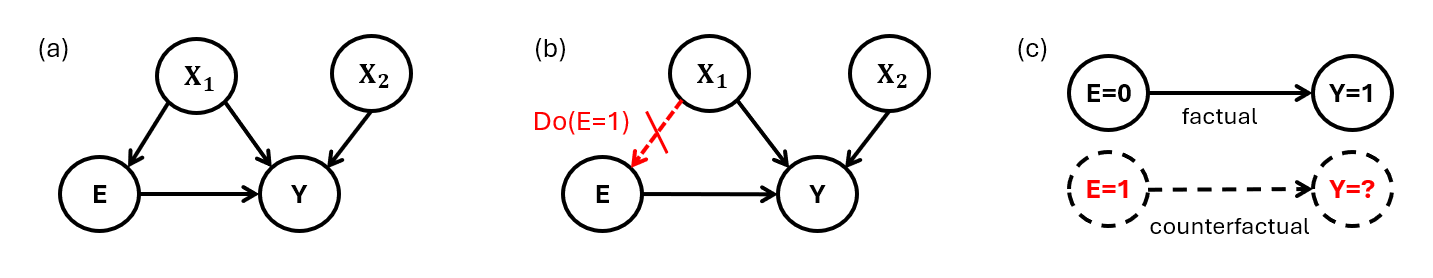
\includegraphics[width=1\textwidth]{img/pearl_levels.png}
% \caption{Illustration of the three levels of Pearl's hierarchy of causation. (a) Directed acyclic graph (DAG) for observational data. (b) DAG when making a do-intervention by fixing the variable $E$ at a certain value. (c) Observed factual outcome and the corresponding counterfactual query.}
% \label{fig:pearl_levels}
% \end{figure}
% 
% 
% To illustrate Pearl's three levels of causality, we consider a simplified example involving the exposure Exercise ($E$), the outcome Heart Disease ($Y$), the confounder Age ($X_1$) and the additional covariate Smoking ($X_2$). I assume that exercise reduces the risk of heart disease, but both variables are also influenced by age. Figure~\ref{fig:pearl_levels}(a)--(c) illustrates the corresponding scenarios.
% 
% 
% 
% 
% 
% \textbf{Level 1: Observational ("seeing"):}  
% We observe the joint distribution of variables without intervention.  
% Example: What is the probability of heart disease given that a person exercises?  
% \[
% P(Y = 1 \mid E = 1)
% \]
% This can be estimated directly from data by conditioning on $E = 1$ and computing the frequency of $Y = 1$. However, such an estimate does not account for confounding variables like age.
% 
% 
% 
% \textbf{Level 2: Interventional ("doing"):}  
% We consider the effect of actively intervening in the system.  
% Example: What is the probability of heart disease if everyone were made to exercise, regardless of age or smoking status?  
% \[
% P(Y = 1 \mid \text{do}(E = 1))
% \]
% Answering this requires assumptions about the underlying causal structure.
% 
% 
% 
% \textbf{Level 3: Counterfactual ("imagining"):}  
% We ask what would have happened under different circumstances -- that is, we imagine an alternative scenario for the same individual.  
% Example: For a person who does not exercise and has heart disease, would they still have had heart disease if they had exercised?  
% \[
% P(Y_{E=1} \mid E = 0, Y = 1)
% \]
% 
% Here, $Y_{E=1}$ represents the counterfactual outcome under positive exposure. Counterfactual queries cannot be answered from observational data alone; they require a structural framework that explicitly models the data-generating process. 


% With our new framework, we can answer all three types of questions, with a small exception for Counterfactuals in the non-continuous case.




Causal relationships can be represented by a directed acyclic graph (DAG), where the variables, or nodes, are connected by directed edges, which represent causal dependencies.

% the following all from pearl book p. 27
While DAGs capture the structure of these dependencies, structural causal models (SCMs) extend this representation by explicitly modeling the functional relationships between variables. A set of structural equations of the form $X_i = f_i(\text{pa}(X_i), Z_i), \quad i = 1, \dots, n$ defines an SCM \citep{pearl_book2009}. Here, $\text{pa}(X_i)$ denotes the direct causal parents of $X_i$, and $Z_i$ is an exogenous noise variable. These exogenous variables capture latent factors that influence $X_i$ but are not explicitly modeled. By convention, the $Z_i$ are assumed to be mutually independent. This assumption implies that the DAG includes all involved variables and causal connectivities. Any dependence between variables must be due to a direct or indirect path in the graph; otherwise, dependencies would show up in the noise terms, violating their independence \citep{pearl_book2009}.

Each function $f_i$ -- which may be nonlinear -- defines how the value of $X_i$ is generated from its parents and the corresponding noise term. A source node $X_j$ without any parents is modeled as $X_j = f_j(Z_j)$. Once all structural equations and noise variables are specified, the model is fully deterministic in the sense that each variable is a fixed function of its parents and its own exogenous noise. The randomness in the system arises entirely from these independent noise terms. This functional representation makes it possible to compute interventional distributions and evaluate counterfactual outcomes. These aspects are discussed in detail in Section~\ref{methods:sampling}.

In this thesis, we do not focus on discovering the underlying causal graph. Such a structure may be obtained through structure learning algorithms (see e.g., \citealp{zheng2018}) or determined from expert knowledge. Instead, we assume the graph is known and concentrate on estimating the functional form of the relationships between variables -- that is, the structural equations that define the SCM.

Various approaches exist for estimating the functions $f_i$ that constitute an SCM, depending on the assumptions made about the data and the model class.




% \[
% X_i = \beta_0 + \beta_1 X_{pa(x_i)} + Z_i
% \]
%
% \[
%   X \sim \mathcal{N}(\mu = pa(X)\beta,\,\sigma^{2})\,.
% \]


A simple approach to modeling the structural equations is linear regression, which assumes Gaussian error terms $Z_i$ and linear functional forms $f_i$. Classical statistical methods of this kind are typically well-defined, computationally efficient, and offer interpretable parameters. However, they rely on strong assumptions about the underlying data-generating mechanism -- such as linearity and homoscedasticity -- which often do not hold in practice. Violations of these assumptions can lead to biased or misleading results.

Alternatively, more flexible approaches based on tree-based ensemble models or neural networks have gained popularity for estimating structural equations. These models are capable of approximating complex, nonlinear relationships and capturing complicated interactions between variables with minimal bias. Their flexibility, however, often comes at the cost of reduced interpretability and, in some cases, limited applicability to non-continuous or mixed data types. \citet{poinsot2024} provided an overview of deep structural causal models and their use in counterfactual inference.

The TRAM-DAG framework proposed by \citet{sick2025} builds a bridge between these classical and neural-network-based modeling approaches, by combining interpretable transformation models with the flexibility of neural networks. At its core, the structural equations are modeled using transformation models \citep{hothorn2014}, a flexible class of distributional regression methods. These models were subsequently extended to deep transformation models (Deep TRAMs) by \citet{sick2020}, enabling the use of neural networks to estimate the parameters of the transformation function in a flexible and customizable way. In the TRAM-DAG framework, these deep TRAMs are applied according to a known causal graph, allowing the model to be fitted to observational data and used to answer causal queries across all three levels of Pearl's hierarchy. The framework is introduced in more detail in Section~\ref{sec:tram_dags}.





\section{Goals and contributions} \label{sec:goals_contributions}

The first part of this thesis focuses on the TRAM-DAG framework. In particular, we apply the model to DAGs of varying complexity, extend it from continuous to ordinal and categorical predictors, examine how variable scaling affects the interpretation of coefficients, and make use of different neural network configurations (e.g., activation functions, batch normalization, dropout). Most analyses are conducted on simulated data, where the underlying data-generating process is known, but the model is also applied to real-world data to demonstrate its practical utility.

The second focus of the thesis is the estimation of individualized treatment effects (ITEs). Recent work by \citet{chen2025} showed that most causal machine learning models trained on RCT data failed to generalize when evaluated out of sample. We replicate part of their study by applying various models they used, as well as TRAM-DAGs, to the same data and analyze whether we reach similar conclusions. We further investigate why ITE estimation may fail in such settings and under which conditions reliable estimates can be obtained. In addition, we demonstrate that TRAM-DAGs can be effectively used to estimate ITEs also in complex, non-randomized observational settings, provided the causal graph is known and fully observed. In doing so, we explore the potential of TRAM-DAGs as a framework for answering causal questions across different levels of Pearl's hierarchy.

\medskip

Formally, we aim to answer the following research questions in this thesis:

\begin{itemize}
    \item How can TRAM-DAGs be applied to estimate causal relationships across different scenarios, and subsequently be used to sample from observational, interventional, and counterfactual distributions? Using synthetic data, we demonstrate how the model can be applied and explain how to handle ordinal and categorical predictors, how variable scaling affects the interpretation of coefficients, and how interactions between variables can be modeled.

    
    \item Do we reach similar conclusions as \citet{chen2025} when applying their models, as well as TRAM-DAGs, to the International Stroke Trial (IST) dataset for ITE estimation? Specifically, we examine whether ITEs estimated on the training data fail to generalize to the test data.

    \item What factors contribute to the failure of ITE estimation in causal machine learning models, and under which conditions can reliable estimates be obtained? We investigate this by applying various models across simulated scenarios that differ in observed variables and treatment effect size.

    \item Can TRAM-DAGs provide unbiased estimates of ITEs when the causal graph is fully observed? We evaluate this in a complex simulation setting with a continuous outcome, comparing both randomized and confounded designs.
\end{itemize}




% 
% \begin{itemize}
%     \item How can TRAM-DAGs be applied under different scenarios such as ordinal predictors, scaled vs. raw variables or allowing for interactions between variables?
%     \item Do we obtain similar results when estimating ITEs on a real-world RCT dataset, as reported by \citet{chen2025}?
%     \item What are possible reasons for the failure of ITE estimation in some cases when causal machine learning models are validated out of sample?
%     \item How can TRAM-DAGs be used to estimate ITEs in both randomized controlled trials and observational settings involving confounding and mediating variables?
% \end{itemize}



With this work, we aim to contribute to the important and evolving field of causal inference in observational settings and to the challenging task of estimating individualized treatment effects.


%%%%%%%%%%%%%%%%%%%%%%%%%%%%%%%%%%%%%%%%%%%%%%%%%%%%%%%%%%%%%%%%%%%%%% 
%%%%%%%%%%%%%%%%%%%%%%%%%%%%%%%%%%%%%%%%%%%%%%%%%%%%%%%%%%%%%%%%%%%%%%



% LaTeX file for Chapter 02


\chapter{Methods} 

In this section I will explain the necessary background needed to understand the TRAM-DAGs. Once the framework of tram dags is explained, I will present how the experiments of the simulation, the application on real data and the ITE estimation are conducted.


The goal of TRAM-DAGs is to estimate the structural equations according to the causal order in a given DAG in a flexible and possibly still interpretable way in order to sample observational and interventional distributions and to make counterfactual statements. The estimation requires data and a DAG that describes the causal structure. It must be assumed that there are no hidden confounders. TRAM-DAGs estimate for each variable $X_i$ a transformation function $Z_i = h_i(X_i \mid pa(X_i))$, where $Z_i$ is the noise value and $pa(X_i)$ are the causal parents of $X_i$. The important part here is that we can rearrange this equation to $X_i = h_i^{-1}(Z_i \mid pa(x_i))$ to get to the structural equation. The transformation functions $h$ are monotonically increasing functions that are a representation of the conditional distribution of $X_i$ on a latent scale. They are based on the idea of transformation models as introduced by \citet{hothorn2014} but were extended to deep trams by \citet{sick2020}. In the following sections I review the most important ideas of these methods as they are the essential components of TRAM-DAGs.

\section{Transformation Models}


Transformation models are a flexible distributional regression method for various data types. They can be for example specified as ordinary linear regression, logistic regression or proportional odds logistic regression. But Transformation models further allow to model conditional outcome distributions that do not even need to belong to a known distribution family of distributions by model it in parts flexibly. This reduces the strength of the assumptions that have to be made.

The basic form of transformation models can be described by

\begin{equation}
F(y|\mathbf{x}) = F_Z(h(y \mid \mathbf{x})) =  F_Z(h_I(y) - \mathbf{x}^\top \boldsymbol{\beta})
\label{eq:transformation_model}
\end{equation}

, where $F(y|\mathbf{x})$ is the conditional cumulative distribution function of the outcome variable $Y$ given the predictors $\mathbf{x}$. $h(y \mid \mathbf{x})$ is a transformation function that maps the outcome variable $y$ onto the latent scale of $Z$. $F_Z$ is the cumulative distribution function of a latent variable $Z$, the so-called inverse-link function that maps $h(y \mid \mathbf{x})$ to probabilities. In this basic version, the transformation function can be split into an intercept part $h_I(y)$ and a linear shift part $\mathbf{x}^\top \boldsymbol{\beta}$, where the vector $\mathbf{x}$ are the predictors and $\boldsymbol{\beta}$ are the corresponding coefficients.

If the latent distribution $Z$ is chosen to be the standard logistic distribution, then the coefficient $\beta_i$ can be interpreted as log-odds ratios when increasing the predictor $x_i$ by one unit, holding all other predictors unchanged. This means that an increase of one unit in the predictor $x_i$ leads to an increase of the log-odds of the outcome $Y$ by $\boldsymbol{\beta}$. The additive shift of the transformation function means a linear shift on the latent scale (herer log-odds). The following transformation to probabilities by $F_Z$ potentially leads to a non-linear change in the conditional outcome distribution on the original scale. This means not only is the distribution shifted, also its shape can change to some degree based on the covariates. More details about the choice of the latent distribution and the interpretation of the coefficients are provided in the appendix XXX.


For a continuous outcome $Y$ the intercept $h_I$ is represented by a bernstein polynomial, which is a flexible and monotonically increasing function

\begin{equation}
h_I(y) = \frac{1}{M + 1} \sum_{k=0}^{M} \vartheta_k \, \text{B}_{k, M}(y)
\end{equation}

, where $\vartheta_k$ are the coefficients of the bernstein polynomial and $\text{B}_{k, M}(y)$ are the Bernstein basis polynomials. More details about the technical implementation of the bernstein polynomial in the context of TRAM-DAGs is given in the appendix XXX.

For a discrete outcome $Y$ the intercept $h_I$ is represented by cut-points, which are the thresholds that separate the different levels of the outcome. For example, for a binary outcome $Y$ there is one cut-point and for an ordinal outcome with $K$ levels there are $K-1$ cut-points. The transformation model is given by

\begin{equation}
P(Y \leq y_k \mid \mathbf{X} = \mathbf{x}) = F_Z(\vartheta_k + \mathbf{x}^\top \boldsymbol{\beta}), \quad k = 1, 2, \ldots, K - 1
\end{equation}


A visual representation for a continuous and discrete (ordinal) outcome is provided in Figure~\ref{fig:tram_cont_ord}.


% include image /img/tram_cont_ord.png
\begin{figure}[H]
\centering
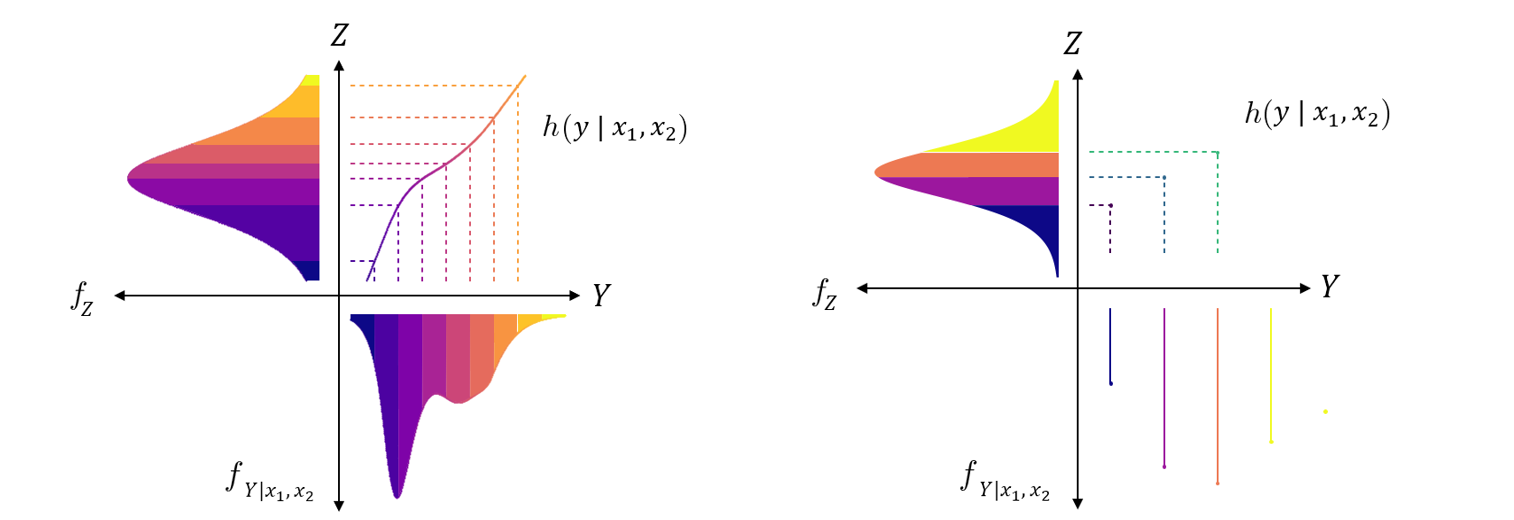
\includegraphics[width=1\textwidth]{img/tram_cont_ord.png}
\caption{\textbf{Left:} Example of a transformation model for a continuous outcome $Y$ with a smooth transformation function. \textbf{Right:} Example of a transformation model for an ordinal outcome $Y$ with 5 levels. The transformation function consists of cut-points that separate the probabilities for the levels of the outcome.
In both cases the latent distribution $Z$ is the standard logistic and the predictors $\mathbf{x}$ induce a linear (vertical) shift of the transformation function.}
\label{fig:tram_cont_ord}
\end{figure}


To estimate the parameters $\boldsymbol{\beta}$ and $\boldsymbol{\vartheta}$ the negative log likelihood (NLL) is minimized. The NLL is defined as

\begin{equation}
\text{NLL} = - \frac{1}{n} \sum_{i=1}^{n} l_i(\boldsymbol{\beta}, \boldsymbol{\vartheta} ) = - \frac{1}{n} \sum_{i=1}^{n} \log (f_{Y \mid \mathbf{X} = \mathbf{x}}(y_i))
\label{eq:nll_tram}
\end{equation}

where $l_i(\boldsymbol{\beta}, \boldsymbol{\vartheta})$ is the log-likelihood of the $i$-th observation,  $l_i(\boldsymbol{\beta}, \boldsymbol{\vartheta}) = f_{Y \mid \mathbf{X} = \mathbf{x}}(y_i)$ is the conditional density function of the outcome variable $Y$ given the predictors $\mathbf{x}$ under the current parameterization. I provide the full derivation in the appendix xxx.


For the remainder of this thesis, I rely on the idea of these transformation models to model the conditional distribution functions represented by the transformation functions of the respective variables. The standard logistic distribution is used as $F_Z$, which results in a logistic transformation model.


\section{Deep TRAMs} \label{sec:deep_trams}

The transformation models as discussed before were extended to deep TRAMs using a modular neural network \citep{sick2020}. The goal is to get a parametrized transformation function of the form \ref{eq:deep_tram.}.Each part, the intercept $h_I(X_i)$, the linear shift $\mathbf{x}_L^\top \boldsymbol{\beta}_L$ and the complex shift $f_C(\mathbf{x}_C)$ are assembled by the outputs of the individual neural networks. The user can specify the level of complexity the parents $pa(X_i)$ have on the transformaiton funciton. Figure \ref{fig:deep_tram} illustrates the case for a SI-LS-CS model.

\begin{equation}
h(y \mid \mathbf{x}_L, \mathbf{x}_C ) = h_I(y) + \mathbf{x}_L^\top \boldsymbol{\beta}_L + f_C(\mathbf{x}_C)
\label{eq:deep_tram}
\end{equation}



\begin{figure}[H]
\centering
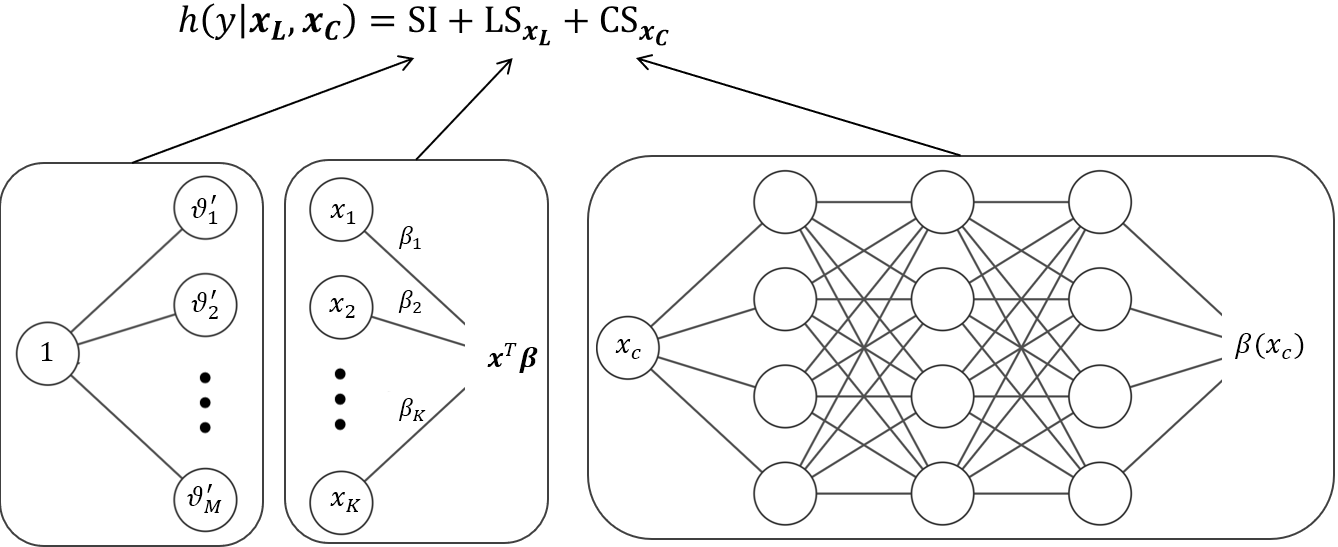
\includegraphics[width=0.9\textwidth]{img/deep_tram.png}
\caption{Modular deep transformation model. The transformation function $h(y \mid \mathbf{x})$ is constructed by the outputs of three neural networks.}
\label{fig:deep_tram}
\end{figure}

\textbf{Intercept } the shape of the transformation function at the baseline configuration $\mathbf{x}_L^\top \boldsymbol{\beta}_L = 0$ and $f_C(\mathbf{x}_C)=0$ is determined by the intercept $h_I(y)$. For a continuous outcome the intercept is represented by a smooth bernstein polynomial and in the discrete case by cut-points. In either case the parameters $\vartheta$ are obtained as output nodes of the neural network. A simple intercept (SI) is the case where the parameters $\vartheta$ do not depend on the any explanatory variables. The neural network thereby only takes a constant as input and directly outputs the parameters $\vartheta$. To make the intercept more flexible, the intercept can also depend on the explanatory variables. In this case the complex intercept (CI) models the intercept $\vartheta(x)$ by taking the predictors $x$ as input to a neural network with some hidden layers. This allows the intercept to change with the value of the predictors. Depending on the assumptions, predictors can be used in the complex intercept, or only a subset of them. A detailed explanation of the construction of the bernstein polynomial is given in appendix XXX.

\textbf{Linear shift } If the predictors should have a linear effect on the transformation function, it can be modelled by a linear shift (LS). For this part the neural network without hidden layers and without biases takes the linear predictors $pa(X_i)$ as input and generates a single output node with a linear activation function. This results in the linear combination $\mathbf{x}_L^\top \boldsymbol{\beta}_L$ and it induces a linear vertical shift of the transformation function. The weights $\boldsymbol{\beta}_L$ are the interpretable coefficients of the linear shift. For the logistic transformation model, they are interpreted as log-odds-ratios.
The interpretation is further described in the appendix XX.

\textbf{Complex shift } If the transformation function should be allowed to be shifted vertically in a non-linear manner, a complex shift (CS) can be applied. The predictor variables are inputed in a (deep) neural network with at least one hidden layer and a single output node with $f_C(X_C)$ is obtained. With a complex shift, also interactions between predictor variables can be captured.


\textbf{Level of complexity } One practical feature of these modular deep TRAMs is that one can specify, which predictors should have a linear or complex shift effect on the transformation function or that predictors are even allowed to deterimine the shape of the transformation function by a complex intercept. \citet{herzog2023} predicted the ordinal functional outcome three months after stroke by using semi-structured data that included tabular predictors and images. The two data modalities can be included in a single deep TRAM by modeling the part of the images with a CNN.

The estimated distribution function is invariant with respect to the choice of the inverse-link function $F_Z$ (scale of latent distribution) in an unconditional \citep{hothorn2018} or fully flexible (CI) setting. However, as soon as restrictions are placed on the influence of the predictors (LS, CS), this leads to assumptions about the scale of the dependency. Which latent distribution should be chosen depends on following factors: (i) the intended complexity of the model, (ii) the assumptions about the data generating process, (iii) the conventional, widely used, scale of interpretation for the specific problem. If the coefficients $\beta$ in the linear shift term should be interpreted as log odds ratios, then the standard logistic distribution is appropriate. For log hazard ratios it would be the minimum extreme value distribution. There exist plenty of other alternatives.

(The optimal scale could be found by comparing the likelihoods of the model under different latent distributions. )



\textbf{Parameter estimation } The parameters of the neural networks are learned by  minimizing the negative log-likelihood (NLL) of the conditional deep TRAM. The learning process is started with a random parameter configuration and the outputs of the neural networks are used to assemble the NLL of the transformation model. The NLL is then iteratively minimized by adjusting the parameters by the Adam optimizer \citep{kingma2015} until they eventually converge to the optimum state. Additionally, methods to prevent overfitting --- such as dropout, early stopping, or batch normalization --- can be applied. These techniques are particularly important in more complex networks to ensure that the model generalizes well to out-of-sample data. In the hidden layers, non-linear activation functions such as ReLU or sigmoid are applied.




\section{TRAM-DAGs}



In TRAM-DAGs these deep transformation models are applied in a causal setting. We assume a pre-specified DAG which defines the causal dependence. Then we estimate the distribution of each node by a transformation model that is conditional on its parents. Figrue \ref{fig:tram_dag} illustrates the basic idea of a TRAM-DAG where a DAG with 3 variables, without hidden confounder, is assumed to be known. The arrows in the DAG indicate the causal dependencies between the variables. The transformation models are constructed by a modular neural network. The assumed influence from the parent variables has to be specified as SI, LS or CS. In this example, $X_1$ is a continuous source node that acts as parent of $X_2$ and $X_3$. For a source node the transformation function only consists of a simple intercept (SI). $X_2$ is also continuous and its transformation function can be shifted additively (LS) by the value of $X_1$. $X_3$ is an ordinal variable with 4 levels and its transformation function depends on the values of $X_1$ (LS) and $X_2$ (CS). The cut-points $h(x_3 \mid x_1, x_2)$ represent the cumulative probabilities on the log-odds scale of the first 3 levels of $X_3$, where the probability of the last level $K=4$ is the complement of the previous levels $k_{1-3}$.

% include image /img/tram_dag.png
\begin{figure}[H]
\centering
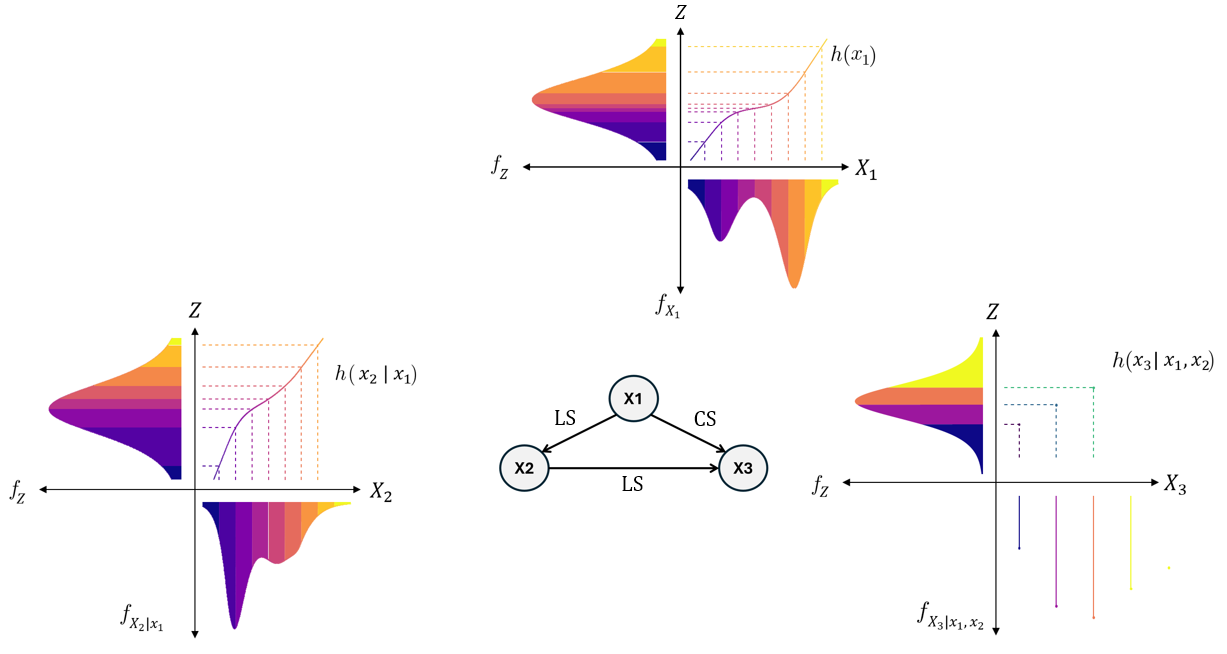
\includegraphics[width=0.9\textwidth]{img/tram_dag.png}
\caption{Example of a TRAM-DAG with three variables $X_1$, $X_2$ and $X_3$. The transformation functions are represented by the modular neural networks. The arrows indicate the causal dependencies between the variables.}
\label{fig:tram_dag}
\end{figure}

This DAG with the assumed dependencies can be described by an adjacency matrix \ref{eq:MA}, where the rows indicate the source and the columns the target of the effect: 


\begin{equation}
\mathbf{MA} =
\begin{bmatrix}
  0 & \text{LS} & \text{LS} \\
  0 & 0  & \text{CS} \\
  0 & 0  & 0
\end{bmatrix}
\label{eq:MA}
\end{equation}

To apply the framework of TRAM-DAGs on this example, we assume to have observational data that follows the structure of the adjacency matrix \ref{eq:MA}. In practice, the DAG is either defined by expert knowledge or by some sort of structure finding algorithm (XXX cite methods). Then we want to estimate the conditional distribution function of each variable by a deep TRAM so that we can sample from the distributions and make causal queries. The conditional distribution functions are given by


\[
\begin{aligned}
X_1 &\sim F_Z(h_I(x_1)) \\
X_2 &\sim F_Z(h_I(x_2) + \mathrm{LS}_{x_1}) \\
X_3 &\sim F_Z(h_I(x_3) + \mathrm{LS}_{x_1} + \mathrm{CS}_{x_2})
\end{aligned}
\]


\textbf{Construct Modular Neural network}

As discussed in the section \ref{sec:deep_trams}, the transformation functions are constructed by a modular neural network. The inputs are the variables in the system as well as the adjacency matrix \ref{eq:MA} which controls the information flow and assures that only valid connections according to the causal dependence are made. Discrete variables with few categories are dummy encoded, and continuous variables are scaled before feeding them in the neural network. The encoding and the effect of scaling on the interpretation of parameters is discussed in the appendix (ref XXX). The outputs are the three components for the transformation function (SI, LS, CS) for each variable. These components are assembled to the transformation functions. For the complex shift and complex intercept, the structure of the neural network (depth and width) has to be defined. 
Finally the loss is defined as the negative log likelihood, which the model aims to optimize to estimate the optimal parameterization. 


Describe interpretation quickly and refer to formal proof in the Appendix.
%  for interpretation see pearl book 2009 p. 366. the key is to say leaving all other variables "untouched" and not "constant". he also talks about the connection to the do-operator.

Finally, neural network works best if inputs are scaled. Proof that we can do that, it just changes the interpretation. For structure finding algorithms, this might be problematic, because increasing variance along the causal order would be destroyed. (why, how, interpretation change etc. check meeting notes 22.04.2025)

Fitting Betas Interpretable

The two parameters for our linear shift terms are plotted here. We can see that they converge quickly to the same values as we used in the DGP. We can interpret these parameters as log-odds ratios if changing the value of the parent by one unit.

Intercepts

Show the Discrete case with just cutpints (only K-1 parameters of outputs are used)
Show the continuous case where the outputs are transformed to monotonically increasing betas for the bernstein polynomial. Also describe Bernstein polynomial construction in detail with scaling and linear extrapolation.

Here I plotted the intercepts of the 3 transformation functions. They also resemble the DGP very nicely.


Linear and complex shifts

Here in the first two plots we can see the linear shifts. And in the right plot we have the complex shift of X2 on X3. The estimated shifts match quite well with the DGP.

Complex shift (Interaction example) to show what is also possible

Here I just want to make a short input from another example. So there the true model was that of a logistic regression with the binary outcome Y and 3 predictors. The binary treatment T and the two continuous predictors X1 and X2. There was also an interaction effect assumed between treatment and X1. So this basically means that the effect of X1 on the outcome is different for the two treatment groups.

And here we can show that our TRAM-DAG specified by a complex shift of T and X1 can also capture this interaction effect quite well.






\subsection{Sampling from TRAM-DAGs}

\textbf{Observational sampling} Once the TRAM-DAG is fitted on data, it can be used to sample from the observational or interventional distribution or to make counterfactual queries. 
The structural equations $X_i = f(Z_i, \text{pa}(X_i))$ are represented by the inverse of the conditional transformation functions $h^{-1}(Z_i \mid \text{pa}(X_i))$ because $Z_i = h(X_i \mid \text{pa}(X_i))$. The sampling process from the observational distribution for one iteration (one observation of all variables in the DAG) is described in the pseudocode \ref{alg:sampling} and illustrated in Figure~\ref{fig:sampling}. The process is repeated for the desired number of samples. 

\begin{algorithm}
\caption{Generate a samples from the TRAM-DAG}
\label{alg:sampling}
\begin{algorithmic}[1]
\State \textbf{Given:} A fitted TRAM-DAG with structural equations $X_i = f(Z_i, \text{pa}(X_i))$, where $Z_i = h(X_i \mid \text{pa}(X_i))$
\For{each node $X_i$ in topological order}
  \State Sample latent value $z_i \sim F_{Z_i}$ \Comment{e.g., \texttt{rlogis()} in R}
  \If{$X_i$ is continuous}
    \State Compute $x_i = h^{-1}(z_i \mid \text{pa}(x_i))$ by solving $h(x_i \mid \text{pa}(x_i)) - z_i = 0$
    \EndIf
  \If{$X_i$ is discrete}
    \State Determine $x_i$ such that $x_i = \min \left\{ x : z_i \le h(x \mid \text{pa}(x_i)) \right\}$
  \EndIf
\EndFor
\end{algorithmic}
\end{algorithm}


\begin{figure}[H]
\centering
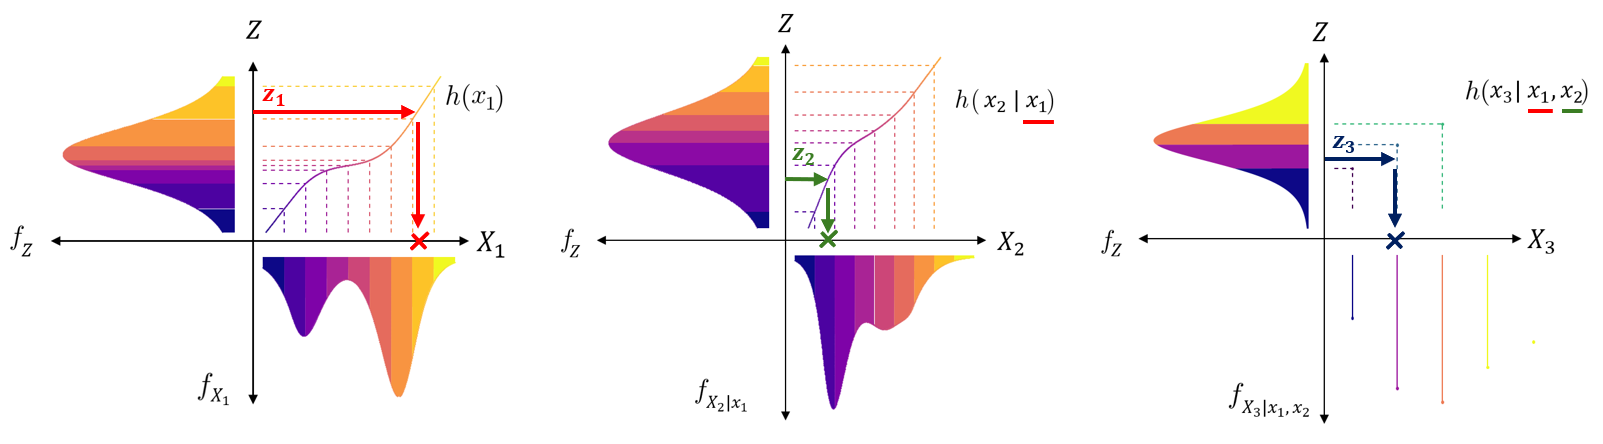
\includegraphics[width=0.9\textwidth]{img/sampling.png}
\caption{One sampling iteration for the three variables from the estimated transformation functions $h(x_i \mid \text{pa}(x_i))$. The latent values $z_i$ are sampled from the standard logistic distribution. The values $x_i$ are determined by applying the inverse of the transformation function for continuous variables or by finding the corresponding category for the ordinal variable.}
\label{fig:sampling}
\end{figure}


\textbf{Interventional sampling} To sample from the interventional distribution, we can apply the do-operator as described by \citet{pearl1995} (Pearl named it set instead of do). The do-operator fixes a variable at a certain value and sample from the distribution of the other variables while keeping the fixed variable constant. For example, if one wants to intervene on $X_2$ and set it to a specific value $\alpha$, $\textcolor{red}{\text{do}(x_2 = \alpha})$
and then sample from the interventional-distribution
\[
x_3 = \min \left\{ x : z_3 \le h(x \mid x_1, \textcolor{red}{x_2 = \alpha}) \right\}
\]

with the same process as for the observational sampling, with the only difference that the intervened variable $X_2$ stays constant.





\textbf{Counterfactual queries} In a counterfactual query one wants to know what the value of variable $X_i$ would have been if another variable $X_j$ had a different value than what was acutally observed. \citet{pearl_book2009} describes the three-step process to answer counterfacutal queries as follows: Given a causal model $M$ and observed evidence $e$ (which are the actually observed values of the variables $X_i$ of one sample) one wants to compute the probability of $Y=y$ under the hypothetical condition $X=x$.

Step 1 aims to explain the past (Z) by knowledge of the evidence e; 
Step 2 amends the past to the hypothetical condition $X=x$ 
Step 3 predicts the future (Y) based on our new understanding of the past and our newly established condition, $X =x$

Pearl named these three steps, (1) abduction,  (2) action and (3) prediction. The procedure is described in the pseudocode \ref{alg:counterfactual} and illustrated in Figure.

\begin{algorithm}
\caption{Answer a Single Counterfactual Query}
\label{alg:single_cf}
\begin{algorithmic}[1]
\State \textbf{Given:} A structural model $X_k = f(Z_k, \text{pa}(X_k))$, with inverse noise map $Z_k = h(X_k \mid \text{pa}(X_k))$
\State \textbf{Input:} Observed sample $x$, intervention $X_i := \alpha$, target variable $X_j$
\vspace{0.3em}
\State \textbf{Step 1: Abduction} Infer latent variable $Z_j = h(x_j \mid \text{pa}(x_j))$ using the observed values
\vspace{0.3em}
\State \textbf{Step 2: Action} Replace the value of $X_i$ with $\alpha$ in the set of parent variables
\vspace{0.3em}
\State \textbf{Step 3: Prediction} Compute the counterfactual value $x_j^{cf} = h_j^{-1}(Z_j \mid \text{pa}(x_j)^{cf})$
\vspace{0.3em}
\end{algorithmic}
\end{algorithm}



While the probability of Y under the hypothetical condition $X=x$ can be determined in any case, the actual counterfactual value of Y is only defined for a continuous outcome but not for discrete outcomes.

% see pearl book causality: 1.4.4 Counterfactuals in Functional Models (page 36)

(What pearl writes:  Likewise, in contrast with the potential-outcome framework, counterfactuals in the structural account are not treated as undefined primitives but rather as quantities to be derived from the more fundamental concepts of causal mechanisms and their structure. )


\textbf{ITE how it is applied in our model?}

% \citet{hoogland2021} gave guidance on how ITE estimation should be performed. A crucial aspect is the consideration is the model complexity and the susceptibility to overfitting. Also the decision whether a HGL or HTE model should be applied. (Especially include stuff from Practical Considerations part , quite good)
% RCTs only measure the average treatment effect. There will be patients who respond better or worse to the treatment because patient specific characteristcs. In personalized medicine however, the aim is to find the optimal treatment for a specific individual. Such a measure that can help in decision making is the ITE.

Rubins potential outcomes framework.


simulation studies
 "The setup was such that development and test sets were generated from the same data generating mechanism. In practice, there may be differences between these two settings that are not captured by the models, and the uncertainty that accompanies these unknowns may overshadow relatively small gains realized by more complex models."
 % https://pmc.ncbi.nlm.nih.gov/articles/PMC9291969/#sim9154-bib-0065
 
 "This could include the analysis of individual patient data from multiple randomized trials, or even the use of nonrandomized studies for the estimation of outcome risk under a control condition." this motivates the need for observational modeling.


Maybe it is the methods section. Here however, we give a couple hints.
Note that you can wisely use \rr{preamble}-chunks. Minimal, is likely:



Problems with ITE: (in an RCT setting)
- to estimate the ITE we must assume un-confoundedness. Does this also apply to itneractions (effect modifiers)? Check how this is handled in the literature.
- when there are treatment covariate interactions and these covariates are in the DGP but dropped from the dataset (so unobserved), then the ITE Estimation failed in the simulations. At least when there is only 1 strongly interacting variable and we drop this one. An example could be the psychological condition of a patient which might also affect how the treatment works, this is not a confounder but an effect modifier, and i would assume that this variable is rarely recorede or measured.

- Maybe a good conclusion: because this problematic with missing effect modifiers in RCT data can be a motivation to work with observational data where the dag is very detailed specified with all confounders and interactions, then a tram-dag can be applied. However, there we also have the problem, that important variables are probably also not known/measured...

- question still to answer: the estimated ITE on the train vs test set is equally bad (in terms of scatterplot and RMSE), so why does the ITE-cATE plot and the ITE Outcome plot looks like it discriminates good in the train set but not in the test set? Could the answer be, that the model is overfitting, hence tries to really model the observed outcomes and not the true probabilities, hence when an inportant variable is missing, it could still reasonably well predict the outcome (probability) but these are not the causal relationships anymore, so therefore the ITE estimation is bad on the train and the test set. But the ITE-cATE plot still looks good in the train set, because at least the observed outcomes could be predicted very well.??? still not sure if this is the case and how to proof.

- another point is the effect of the correlation of the variables. If the X's are strongly correlated, and one X with interaction effect is dropped, can the info then still be retreived from the other variables? maybe the effect is then attributed to another correlated variable. --> check with simulations and or theroretical proof.


- maybe also make propensity score estimation on IST stroke trial to check if possibly confounded.

- also talk about propensity score Rubin(2007) to basically estimate an RCT...and overcome the problem of confounding. but this might work for ATE but not really for ITE, direct modelling of the outcome is necessary % https://pmc.ncbi.nlm.nih.gov/articles/PMC5920646/


\textbf{Models for ITE Estimation}

T-learner vs s-learner, metalearner,

The ITE for a binary endpoint is estimated as the difference of two probabilities (the risk under treatment minus the risk under control). It is essential that the model used to estimate these probabilities is well calibrated and generalizes to new (unseen) data. When using models that are estimated with conventional methods such as ordinary least squares or standard maximum likelihood, they tend to overfit on the training data and make too extreme predictions on the test data. This problem increases with reduced sample size, low event rate or large number of predictor variables. To prevent such overfitting, penalization (shrinkage) methods are proposed as they shrink the estimated coefficients towards zero to reduce the variance in predictions on new data \citep{riley2021}. 


Logistic regression, penalized logistic regression (shrinkage, lasso
Shrinkage methods should provide better predictive perfomance on average (cite articles). \citet{calster2020} analyzed different regression shrinkage methods with a binary outcome in a simulation study. They concluded, although the calibration slope improved on average, shrinkage often worked poorly on individual datasets. With small sample size and low number of events per variable the performance of most of these methods were highly variable and should be used with caution in such settings. \citet{riley2021} obtained to similar results in their simulation study. Problems occur, because tuning parameters are often estimated with large uncertainty on the training data and fail to generalize. In both studies the autors pointed out that these penalization methods are more unreliable when needed most, that is when the risk of overfitting may be large.

In this thesis , I will apply Lasso regression on the IST stroke trial and simulation studies, where the sample size is relatively large.

\section{Experiments}

\subsection{TRAM-DAG simulation}

Show easy simulation with 3 variables and in the results the plots of the loss function, the coefficient learning, intercepts, shifts, and the sampling results. The sampling results should show that the sampled data matches the DGP very well. Also show the estimated parameters of the linear shifts and the intercepts. The complex shift can be shown by plotting the transformation function of X3 with respect to X2. also some queries for observational, interventional and counterfactual.

\subsection{TRAM-DAG real data}

maybe the Weather data case, or another if we find a practical observational data example.

\subsection{ITE simulations}

Show types of models that will be applied and dgp and when problems occure.

\subsection{ITE real data}

% describe the data of stroke trial https://pubmed.ncbi.nlm.nih.gov/9174558/
Results on IST trial wiht the interpretation in the discussion part.

show results of different models including tram dag.



\section{Software}

All code was done in R wiht packages xx ussed for yy.

\bigskip

\hrule
\begin{knitrout}
\definecolor{shadecolor}{rgb}{0.969, 0.969, 0.969}\color{fgcolor}\begin{kframe}
\begin{verbatim}
library(knitr)
opts_chunk$set(
    fig.path='figure/ch02_fig',
    self.contained=FALSE,
    cache=TRUE
)
\end{verbatim}
\end{kframe}
\end{knitrout}
\hrule

\bigskip

Defining figure options is very helpful:


\bigskip


\hrule
\begin{knitrout}
\definecolor{shadecolor}{rgb}{0.969, 0.969, 0.969}\color{fgcolor}\begin{kframe}
\begin{verbatim}
library(knitr)
opts_chunk$set(fig.path='figure/ch02_fig',
               echo=TRUE, message=FALSE,
               fig.width=8, fig.height=2.5,
               out.width='\\textwidth-3cm',
               message=FALSE, fig.align='center',
               background="gray98", tidy=FALSE, #tidy.opts=list(width.cutoff=60),
               cache=TRUE
)
options(width=74)
\end{verbatim}
\end{kframe}
\end{knitrout}
\hrule

\bigskip

This options are best placed in the main document at the beginning. Otherwise a \verb+cache=FALSE+ as knitr option is necessary to overrule a possible  \verb+cache=TRUE+ flag.

\bigskip

Notice how in Figure~\ref{f02:1} everything is properly scaled.

\begin{figure}
\begin{knitrout}
\definecolor{shadecolor}{rgb}{0.98, 0.98, 0.98}\color{fgcolor}

{\centering 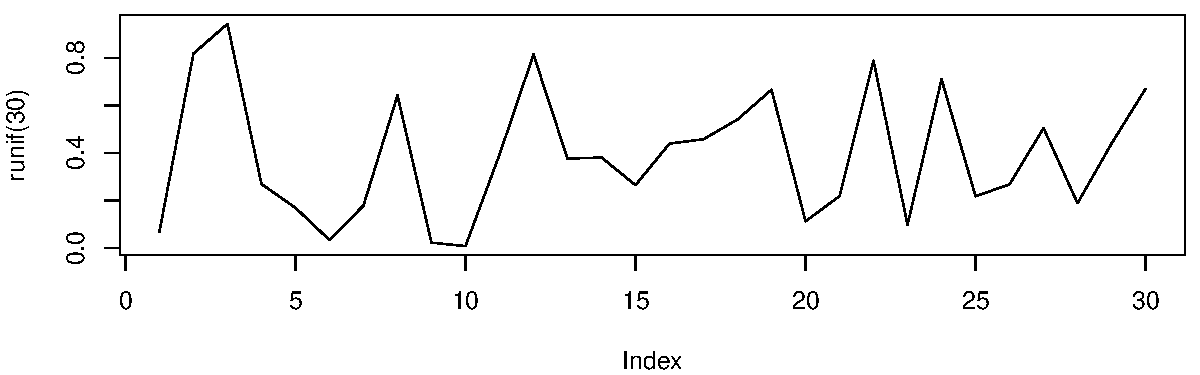
\includegraphics[width=\textwidth-3cm]{figure/ch02_figunnamed-chunk-3-1} 

}


\end{knitrout}
  \caption{Test figure to illustrate figure options used by knitr.}
  \label{f02:1}
\end{figure}


\section{Citations}

Recall the difference between \verb+\citet{}+ (e.g., \citet{Chu:Geor:99}), \verb+\citep{}+ (e.g., \citep{Chu:Geor:99}) and \verb+\citealp{}+ (e.g., \citealp{Chu:Geor:99}).
For simplicity, we include here all references in the file \verb+biblio.bib+ with the command \verb+\nocite{*}+.\nocite{*}



%%%%%%%%%%%%%%%%%%%%%%%%%%%%%%%%%%%%%%%%%%%%%%%%%%%%%%%%%%%%%%%%%%%%%%
%%%%%%%%%%%%%%%%%%%%%%%%%%%%%%%%%%%%%%%%%%%%%%%%%%%%%%%%%%%%%%%%%%%%%%


% 

% LaTeX file for Chapter Exp1



\chapter{Experiment 1: TRAM-DAG (simulation)}




\section{Motivation}

This experiment demonstrates the application of TRAM-DAGs on a synthetic dataset, using the illustrative DAG previously shown in Figure~\ref{fig:tram_dag}. The objective is to show how TRAM-DAGs can learn causal relationships from observational data, assuming a known DAG. After fitting the model to the joint distribution generated by the underlying causal structure, it is used to sample from observational, interventional, and counterfactual distributions.

The controlled simulation setting allows us to interpret the learned model components in detail and evaluate the model’s ability to recover both linear and nonlinear causal relationships.



% \section{Setup} \label{sec:methods_experiment1}

% To evaluate the TRAM-DAG model, we visualize training performance through the loss curve, interpret the learned transformation components (e.g., intercepts, linear and complex shifts), and assess the model's ability to recover the true data-generating process (DGP). We then sample from the learned model to generate observational and interventional distributions and perform counterfactual queries.


\section{Setup} \label{sec:methods_experiment1}

We visualized the model fitting in terms of the training loss and subsequently showed and interpreted the learned components of the transformation functions, such as intercepts, linear and complex shifts. Finally, we drew samples from the estimated distributions to obtain observational and interventional distributions. We also conducted counterfactual queries on the learned model.

\medskip

\textbf{Data-generating process: } We simulated a dataset with three variables, $X_1$, $X_2$, and $X_3$, following the structure of the DAG and its associated meta-adjacency matrix shown in Figure~\ref{fig:dag_and_matrix}. The matrix describes the functional dependencies between variables, where LS indicates a linear shift and CS a complex shift. Rows represent the source of the effect, and columns the target.


\begin{figure}[H]
\centering
\begin{tikzpicture}[baseline={(current bounding box.center)}]
  \node (img) at (0, 0) {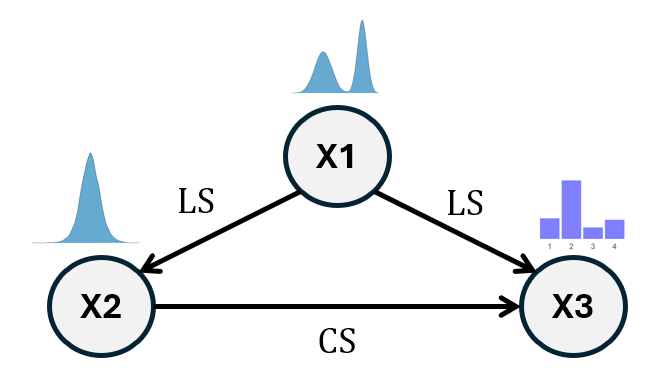
\includegraphics[width=0.28\textwidth]{img/exp1_DAG_MA.png}};
  \node (matrix) at (5, 0) {
    $\mathbf{MA} =
    \begin{bmatrix}
      0 & \text{LS} & \text{LS} \\
      0 & 0  & \text{CS} \\
      0 & 0  & 0
    \end{bmatrix}$
  };
  \draw[->, thick] (img.east) -- (matrix.west);
\end{tikzpicture}
\caption{Causal graph (left) and meta-adjacency matrix (right) for Experiment 1. The transformation function of $X_2$ depends on $X_1$ via a linear shift (LS). The transformation function of $X_3$ depends on $X_1$ via a linear shift (LS) and on $X_2$ via a complex shift (CS).}
\label{fig:dag_and_matrix}
\end{figure}

The variable $X_1$ is continuous and bimodally distributed, and acts as a source node in the DAG, i.e., it is not influenced by any other variable:

\[
X_1 = 
\begin{cases}
\mathcal{N}(0.25,\, 0.1^2) & \text{with probability } 0.5, \\
\mathcal{N}(0.73,\, 0.05^2) & \text{with probability } 0.5
\end{cases}
\]


    
The second variable, $X_2$, is continuous and linearly dependent on $X_1$ on the log-odds scale, with a true coefficient of $\beta_{12} = 2$. Its transformation function is 
\[
h(X_2 \mid X_1) = h_I(X_2) + \beta_{12} X_1,
\]
where the baseline transformation (i.e., intercept) of $X_2$ is $h_I(X_2) = 5 X_2$.

The third variable, $X_3$, is ordinal and depends on both $X_1$ (LS) and $X_2$ (CS). We define the complex shift induced by $X_2$ as $f(X_2) = 0.5 \cdot \exp(X_2)$, and specify the linear shift parameter for $X_1$ as $\beta_{13} = 0.2$. The transformation function for category $k$ of the ordinal variable $X_3$ with 4 levels ($K$) is thus defined by 
\[
h(X_{3,k} \mid X_1, X_2) = \vartheta_k + \beta_{13} X_1 + f(X_2),
\]
with cut-points $\vartheta_k \in \{-2,\, 0.42,\, 1.02\}$ defining the thresholds of the ordinal variable. We generated samples for $X_2$ and $X_3$ as described in Section~\ref{methods:sampling}, by first sampling a latent value from the standard logistic distribution and then determining the corresponding observation using the transformation function.

This simulation allows us to assess whether the TRAM-DAG model can correctly recover the functional forms of the conditional dependencies and the associated parameters (linear and complex).

\medskip

\textbf{Model:} Given the meta-adjacency matrix and the simulated observations, we construct a modular neural network based on the TRAM-DAG framework. The complex shift from $X_2$ to $X_3$ is modeled using a neural network with 4 hidden layers and 2 nodes per layer, as illustrated in Figure~\ref{fig:exp1_CS}. A total of 20,000 samples are generated according to the defined DGP to fit the model. The model is trained for 400 epochs using the Adam optimizer \citep{kingma2015} with a learning rate of 0.005.


% include the figure for CS

\begin{figure}[H]
\centering
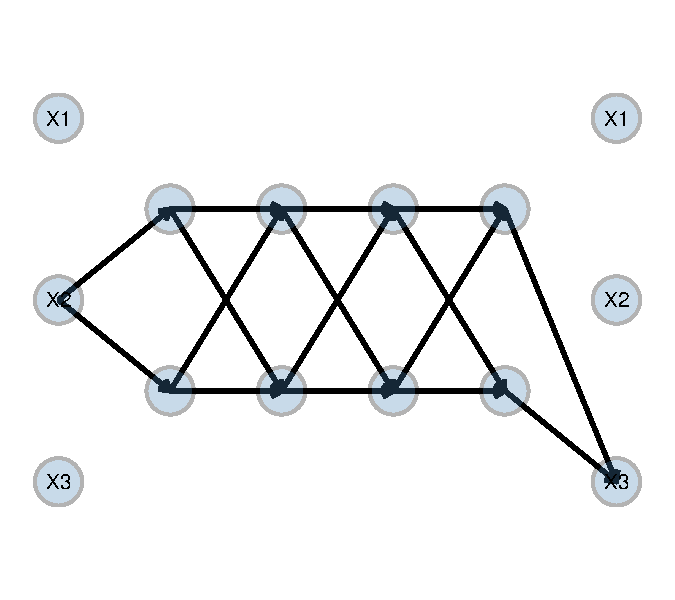
\includegraphics[width=0.5\linewidth]{img/exp1_CS.pdf}
\caption{Neural network architecture for the complex shift on $X_3$ from $X_2$. The complex shift is modeled by a neural network with 4 hidden layers of shape (2, 2, 2, 2), using non-linear activation functions (sigmoid).}
\label{fig:exp1_CS}
\end{figure}




\textbf{Model evaluation: } We compare the estimated intercepts, learned coefficients, and the complex shift to the true values used in the DGP. We also compare the sampled observational and interventional distributions to the true distributions. For the counterfactual queries, we show the estimated counterfactual values for $X_2$ under an intervention on $X_1$ at a specific value, and compare these to the true counterfactual outcomes.




\section{Results}



We evaluate whether TRAM-DAGs can recover the structural equations and distributions used in the data-generating process described in Section~\ref{sec:methods_experiment1}. Below, we present the training process and inspect the estimated parameters, distributions, and counterfactual predictions.

Figure \ref{fig:exp1_loss_parameters} shows the loss and the estimated parameters for the linear shifts over epochs during training. The loss was minimized during training and the estimated parameters $\beta_{12}$ and $\beta_{13}$ converged to the true values used in the DGP. The linear shift parameters are the interpretable part of the model (log-odds ratios). From the fitted model, we generated samples from the observational distribution, as shown in Figure \ref{fig:exp1_observational_distribution}. The TRAM-DAG can recover the observational distribution as its samples align with the data that was used to fit the model. Then we drew samples from the interventional distribution, where $X_2 = 1$ is fixed, as shown in Figure \ref{fig:exp1_interventional_distribution}. Fixing $X_2$ leads to a distributional change in $X_3$, which was also captured by the model. The TRAM-DAG learns the linear shifts ($\beta_{12}$, $\beta_{13}$) and the complex shift $f(X_2)$, which are shown in Figure \ref{fig:exp1_shifts}. Figure~\ref{fig:exp1_intercepts} presents the intercepts learned for each of the nodes. For comparison, we added the estimated intercept functions from the Continuous Outcome Logistic Regression (Colr() function from the \texttt{tram} package \citep{hothorn2018}) for $X_1$ and $X_2$, and the true values used in the DGP for the ordinal variable $X_3$ (three cut-points for the four levels). Since the transformation functions for $X_1$ and $X_2$ contain no complex terms, they match the default form used in Colr(). Finally, Figure~\ref{fig:exp1_counterfactuals} shows the counterfactuals for $X_2$ estimated by the TRAM-DAG for varying values of $X_1$. The counterfactuals are the predicted values of $X_2$ had $X_1$ taken other values instead of the initially observed one. 

\begin{figure}[htbp]
\centering
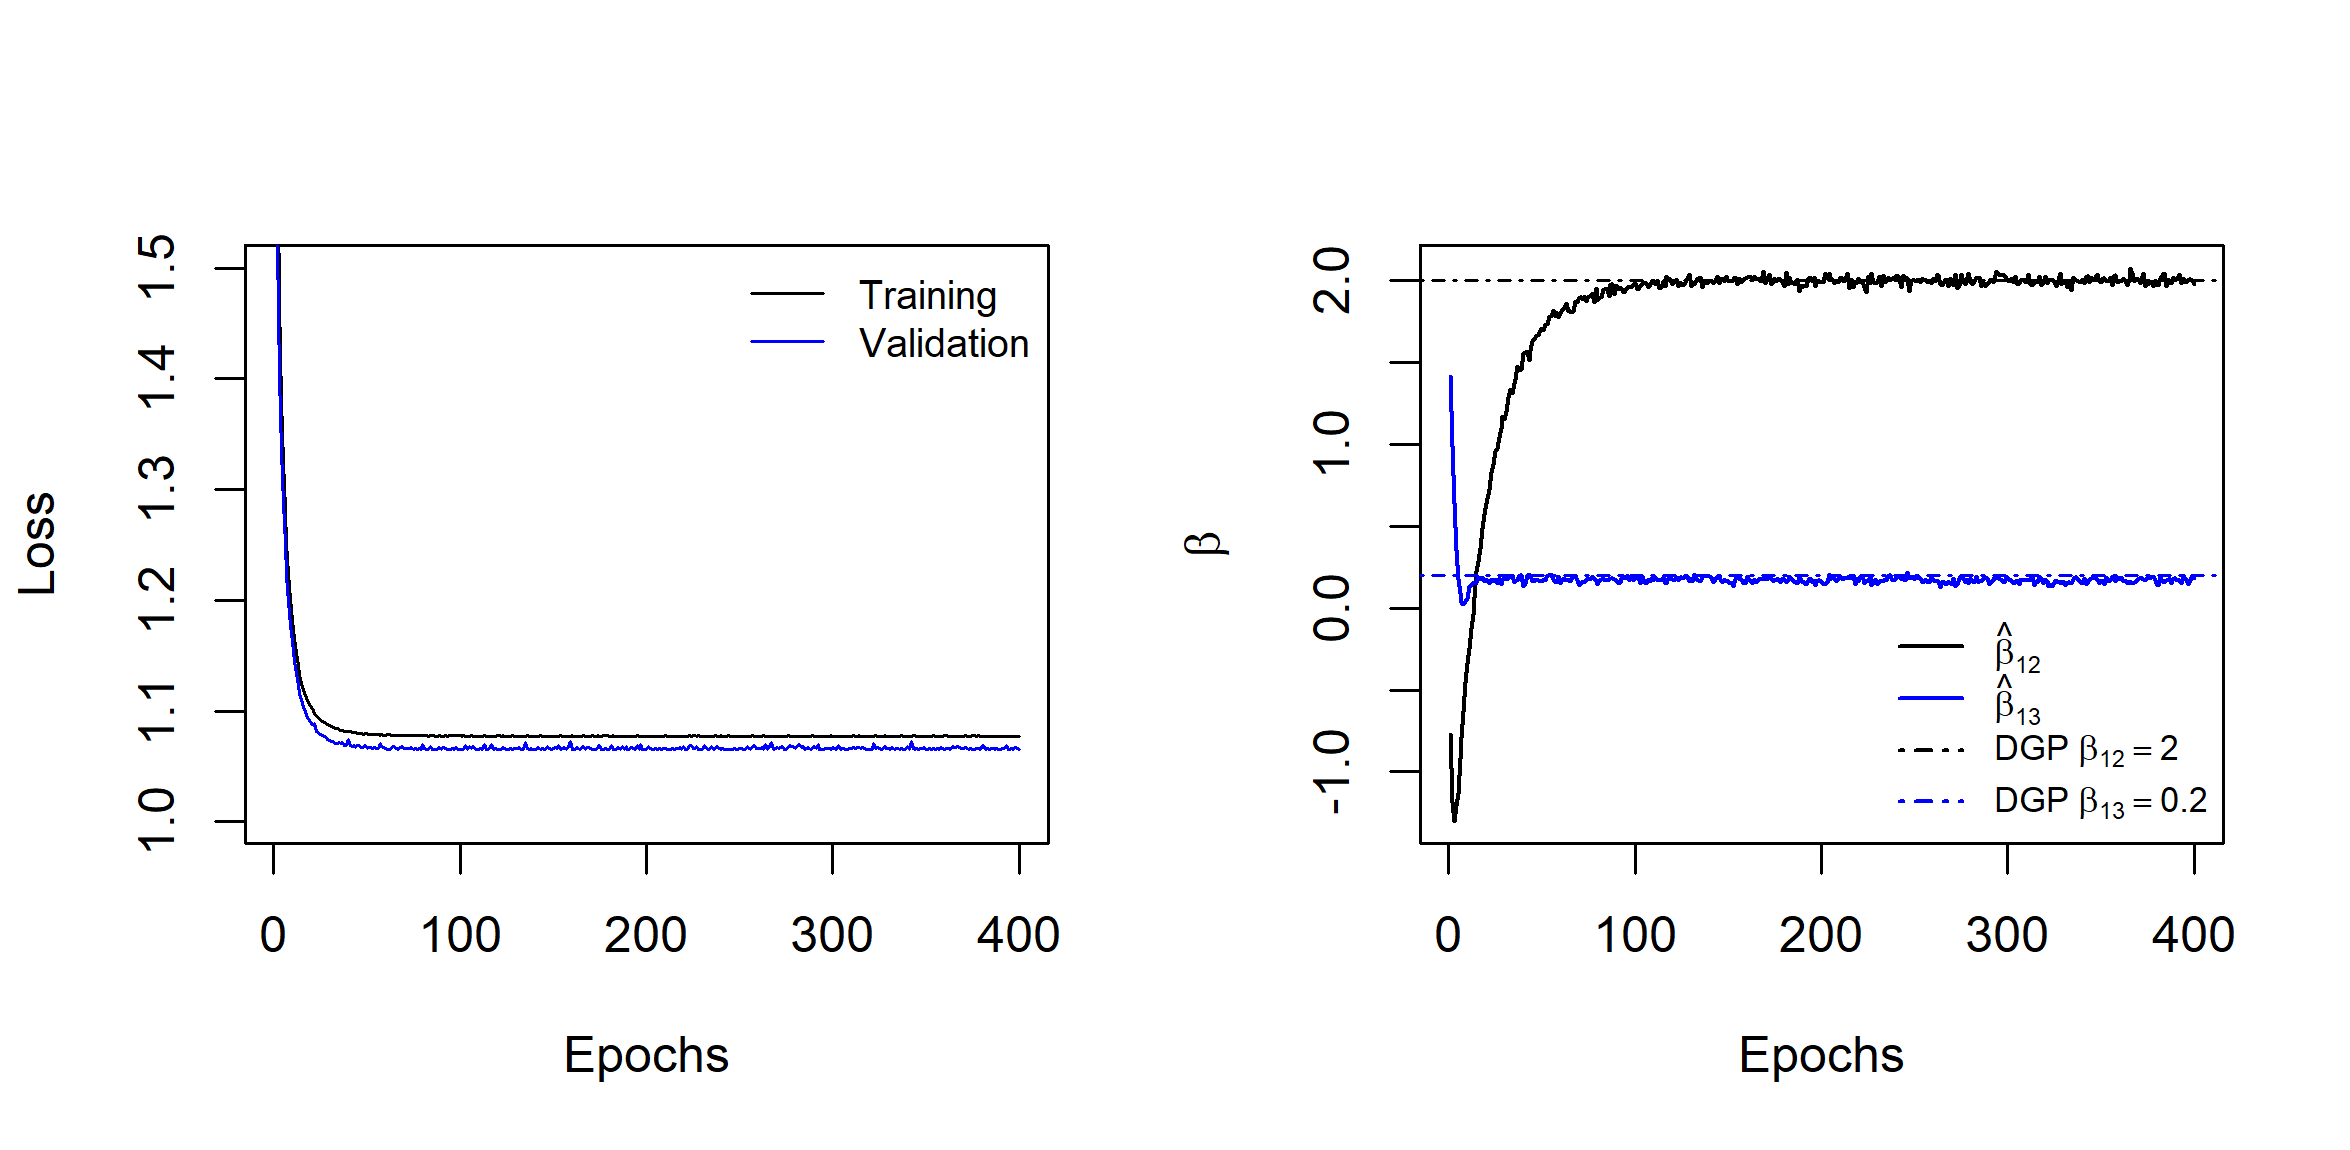
\includegraphics[width=0.9\textwidth]{img/exp1_loss_parameters.png}
\caption{TRAM-DAG model fitting over 400 epochs for Experiment 1. Left: loss functions on the training and validation sets; Right: estimated parameters (betas) for the linear shift components over epochs. The estimates converge to the true values used in the DGP.}
\label{fig:exp1_loss_parameters}
\end{figure}



\begin{figure}[htbp]
\centering
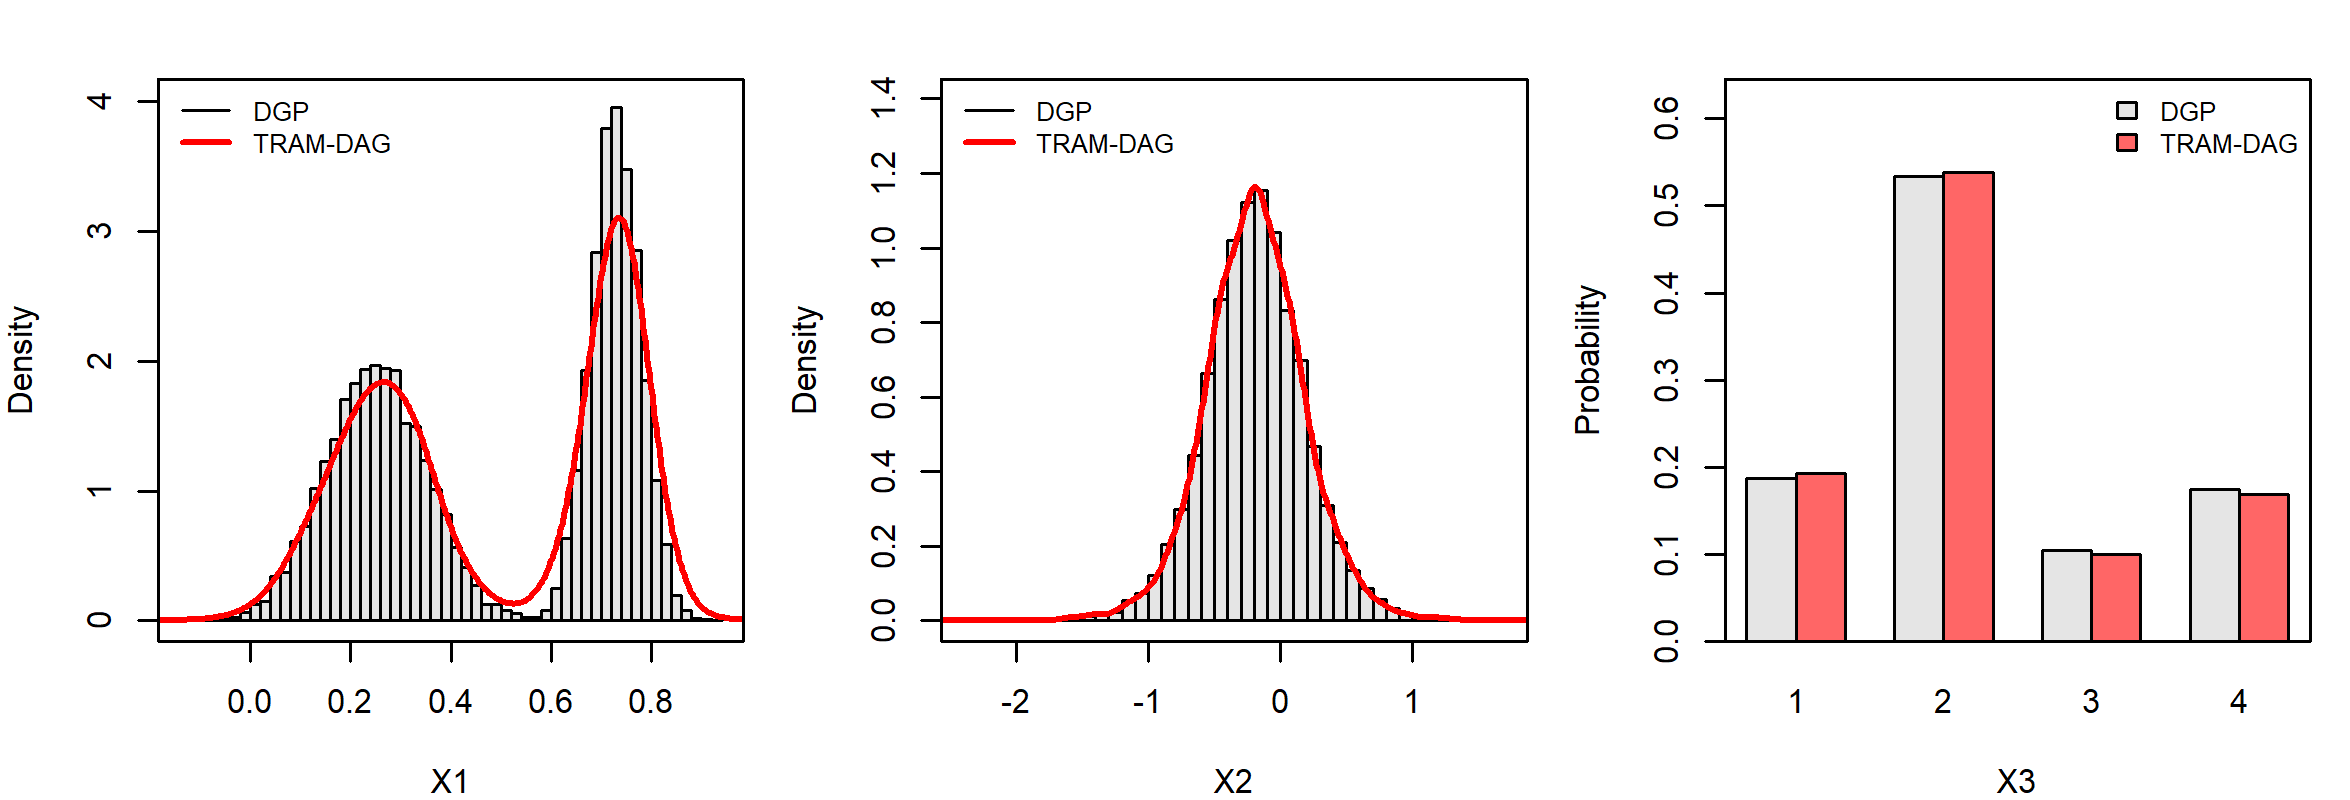
\includegraphics[width=0.9\textwidth]{img/exp1_observational_distribution.png}
\caption{Samples generated by the TRAM-DAG from the learned observational distribution, compared to the true observations from the DGP.}
\label{fig:exp1_observational_distribution}
\end{figure}




\begin{figure}[htbp]
\centering
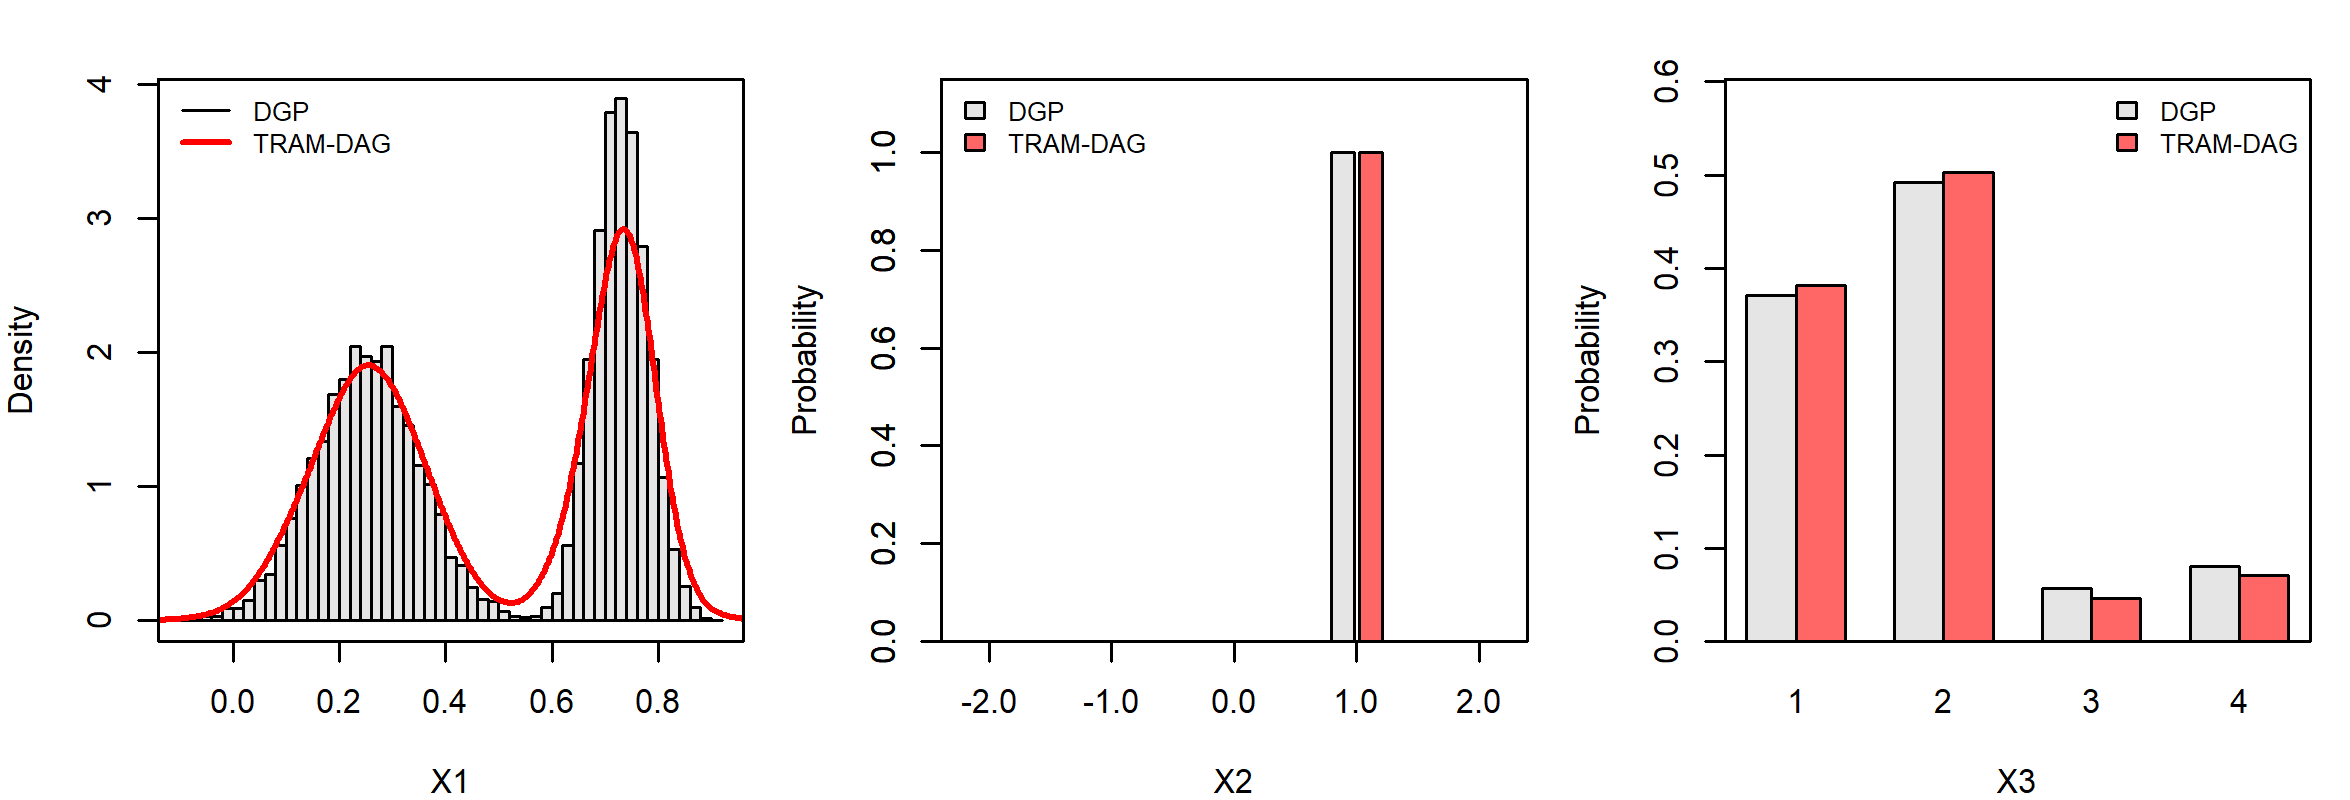
\includegraphics[width=0.9\textwidth]{img/exp1_interventional_distribution.png}
\caption{Samples generated by the TRAM-DAG compared to the true observations from the interventional distribution of the DGP, where $X_2 = 1$ is fixed. According to the DAG, this intervention induces a distributional change in $X_3$.}
\label{fig:exp1_interventional_distribution}
\end{figure}



\begin{figure}[htbp]
\centering
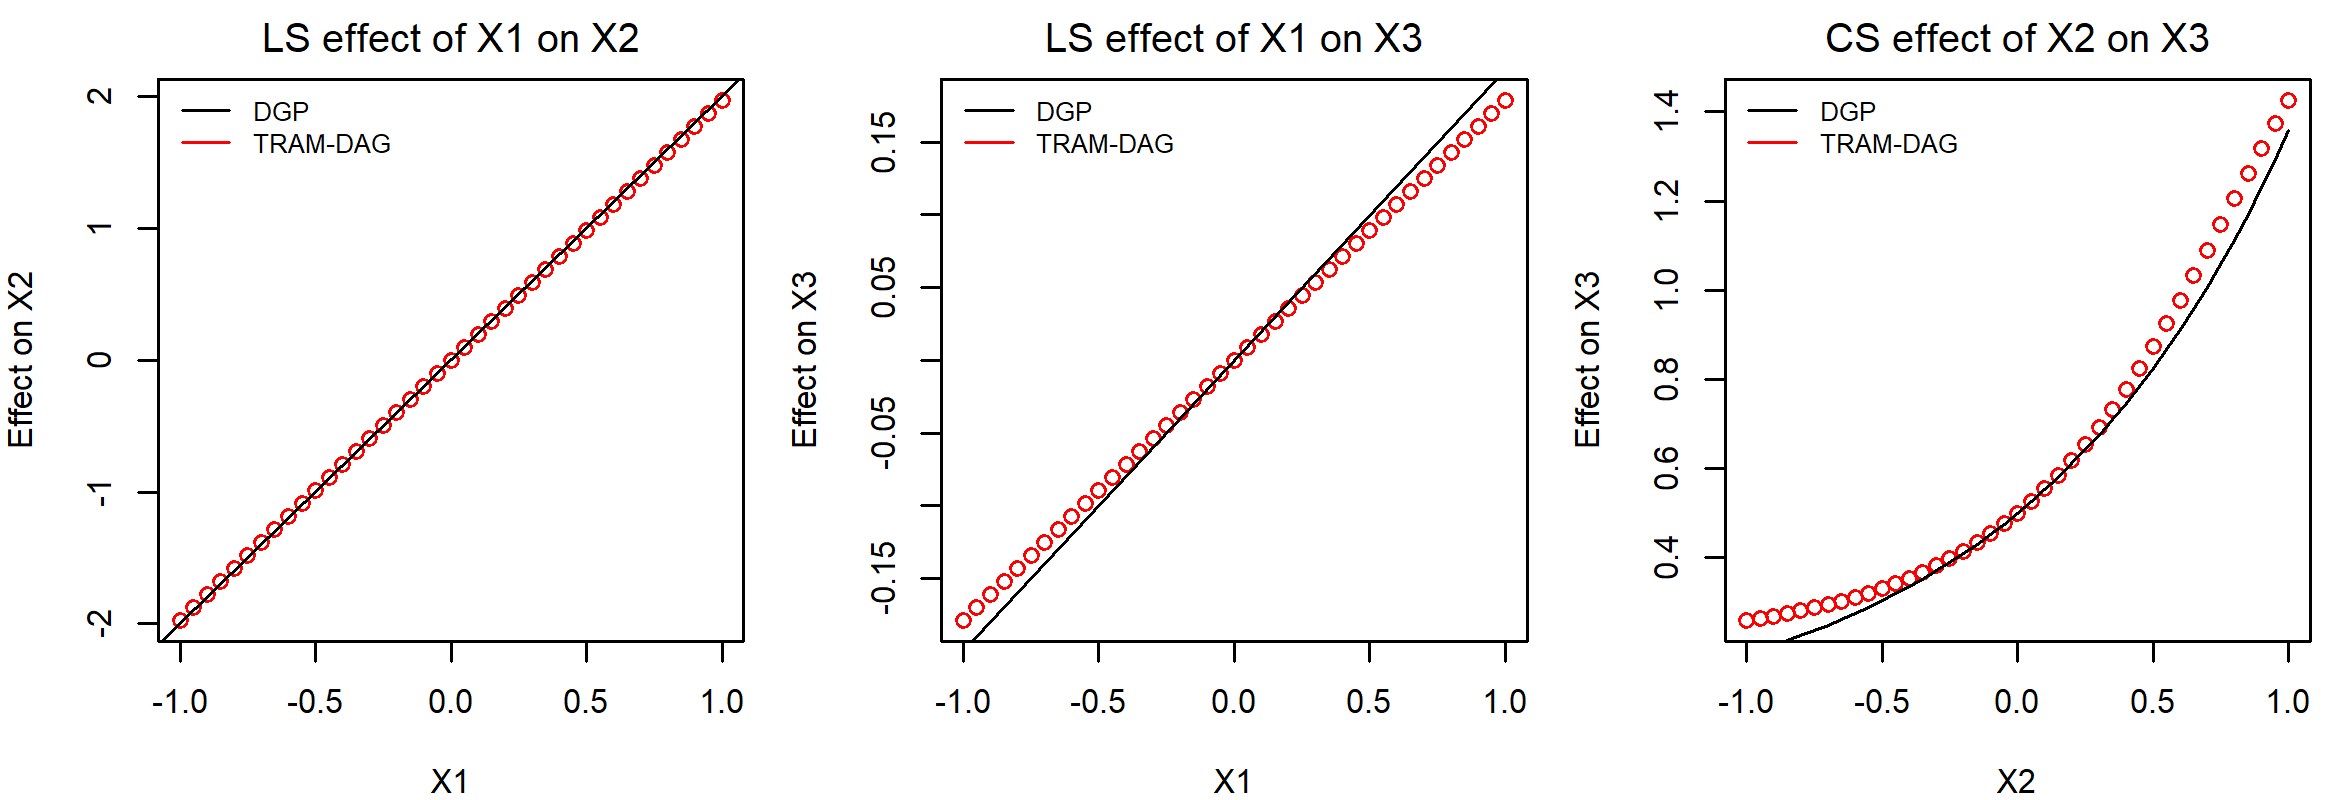
\includegraphics[width=0.9\textwidth]{img/exp1_LS_CS.png}
\caption{Linear and complex shifts learned by the TRAM-DAG. Left: LS($X_1$) on $X_2$; Middle: LS($X_1$) on $X_3$; Right: CS($X_2$) on $X_3$. For visualization, we subtracted $\delta_0 = \text{CS}(0) - f(0)$ from the estimated complex shift CS($X_2$) to align it with the true shift function $f(X_2)$ from the DGP.}
\label{fig:exp1_shifts}
\end{figure}



\begin{figure}[htbp]
\centering
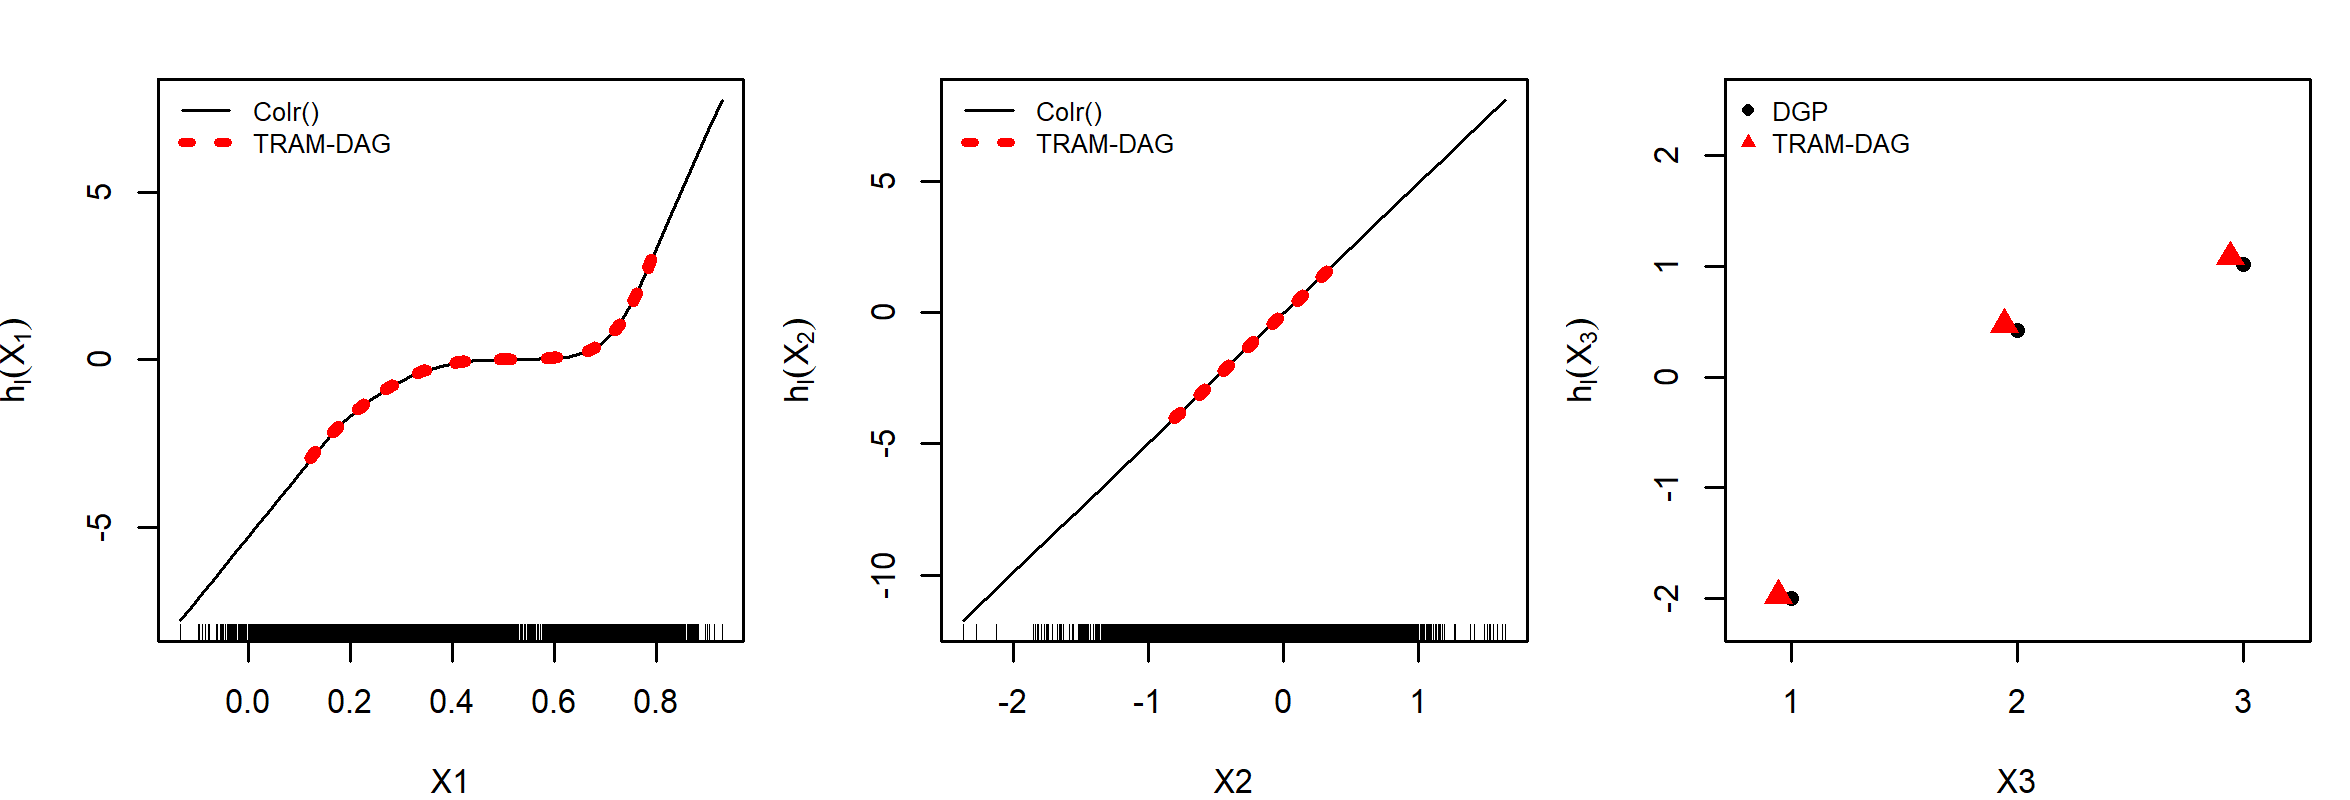
\includegraphics[width=0.9\textwidth]{img/exp1_baseline_trafo.png}
\caption{Intercepts learned for each of the nodes, along with the estimates from the \texttt{Colr()} function for the continuous variables and the true values from the DGP for the ordinal variable $X_3$. Left: Smooth baseline transformation function for continuous $X_1$; Middle: Smooth baseline transformation function for continuous $X_2$; Right: Cut-points as the baseline transformation function for ordinal $X_3$. For the last plot, we added $\delta_0 = \text{CS}(0) - f(0)$ to the estimated cut-offs to make them comparable to the true parameters from the DGP.}
\label{fig:exp1_intercepts}
\end{figure}




\begin{figure}[htbp]
\centering
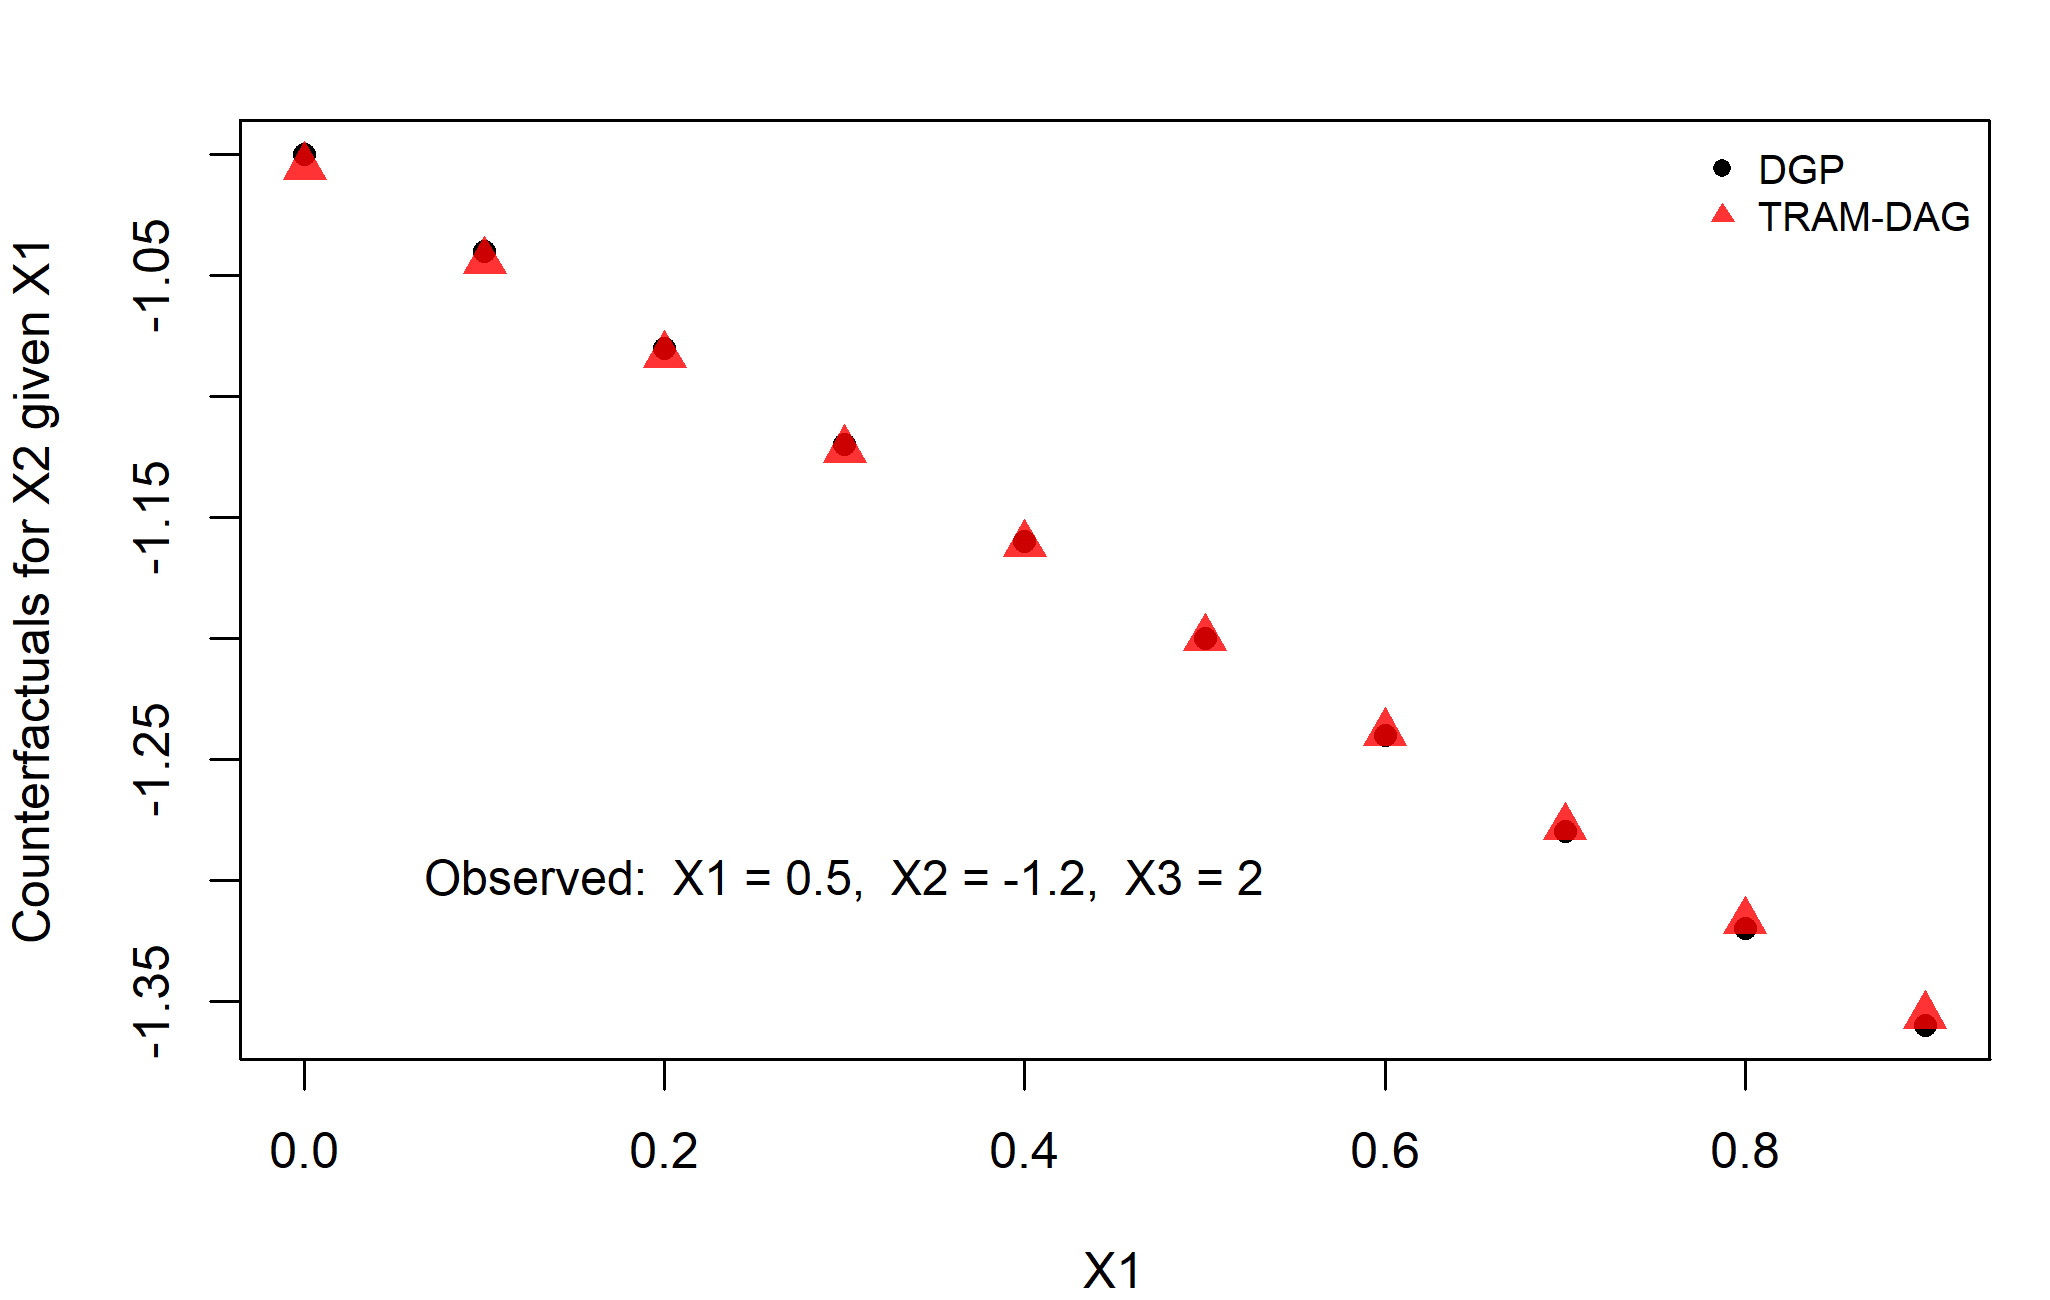
\includegraphics[width=0.9\textwidth]{img/exp1_counterfactuals.png}

\caption{Counterfactuals for $X_2$ estimated with the TRAM-DAG for varying values of $X_1$. We assumed the observed values $X_1 = 0.5$, $X_2 = -1.2$, and $X_3 = 2$, and determined the counterfactual values of $X_2$ had $X_1$ taken different values instead of the actually observed one. This illustrates how the model estimates alternative outcomes under hypothetical interventions on $X_1$.}
\label{fig:exp1_counterfactuals}
\end{figure}



% enforce that starts after all floats have been displayed
\FloatBarrier

\section{Discussion}

The results show that the TRAM-DAG framework can accurately recover the underlying causal relationships from data, including both linear and nonlinear (complex) relationships. This enabled the model to generate observational and interventional distributions that closely matched the true ones, and to produce valid counterfactual predictions.

This experiment provides a simple proof of concept for the flexibility and generative capability of TRAM-DAGs. By incorporating both interpretable (e.g., linear shifts) and flexible (e.g., complex shift) components, the model is able to capture a range of causal mechanisms -- provided that the true DAG is known and data is generated accordingly.


% \section{Discussion}
% 
% 
% The results demonstrate that the TRAM-DAG framework can learn the true parameters and both linear and complex shifts from the data, enabling it to act as a generative model for predicting interventions and counterfactuals. It successfully reproduced observational and interventional distributions and predicted correct counterfactual outcomes.
% 
% This experiment serves as a small proof of concept that TRAM-DAGs can be specified flexibly, with both interpretable and complex components, to capture causal relationships of varying complexity when the true DAG is known and the data is generated accordingly.





%%%%%%%%%%%%%%%%%%%%%%%%%%%%%%%%%%%%%%%%%%%%%%%%%%%%%%%%%%%%%%%%%%%%%%
%%%%%%%%%%%%%%%%%%%%%%%%%%%%%%%%%%%%%%%%%%%%%%%%%%%%%%%%%%%%%%%%%%%%%%

% 

% LaTeX file for Chapter Exp2






\chapter{Experiment 2: ITE on International Stroke Trial (IST)} \label{ch:exp2}





\section{Motivation}


% describe the data of stroke trial https://pubmed.ncbi.nlm.nih.gov/9174558/
% Results on IST trial with the interpretation in the discussion part.

%  here the authors made the IST database available and described the trial, we downloaded the CSV
% https://trialsjournal.biomedcentral.com/articles/10.1186/1745-6215-12-101 


% Results: The IST dataset includes data on 19 435 patients with acute stroke, with 99% complete follow-up. Over 26.4% patients were aged over 80 years at study entry. Background stroke care was limited and none of the patients received thrombolytic therapy.
% 
% 
\citet{chen2025} evaluated multiple causal ML methods on the International Stroke Trial (IST), to estimate the individualized treatment effects. They demonstrated that none of the applied ML methods generalized well, as performance on the test data differed significantly from the training data on the chosen evaluation metrics.
In this experiment, we replicate the analysis on the same data by applying three causal ML methods for ITE estimation, to investigate whether we obtain similar results as the authors.


\section{Setup} \label{sec:methods_experiment2}



\textbf{Data:} The International Stroke Trial was a large, randomized controlled trial conducted in the 1990s to assess the efficacy and safety of early antithrombotic treatment in patients with acute ischemic stroke \citep{IST1997}. Using a 2x2 factorial design, 19,435 patients across 36 countries were randomized within 48 hours of symptom onset to receive aspirin, subcutaneous heparin, both, or neither. Patients allocated to aspirin (300 mg daily for 14 days) had a 6-month death or dependency rate of 62.2\%, compared to 63.5\% in the control group not receiving aspirin, corresponding to a statistically significant absolute risk reduction after adjustment for baseline prognosis (1.4\%, p = 0.03). The authors stated that there was no interaction between aspirin and heparin in the main outcomes. In this thesis, we focus exclusively on the aspirin vs. no aspirin comparison and the outcome of death or dependency at 6 months after stroke.

The dataset used in this experiment was made publicly available by \citet{sandercock2011} and contains individual-level data, including baseline covariates assessed at randomization, treatment allocation, and 6-month outcomes, with a follow-up rate of 99\%.

We used the same data pre-processing steps as \citet{chen2025} to ensure comparability of results. 5.9\% of individuals had incomplete data and were removed from the dataset. We used 2/3 of the data for fitting the models and 1/3 as a hold out test set. The final dataset included 21 baseline variables recorded at randomization: aspirin allocation (treatment), age, delay between stroke and randomization (in hours), systolic blood pressure, sex, CT performed before randomization, visible infarct on CT, atrial fibrillation, aspirin use within 3 days prior to randomization, and presence or absence of neurological deficits (including face, arm/hand, leg/foot deficits, dysphasia, hemianopia, visuospatial disorder, brainstem or cerebellar signs, and other neurological deficits), as well as consciousness level, stroke subtype, and geographical region. The outcome variable was death or dependence at 6 months.


\medskip

\textbf{Models for ITE estimation: } The aim is to estimate the ITE based on baseline characteristics. As a benchmark, we apply a T-learner logistic regression (following \citet{chen2025}, using the \texttt{stats} package). As a more complex model, we apply a T-learner tuned random forest (using the \texttt{comets} package \citep{comets}), which tunes the number of variables considered for splitting at each node (\texttt{mtry}) and the maximum tree depth (\texttt{max.depth}) using out-of-bag error, with 500 trees. Additionally, we apply an S-learner TRAM-DAG. For the random forest and TRAM-DAG based methods, we additionally scale numerical and dummy encode categorical covariates prior to model training. The transformation function of the outcome is modelled by a complex intercept $h(Y \mid T, \mathbf{X}) = CI(T, \mathbf{X})$, with 4 hidden layers of shape (20, 10, 10, 2). This architecture allows for interaction between the treatment and covariates. Furthermore, batch normalization, ReLU activation, and dropout (0.1) are applied to prevent overfitting and stabilize learning. A validation set comprising 20\% of the training data is used to select the model with the lowest out-of-sample negative log-likelihood, while the test set remains untouched for final evaluation. 

Since the IST is a randomized controlled trial, the full potential of TRAM-DAGs -- designed primarily for use in observational settings -- is not required here, as only the outcome needs to be modeled as a function of baseline patient characteristics. However, applying TRAM-DAGs in this context still allows us to assess its predictive performance and ability to flexibly model interactions between variables.



\medskip

\textbf{Model evaluation: } For validation, since the ground truth is not known, we first rely on calibration plots to assess the general prediction power for the probabilities. Second, we predict the potential outcomes with the trained models to estimate the ITE on the training and test set in terms of the risk difference $\text{ITE}_i = \text{P}(Y_i=1|T=1, \mathbf{X}_i) - \text{P}(Y_i=1|T=0, \mathbf{X}_i)$. For visual validation, we show the densities of the estimated ITEs on both datasets, and the ITE-ATE plots to assess whether the estimated ITEs align with the observed outcomes.










% possible example of unobserved interaction:
% An example could be the psychological condition of a patient which might also affect how the treatment works, this is not a confounder but an effect modifier, and i would assume that this variable is rarely recorede or measured.




\section{Results} \label{sec:results_experiment2}


In this section, we present the results of the ITE estimation on the International Stroke Trial (IST) dataset. The observed average treatment effect (ATE), defined as $\text{P}(Y=1|T=1) - \text{P}(Y=1|T=0)$, was -2.4\% absolute risk reduction on the training set, with a 95\% confidence interval from -4.1\% to -0.6\%. The interval was computed using the Wald method for risk differences, with standard error $\sqrt{p_1 (1 - p_1)/n_1 + p_0 (1 - p_0)/n_0}$
, where $p_1$ and $p_0$ are the event rates in the treated and control groups. On the test set, the observed treatment effect was -0.1\%, with a 95\% confidence interval from -2.6\% to 2.3\%. The ITEs were estimated using three different models: T-learner logistic regression, T-learner tuned random forest, and S-learner TRAM-DAG. The estimated average treatment effect on the test set, calculated as $\text{ATE}_\text{pred}=\text{mean}(\text{ITE}_\text{pred})$, was -2.5\% for the T-learner logistic regression, -2.2\% for the T-learner tuned random forest, and -3.1\% for the S-learner TRAM-DAG. The density of predicted ITEs and the ITE-ATE plots for risk difference per estimated ITE subgroup, including 95\% confidence intervals, are presented in Figures \ref{fig:IST_density_ITE_ATE_glm_tlearner} - \ref{fig:IST_density_ITE_ATE_TRAM_DAG}. Calibration plots are provided in Appendix \ref{sec:calibrations_experiment2}, Figures \ref{fig:calibration_IST_glm} - \ref{fig:calibration_IST_TRAM_DAG}. 




\begin{figure}[htbp]
\centering
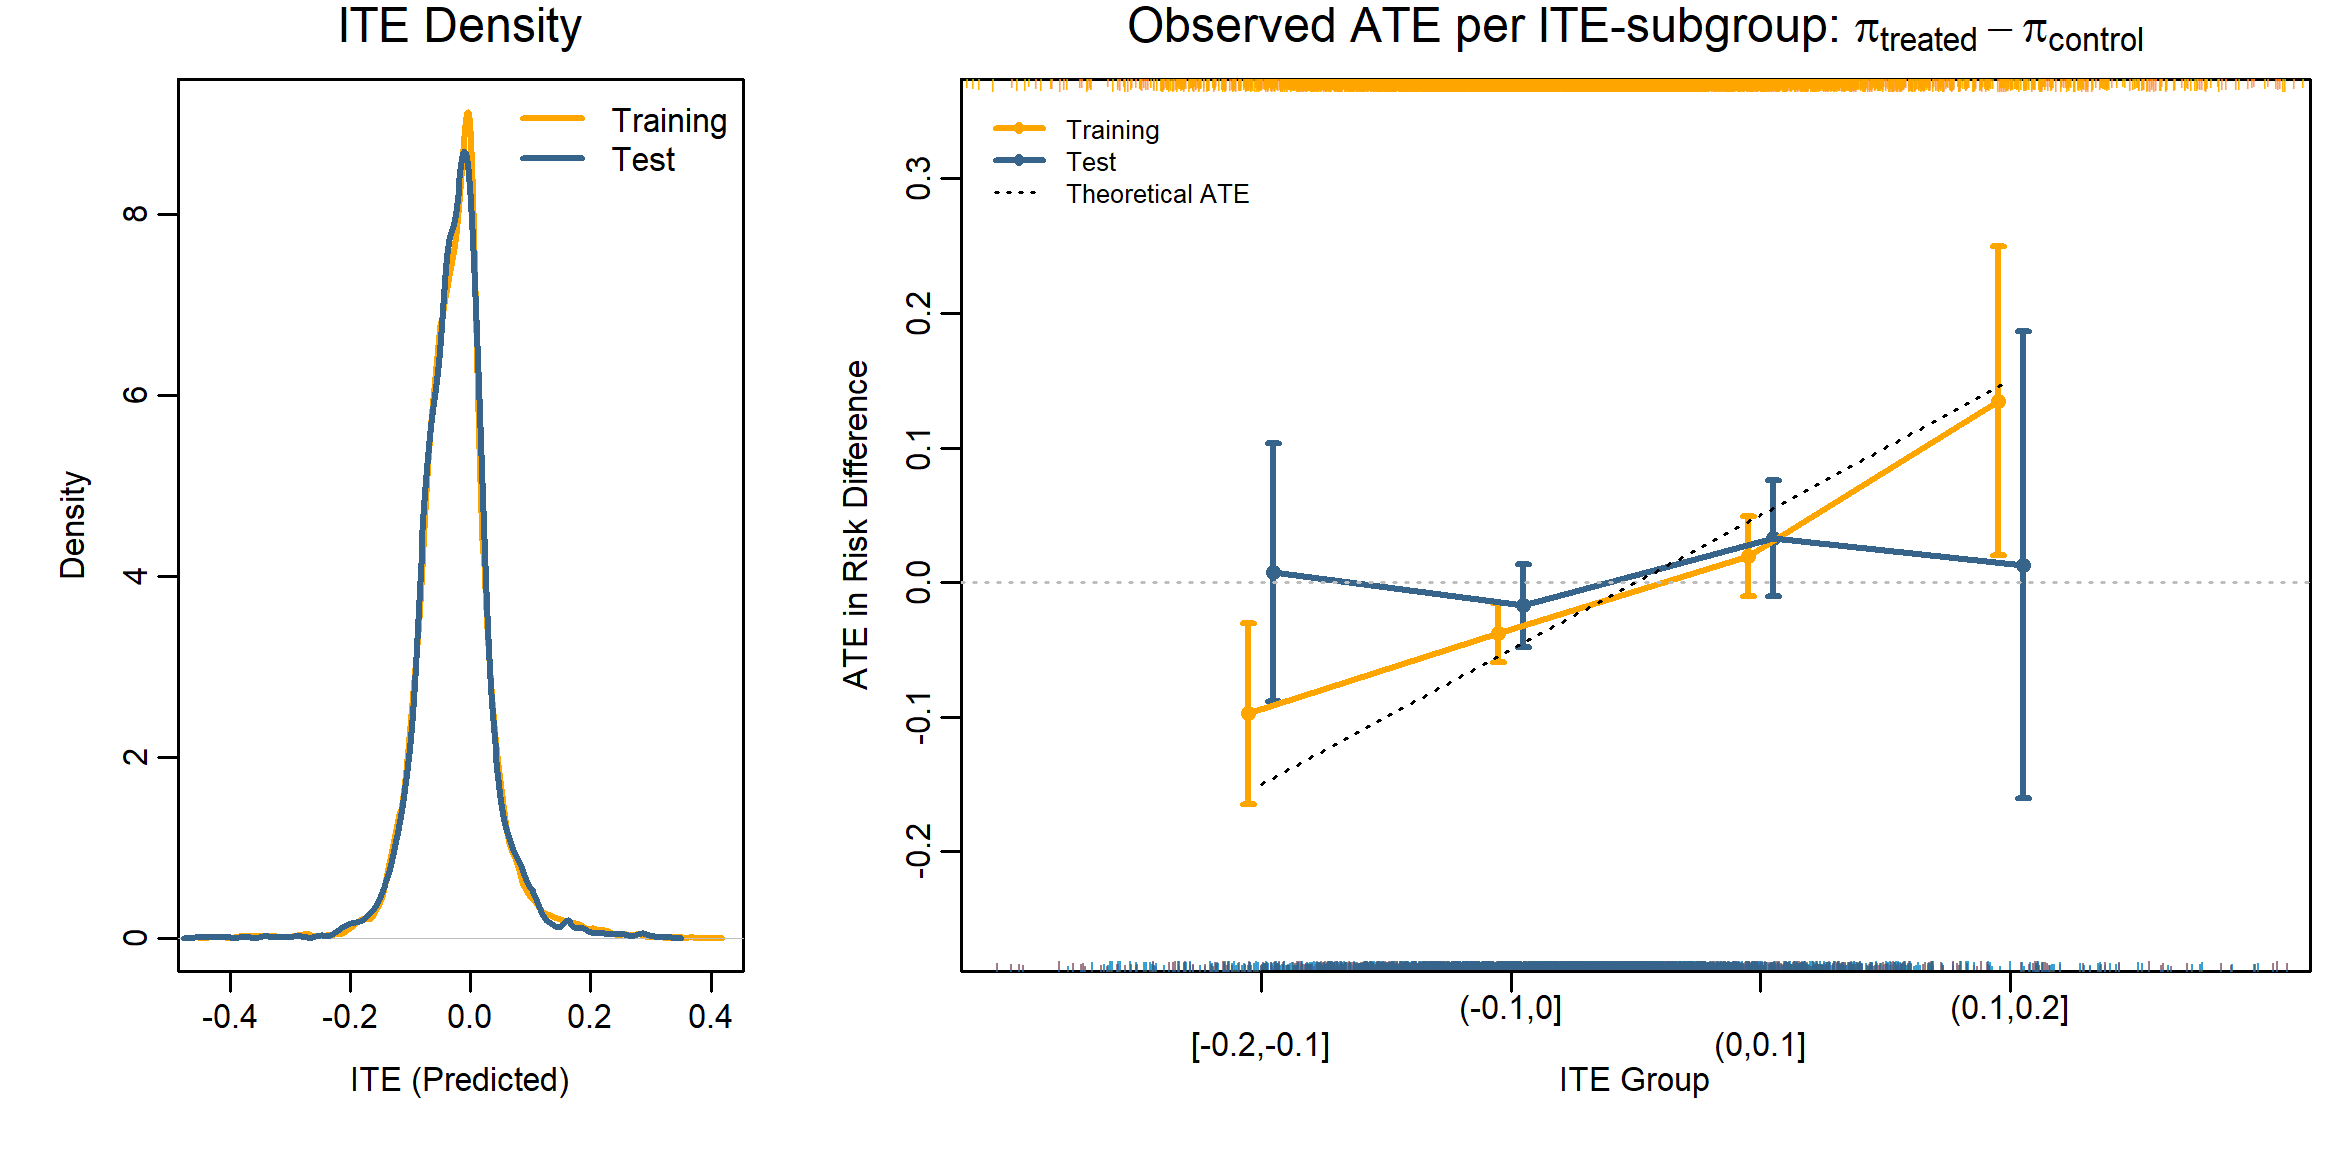
\includegraphics[width=0.9\textwidth]{img/results_IST/glm_tlearner_density_ITE_ATE.png}
\caption{Results for the International Stroke Trial (IST) using the T-learner logistic regression. Left: density of predicted ITEs in the training and test sets; Right: observed ATE in terms of risk difference per estimated ITE subgroup.}
\label{fig:IST_density_ITE_ATE_glm_tlearner}
\end{figure}



\begin{figure}[htbp]
\centering
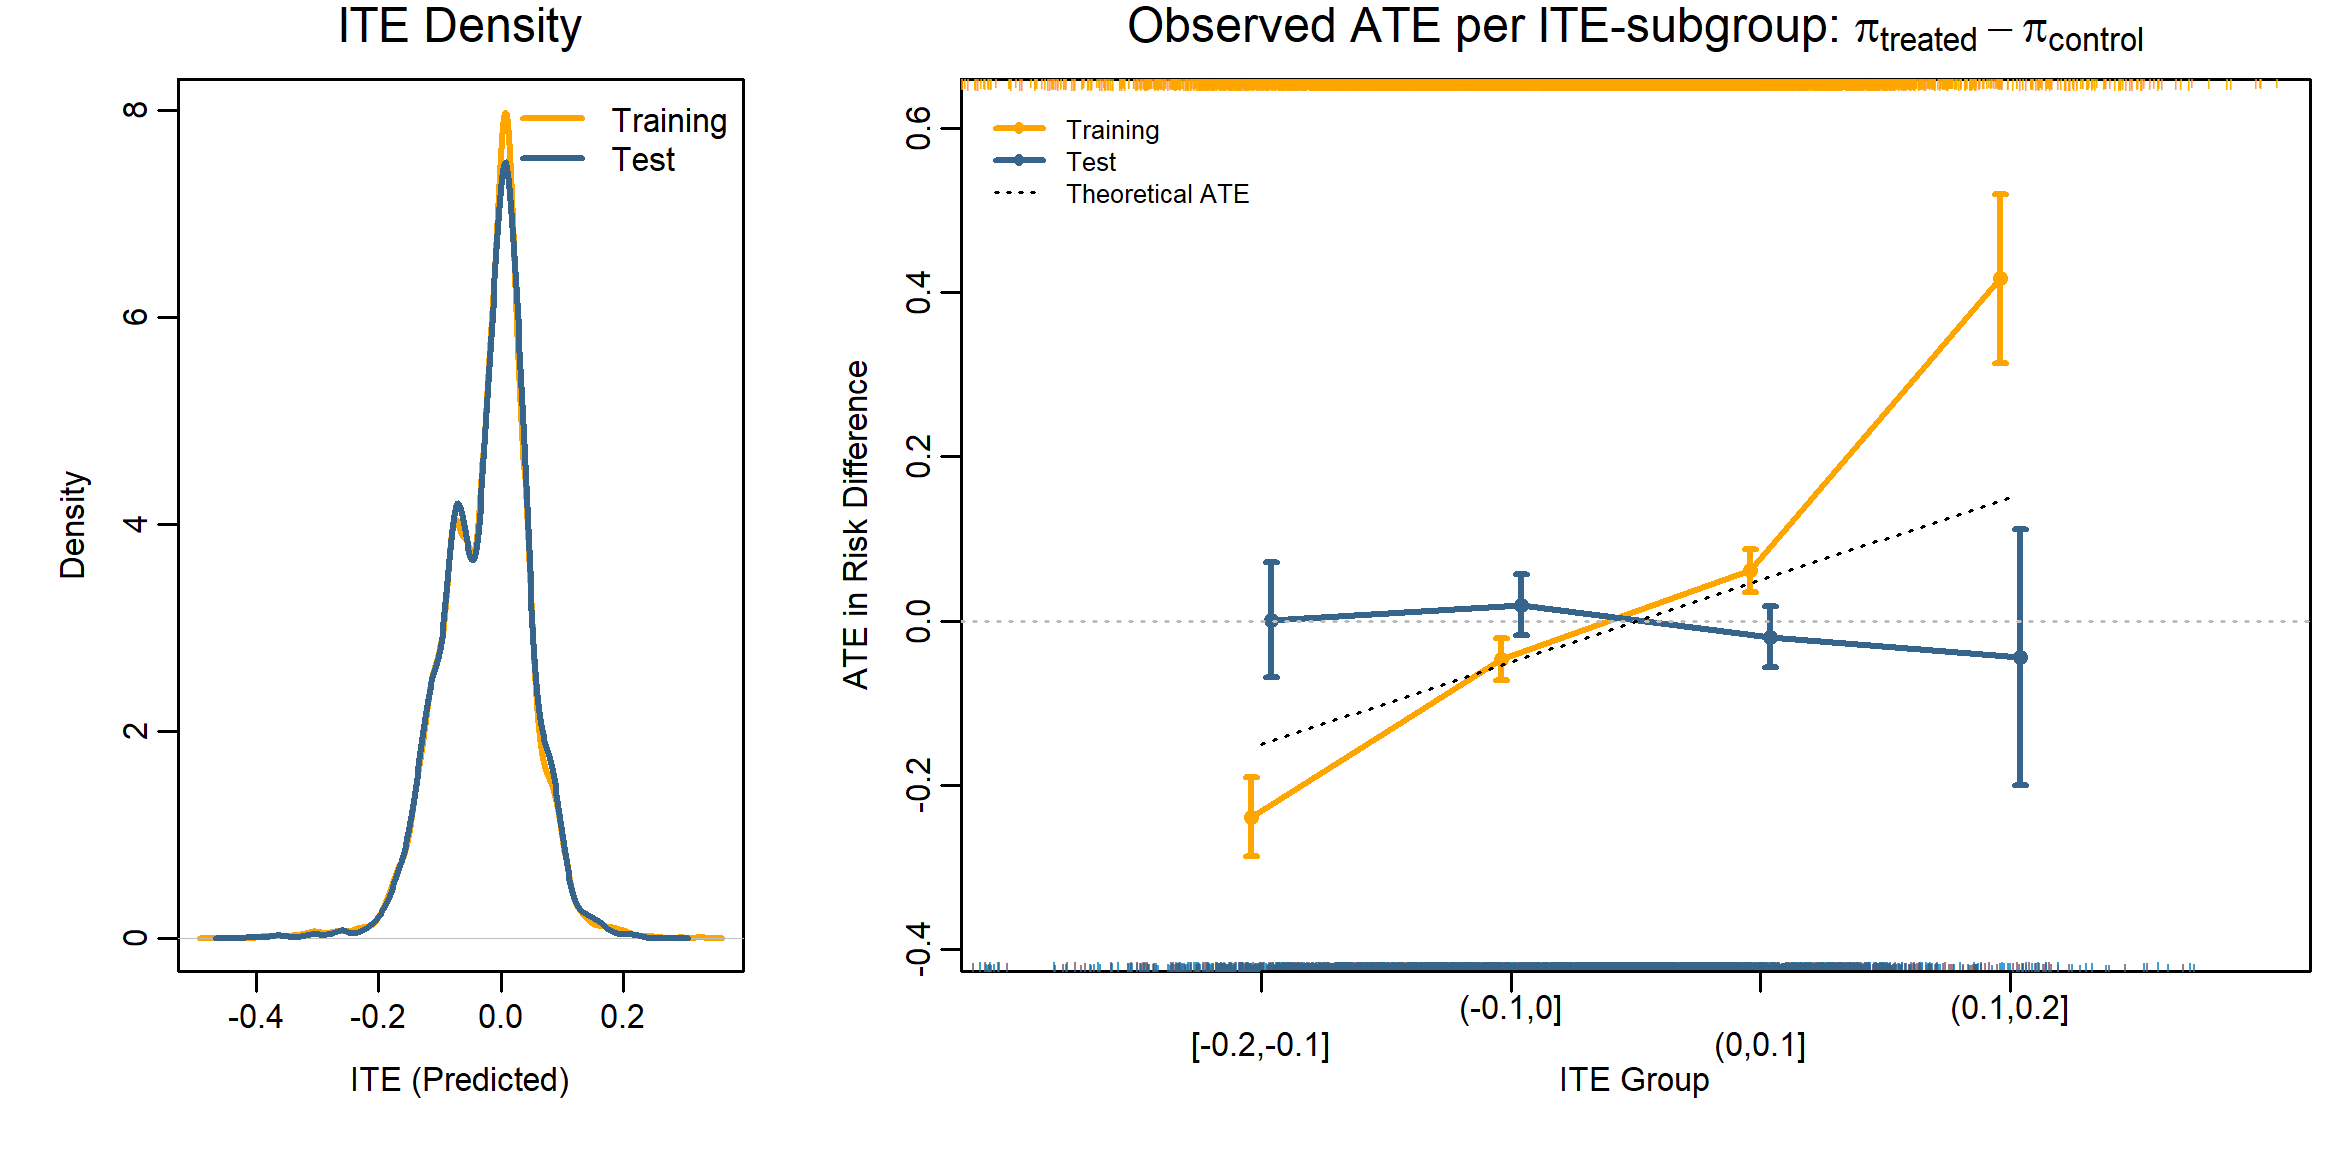
\includegraphics[width=0.9\textwidth]{img/results_IST/IST_tuned_rf_tlearner_density_ITE_ATE.png}
\caption{Results for the International Stroke Trial (IST) using the T-learner tuned random forest. Left: density of predicted ITEs in the training and test sets; Right: observed ATE in terms of risk difference per estimated ITE subgroup.}
\label{fig:IST_density_ITE_ATE_tuned_rf}
\end{figure}


\begin{figure}[htbp]
\centering
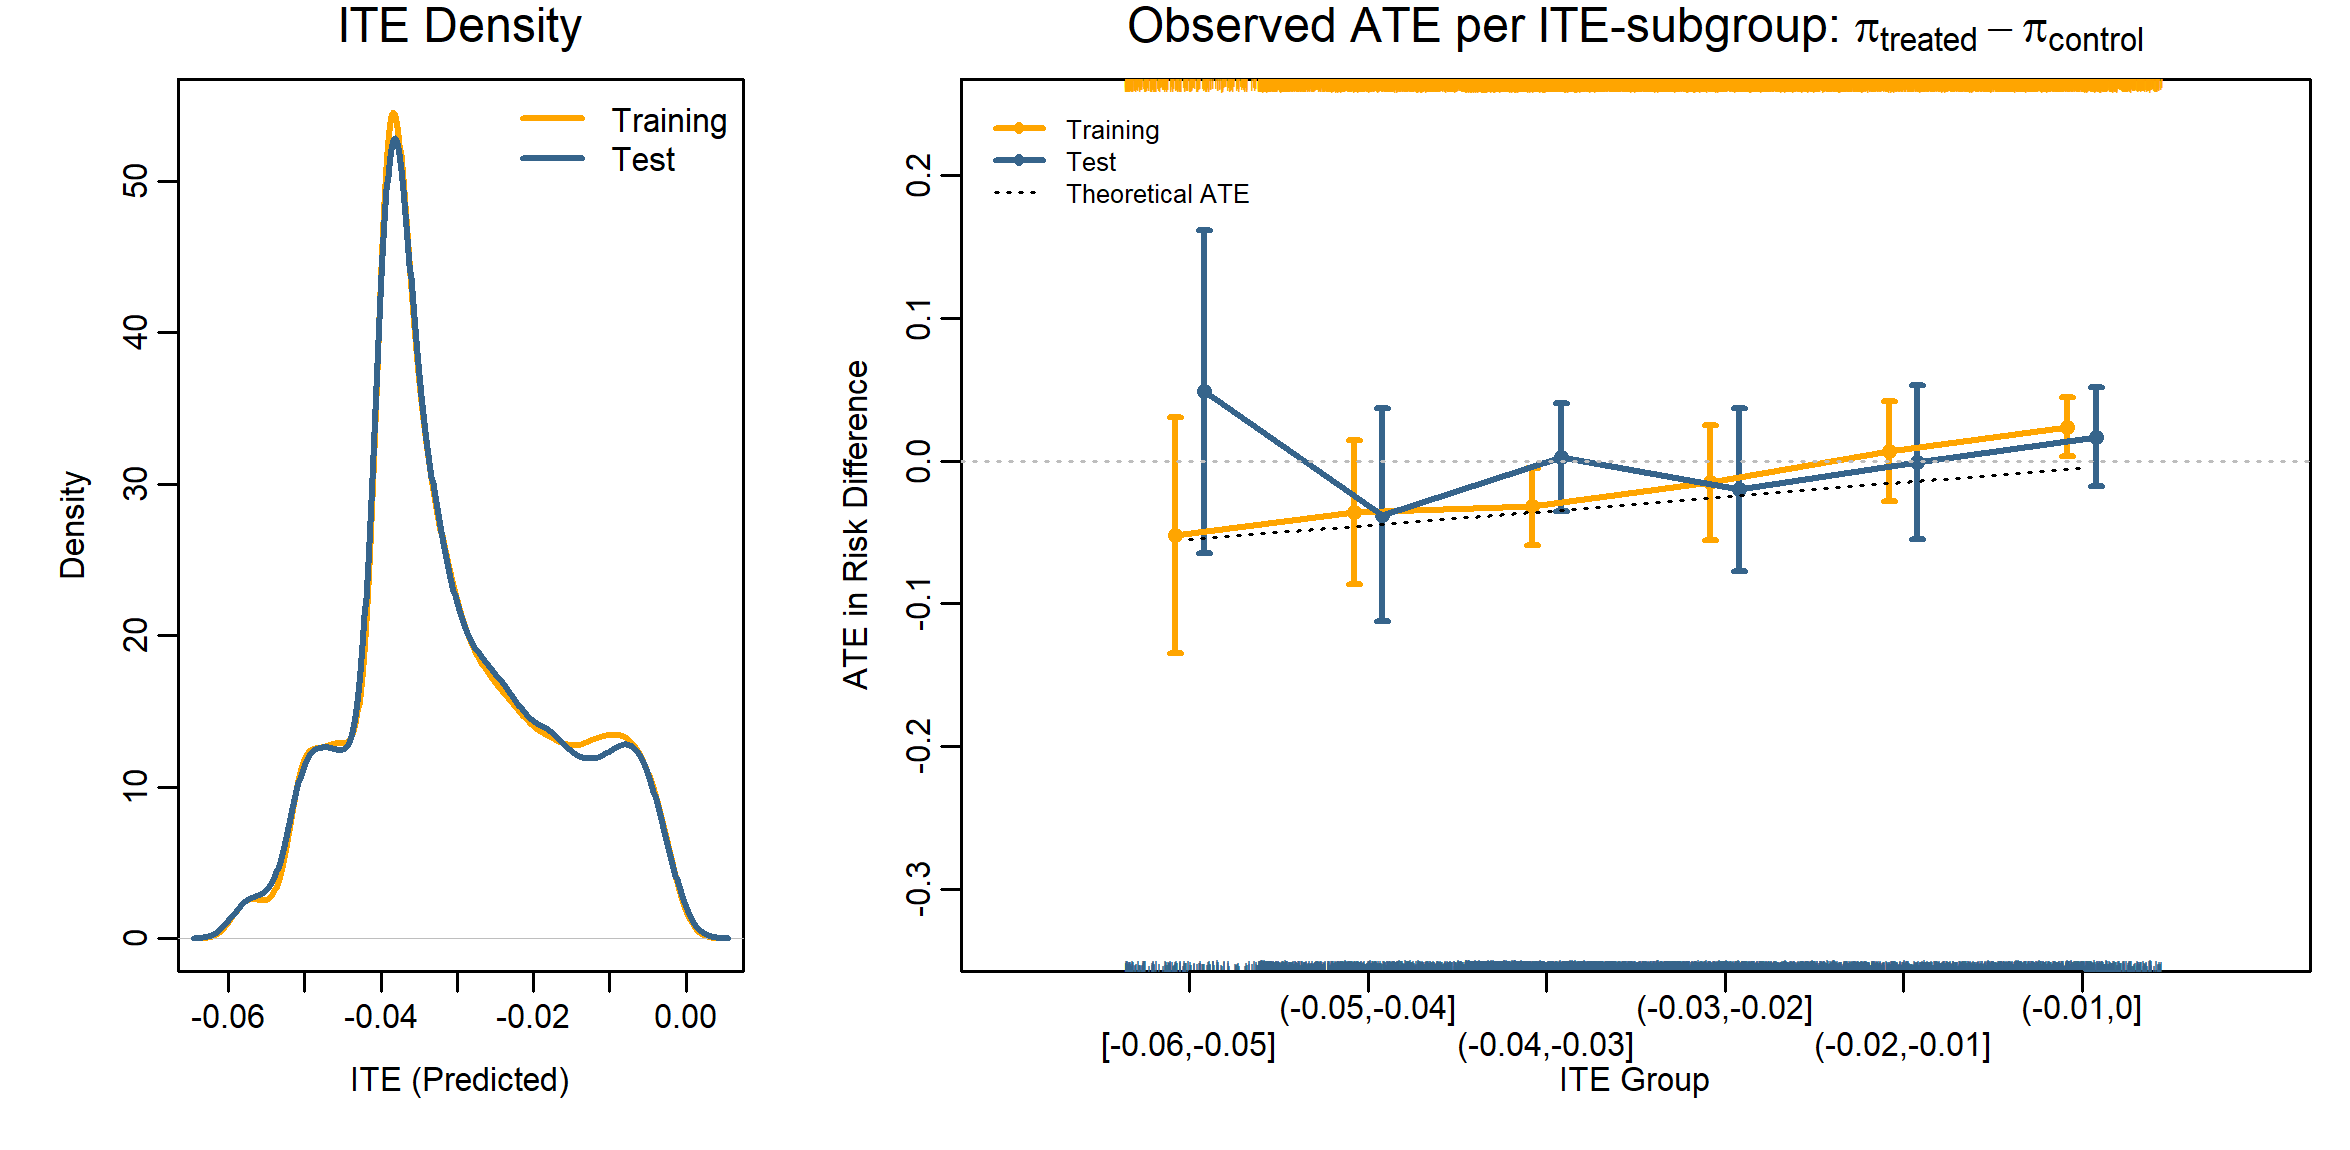
\includegraphics[width=0.9\textwidth]{img/results_IST/IST_TRAM_DAG_slearner_density_ITE_ATE.png}
\caption{Results for the International Stroke Trial (IST) using the S-learner TRAM-DAG. Left: density of predicted ITEs in the training and test sets; Right: observed ATE in terms of risk difference per estimated ITE subgroup.}
\label{fig:IST_density_ITE_ATE_TRAM_DAG}
\end{figure}




% enforce that starts after all floats have been displayed
\FloatBarrier

\section{Discussion}

We observed similar results to those reported by \citet{chen2025} when estimating ITEs on the International Stroke Trial dataset across all three models: the T-learner logistic regression, the T-learner tuned random forest, and the S-learner TRAM-DAG. The logistic model showed moderate discrimination in the training set, which did not generalize to the test set, as illustrated by the ITE-ATE plot in Figure~\ref{fig:IST_density_ITE_ATE_glm_tlearner}. The tuned random forest model showed stronger discrimination in the training set but similarly failed to generalize to the test set (Figure~\ref{fig:IST_density_ITE_ATE_tuned_rf}). In contrast, the S-learner TRAM-DAG estimated less heterogeneity than the other two models, as shown in the density plot in Figure~\ref{fig:IST_density_ITE_ATE_TRAM_DAG}, resulting in weak discrimination in both the training and test sets. For all three models, the confidence intervals in the ITE-ATE plots on the test set included the zero line, suggesting no significant effect in any of the estimated ITE subgroups.

\medskip


Poor calibration does not appear to explain the limited ITE performance, as calibration on the test set was good, as shown in Appendix~\ref{sec:calibrations_experiment2}, Figures~\ref{fig:calibration_IST_glm}-\ref{fig:calibration_IST_TRAM_DAG}. However, since the ground truth is unknown, it remains unclear whether the models fail to detect true treatment effect heterogeneity, or whether the heterogeneity is too small, or driven by unobserved effect modifiers. We investigate these possibilities further in Experiment 3, Chapter~\ref{ch:experiment3}.




%%%%%%%%%%%%%%%%%%%%%%%%%%%%%%%%%%%%%%%%%%%%%%%%%%%%%%%%%%%%%%%%%%%%%%
%%%%%%%%%%%%%%%%%%%%%%%%%%%%%%%%%%%%%%%%%%%%%%%%%%%%%%%%%%%%%%%%%%%%%%

% 

% LaTeX file for Chapter Exp3




\chapter{Experiment 3: ITE model robustness in RCTs (simulation)} \label{ch:experiment3}




\section{Motivation}

In this section, we perform a simulation study to estimate the ITE using different models in an RCT setting under various scenarios. The aim is to identify conditions under which ITE estimation fails, and whether such failure is model-agnostic -- i.e., driven by external factors such as unobserved covariates or the strength of the treatment effect, rather than by the model class itself. This may provide insight into why ITE estimation can fail in real-world applications, as demonstrated by \citet{chen2025} on the IST dataset and replicated in our own work in Experiment 2 (Section~\ref{sec:results_experiment2}). 


\section{Setup} \label{sec:methods_experiment3}

The simulation is based on a data-generating process (DGP) that resembles an RCT. We assume a binary outcome and a set of covariates that influence the outcome. There may also be treatment-covariate interactions that are responsible for heterogeneity in the treatment effect.

\medskip

\textbf{Data-generating process:} Data is generated similarly to the approach proposed by \citet{hoogland2021}. The binary treatment ($T$) is sampled from a Bernoulli distribution with probability 0.5. The five covariates ($\mathbf{X}$), representing patient-specific characteristics at baseline, are drawn from a multivariate standard normal distribution with a compound symmetric covariance matrix ($\rho=0.1$). The binary outcome ($Y$) is sampled from a Bernoulli distribution with probability $\text{P}(Y_i = 1 \mid  \mathbf{X_i} = \mathbf{x_i}, T_i = t_i) = \text{logit}^{-1} \left(\beta_0 + \beta_T t_i + \boldsymbol{\beta}_X^\top \mathbf{x_i} + t_i \cdot \boldsymbol{\beta}_{TX}^\top \mathbf{x_{TX,i}} \right)$, where $i$ denotes the patient index, and $\mathbf{x}_{TX,i}$ denotes the subset of covariates that interact with the treatment.

The simulated datasets are generated under three scenarios, where coefficients are set to different values or not all variables are observed. In Scenario 1, the coefficients are: $\beta_0 = 0.45$ (intercept), $\beta_T = -0.85$ (direct treatment effect), $\boldsymbol{\beta}_X = (-0.5, 0.8, 0.2, 0.6, -0.4)$ (direct covariate effects), and $\boldsymbol{\beta}_{TX} = (0.9, 0.1)$ (interaction effects between treatment and covariates $X_1$ and $X_2$ on the outcome). In Scenario 2, the same coefficients are used, but the covariate $X_1$, which is responsible for a large portion of the heterogeneity, is not observed in the final dataset. This is expected to cause difficulties in estimating the ITE. In Scenario 3, the coefficients for the direct treatment and interaction effects are set to $\beta_T = -0.05$ and $\boldsymbol{\beta}_{TX} = (-0.01, 0.03)$ to represent a weak treatment effect and low heterogeneity. All other coefficients remain unchanged, and all covariates are observed. The DAGs corresponding to the three scenarios are presented in Figure~\ref{fig:simulation_dags}.


% here include 3 figures side by side 
% /img/results_ITE_simulation/simulation_observed.png
% simulation_unobserved.png
% simulation_small_effects.png

\begin{figure}[H]
\centering
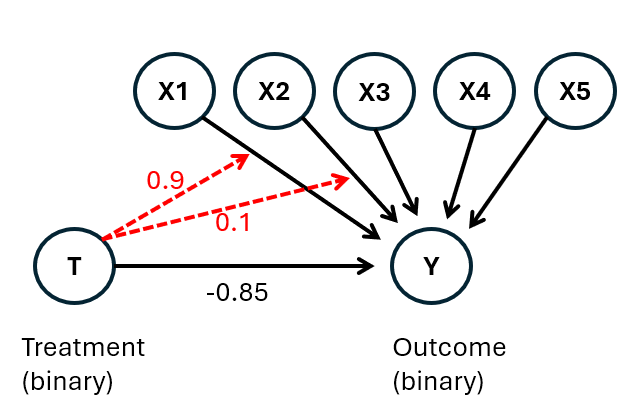
\includegraphics[width=0.3\textwidth]{img/results_ITE_simulation/simulation_observed.png}
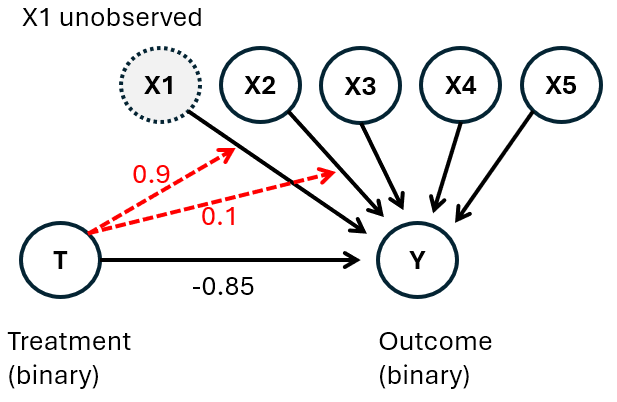
\includegraphics[width=0.3\textwidth]{img/results_ITE_simulation/simulation_unobserved.png}
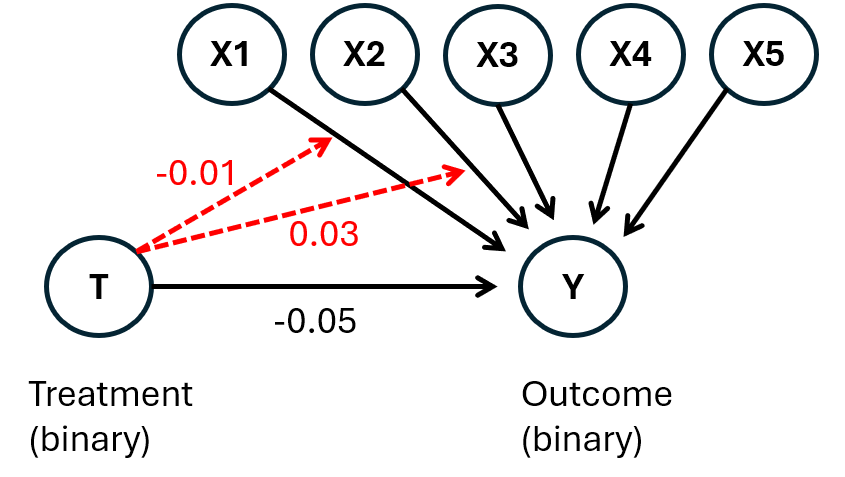
\includegraphics[width=0.3\textwidth]{img/results_ITE_simulation/simulation_small_effects.png}
\caption{Data-generating process (DGP) for the three scenarios in the ITE simulation study (RCT). Interaction effects between treatment ($T$) and covariates ($X_1$ and $X_2$) on the outcome ($Y$) are shown in red. Left: Scenario 1, where all covariates are observed and both treatment effect and heterogeneity are strong; Middle: Scenario 2, with the same DGP as in Scenario 1, but where covariate $X_1$ is not observed; Right: Scenario 3, where the treatment effect and heterogeneity are weak, and all covariates are observed.}
\label{fig:simulation_dags}
\end{figure}




% The data is generated for three different scenarios, where the coefficients are set to different values to represent different treatment effects and interaction effects and by removing the covariate $X1$ from the final dataset in scenario 2, hence making it unobserved. The scenarios are summarized in Table \ref{tab:simulation_scenarios}.


% Table with szenarios:

% Szenario 1: 
% description: strong direct and interaction effect of treatment, fully observed
% coefficients: \beta_0 = 0.45, \beta_T = -0.85,  \boldsymbol{\beta}_X = c(-0.5, 0.8, 0.2, 0.6, -0.4), \boldsymbol{\beta}_{TX} = c(0.9, 0.1)
% motivation: this scenario should represent the ideal case where there is high heterogeneity and all variables are observed, hence the ITE estimation is assumed to work well.

% Szenario 2:
% description: strong direct and interaction effect of treatment, but covariate X1 not observed
% coefficients: \beta_0 = 0.45, \beta_T = -0.85,  \boldsymbol{\beta}_X = c(-0.5, 0.8, 0.2, 0.6, -0.4), \boldsymbol{\beta}_{TX} = c(0.9, 0.1)
% motivation: removing the covariate X1, which is responsible for much of the heterogeneity, should cause difficulties in ITE estimation because the heterogeneity can not be attributed to the right covariate.

% Szenario 3:
% description: weak direct and interaction effect of treatment, fully observed
% coefficients: \beta_0 = 0.45, \beta_T = -0.05,  \boldsymbol{\beta}_X = c(-0.5, 0.8, 0.2, 0.6, -0.4), \boldsymbol{\beta}_{TX} = c(-0.01, 0.03)
% motivation: this scenario should represent the case where the treatment effect is weak and heterogeneity is low, hence the model should estimate only small range of ITE.





% \subsubsection*{Scenario 1: Strong effects, all covariates observed}
% 
% This scenario represents an ideal case in which the treatment has a strong direct and interaction effect. All covariates are observed, supposedly enabling effective ITE estimation. The coefficients are set as follows:
% 
% 
% 
% % X1 and X2 interact with treatment
% \begin{align*}
%     \beta_0 &= 0.45,\quad \beta_T = -0.85, \\
%     \boldsymbol{\beta}_X &= (-0.5,\ 0.8,\ 0.2,\ 0.6,\ -0.4), \\
%     \boldsymbol{\beta}_{TX} &= (0.9,\ 0.1) , X_1 \text{ and } X_2 \text{ interact with treatment}
% \end{align*}
% 
% \vspace{0.5em}
% 
% \subsubsection*{Scenario 2: Strong effects, covariate \boldmath$X_1$ unobserved}
% 
% This scenario uses the same coefficients as Scenario 1, but with covariate $X_1$ removed from the dataset. As $X_1$ drives a large portion of the treatment effect heterogeneity, the estimation of the ITE is expected to be biased or incomplete when $X_1$ is not observed.
% 
% 
% \begin{align*}
%     \beta_0 &= 0.45,\quad \beta_T = -0.85, \\
%     \boldsymbol{\beta}_X &= (-0.5,\ 0.8,\ 0.2,\ 0.6,\ -0.4), \\
%     \boldsymbol{\beta}_{TX} &= (0.9,\ 0.1) , X_1 \text{ and } X_2 \text{ interact with treatment}
% \end{align*}
% \textit{Note: $X_1$ is not included in the final dataset.}
% 
% \vspace{0.5em}
% 
% \subsubsection*{Scenario 3: Weak Effects, All Covariates Observed}
% 
% This scenario illustrates a setting with minimal treatment effect and weak treatment-covariate interaction. While all covariates are observed, the model is expected to recover only low-variance ITEs due to limited signal.
% 
% \begin{align*}
%     \beta_0 &= 0.45,\quad \beta_T = -0.05, \\
%     \boldsymbol{\beta}_X &= (-0.5,\ 0.8,\ 0.2,\ 0.6,\ -0.4), \\
%     \boldsymbol{\beta}_{TX} &= (-0.01,\ 0.03), X_1 \text{ and } X_2 \text{ (weakly) interact with treatment}
% \end{align*}


\textbf{Models for ITE estimation:} We applied the following models in \texttt{R} to estimate individualized treatment effects (ITEs): T-learner logistic regression (\texttt{stats} package), T-learner and S-learner logistic lasso regression (\texttt{glmnet} package \citep{friedman2010}, with $\lambda$ selected via 10-fold cross-validation), T-learner random forest (\texttt{randomForest} package \citep{breiman2001}, 100 trees), and T-learner tuned random forest (\texttt{comets} package \citep{comets}, which tunes \texttt{mtry} and \texttt{max.depth} using out-of-bag error, 500 trees).

While all models were run, we focus on two for the main results: the T-learner logistic regression as a baseline (matching the DGP), and the tuned random forest as a more flexible non-parametric model. Results for the default random forest in Scenario 1 are shown in Appendix~\ref{sec:default_rf_ite} to highlight the role of model tuning in avoiding overfitting and ensuring proper calibration.

Each model was trained and evaluated on independent datasets of 10,000 samples generated from the same DGP. Although TRAM-DAGs are well suited for ITE estimation, we did not include them here, as the goal of this experiment is to compare simpler and more complex models under varying conditions. TRAM-DAGs are evaluated in other experiments in this thesis.
% 
% 
% \textbf{Models for ITE estimation:} We applied the following models in \texttt{R} to estimate the ITEs: T-learner logistic regression (\texttt{stats} package), T-learner logistic lasso regression (\texttt{glmnet} package \citep{friedman2010}, with the regularization parameter $\lambda$ estimated via 10-fold cross-validation), S-learner logistic lasso regression (same as the T-learner), T-learner random forest (\texttt{randomForest} package \citep{breiman2001}, 100 trees), and T-learner tuned random forest (\texttt{comets} package \citep{comets}, which tunes the number of variables considered for splitting at each node (\texttt{mtry}) and the maximum tree depth (\texttt{max.depth}) using out-of-bag error, 500 trees). 
% 
% While all models were applied, we present only the results of the T-learner logistic regression as a benchmark (same model as used in the data-generating process), and the tuned random forest as representation of a complex non-parametric model. In Appendix~\ref{sec:default_rf_ite}, we additionally present the results for a standard random forest evaluated for Scenario 1 to illustrate the importance of model tuning to prevent overfitting and ensure accurate calibration.
% 
% All models were trained on a training set and evaluated on a test set, each consisting of 10,000 samples generated from the same DGP. TRAM-DAGs would also be well suited for ITE estimation in this setting, but we chose not to apply them in this experiment, since the main objective is to assess behavioral differences between complex and simple models under different scenarios. TRAM-DAGs are applied in other experiments in this thesis.

\medskip

\textbf{Model evaluation:} Model performance is evaluated visually on both the training and test datasets. For predictive performance, we present true vs. predicted probabilities $\text{P}(Y = 1 \mid X, T)$ to assess how well each model is calibrated. Plots of true vs. predicted ITEs show how closely the model estimates match the true effects. Since the true probabilities and ITEs are known by design in this simulation, direct evaluation of calibration and prediction accuracy is possible, unlike in real-world applications.

To assess whether estimated ITEs correspond to actual observed outcomes, we use ITE-ATE plots. These show the observed average treatment effect (ATE), calculated as $\text{P}(Y = 1 \mid T = 1) - \text{P}(Y = 1 \mid T = 0)$, in the respective subgroups of estimated ITEs. Accurate models should produce ITE-ATE points that align with the identity line.

These simulation scenarios allow us to assess ITE estimation performance under challenging conditions such as omitted variables and weak treatment effects. The subsequent results reveal which models remain robust under such violations and provide insight into possible real-world estimation failures.




\section{Results} \label{sec:results_experiment3}

In this section, we present the performance of two causal machine learning models -- T-learner logistic regression and T-learner tuned random forest -- for estimating ITEs under the three simulated scenarios introduced in Section~\ref{sec:methods_experiment3}. Scenario~(1) represents the ideal case where all covariates are observed and both treatment and interaction effects are strong. In Scenario~(2), a key effect modifier is unobserved, and in Scenario~(3), treatment and interaction effects are weak, but all covariates are observed.

Results for all scenarios are presented in Figures~\ref{fig:fully_observed_glm_tlearner} to~\ref{fig:small_interaction_tuned_rf_tlearner}.



\subsection{Scenario (1): Fully observed, large effects}



\begin{figure}[htbp]
\centering
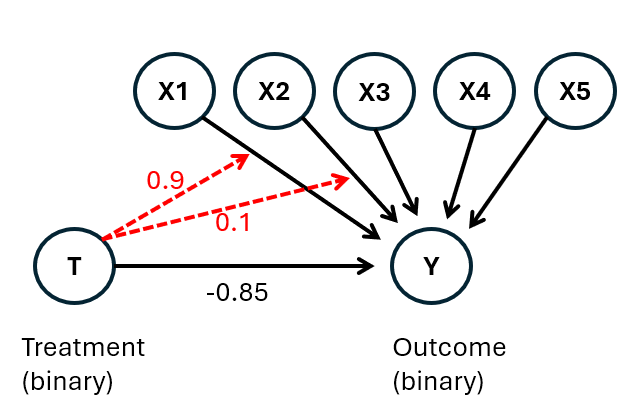
\includegraphics[width=0.35\textwidth]{img/results_ITE_simulation/simulation_observed.png}
\caption{DAG for Scenario~(1), where all variables are observed and both treatment and interaction effects are strong. This DAG was previously shown in Figure~\ref{fig:simulation_dags} and is re-plotted here for convenience. The numbers indicate the coefficients on the log-odds scale. Red arrows represent interaction effects between treatment ($T$) and covariates ($X_1$ and $X_2$) on the outcome ($Y$).}
\label{fig:fully_observed_dag}
\end{figure}


\begin{figure}[htbp]
\centering
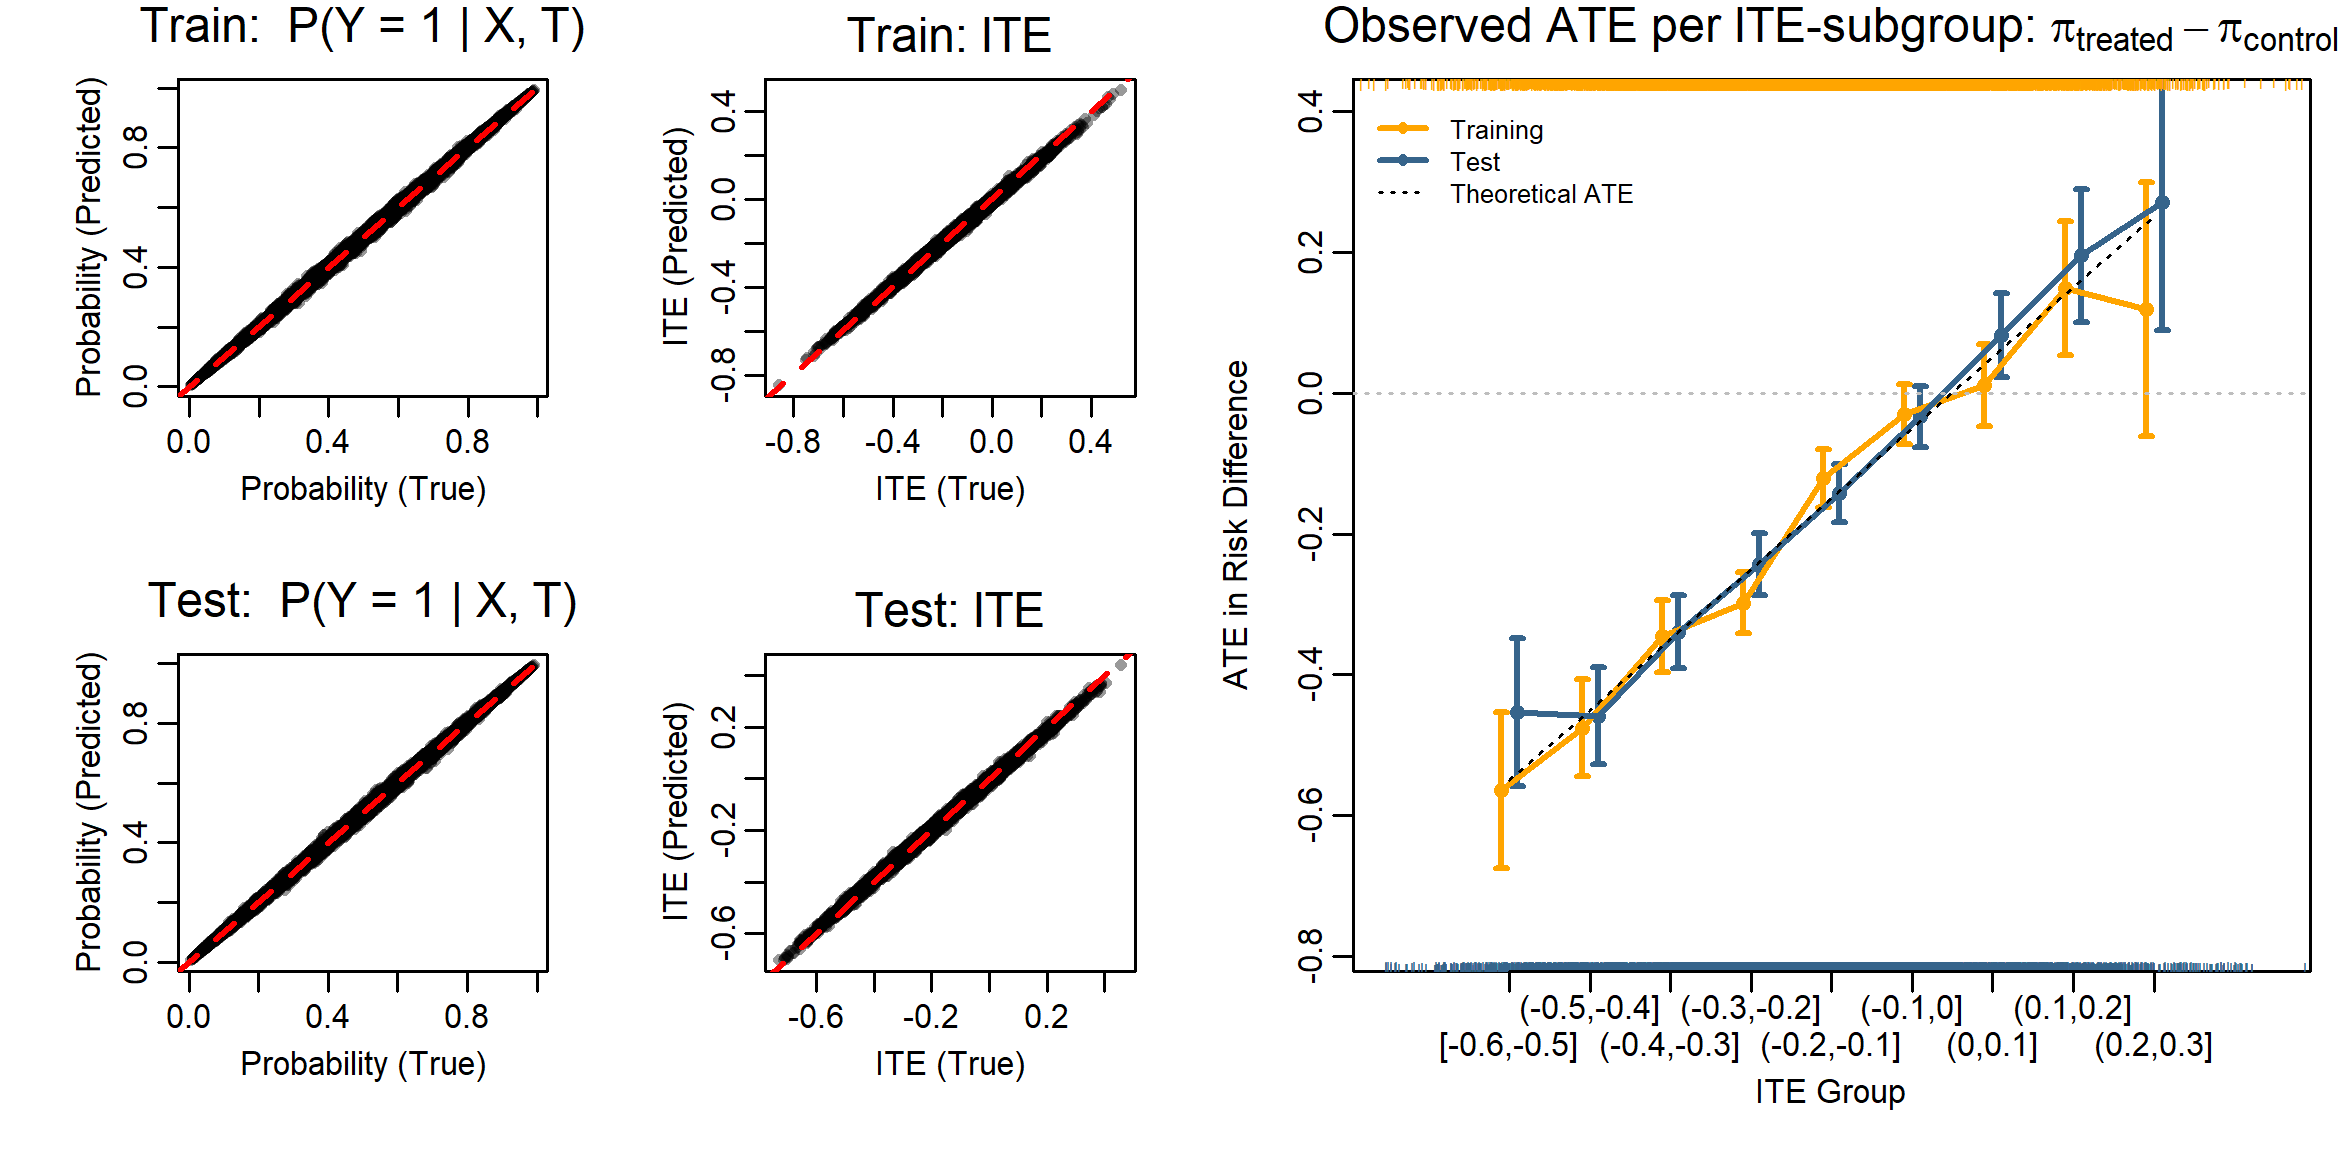
\includegraphics[width=0.9\textwidth]{img/results_ITE_simulation/fully_observed_glm_tlearner.png}
\caption{Results of the T-learner logistic regression in Scenario~(1), where the DAG is fully observed and both treatment and interaction effects are strong. Left: true vs. predicted probabilities for $\text{P}(Y = 1 \mid X, T)$; Middle: true vs. predicted ITEs; Right: observed ATE in terms of risk difference per estimated ITE subgroup.}
\label{fig:fully_observed_glm_tlearner}
\end{figure}


\begin{figure}[htbp]
\centering
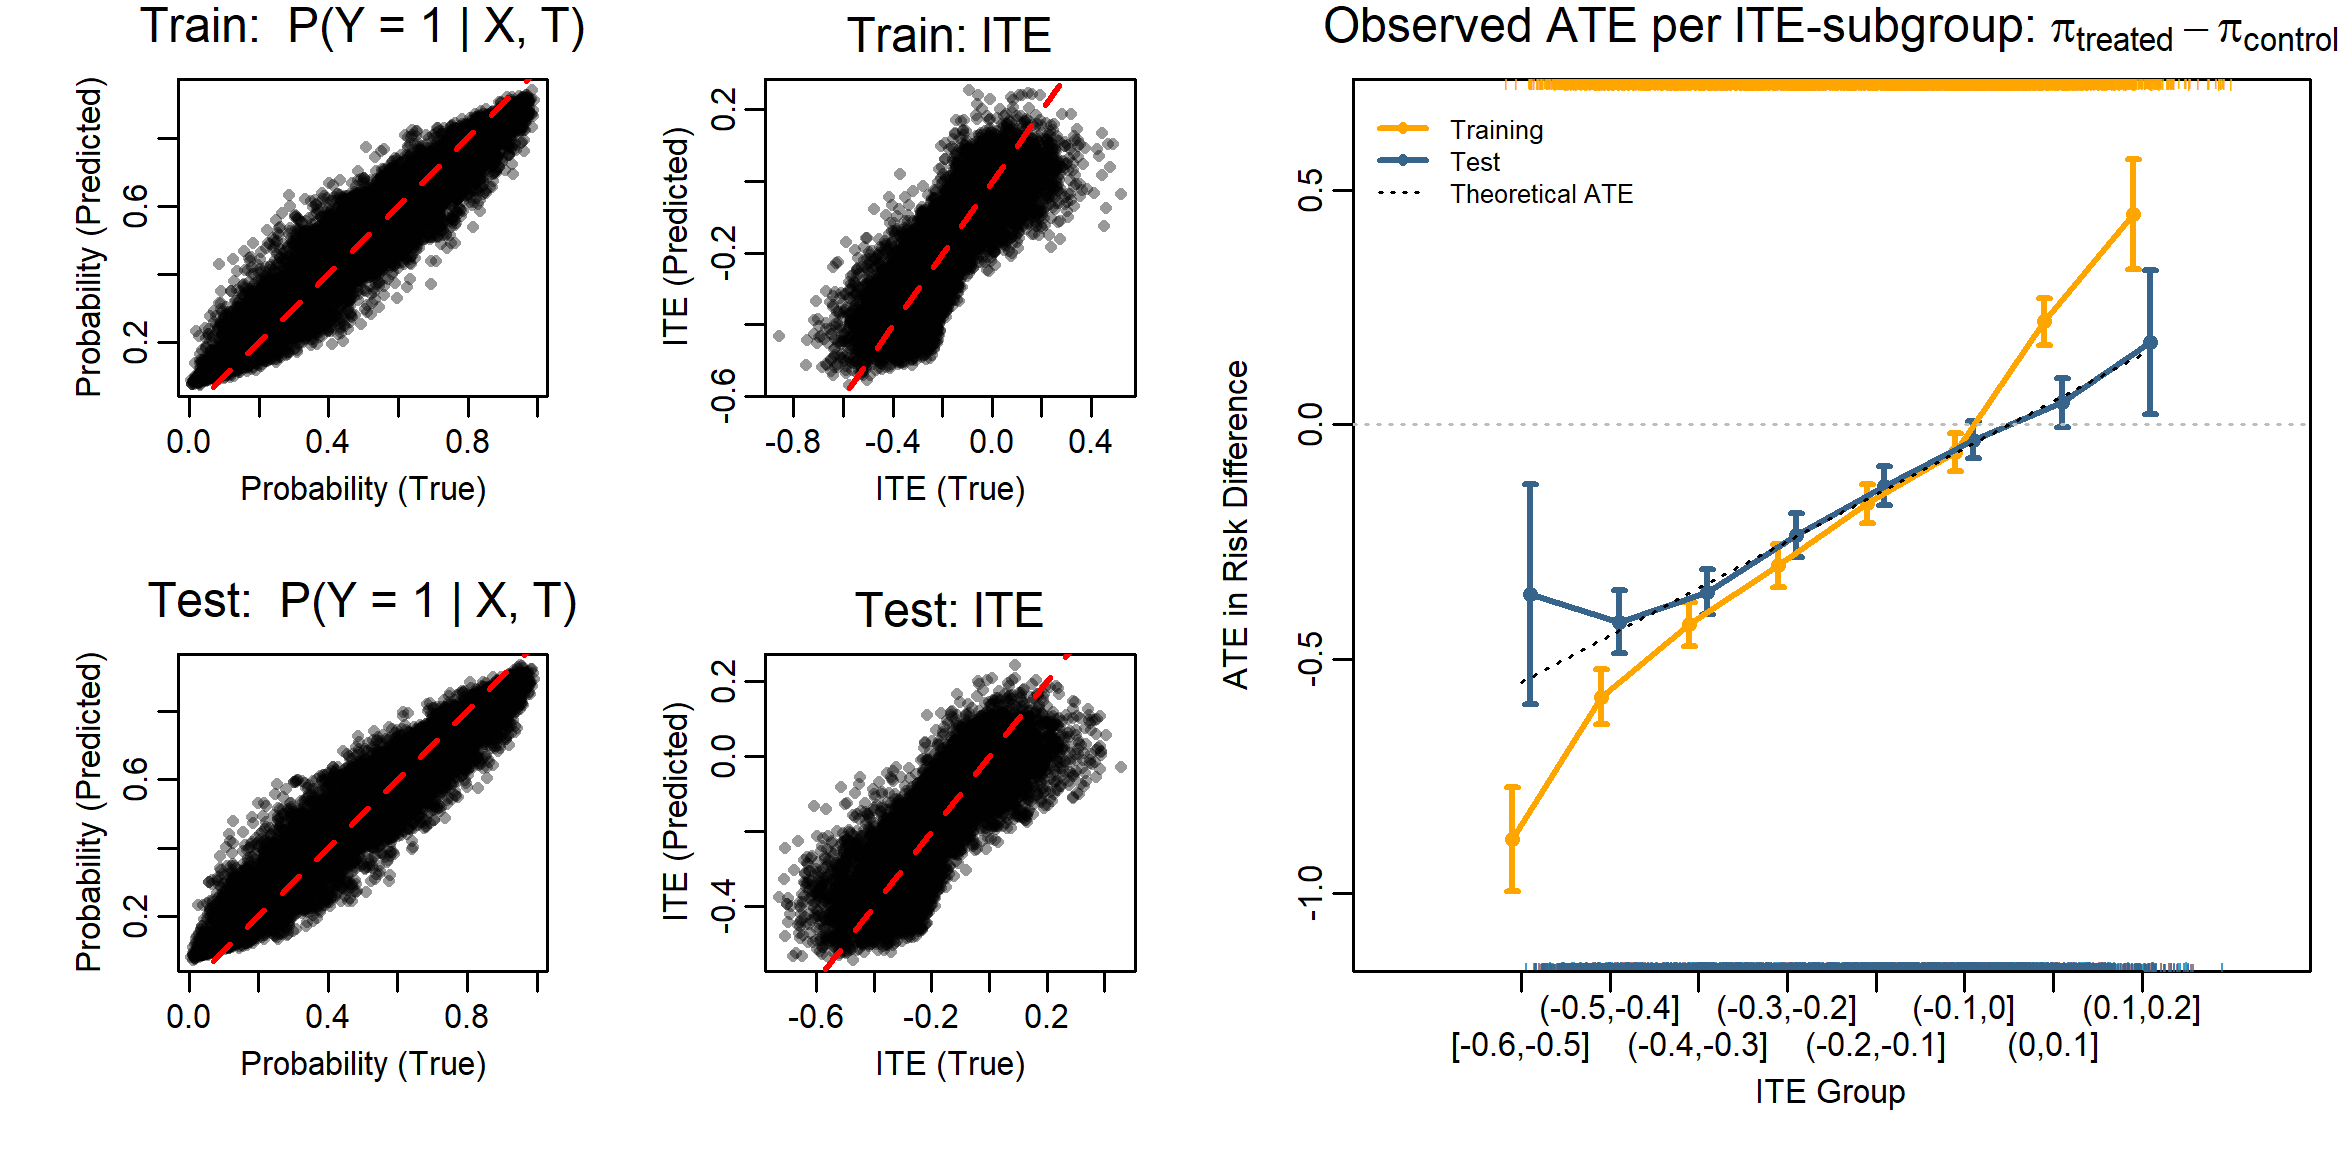
\includegraphics[width=0.9\textwidth]{img/results_ITE_simulation/fully_observed_tuned_rf_tlearner.png}
\caption{Results of the T-learner tuned random forest in Scenario~(1), where the DAG is fully observed and both treatment and interaction effects are strong. Left: true vs. predicted probabilities for $\text{P}(Y = 1 \mid X, T)$; Middle: true vs. predicted ITEs; Right: observed ATE in terms of risk difference per estimated ITE subgroup.}
\label{fig:fully_tuned_rf_tlearner}
\end{figure}


\clearpage



\subsection{Scenario (2): Unobserved interaction}

\begin{figure}[htbp]
\centering
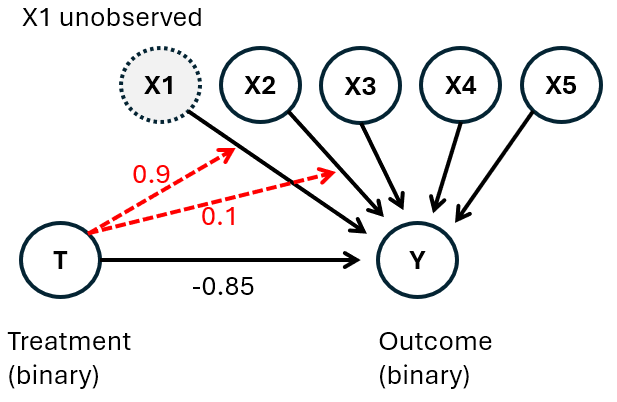
\includegraphics[width=0.35\textwidth]{img/results_ITE_simulation/simulation_unobserved.png}
\caption{DAG for Scenario~(2), where there are strong treatment and interaction effects, but variable $X_1$ is not observed. This DAG was previously shown in Figure~\ref{fig:simulation_dags} and is re-plotted here for convenience. The numbers indicate the coefficients on the log-odds scale. Red arrows represent interaction effects between treatment ($T$) and covariates ($X_1$ and $X_2$) on the outcome ($Y$).}
\label{fig:unobserved_interaction_dag}
\end{figure}



\begin{figure}[htbp]
\centering
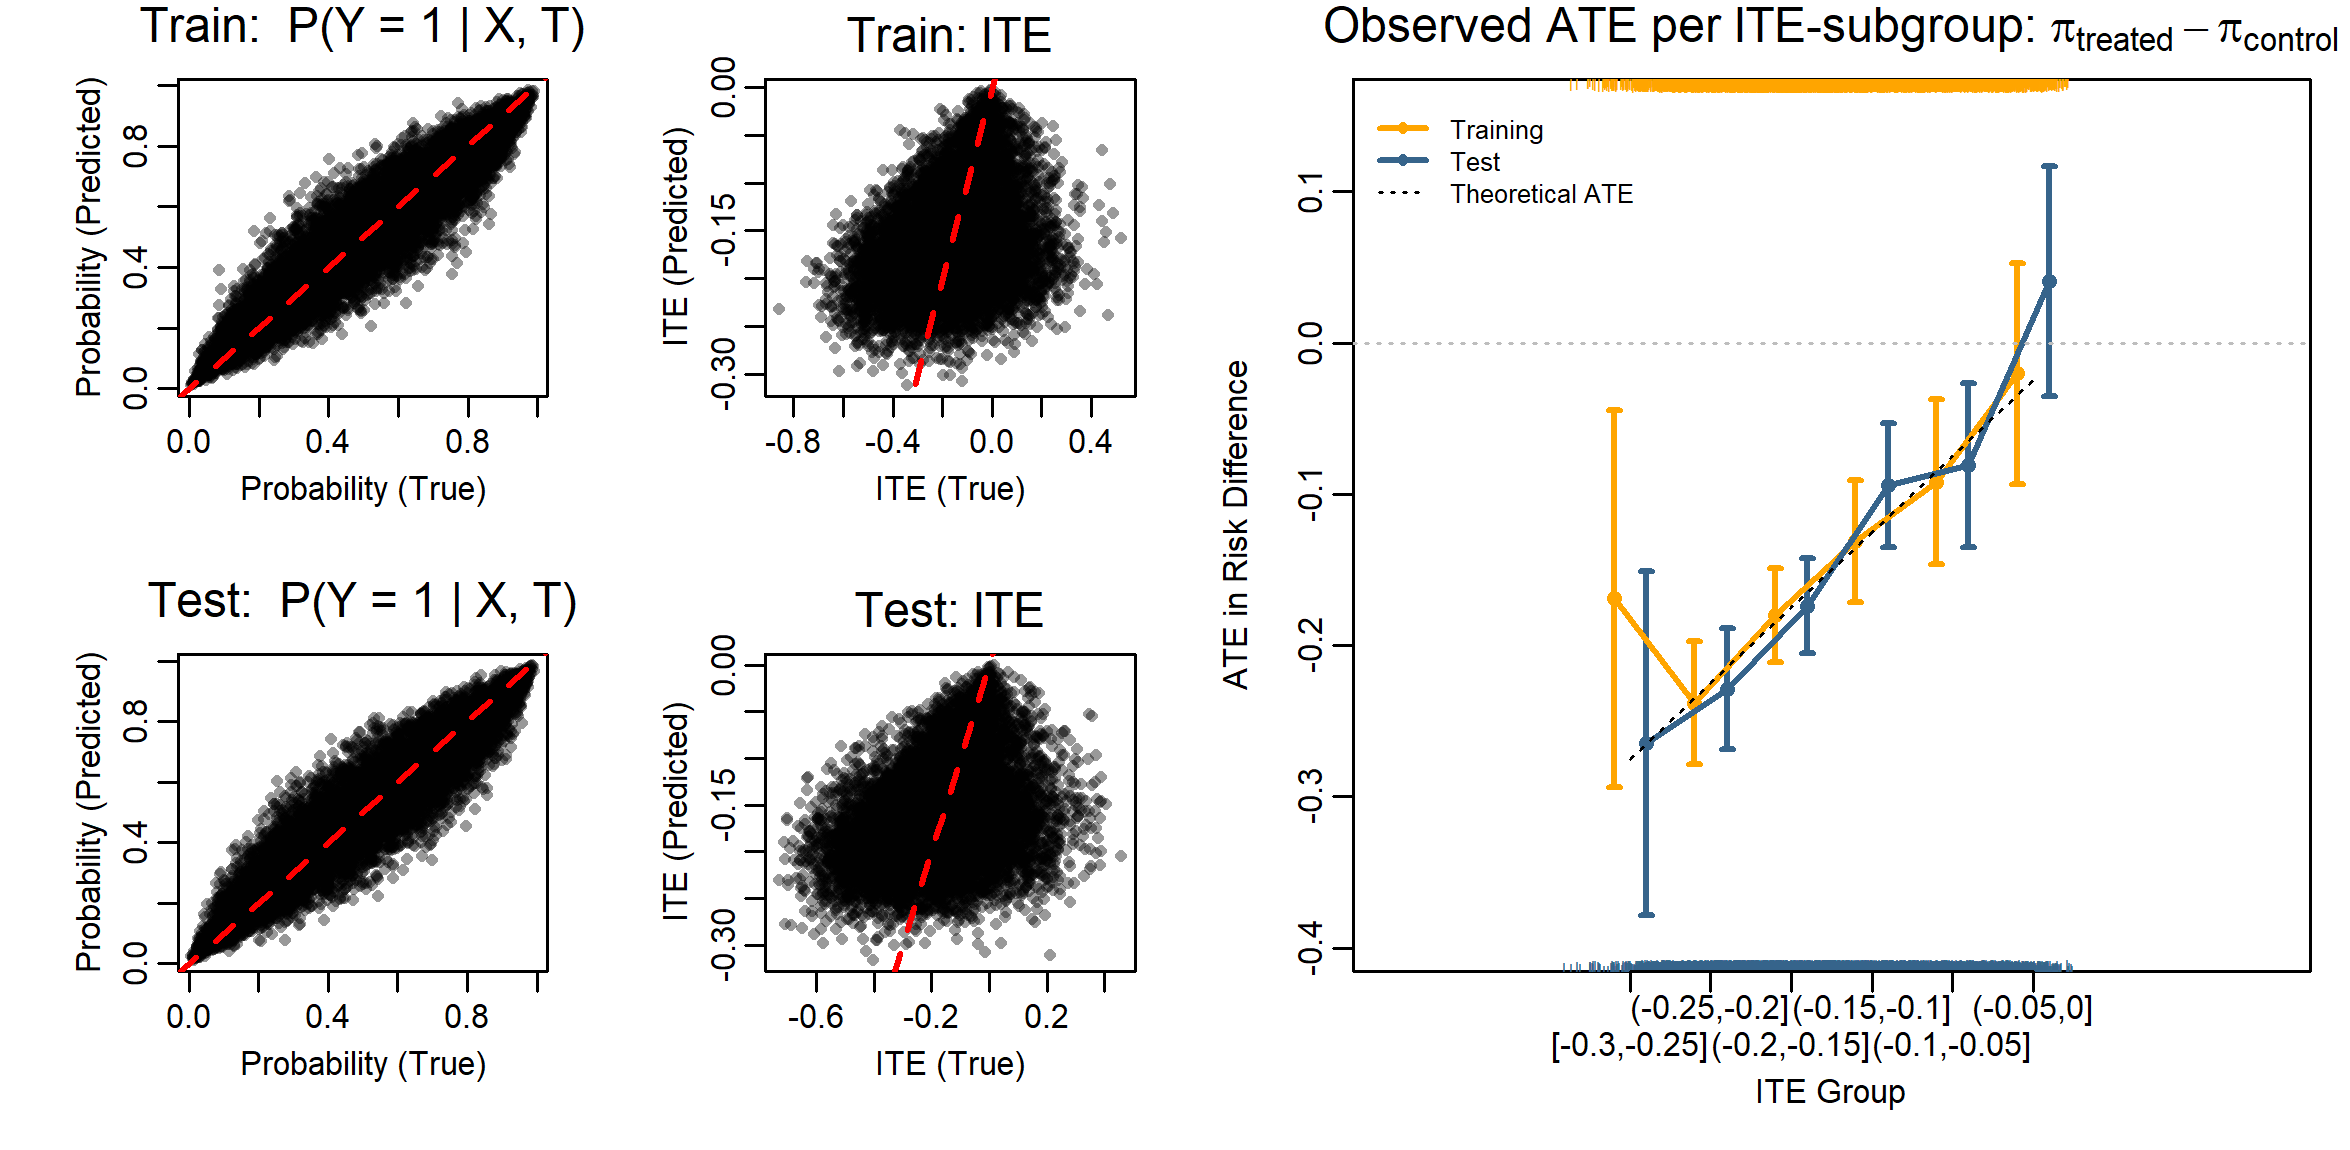
\includegraphics[width=0.9\textwidth]{img/results_ITE_simulation/unobserved_interaction_glm_tlearner.png}
\caption{Results of the T-learner logistic regression in Scenario~(2), where there are strong treatment and interaction effects, but variable $X_1$ is not observed. Left: true vs. predicted probabilities for $\text{P}(Y = 1 \mid X, T)$; Middle: true vs. predicted ITEs; Right: observed ATE in terms of risk difference per estimated ITE subgroup.}
\label{fig:unobserved_interaction_glm_tlearner}
\end{figure}



\begin{figure}[htbp]
\centering
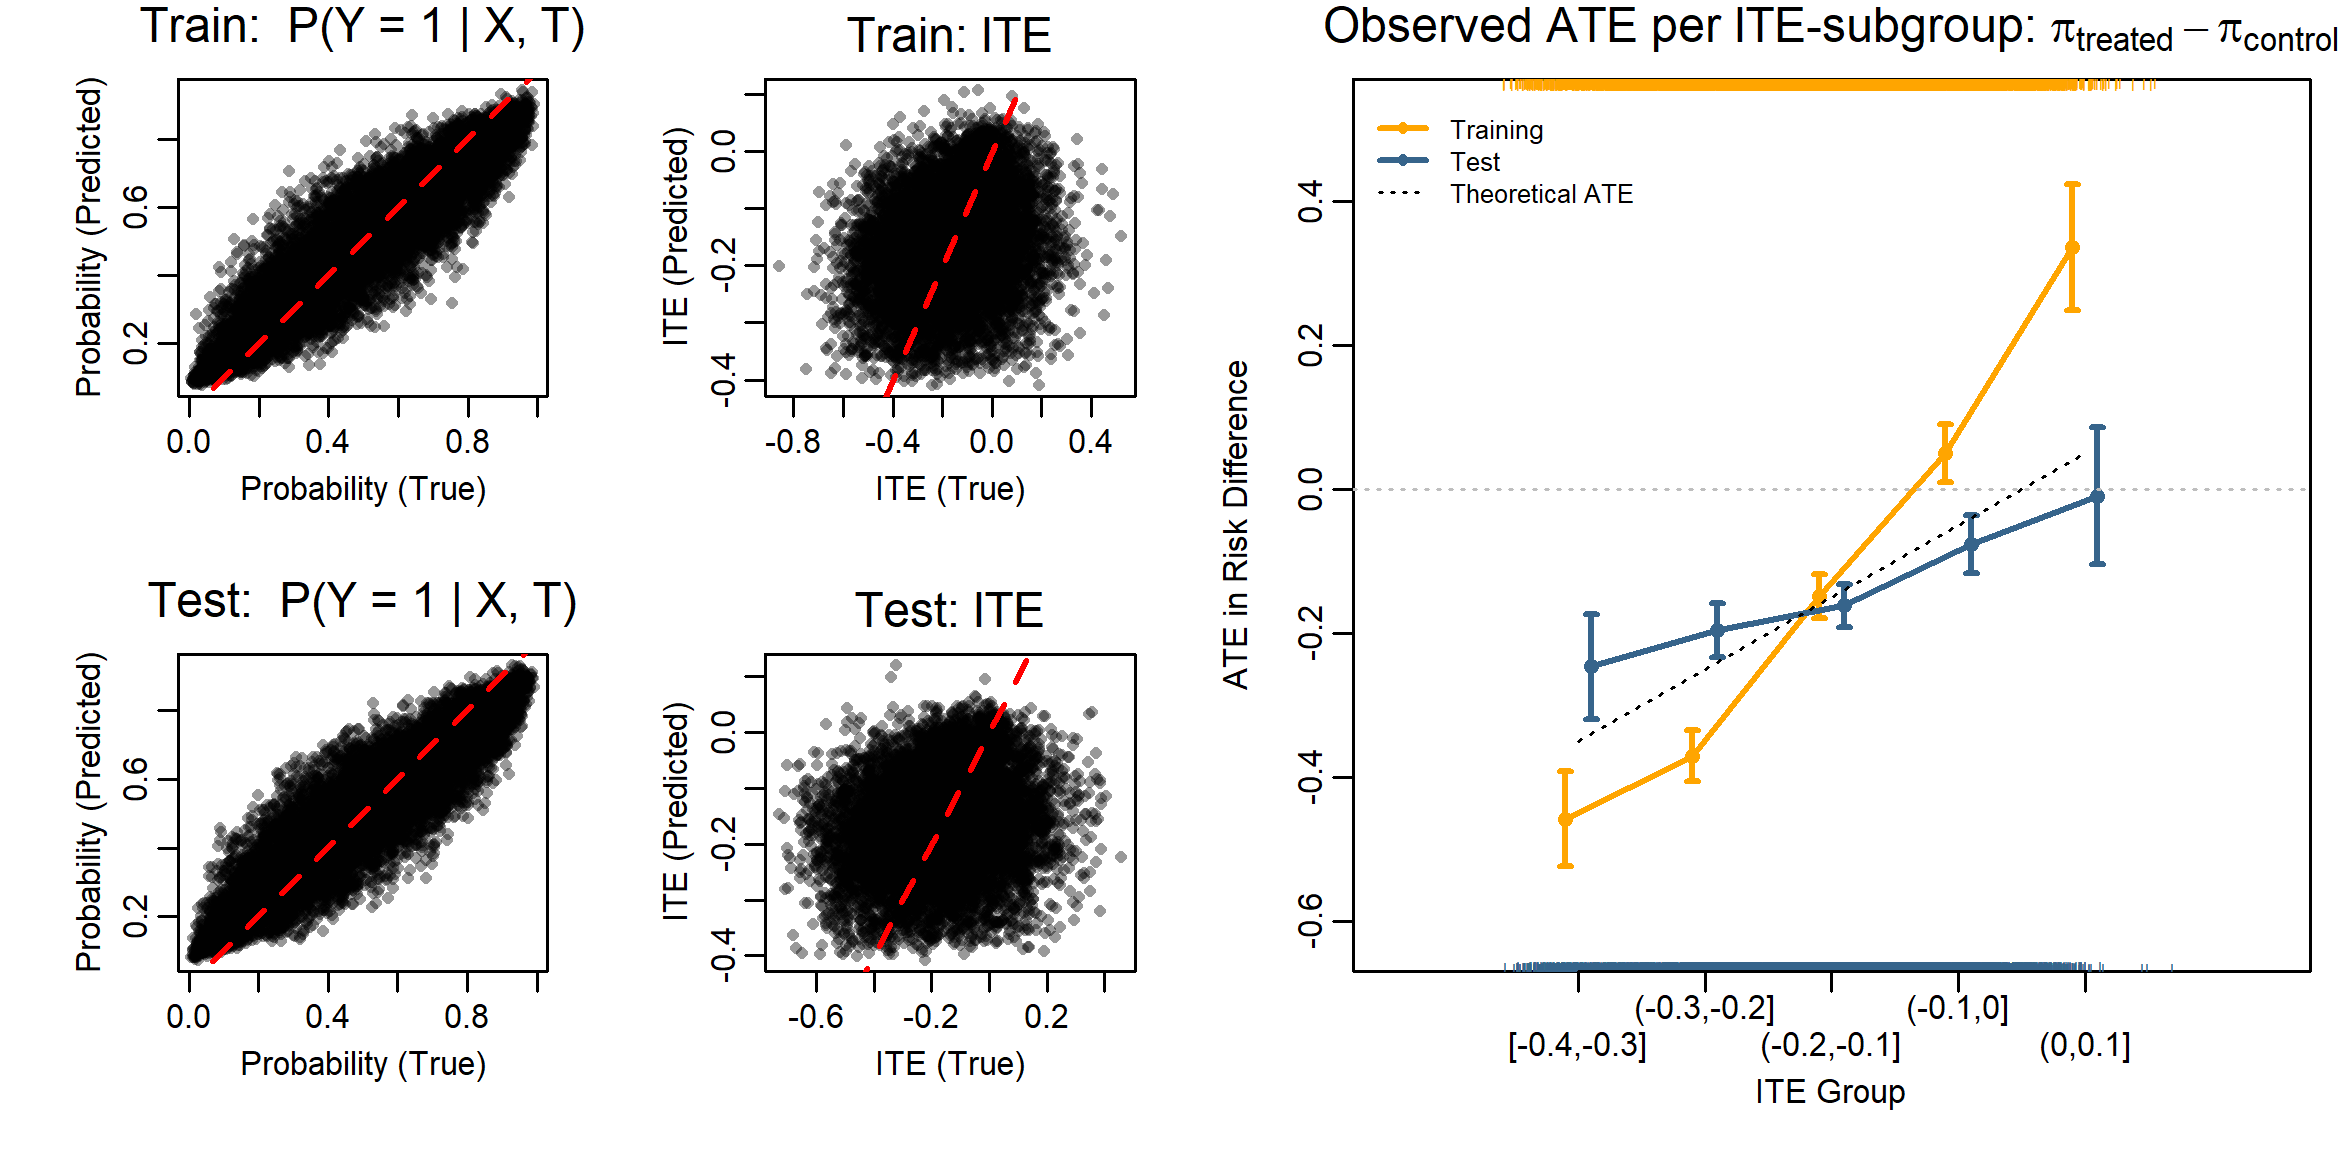
\includegraphics[width=0.9\textwidth]{img/results_ITE_simulation/unobserved_interaction_tuned_rf_tlearner.png}
\caption{Results of the T-learner tuned random forest in Scenario~(2), where there are strong treatment and interaction effects, but variable $X_1$ is not observed. Left: true vs. predicted probabilities for $\text{P}(Y = 1 \mid X, T)$; Middle: true vs. predicted ITEs; Right: observed ATE in terms of risk difference per estimated ITE subgroup.}
\label{fig:unobserved_interaction_tuned_rf_tlearner}
\end{figure}


\clearpage

\subsection{Scenario (3): Fully observed, small effects}

\begin{figure}[htbp]
\centering
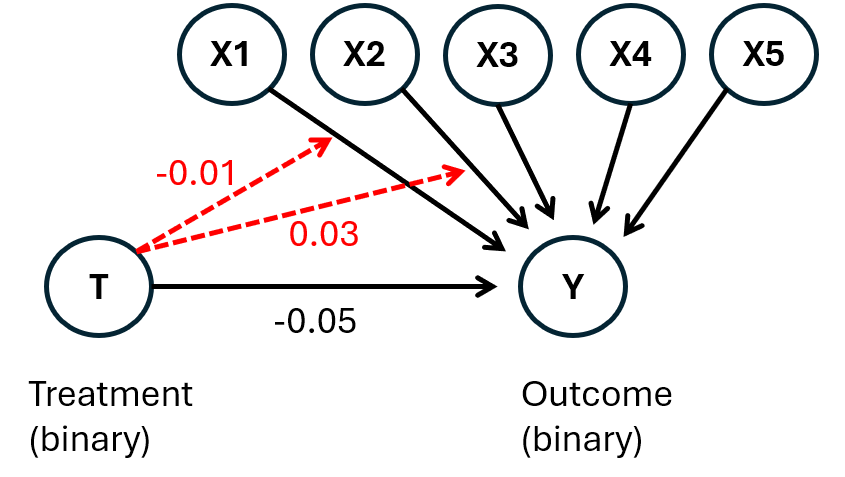
\includegraphics[width=0.35\textwidth]{img/results_ITE_simulation/simulation_small_effects.png}
\caption{DAG for Scenario~(3), where all variables are observed and both treatment and interaction effects are weak. This DAG was previously shown in Figure~\ref{fig:simulation_dags} and is re-plotted here for convenience. The numbers indicate the coefficients on the log-odds scale. Red arrows represent interaction effects between treatment ($T$) and covariates ($X_1$ and $X_2$) on the outcome ($Y$).}
\label{fig:small_interaction_dag}
\end{figure}




\begin{figure}[htbp]
\centering
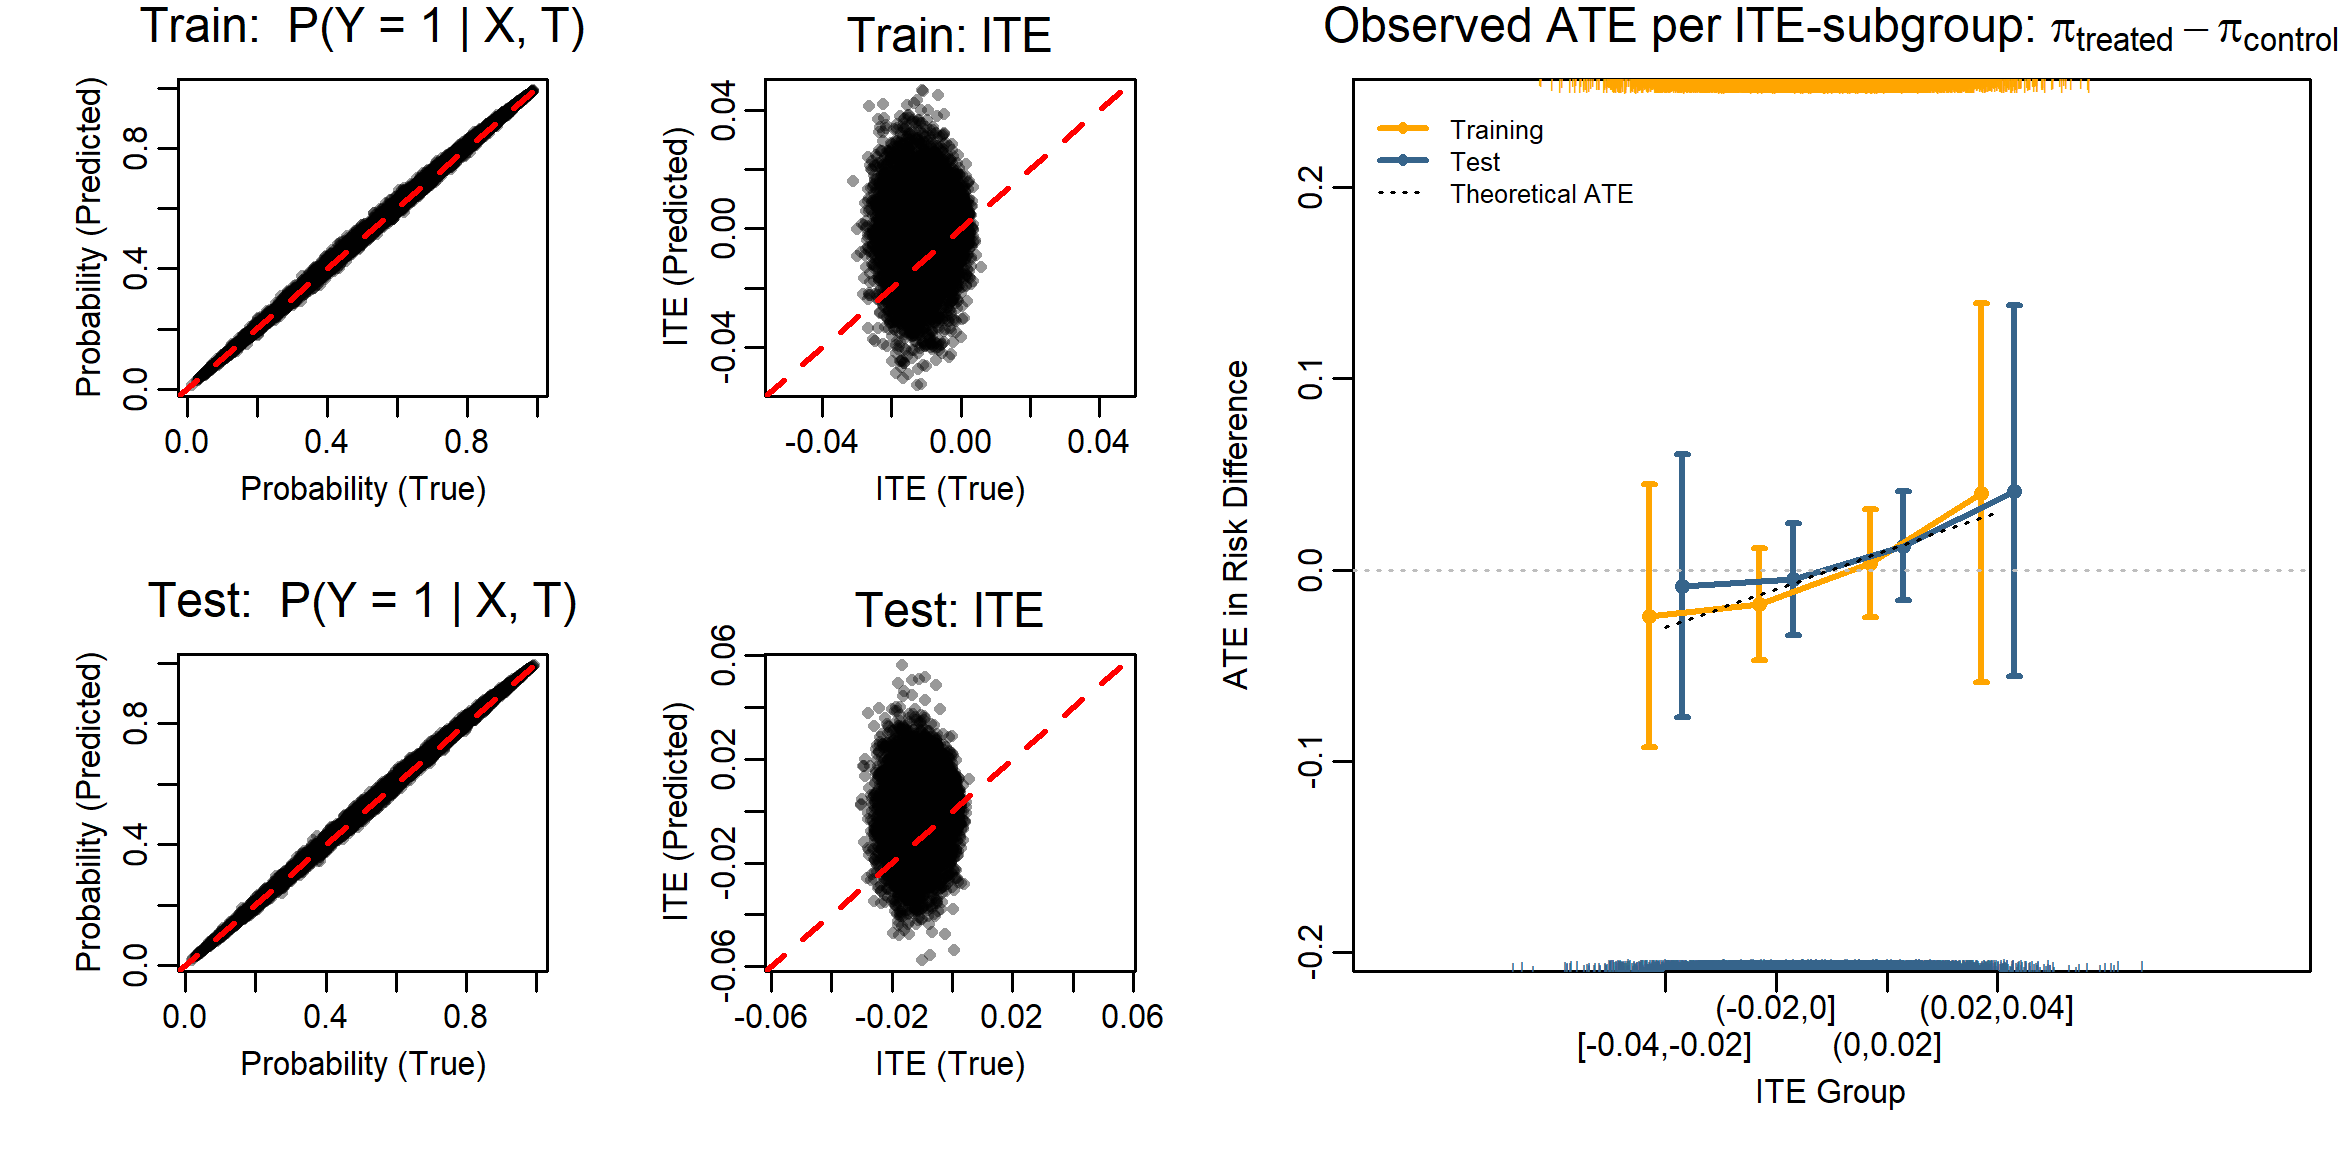
\includegraphics[width=0.9\textwidth]{img/results_ITE_simulation/small_interaction_glm_tlearner.png}
\caption{Results of the T-learner logistic regression in Scenario~(3), where the DAG is fully observed and both treatment and interaction effects are weak. Left: true vs. predicted probabilities for $\text{P}(Y = 1 \mid X, T)$; Middle: true vs. predicted ITEs; Right: observed ATE in terms of risk difference per estimated ITE subgroup.}
\label{fig:small_interaction_glm_tlearner}
\end{figure}




\begin{figure}[htbp]
\centering
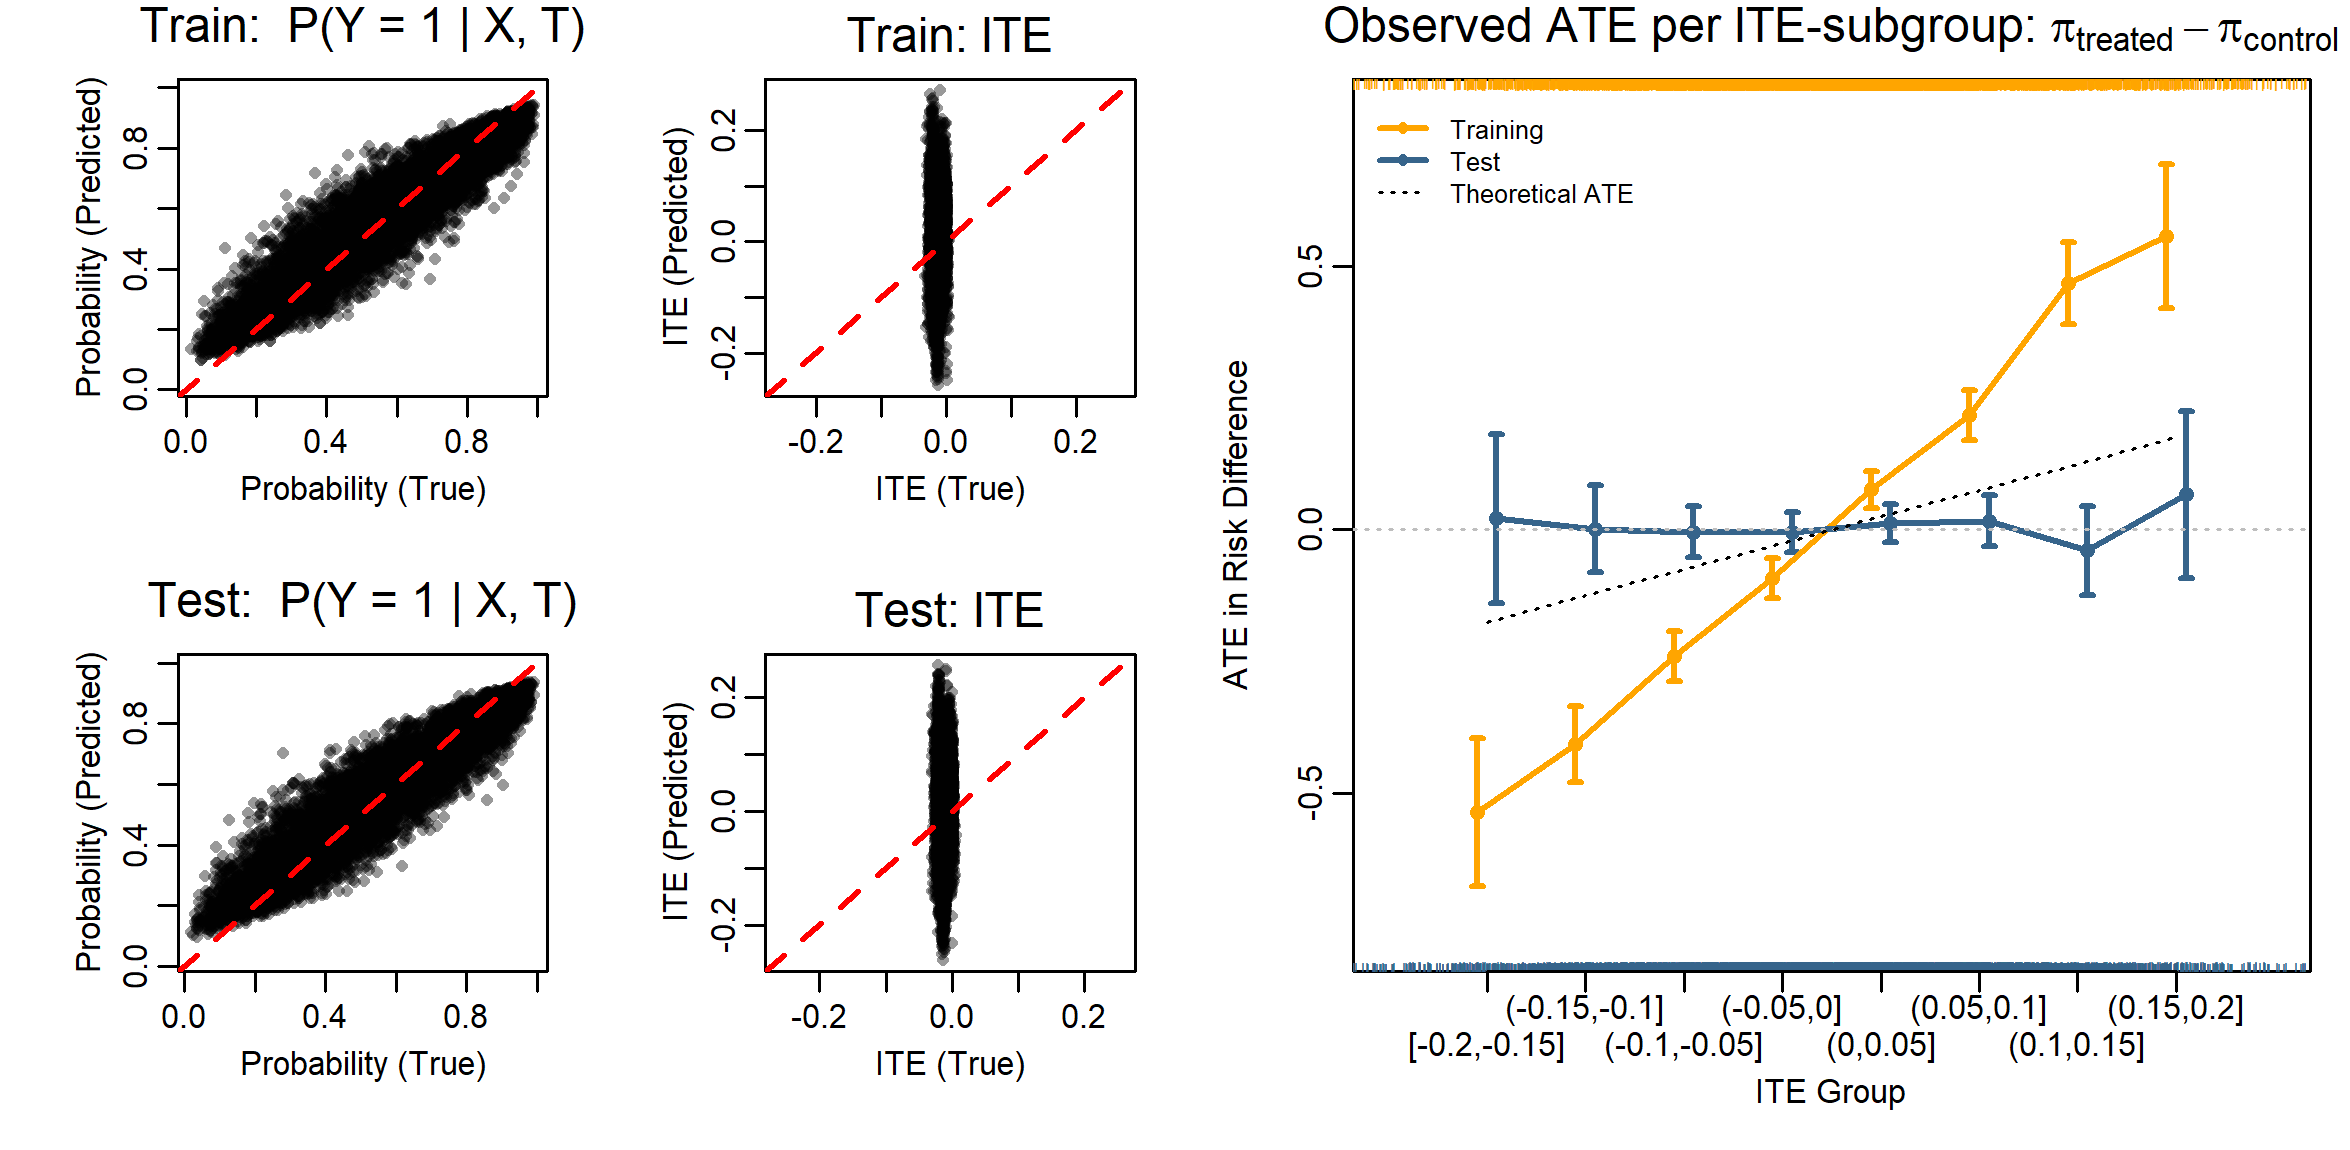
\includegraphics[width=0.9\textwidth]{img/results_ITE_simulation/small_interaction_tuned_rf_tlearner.png}
\caption{Results of the T-learner tuned random forest in Scenario~(3), where the DAG is fully observed and both treatment and interaction effects are weak. Left: true vs. predicted probabilities for $\text{P}(Y = 1 \mid X, T)$; Middle: true vs. predicted ITEs; Right: observed ATE in terms of risk difference per estimated ITE subgroup.}
\label{fig:small_interaction_tuned_rf_tlearner}
\end{figure}


% enforce that starts after all floats have been displayed
\FloatBarrier




\section{Discussion} \label{sec:disc_experiment3}



In Scenario~1, where treatment effect heterogeneity was large and all covariates were observed, the T-learner logistic regression accurately estimated the ITE. The observed ATE, conditional on the respective ITE subgroup, was well calibrated in both the training and test datasets, as shown in the ITE-ATE plot in Figure~\ref{fig:fully_observed_glm_tlearner}. This is as expected, since the data were generated with the same model class (logistic regression), and applying logistic regression as a T-learner for ITE estimation can accurately capture the interaction effects.

The tuned random forest model also performed well. As illustrated in Figure~\ref{fig:fully_tuned_rf_tlearner}, choosing a different model class than that used in the DGP may lead to worse prediction accuracy in terms of $\text{P}(Y = 1 \mid X, T)$ and ITE. This difference between the two models arises because the logistic regression model has only a small number of parameters, and with sufficient data, these parameters can converge to their true values as used in the logistic DGP, allowing near-perfect recovery of the true probabilities and thus ITEs. In contrast, the non-parametric random forest must infer the underlying probabilities from the observed binary outcomes (0 or 1), which are themselves realizations of a Bernoulli process. This introduces inherent noise, making it harder for the model to estimate the true risk accurately -- even with large sample sizes. Nonetheless, the tuned random forest also captured the general trend of the ITEs, as reflected in the ITE-ATE plot, Figure~\ref{fig:fully_tuned_rf_tlearner}. Both models were able to capture treatment effect heterogeneity well under full observability of covariates.



In contrast, the default random forest (i.e., without hyperparameter tuning) performed worse than its tuned counterpart (see Appendix~\ref{sec:default_rf_ite}). As shown in the corresponding ITE-ATE plot, Figure~\ref{fig:fully_observed_rf}, the model exhibited poor calibration and inaccurate ITE estimates, highlighting the importance of proper tuning to ensure reliable ITE estimation and avoid overfitting.


\medskip


\medskip


In Scenario~2, where treatment effect heterogeneity remained large but one important interaction covariate ($X_1$) was not observed, prediction accuracy decreased for both models, and the estimated heterogeneity in terms of the ITE was smaller than the true heterogeneity. Although not all heterogeneity could be recovered, the T-learner logistic regression still estimated the ITEs in the correct direction. As shown in Figure~\ref{fig:unobserved_interaction_glm_tlearner}, the confidence intervals for the ATE per ITE subgroup covered the calibration line. This indicates that individuals estimated to have a smaller ITE indeed experienced worse outcomes under treatment compared to untreated individuals in the same subgroup. Although a considerable number of individuals had a true ITE that was positive, the T-learner logistic regression did not predict a single positive ITE. This shows that the missing covariate $X_1$ prevents detection of individuals who would actually benefit from the treatment. 

In contrast, the T-learner tuned random forest estimated larger treatment effect heterogeneity than the logistic model, but still could not accurately estimate the ITE and also failed to detect patients who would benefit from the treatment. The ITE-ATE plot in Figure~\ref{fig:unobserved_interaction_tuned_rf_tlearner} illustrates that the model discriminates too strongly in the training set and does not generalize well to the test set.


% This is likely due to the fact that the tuned random forest model is a non-parametric model that tries to fit the data as closely as possible, which can lead to overfitting when crucial variables are missing.
\medskip


In Scenario~3, where the true treatment effect heterogeneity was small and all covariates were observed, the T-learner logistic regression estimated a larger heterogeneity than actually present. In the ITE-ATE plot in Figure~\ref{fig:small_interaction_glm_tlearner}, the confidence intervals of all ITE subgroups overlap and include the zero line, indicating that the treatment effect is not significantly different from zero. This matches expectations given the small true effect sizes.

However, the T-learner tuned random forest model incorrectly estimated even larger treatment effect heterogeneity than the logistic regression model. As shown in Figure~\ref{fig:small_interaction_tuned_rf_tlearner}, the model exhibited strong discrimination in the training set but did not to replicate this pattern in the test set, where -- regardless of the estimated ITE -- the observed outcomes in the subgroups were similar.


\medskip


Tuning more flexible models like random forests using cross-validation improved generalization to the test set but led to poor calibration in terms of predicted probabilities vs. empirically observed outcomes in the training set. An illustrative case is shown in Appendix~\ref{sec:calibration_tuned_rf} for the T-learner tuned random forest in Scenario~3 (with weak effects), where calibration was poor in the training set but aligned well with the identity line in the test set. We repeatedly observed this pattern in the tuned random forest when, in the ITE-ATE plot, results from the training set did not generalize to the test set. This highlights the importance of evaluating models on an independent test set, when tuning a model to prevent overfitting. Although, evaluation on a test set should be done in any case.

\medskip

In this experiment, we showed that even when causal ML models for ITE estimation are well calibrated in terms of prediction accuracy $\text{P}(Y = 1 \mid \mathbf{X}, T)$, they can still fail to estimate the ITE accurately under less favorable scenarios. In cases of full observability of covariates but low interaction effects, models may estimate too high heterogeneity that is not present in the data. However, this can become visible in the ITE-ATE plot on the test set, which reveals that the apparent heterogeneity does not generalize. 
But we also observed that when important effect-modifying covariates are missing, the models may fail to detect treatment effect heterogeneity altogether, as shown in Scenario~2. In such cases, the estimated ITEs may be too small or even negative, suggesting that the model does not capture the true treatment effect heterogeneity. This makes it difficult to distinguish between a true lack of heterogeneity and the failure to capture it due to unobserved effect modifiers.


\citet{vegetabile2021} also analyzed the effect of unobserved interaction variables. He pointed out that as long as all confounding variables $\mathbf{X}$ are observed and conditioned on, the ignorability assumption required for ITE estimation is satisfied -- even in the presence of an unobserved interaction variable $Z$. However, if such a variable $Z$ exists, the estimated ITEs would be biased, and this issue could arise even in an RCT setting where confounding is removed through randomization.

\citet{nichols2007} discusses various methods for estimating causal effects from observational data, including in the presence of unobserved variables. One of these methods, instrumental variables (IV), can help reduce bias from unobserved confounding. Whether IV methods can also address unobserved effect modifiers in the context of ITE estimation is not something we explored, and remains beyond the scope of this thesis.



% such as the use of instrumental variables (IV) to estimate CATE in the presence of unobserved confounders \citep{nichols2007, hartford2017}. \citet{frauen2023} propose a model based on IV that is said to also be applicable on observational data. However, this is not yet widely adopted and remains an area for future research.

 % check more details, they also have an example DAG, however it is not yet accepted and still under review








%%%%%%%%%%%%%%%%%%%%%%%%%%%%%%%%%%%%%%%%%%%%%%%%%%%%%%%%%%%%%%%%%%%%%%
%%%%%%%%%%%%%%%%%%%%%%%%%%%%%%%%%%%%%%%%%%%%%%%%%%%%%%%%%%%%%%%%%%%%%%

% 

% LaTeX file for Chapter Exp4
















\chapter{Experiment 4: ITE estimation with TRAM-DAGs (simulation)}




% quantile treatment effect
% Papers:

% https://journals.sagepub.com/doi/pdf/10.1177/1536867X1001000309
% https://epge.fgv.br/files/1125.pdf



\section{Motivation}

We claim that the TRAM-DAG framework can be effectively used for ITE estimation on observational data with confounding and mediating variables, provided that the identifiability assumptions are satisfied and the DAG is fully known. Therefore, we apply TRAM-DAGs in both a confounded and a randomized setting, using data simulated according to the DAGs shown in Figure~\ref{fig:ite_dag_observational}. The binary treatment ($X_4$) is the intervention variable, and the goal is to estimate the ITE for the continuous outcome $Y$.


\begin{figure}[H]
\centering
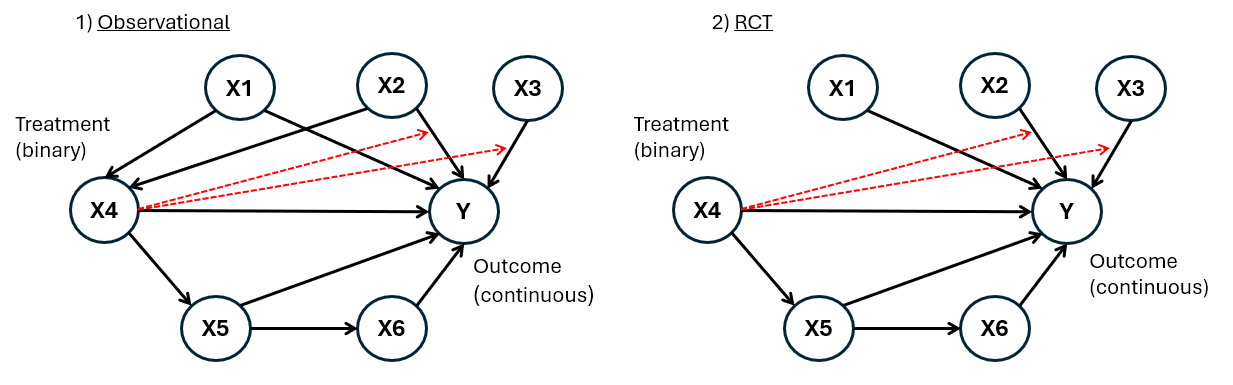
\includegraphics[width=0.85\textwidth]{img/exp4_dags.png}
\caption{DAGs used for the simulation to estimate the ITE. Left: observational; Right: RCT setting. The source nodes $X_1$, $X_2$, and $X_3$ come from a multivariate standard normal distribution ($\rho=0.1$). In the observational setting, the binary treatment $X_4$ depends on the parents $X_1$ and $X_2$. In the RCT setting, this dependency is omitted due to randomization. The outcome $Y$ depends on all variables, with additional interaction effects between the treatment and the variables $X_2$ and $X_3$. All variables except the treatment $X_4$ are continuous.}
\label{fig:ite_dag_observational}
\end{figure}

\medskip

\textbf{Illustrative scenario:} An possible real-world scenario that follows the structure of the proposed DAG could be the following: A marketing campaign is conducted to increase customer spending. The treatment is the marketing email ($X_4$) sent to customers. If the treatment is not randomized, it depends on prior total spend ($X_1$) and the customer engagement score ($X_2$). The outcome is the total spend in the 30 days following the email, denoted as $Y$. The past total spend ($X_1$) and customer engagement score ($X_2$) act as confounders, influencing both the treatment and the outcome. The customer satisfaction score ($X_3$), obtained from a recent survey, is another predictor. The time spent on the website after receiving the email ($X_5$) is a mediator that affects the number of product pages viewed ($X_6$), which in turn influences the total spend ($Y$). Interaction effects exist between the treatment ($X_4$) and both $X_2$ and $X_3$, meaning the treatment effect differs based on the customer's engagement and satisfaction levels. The goal is to estimate the individualized treatment effect (ITE) of the marketing email ($X_4$) on the total spend ($Y$), in order to personalize customer targeting.

\medskip

\section{Setup} \label{sec:methods_experiment4}

\textbf{Data-generating process:} The standard logistic distribution was chosen as the noise distribution to align with other examples in this thesis. Any other noise distribution could also be used here, as we are not interested in coefficient interpretability in this experiment. All variables except the binary treatment $X_4$ are continuous. The source nodes $X_1$, $X_2$, and $X_3$ are generated from a multivariate standard normal distribution with a compound symmetric covariance matrix ($\rho = 0.1$). These variables represent baseline patient characteristics.

In the observational setting, $X_1$ and $X_2$ act as confounders by influencing both the treatment assignment $X_4$ and the outcome $Y$. In the RCT setting, these dependencies are removed due to randomization. The mediator $X_5$ depends on treatment $X_4$, and $X_6$ depends on $X_5$. The log-odds of the continuous outcome $Y$ depend linearly on all covariates, including additional interaction terms between the treatment and $X_2$ and $X_3$. Equation~\ref{eq:outcome_dgp} defines the outcome on the log-odds scale:

\begin{equation}
h(y \mid \mathbf{X}) = h_I(y) + \boldsymbol{\beta}_X^\top \mathbf{X} + X_4 \cdot (\boldsymbol{\beta}_{TX}^\top \mathbf{X}_{\text{TX}})
\label{eq:outcome_dgp}
\end{equation}

Here, $h_I(y)$ is the intercept function, $\mathbf{X}$ is the full covariate vector, and $\mathbf{X}_{\text{TX}} = \{X_2, X_3\}$ denotes the interaction covariates that affect the outcome only when treatment is applied ($X_4 = 1$). The intercept function $h_I(y)$ must be smooth and monotonically increasing. We define it as $h_I(y) = \tan(y/2) / 0.2$ for $y \in [-2, 2]$, and extrapolate linearly at the boundaries.

The coefficients are set as $\boldsymbol{\beta}_X = (-0.5,\ 0.5,\ 0.2,\ 1.5,\ -0.6,\ 0.4)$, where the value $1.5$ represents the direct effect of treatment $X_4$ on the outcome. The interaction coefficients are set to $\boldsymbol{\beta}_{TX} = (-0.9,\ 0.7)$.

\medskip

\textbf{Three scenarios:} The experiment is conducted under three different scenarios regarding the effect of the treatment on the outcome $Y$ in the DGP: (1) both direct and interaction effects, (2) only a direct effect, and (3) only interaction effects. Depending on the scenario, the corresponding coefficients in $\boldsymbol{\beta}_X$ and $\boldsymbol{\beta}_{TX}$ are set to zero.

\medskip


\textbf{TRAM-DAG estimation:} In both the observational and RCT settings, the TRAM-DAG is fitted as an S-learner (i.e., a single model including the treatment variable). To allow for full flexibility, all nodes with parents are modeled using complex intercepts with three hidden layers of size (10, 10, 10), without batch normalization or dropout, unsing ReLU activation. This architecture enables the model to learn nonlinearities and interactions between the treatment and covariates, allowing it to estimate both potential outcomes. The model is trained on a dataset of 20,000 samples. To prevent overfitting, an additional validation set of 10,000 samples is used, and the final model is selected using early stopping based on validation loss.

\medskip

\textbf{ITE estimation procedure:} In contrast to most of the research we analyzed, where ITEs are typically defined in terms of expected values of potential outcomes, we estimate the quantile treatment effect (QTE), specifically at the median. For each individual, we calculate the difference between the medians of the potential outcome distributions under treatment and control. \citet{chernozhukov2005}, for example, highlighted the ability of quantile regression models in heterogeneous treatment effect estimation. QTEs are particularly relevant when the distributional behavior of outcomes beyond the mean is of interest. The median QTE is defined as

\begin{equation}
\text{QTE}^{(0.5)}(\mathbf{x}) = Q_{Y(1) \mid \mathbf{X} = \mathbf{x}}(0.5) - Q_{Y(0) \mid \mathbf{X} = \mathbf{x}}(0.5),
\label{eq:qte}
\end{equation}


where $Q_{Y(t) \mid \mathbf{X} = \mathbf{x}}(q)$ denotes the $q$-th quantile of the potential outcome distribution under treatment $t$.

Once the TRAM-DAG model is fitted on observed data, we can access the inverse transformation functions $X_i = h^{-1}(Z_i \mid \text{pa}(X_i))$, which represent the structural equations of the DAG. ITE estimation proceeds in three steps, according to Algorithm~\ref{alg:ite_qte}. First, the latent values $z_{ij}$ for the explanatory variables $X_i \in \{X_1, X_2, X_3, X_5, X_6\}$ are computed for each sample $j$ using the transformation functions conditioned on their observed parents. Second, the treatment variable $X_4$ is intervened on using the do-operator for both $X_4 = 0$ and $X_4 = 1$. For each of these two treatment states, $X_5$, $X_6$, and the potential outcome (distribution) $Y$ are sampled sequentially using the latent encodings and inverse transformations. This means that the counterfactuals for $X_5$ and $X_6$ are determined. This results in two potential outcome distributions per individual, as illustrated in Figure~\ref{fig:exp4_potential_outcomes}. Finally, for each individual, the median is determined for both potential outcome distributions and the QTE is calculated as the difference between the two medians. Note that estimating the potential outcomes in terms of expected values would also be possible -- either by repeatedly sampling from each outcome distribution or, potentially, by numerical integration. However, for this experiment, we chose to estimate the QTE. For simplicity, we will refer to these as ITEs throughout the remainder of the experiment.


\begin{figure}[H]
\centering
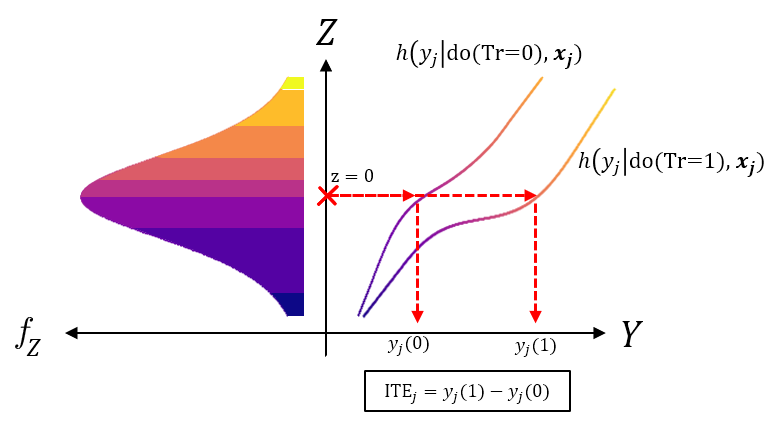
\includegraphics[width=0.6\textwidth]{img/potential_outcomes_y.png}
\caption{ITE estimation in terms of quantile treatment effect (QTE) at the median with TRAM-DAGs. The two transformation functions represent the distributions of the potential outcomes under both treatments. For the QTE(0.5), the median of the latent distribution (0 for the standard logistic) is evaluated on both transformation functions to determine the median potential outcomes. We define the ITE for an individual as the difference of the median potential outcomes.}
\label{fig:exp4_potential_outcomes}
\end{figure}


\begin{algorithm}
\caption{ITE estimation (QTE) using TRAM-DAGs}
\label{alg:ite_qte}
\begin{algorithmic}
\State \textbf{Input:} Fitted TRAM-DAG, dataset of $n$ individuals
\For{each individual $j = 1$ to $n$}
  \State \textbf{Step 1: Determine latent values}
  \For{each explanatory node $X_i \in \{X_1, X_2, X_3, X_5, X_6\}$}
    \State Compute latent value: $z_{ij} = h_i(x_{ij} \mid \text{pa}(x_{ij}))$
  \EndFor

  \State \textbf{Step 2: Generate potential outcomes under treatment and control}
  \For{$x_4 \in \{0, 1\}$} \Comment{Simulate both treatment states}
    \State Fix $X_4 = x_4$ (intervention)
    \State Sample $X_5$ and $X_6$ sequentially using $z_{ij}$ and inverse transformations
    \State Sample potential outcome $y_j(x_4)$ using $z_{7,j} = 0$ (median of the potential outcome distribution)

  \EndFor

  \State \textbf{Step 3: Compute ITE (QTE) for individual $j$}
  \State $\text{ITE}_j = y_j(1) - y_j(0)$  %\text{median}(y_j(1)) - \text{median}(y_j(0))$
\EndFor
\State \textbf{Output:} ITE estimates $\{\text{ITE}_j\}_{j=1}^n$
\end{algorithmic}
\end{algorithm}


\medskip

\textbf{Model evaluation:} Validation is conducted on the training dataset and on an independent test dataset of same size. During the data-generating process, the true potential outcomes under both treatment states were recorded for each individual, which allows for exact computation of the true ITE. The estimated ITEs are evaluated against the true values using several visual and numerical metrics. These include density plots of the estimated ITEs, scatter plots of true vs. estimated ITEs, and ITE-ATE plots where the observed ATE per ITE subgroup is computed as the difference in medians. In addition, the average of the estimated ITEs is compared to the true average ITE and to the empirical ATE from the RCT setting. The scatter plot of true versus estimated ITEs is the most informative validation, as it directly reflects how accurately the model estimated ITEs.














% 
% \textbf{ITE estimation procedure: } In contrast to the potential outcomes framework, where the potential outcomes are defined as the expected value of the outcome under treatment, we define the potential outcomes as the median of the outcome distribution under treatment - the quantile treatment effect (QTE). For simplicity, we will further refer to the individual treatment effect as ITE even though technically, the QTE is meant. Determining the potential outcomes in terms of the expected values would also be possible, but would require us to repeatedly sample from each resulting potential outcome distribution for each individual and average the results. This was computationally too time consuming and therefore we decided to estimate the QTE instead. In the ITE estimation in the previous examples with binary outcome, this was not necessary, since the potential outcomes were defined as the probabilities of the outcome under treatment and control, hence a single number that represents the expected value.
% 
% Notes after Meeting 24.06.25: Depending on the problem, CATE in terms of expected values of potential outcomes might be more appropriate than QTE, but also QTE could be better. Depends. If we wanted the potential outcomes based on the expected values, we have two options. either sample latent values and evaluate inverse tranformation functions. from those two sample distributions calculate the means to get the expected potential outcomes. Lucas suggested that we could also use numerical integreation instead, then we would not have to sample.
% 
% In contrast to the mean-based estimands above, the quantile treatment effect (QTE) evaluates differences in the distribution of potential outcomes. For instance, the median treatment effect is defined as
% 
% \citep{chernozhukov2005} also wrote about QTE (also in the context of instrumental variables). (also says to can deal with unobserved heterogeneity.. although, probably only as extension of our approach)
% 
% \begin{equation}
% \tau^{(0.5)}(x) = Q_{Y(1) \mid X = x}(0.5) - Q_{Y(0) \mid X = x}(0.5),
% \end{equation}
% 
% where $Q_{Y(t) \mid X = x}(q)$ denotes the $q$-th quantile of the potential outcome under treatment $t$. QTEs are particularly relevant when treatment effects are not symmetrically distributed or when tail behavior is of interest. In experiment 4, Section \ref{sec:methods_experiment4} we performed a simulation study using the median for the QTE estimation.
% 
% Once the TRAM-DAG is fitted, we obtained the estimated (inverse) transformation functions $X_i = h^{-1}(Z_i \mid pa(X_i))$ that represent the equations $X_i = f(Z_i, pa(X_i))$ in the structural causal model. The process for the ITE estimation is outlined in \ref{alg:ite_qte}. It is done as follows: In a first step to estimate the ITE, we determine the latent values $z_{ij}$ in all observed samples $j$ for the explanatory nodes $i$ - X1, X2, X3, X5 and X6. The latent values are the values of the transformation functions at the observed value of the variable given the observed values of its parents $z_{ij} = h_i(x_{ij} \mid pa(x_{ij}))$. In a second step, these latent values $z_{ij}$ are used to sequentially sample from the two interventional distributions when setting the treatment X4 to either 0 or 1. For each individual, these interventions impact the mediator nodes X5 and X6 as well as the outcome Y. The source nodes X1, X2 and X3 remain equal under both treatments. The treatment X4 is the variable which we fix by the do-intervention. X5 and X6 will change according to the treatment. Finally, for each set of samples $j$ (meaning for each individual) we get two distributions for the outcome, one under treatment and one under control. Then, for each individual, we calculate the iTE as the difference between the medians of the potential outcome distributions under treatment and control, as visualized in Figure~\ref{fig:exp4_potential_outcomes}.
% 
% 
% 
% 
% \begin{figure}[H]
% \centering
% 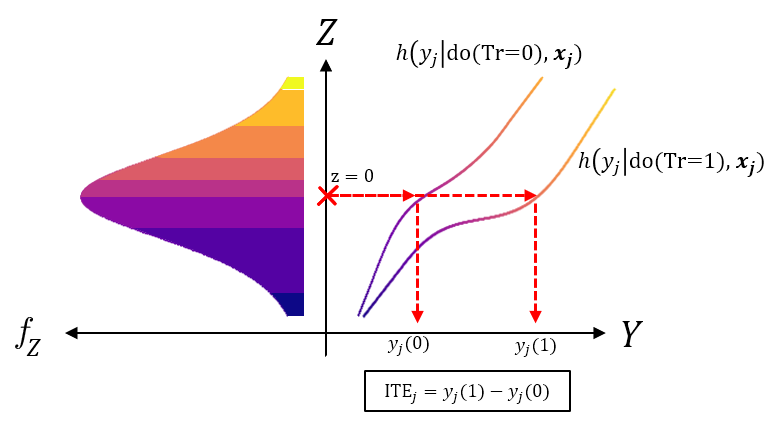
\includegraphics[width=0.6\textwidth]{img/potential_outcomes_y.png}
% \caption{Quantile treatment effect (QTE) at the median with TRAM-DAGs. The two transformation functions represent the distributions of the potential outcomes under both treatmetns. For the QTE(0.5), the median of the latent distribution is evaluated on both transformation functions to determine the median-potential-ouotcomes. This is in contrast to the ITE based on the expected values of the potential outcomes.}
% \label{fig:exp4_potential_outcomes}
% \end{figure}
% 
% 
% 
% 
% \begin{algorithm}
% \caption{ITE Estimation (QTE) Using TRAM-DAG in Observational Data}
% \label{alg:ite_qte}
% \begin{algorithmic}[1]
% \State \textbf{Input:} Fitted TRAM-DAG, observational dataset with $n$ samples
% \For{each sample $j = 1$ to $n$}
%   \State \textbf{Step 1: Encode explanatory nodes}
%   \For{each explanatory node $X_i \in \{X_1, X_2, X_3, X_5, X_6\}$}
%     \State Compute latent value: $z_{ij} = h_i(x_{ij} \mid \text{pa}(x_{ij}))$
%   \EndFor
% 
%   \State \textbf{Step 2: Generate potential outcomes under treatment and control}
%   \For{$x_4 \in \{0, 1\}$} \Comment{Simulate both treatment states}
%     \State Fix $X_4 = x_4$ (intervention)
%     \State Sample $X_5$ and $X_6$ sequentially using $z_{ij}$ and inverse transformations
%     \State Sample potential outcome $y_j^{(x_4)}$ using $z_{7,i} = 0$ (median of the potential outcome distribution)
% 
%   \EndFor
% 
%   \State \textbf{Step 3: Compute QTE for individual $j$}
%   \State $\text{ITE}_j = \text{median}(y_j^{(1)}) - \text{median}(y_j^{(0)})$
% \EndFor
% \State \textbf{Output:} ITE estimates $\{\text{ITE}_j\}_{j=1}^n$
% \end{algorithmic}
% \end{algorithm}
% 
% 
% 
% 
% 
% \textbf{Validation of results: } In the data generating mechanism, along with the actually sampled values, the potential values under both treatments are also recorded and used to determine the true QTE (the ITE based on the 50 percent quantiles of the potential outcome distributions of each individual.)
% The results are displayed by densities of the estimated ITE, the scatterplots of the true vs. estimated ITE, the ITE-ATE plot with the difference in medians as ATE within subgroups to make it comparable to the estimated ITEs. Furthermore the average of all estimated and true (dgp) ITEs are presented in table format. We further calculate the ATE as the overall difference in medians in the RCT setting and compare it to the estimated values based on the ITEs, althogh if this comparison in terms of the mean of a difference in medians is valid we did not further proof. It should be rather regarded as information, but not as proof. The scatterplot of the true vs. estimated ITE poses the most important validation.


% Check if true? probably not entirely... in both, the RCT and in the Observational setting, also other models could be applied instead of TRAM-DAG. As long as all confounders are included in the model, we controll for the confounders and can get unbiased results. For example a T-learner Colr($Y \sim X_1 + X_2 + X_3$) (because Colr is basically what we did in the DGP) fitted on both treatment groups separately could be used to estimate the ITE in our proposed experiment. This might only be possible so easily as long as we do not assume additional interactions between the treatment and the mediators $X_5$ and $X_6$. If we would assume such interactions, we would have to include these in the model as well, which would make it more complex and possibliy requires to fit and apply multiple models. If there are no interactions with the mediators, they can be omitted, since we are interested in the total treatment effects and not in separating the effect (mediation analysis). But again, we can only omit if these variables do not contain additional information about treatment effect heterogeneity. The reasoning is because to estimate the total effect one should not control for mediators. (check if really true!!!)  However, the TRAM-DAG framework is well suited to also deal with mediators and calculate counterfactuals, therefore we think it is a good example to show its capabilities.


% Notes after Meeting 24.06.25: Depending on the problem, CATE in terms of expected values of potential outcomes might be more appropriate than QTE, but also QTE could be better. Depends. If we wanted the potential outcomes based on the expected values, we have two options. either sample latent values and evaluate inverse tranformation functions. from those two sample distributions calculate the means to get the expected potential outcomes. Lucas suggested that we could also use numerical integreation instead, then we would not have to sample.











% \begin{table}
% 
% \caption{Comparison of confidence intervals for the mean differences across scenarios. The first row of each pair corresponds to the confidence interval from the linear model (lm), while the second row corresponds to the bootstrap method.}
% \centering
% \begin{tabular}[t]{lrr}
% \toprule
%   & Lower Bound & Upper Bound\\
% \midrule
% Scenario 1 (lm) & -0.58231 & -0.54359\\
% Scenario 1 (bootstrap) & -0.58210 & -0.54355\\
% Scenario 2 (lm) & -0.59118 & -0.55371\\
% Scenario 2 (bootstrap) & -0.59091 & -0.55405\\
% Scenario 3 (lm) & -0.06784 & -0.02799\\
% \addlinespace
% Scenario 3 (bootstrap) & -0.06784 & -0.02752\\
% \bottomrule
% \end{tabular}
% \end{table}

 


\section{Results}

First, we present the results for Scenario (1), which includes both direct and interaction effects  of treatment. Then, we show the results for Scenario (2), which has a direct effect but no interaction effects, and finally Scenario (3), which includes interaction effects but no direct treatment effect. For each scenario, we compare the results in an observational setting with confounded treatment allocation and in a randomized controlled trial (RCT) setting without confounding. We also compare the average treatment effect (ATE), which can be directly calculated in the RCT setting on observed outcomes, with the ATE derived from the estimated ITEs. All ITEs presented in this experiment are technically quantile treatment effects (QTEs), as defined in Equation~\ref{eq:qte}, based on the medians of the potential outcomes. For simplicity, we will refer to them as ITEs. The aim is to investigate how the TRAM-DAG performs in the presence or absence of direct and interaction effects of the treatment, both in confounded and in randomized settings, for the purpose of ITE estimation.

\subsection{Scenario (1): Direct and interaction effects} 


\begin{figure}[H]
\centering
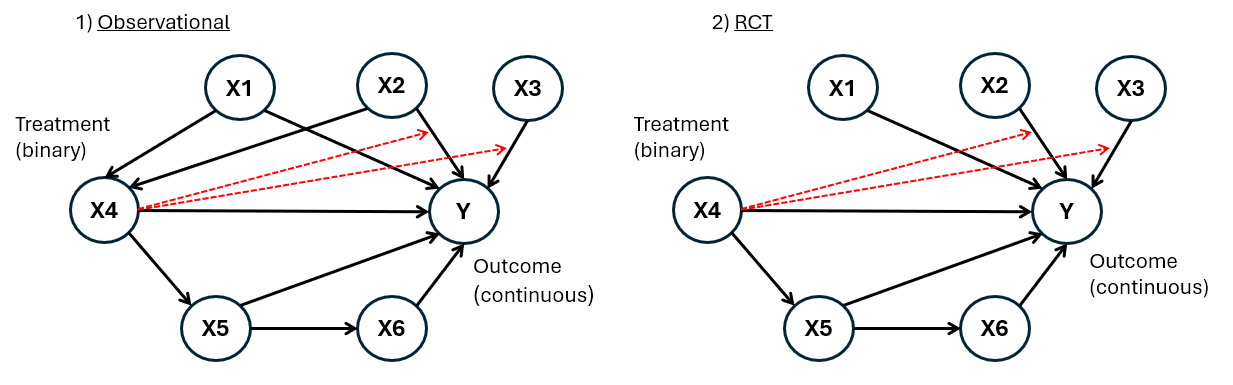
\includegraphics[width=0.85\textwidth]{img/exp4_dags.png}
\caption{DAGs for Scenario~(1), which includes a direct effect of the treatment on the outcome and additional interaction effects with covariates $X_2$ and $X_3$. These DAGs were previously shown in Figure~\ref{fig:ite_dag_observational} and is re-plotted here for convenience. Left: observational setting; Right: RCT setting.}
\label{fig:ite_dag_observational_1}
\end{figure}

Scenario~(1) includes a direct effect of the treatment on the outcome, and interaction effects with $X_2$ and $X_3$, as shown in Figure~\ref{fig:ite_dag_observational_1}. Train and test sets with 20,000 samples each were generated.

In the observational setting, treatment was confounded by $X_1$ and $X_2$. In the train set, $38.6$\% of individuals were in the control group and $61.4$\% in the treatment group. The test set had a similar distribution.

In the RCT setting, treatment was randomly assigned. In the train set, $49.8$\% were in control and $50.2$\% in treatment; in the test set, the shares were $50.2$\% and $49.8$\%, respectively.

Figure~\ref{fig:scenario1_ite_distribution_dgp} shows the true ITE distribution from the DGP, which displays some heterogeneity due to interaction effects. Figure~\ref{fig:scenario1_sampling_distributions_vertical} shows the marginal distributions of all variables in the DGP and as estimated by the TRAM-DAG. The distribution of the outcome $Y$ under $\text{do}(X_4 = 0)$ and $\text{do}(X_4 = 1)$ is shown in Figure~\ref{fig:scenario1_outcome_distributions}. The ITEs were estimated as the difference in medians of the potential outcomes. Figure~\ref{fig:scenario1_ite_densities_train_test} compares the densities of the estimated and true ITEs. In both observational and RCT settings, the estimated ITEs are close to the true ones in both train and test sets. Figure~\ref{fig:scenario1_ite_scatter_train_test} shows the scatterplots of estimated vs. true ITEs. Figures~\ref{fig:observ_scenario1_ite_ATE} and \ref{fig:rct_scenario1_ite_ATE} show the ITE-ATE plots, where the ATE is calculated as the median difference in observed outcomes within ITE subgroups. The trends are similar across train and test sets.



The ATEs calculated based on different measures in both the training and test sets are shown in Table~\ref{tab:scenario1_ate_comparison}. In the RCT setting (training set), the difference in means of the outcomes between the two treatment groups was 
$-0.563$, with a confidence interval of 
$-0.582$ to 
$-0.543$. 



% 
% Scenario (1) included a direct effect of the treatment on the outcome and an additional interaction effect of the treatment with the covariates X2 and X3, as presented in Figure~\ref{fig:ite_dag_observational_1}. A train and test set were generated with 20,000 observations each. 
% In the observational setting, the treatment allocation was confounded by the covariates X1 and X2.  In the train set, $round(observ_scenario1$dev_treatment_allocation[1]*100, 1)$\% of patients were in the control group and $round(observ_scenario1$dev_treatment_allocation[2]*100, 1)$\% were in the treatment group. This ratio was similar in the test set. 
% In the RCT setting treatment allocation was randomized. In the train set $round(rct_scenario1$dev_treatment_allocation[1]*100, 1)$\% individuals were in the control group and $round(rct_scenario1$dev_treatment_allocation[2]*100, 1)$\% in the treatment group. In the test set $round(rct_scenario1$val_treatment_allocation[1]*100, 1)$\% were in the control group and $round(rct_scenario1$val_treatment_allocation[2]*100, 1)$\% in the treatment group. 
% Figure \ref{fig:scenario1_ite_distribution_dgp} illustrates the true ITE distribution that resulted from the DGP. Due to the interaction effects, there is some heterogeneity in the ITE distribution. Figure \ref{fig:scenario1_sampling_distributions_vertical} shows the marginal distributions of all variables according to the DGP and the estimates by the fitted TRAM-DAG. Figure \ref{fig:scenario1_outcome_distributions} shows the distribution of the outcome ($Y$) under the do(Tr=0) and do(Tr=1) interventions. The fitted model was applied to estimate the ITEs in terms of the difference in medians of the potential outcomes. The resulting density of the estimated ITEs compared to the true ITEs according to the DGP is shown in Figure \ref{fig:scenario1_ite_densities_train_test}. Across both settings, the densities of the estimated ITEs are close to the true densities in both the training and test datasets. Figure \ref{fig:scenario1_ite_scatter_train_test} shows the scatterplots of true against estimated ITEs. Finally, Figure \ref{fig:scenario1_ite_cATE} displays the ITE-ATE plot where the ATE is computed as the difference in medians of the observed outcome under the treatments within the respective ITE-subgroups. The trends observed in the training and test sets are consistent.


% The average treatment effect (ATE) is presented in Table \ref{tab:scenario1_ate_comparison}. In the RCT setting in the training set, the difference in means of the outcomes in the two treatment groups was $round(rct_scenario1$dev_ATE_observed_Y_mean_diff, 3)$ with a confidence interval of $round(rct_scenario1$dev_ATE_observed_Y_mean_diff_CI[1], 3)$ to $round(rct_scenario1$dev_ATE_observed_Y_mean_diff_CI[2], 3)$. The ATEs calculated based on different measuress in the training and test dataset, are shown in Table \ref{tab:scenario1_ate_comparison}.


% The ATE in terms of the difference in medians of the observed outcomes was $round(rct_scenario1$dev_ATE_observed_Y_median_diff, 3)$. Also in the training set, the ATE in terms of the mean of the true ITEs was $round(rct_scenario1$dev_ITE_median_average, 3)$ and the ATE in terms of the mean of the estimated ITEs was $round(rct_scenario1$dev_ITE_median_pred_average, 3)$. 


\begin{table}[htbp]
\centering
\small
\caption{Scenario (1), including direct and interaction effects: Comparison of ATE measures across training and test sets for the observational and RCT settings. $\text{Y}_\text{observed}^{(\text{Tr})}$ denotes the observed outcome under the treatment ($\text{Tr}$) actually received. Estimates based on these observed outcomes (means and medians) are provided only for the RCT setting, as the observational setting is confounded. The true ITEs ($\text{ITE}_\text{true}$) were calculated for each individual based on the data-generating process. In contrast, the estimated ITEs ($\text{ITE}_\text{estimated}$) were obtained from the TRAM-DAG trained on observed data. The estimated ATE from $\text{mean}(\text{ITE}_\text{estimated})$ can be directly compared to the true $\text{mean}(\text{ITE}_\text{true})$, whereas comparisons to empirical ATEs from observed outcome differences should be interpreted with caution. All ITEs were computed as quantile treatment effects (QTEs) based on the median of the potential outcome distributions, as defined in Equation~\ref{eq:qte}.}
\label{tab:scenario1_ate_comparison}
\begin{tabular}{l c c c c}
\toprule
\textbf{Measure} & \multicolumn{2}{c}{\textbf{Observational}} & \multicolumn{2}{c}{\textbf{RCT}} \\
\cmidrule(lr){2-3} \cmidrule(lr){4-5}
 & \textbf{Train} & \textbf{Test} & \textbf{Train} & \textbf{Test} \\
\midrule
ATE as $\text{mean}(\text{Y}_\text{observed}^{(1)}) - \text{mean}(\text{Y}_\text{observed}^{(0)})$ 
& NA & NA 
& -0.563 
& -0.563 \\

ATE as $\text{median}(\text{Y}_\text{observed}^{(1)}) - \text{median}(\text{Y}_\text{observed}^{(0)})$  
& NA & NA 
& -0.626 
& -0.638 \\

ATE as mean(ITE$_\text{true}$)  
& -0.620 
& -0.622 
& -0.620 
& -0.622 \\

ATE as mean(ITE$_\text{estimated}$) 
& -0.617 
& -0.620 
& -0.619 
& -0.622 \\
\bottomrule
\end{tabular}
\end{table}

% 
% \begin{table}[htbp]
% \centering
% \small
% \caption{Scenario (1), including direct and interaction effects: Comparison of ATE measures across train and test sets for the observational and RCT setting.}
% \label{tab:scenario1_ate_comparison_old}
% \begin{tabular}{l c c c c}
% \toprule
% \textbf{Measure} & \multicolumn{2}{c}{\textbf{Observational}} & \multicolumn{2}{c}{\textbf{RCT}} \\
% \cmidrule(lr){2-3} \cmidrule(lr){4-5}
%  & \textbf{Train} & \textbf{Test} & \textbf{Train} & \textbf{Test} \\
% \midrule
% ATE as $\text{mean}(\text{Y}_\text{observed}^{(1)}) - \text{mean}(\text{Y}_\text{observed}^{(0)})$ & NA & NA & round(rct_scenario1$dev_ATE_observed_Y_mean_diff, 3) & round(rct_scenario1$val_ATE_observed_Y_mean_diff, 3) \\
% ATE as $\text{median}(\text{Y}_\text{observed}^{(1)}) - \text{median}(\text{Y}_\text{observed}^{(0)})$  & NA & NA & round(rct_scenario1$dev_ATE_observed_Y_median_diff, 3) & round(rct_scenario1$val_ATE_observed_Y_median_diff, 3) \\
% ATE as mean(ITE$_\text{true}$)  & round(observ_scenario1$dev_ITE_median_average, 3) & round(observ_scenario1$val_ITE_median_average, 3) & round(rct_scenario1$dev_ITE_median_average, 3) & round(rct_scenario1$val_ITE_median_average, 3) \\
% ATE as mean(ITE$_\text{estimated}$) & round(observ_scenario1$dev_ITE_median_pred_average, 3) & round(observ_scenario1$val_ITE_median_pred_average, 3) & round(rct_scenario1$dev_ITE_median_pred_average, 3) & round(rct_scenario1$val_ITE_median_pred_average, 3) \\
% \bottomrule
% \end{tabular}
% \end{table}




\begin{figure}[htbp]
\centering
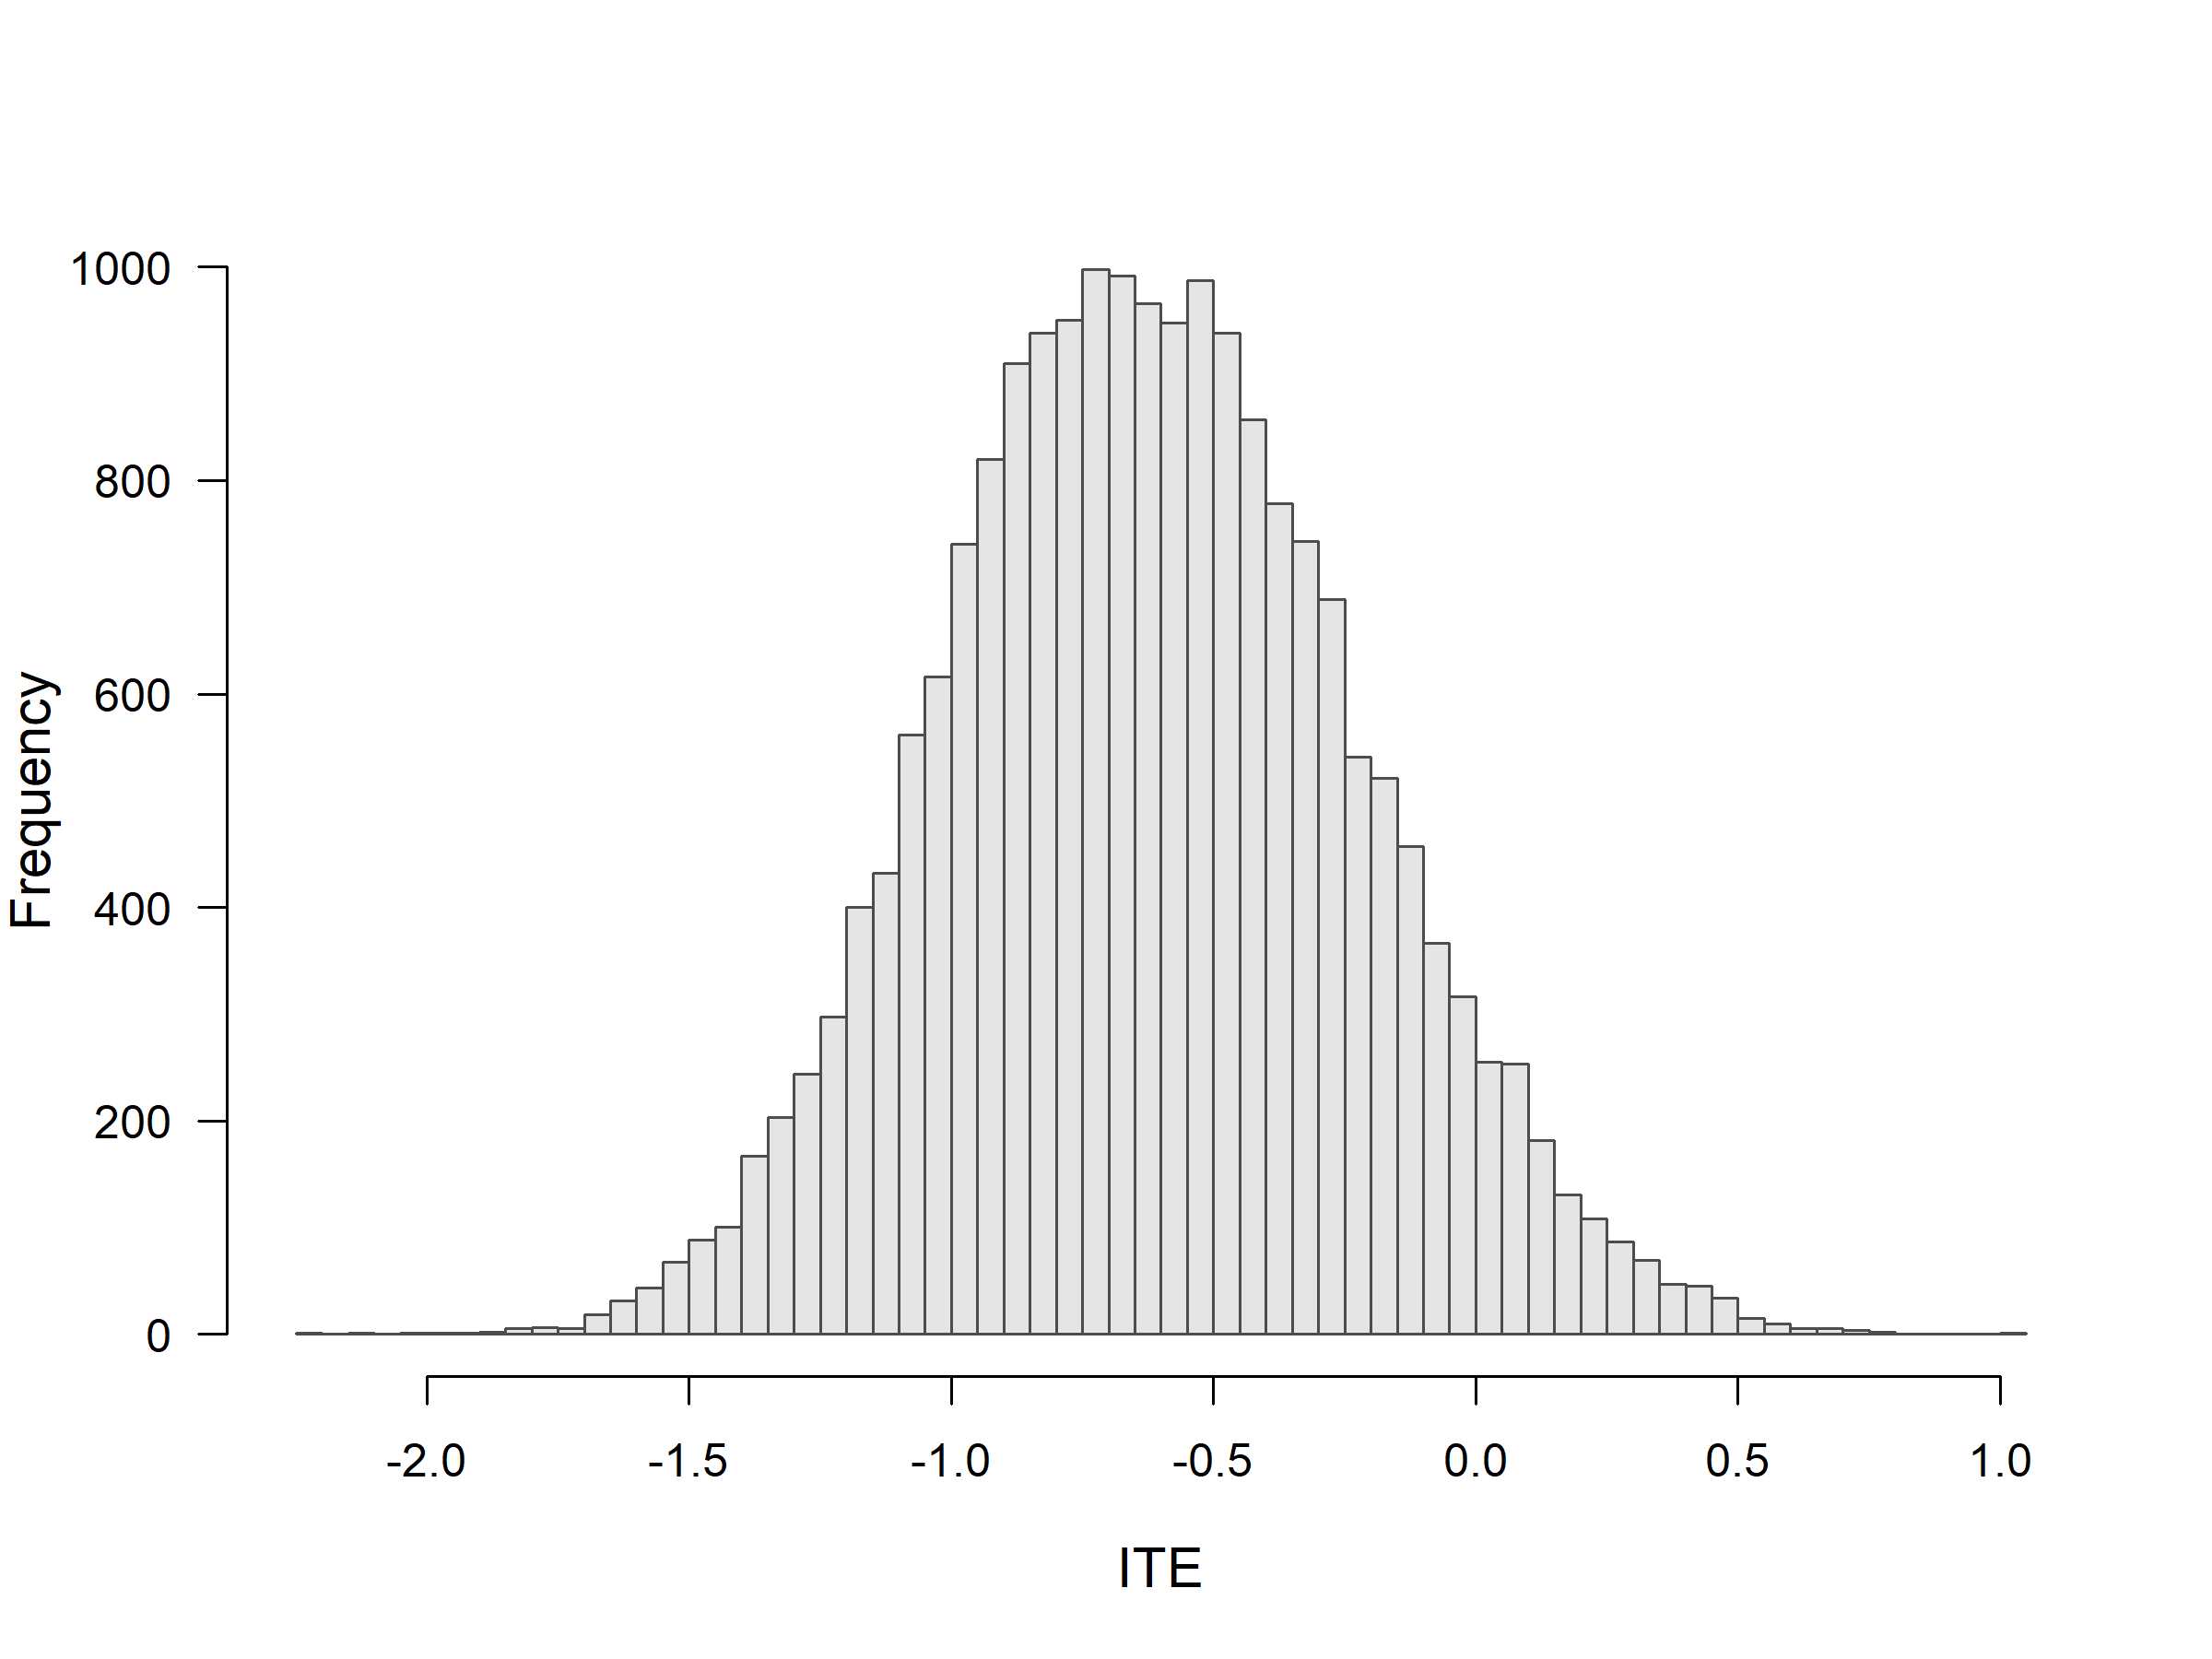
\includegraphics[width=0.7\textwidth]{img/results/observ_scenario1_ite_distribution_dgp.png}
\caption{True ITE distribution resulting from the DGP for Scenario (1), which includes both direct and interaction effects. The true ITEs are identical for each individual in the observational and RCT settings, as they are based on the potential outcomes under both treatment conditions.}
\label{fig:scenario1_ite_distribution_dgp}
\end{figure}



\begin{figure}[htbp]
\centering
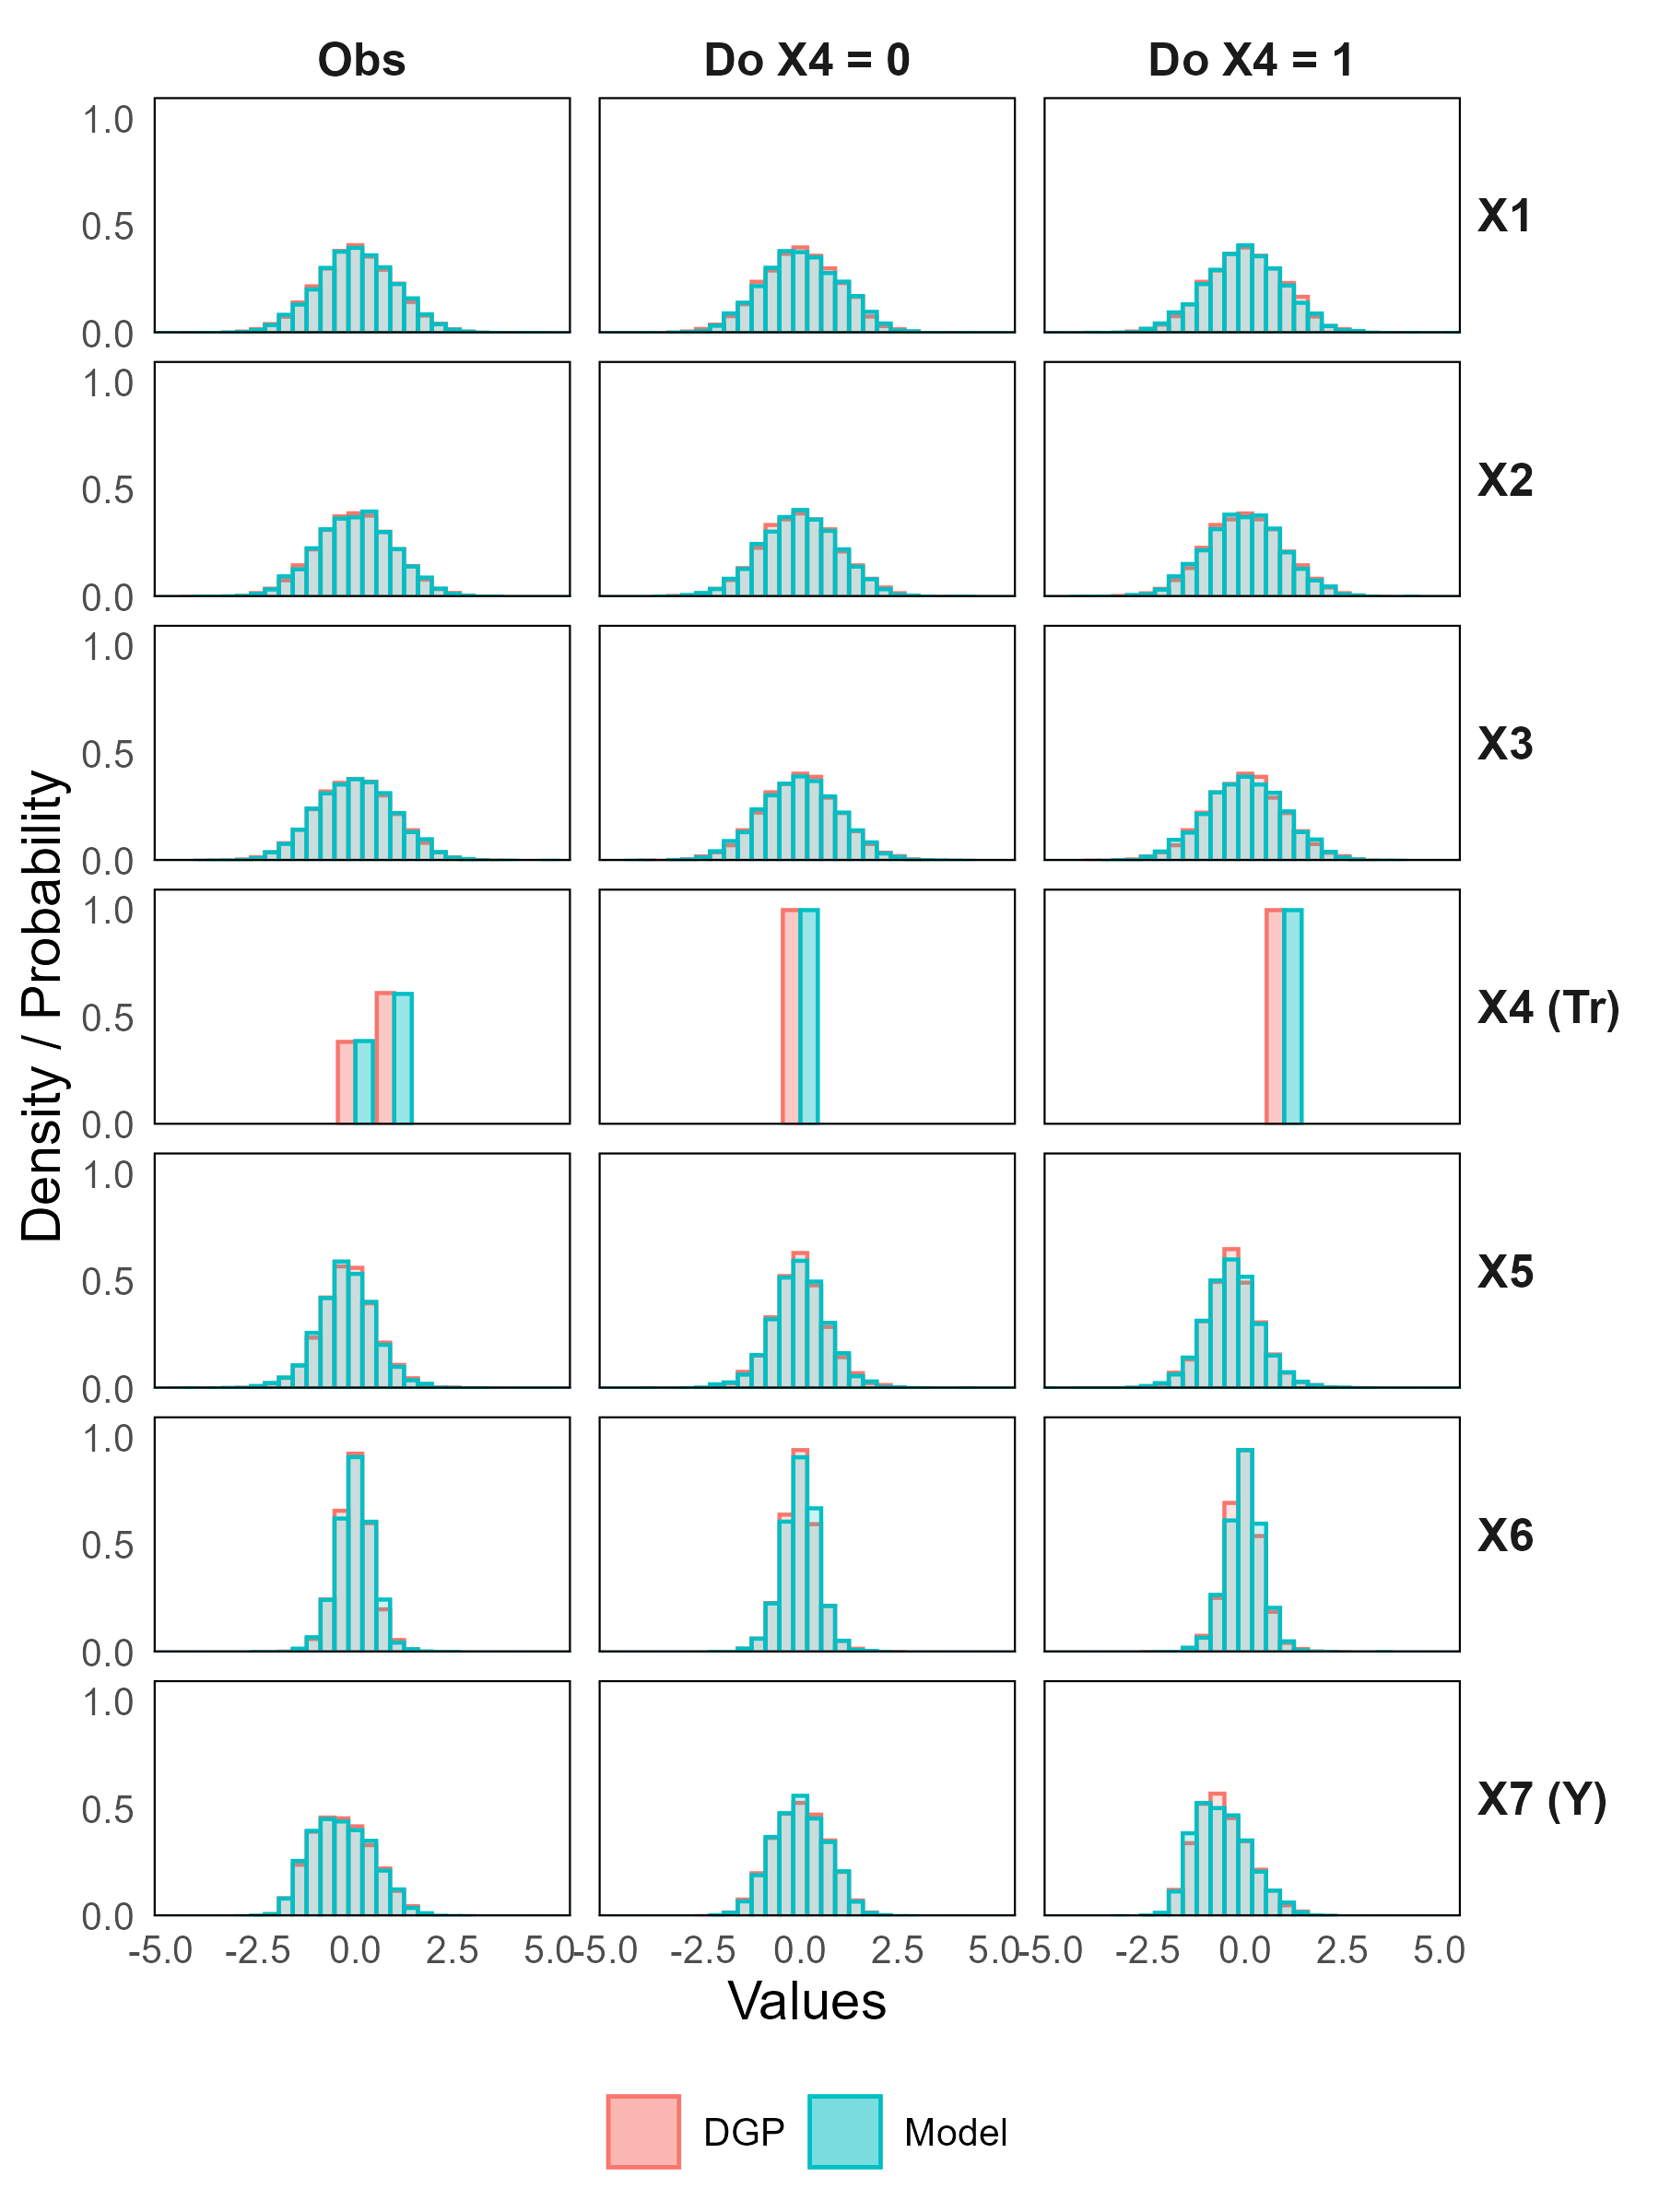
\includegraphics[width=0.45\textwidth]{img/results/observ_scenario1_sampling_distributions_vertical.png}
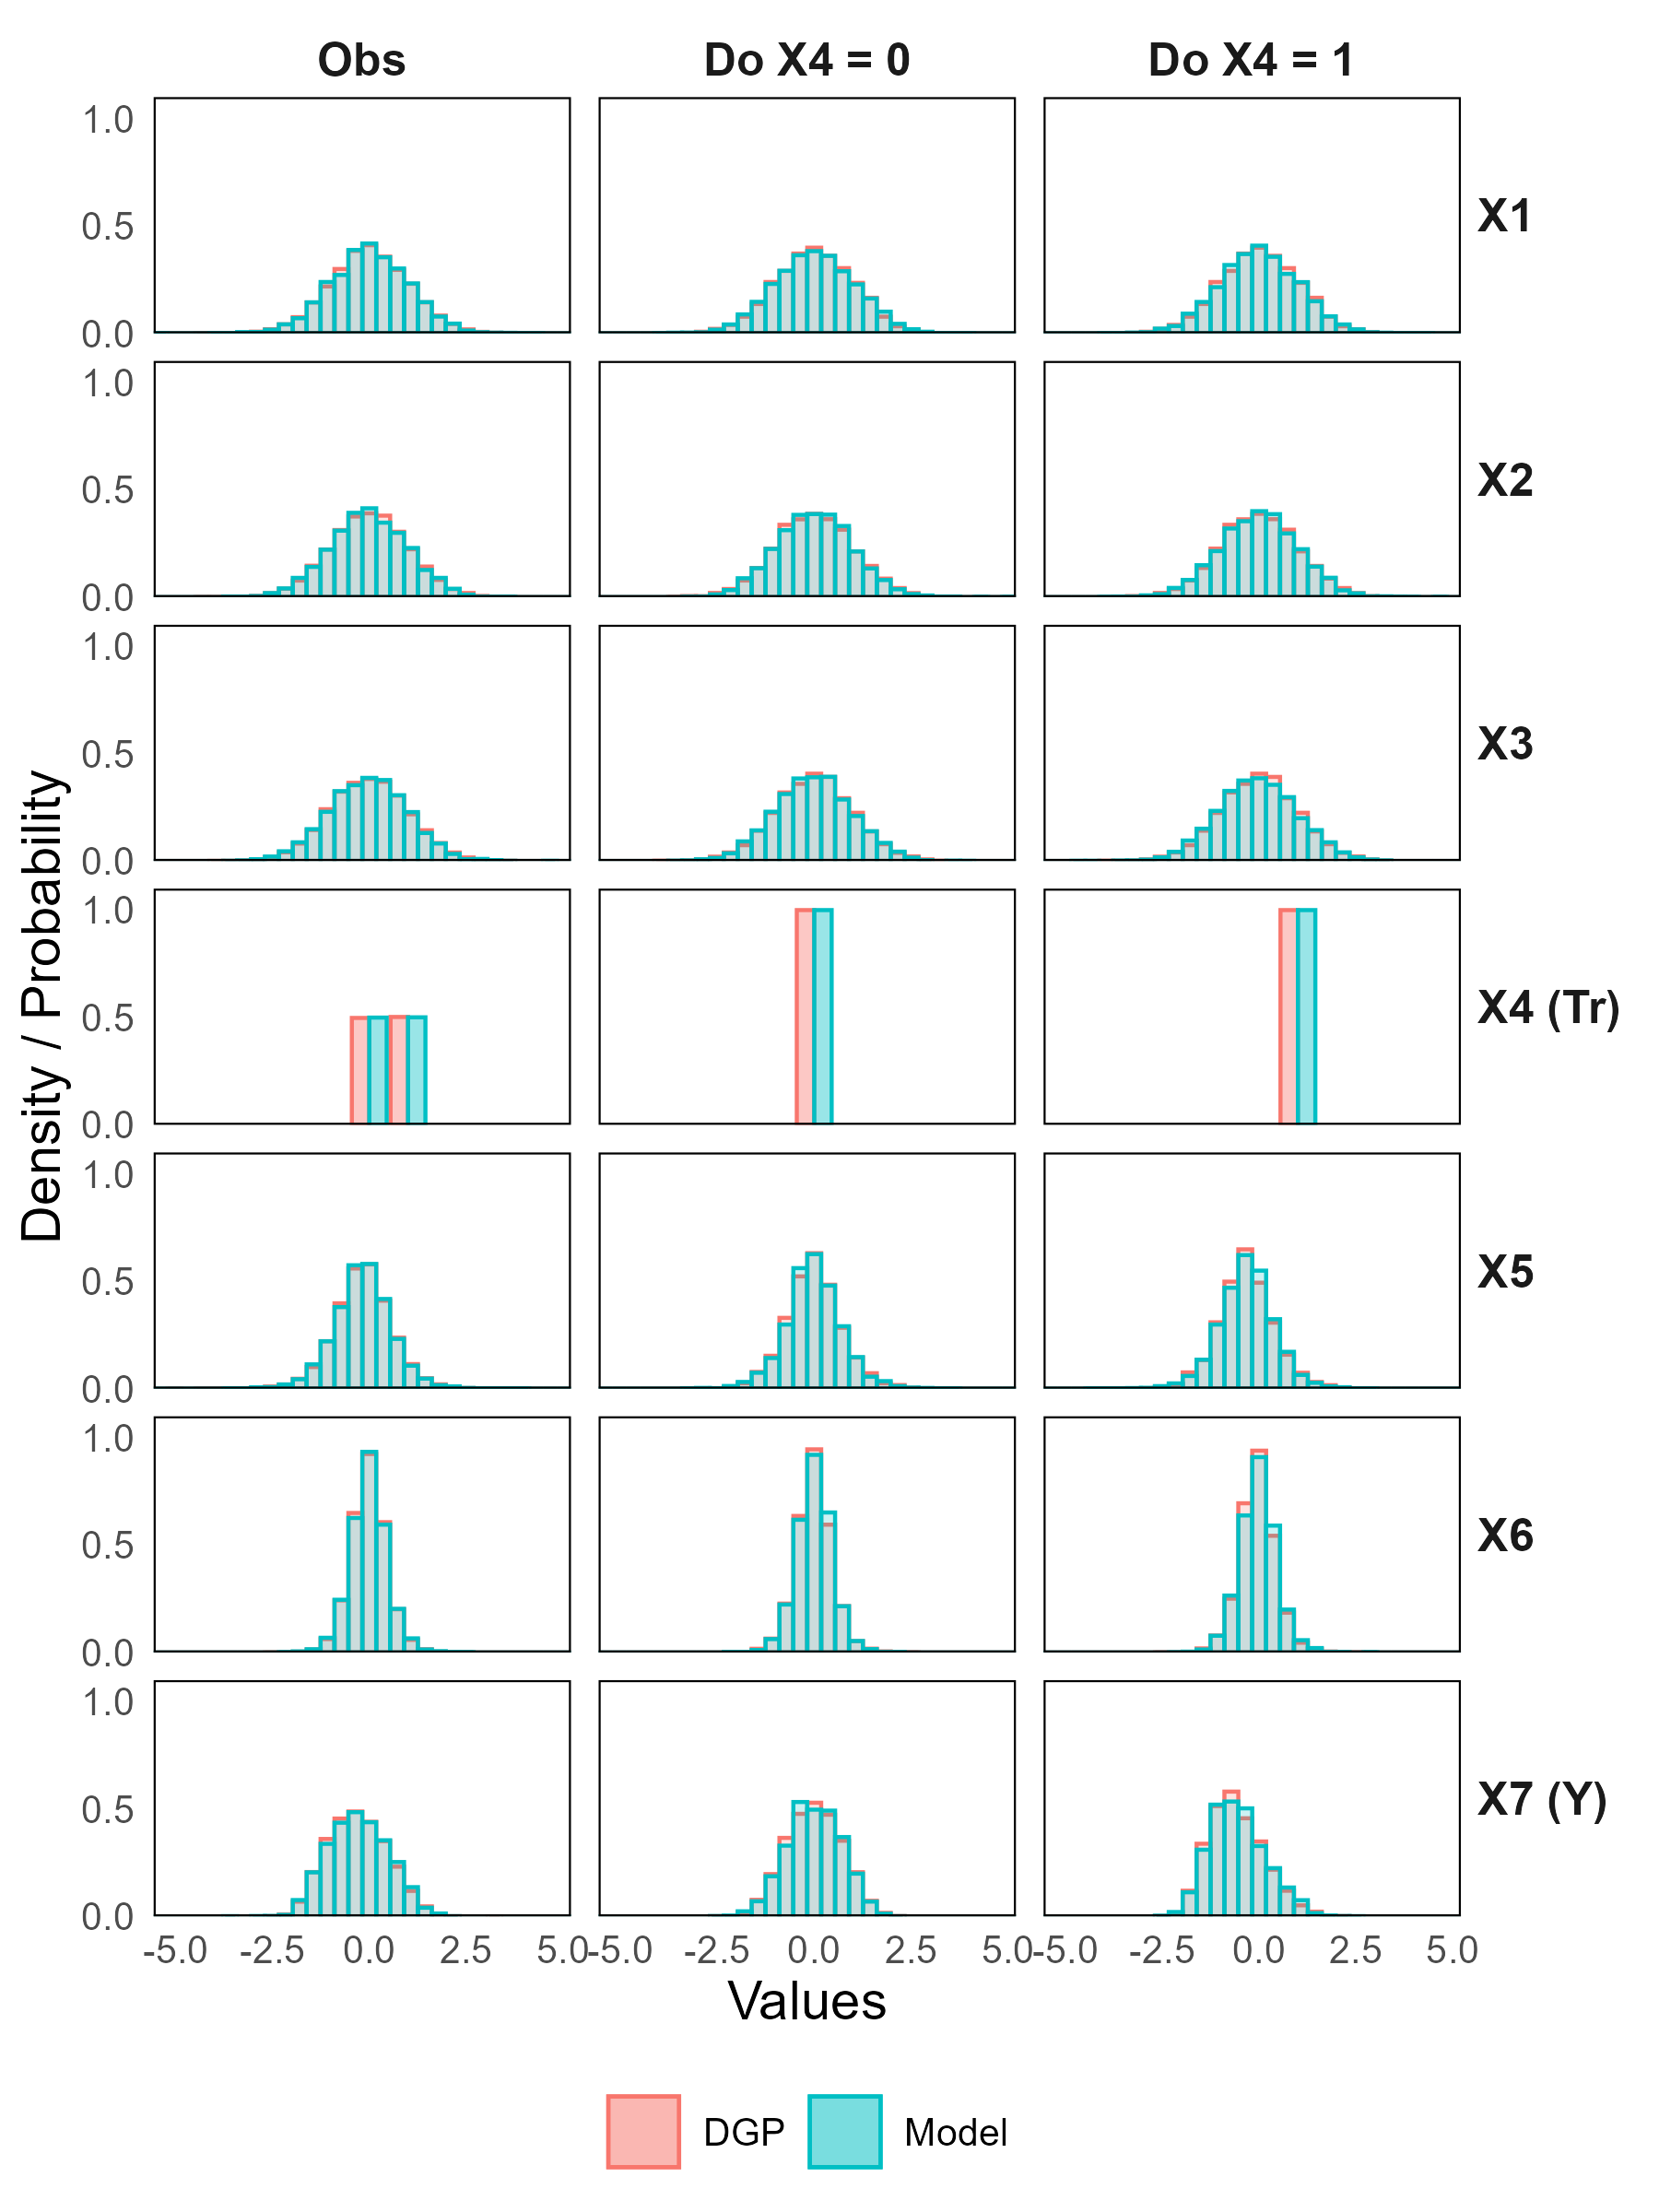
\includegraphics[width=0.45\textwidth]{img/results/rct_scenario1_sampling_distributions_vertical.png}
\caption{Marginal distributions of variables from the DGP and from samples generated by the fitted TRAM-DAG for Scenario (1) with direct and interaction effects. Distributions are shown as observed (Obs), under the control intervention (do($X_4 = 0$)), and under the treatment intervention (do($X_4 = 1$)). Left: Observational; Right: RCT setting.}
\label{fig:scenario1_sampling_distributions_vertical}
\end{figure}


\begin{figure}[htbp]
\centering
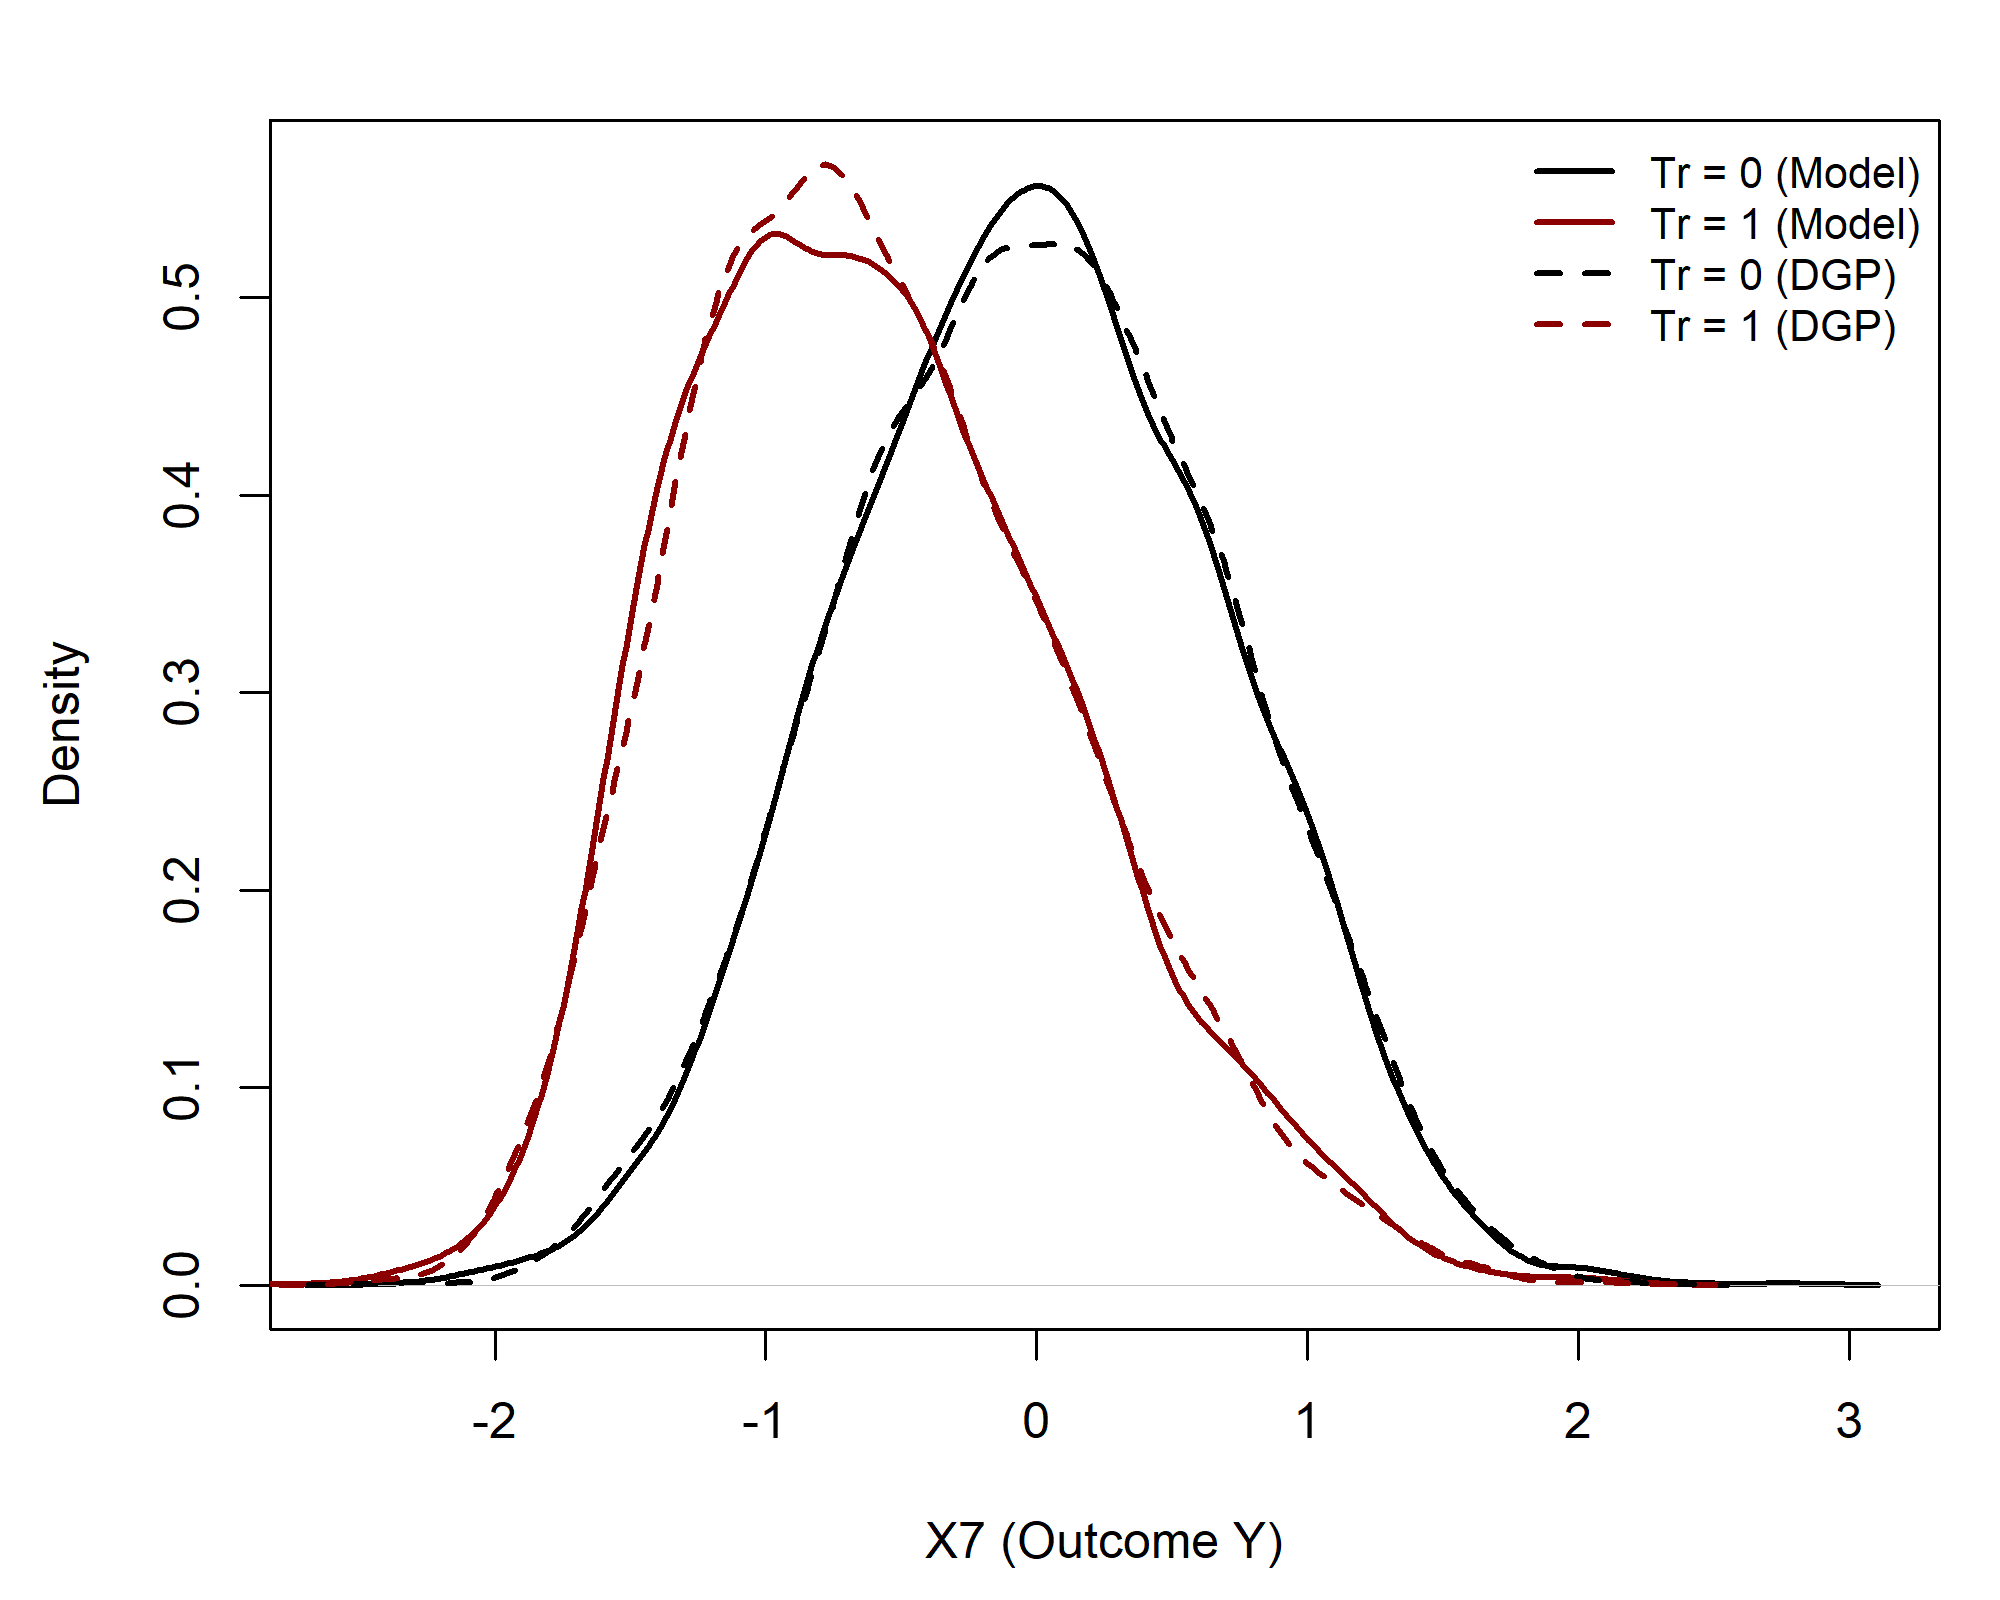
\includegraphics[width=0.45\textwidth]{img/results/observ_scenario1_X7_treatment_densities.png}
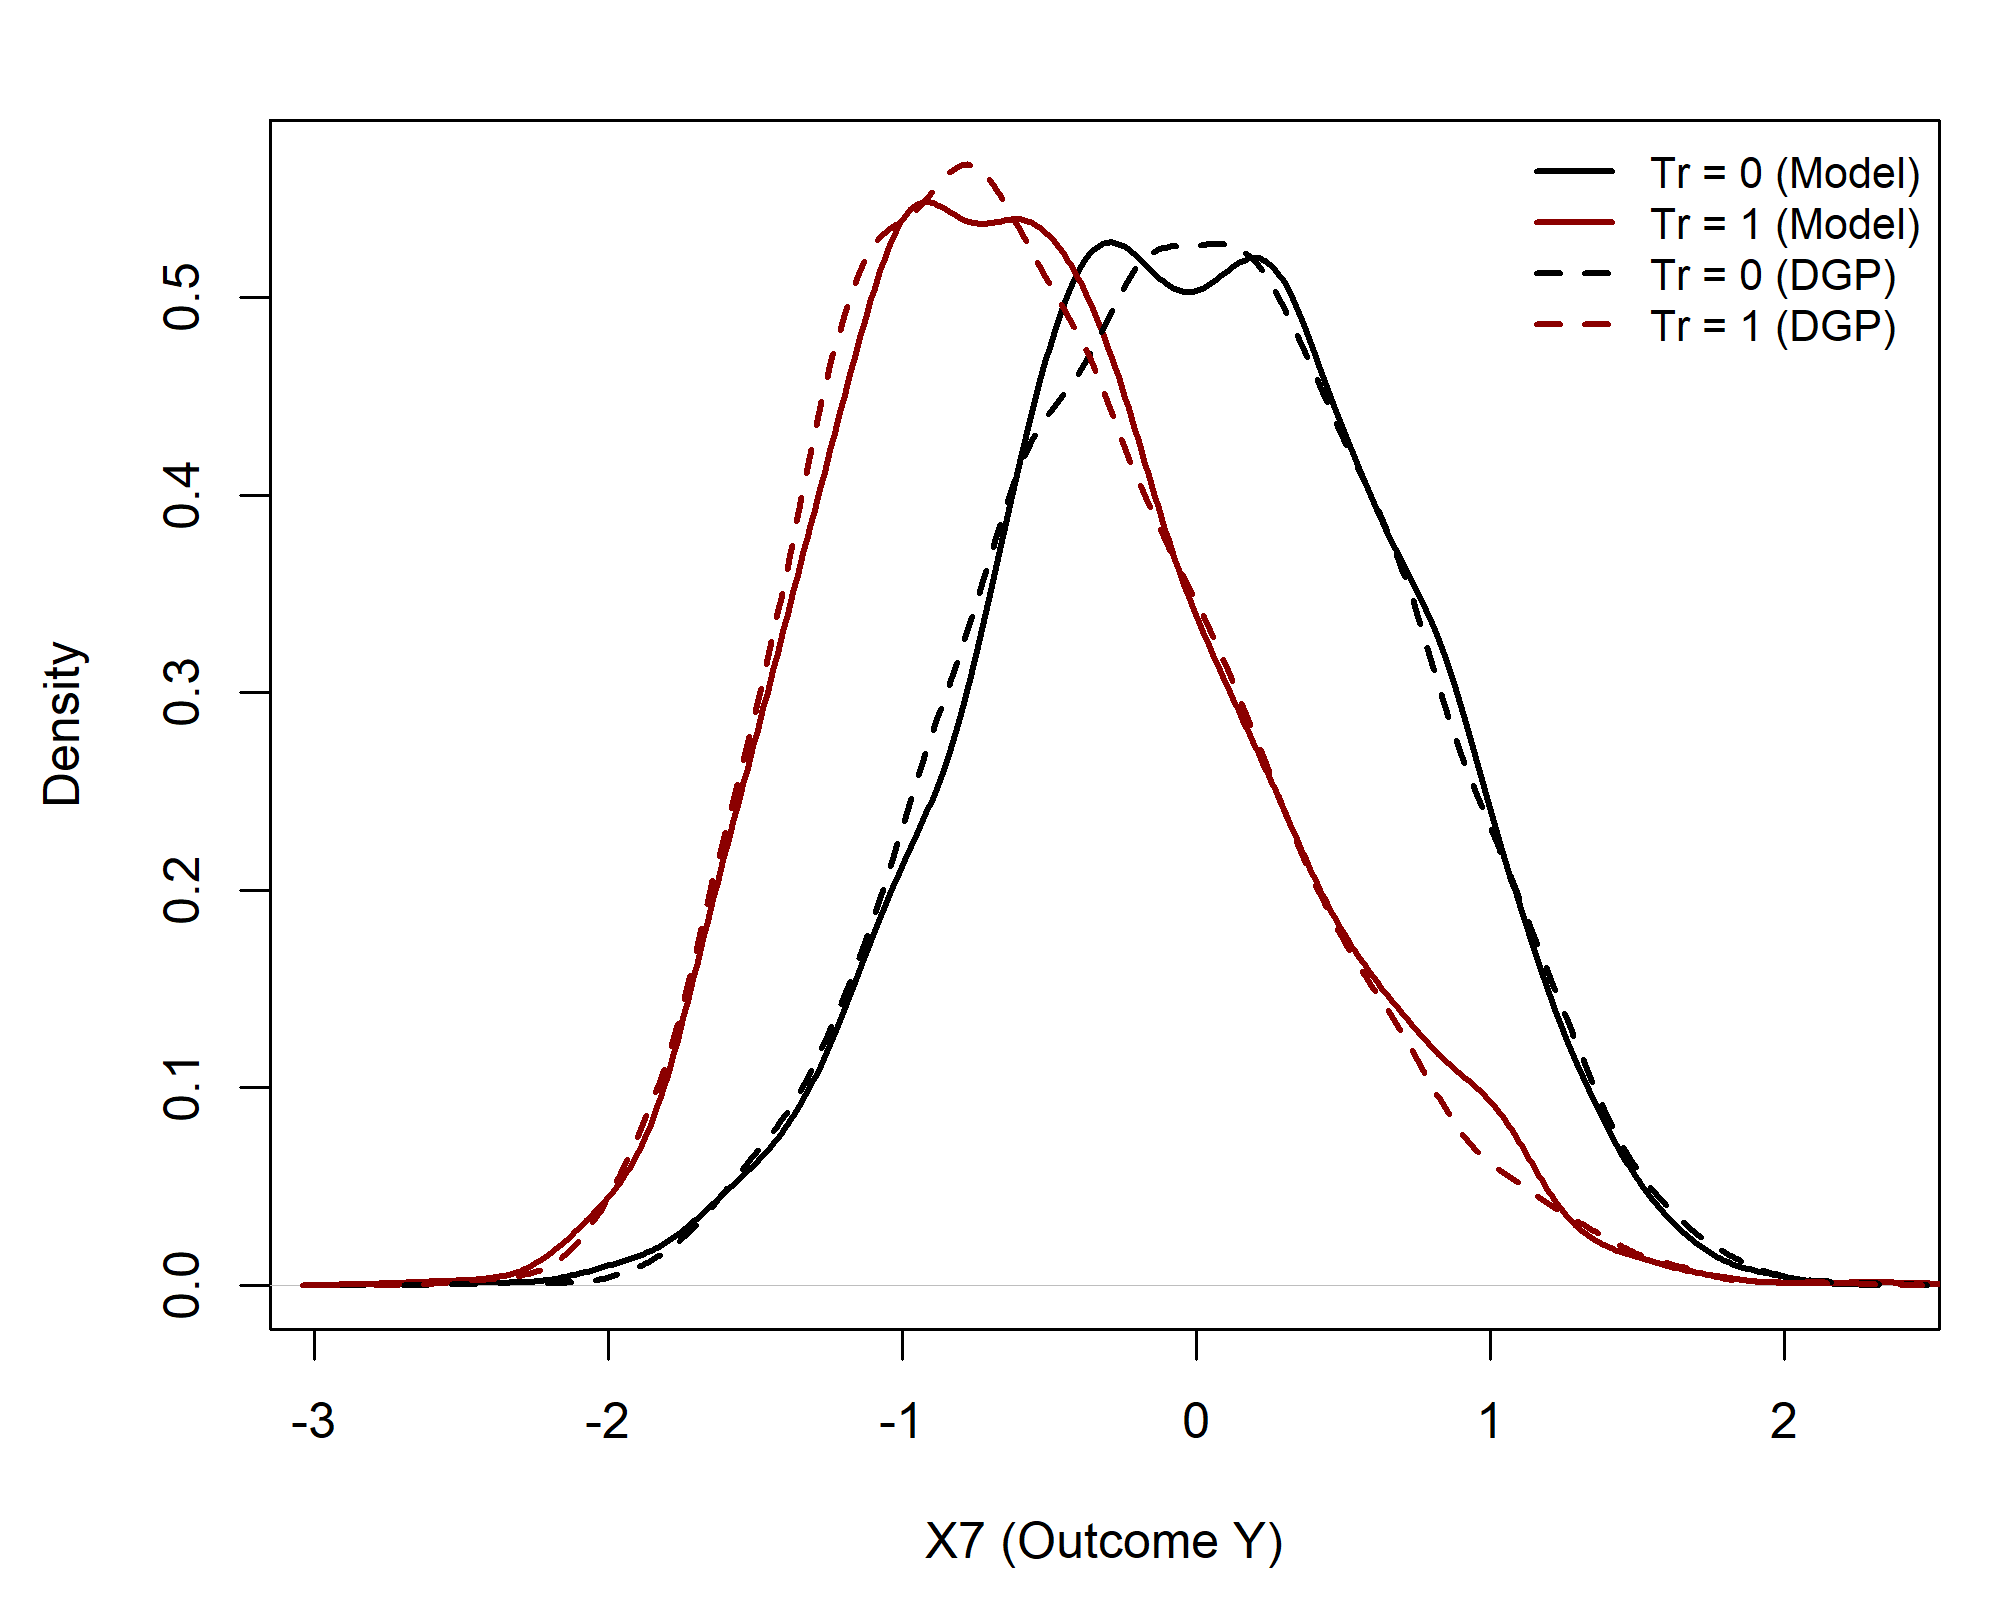
\includegraphics[width=0.45\textwidth]{img/results/rct_scenario1_X7_treatment_densities.png}
\caption{Distributions of the outcome variable ($X_7$) under control and treatment interventions for Scenario (1), which includes both direct and interaction effects. This plot provides a more detailed view of the $X_7$ panels shown under do($X_4=0$) and do($X_4=1$) in Figure~\ref{fig:scenario1_sampling_distributions_vertical}. Left: Observational; Right: RCT setting.}
\label{fig:scenario1_outcome_distributions}
\end{figure}




\begin{figure}[htbp]
\centering
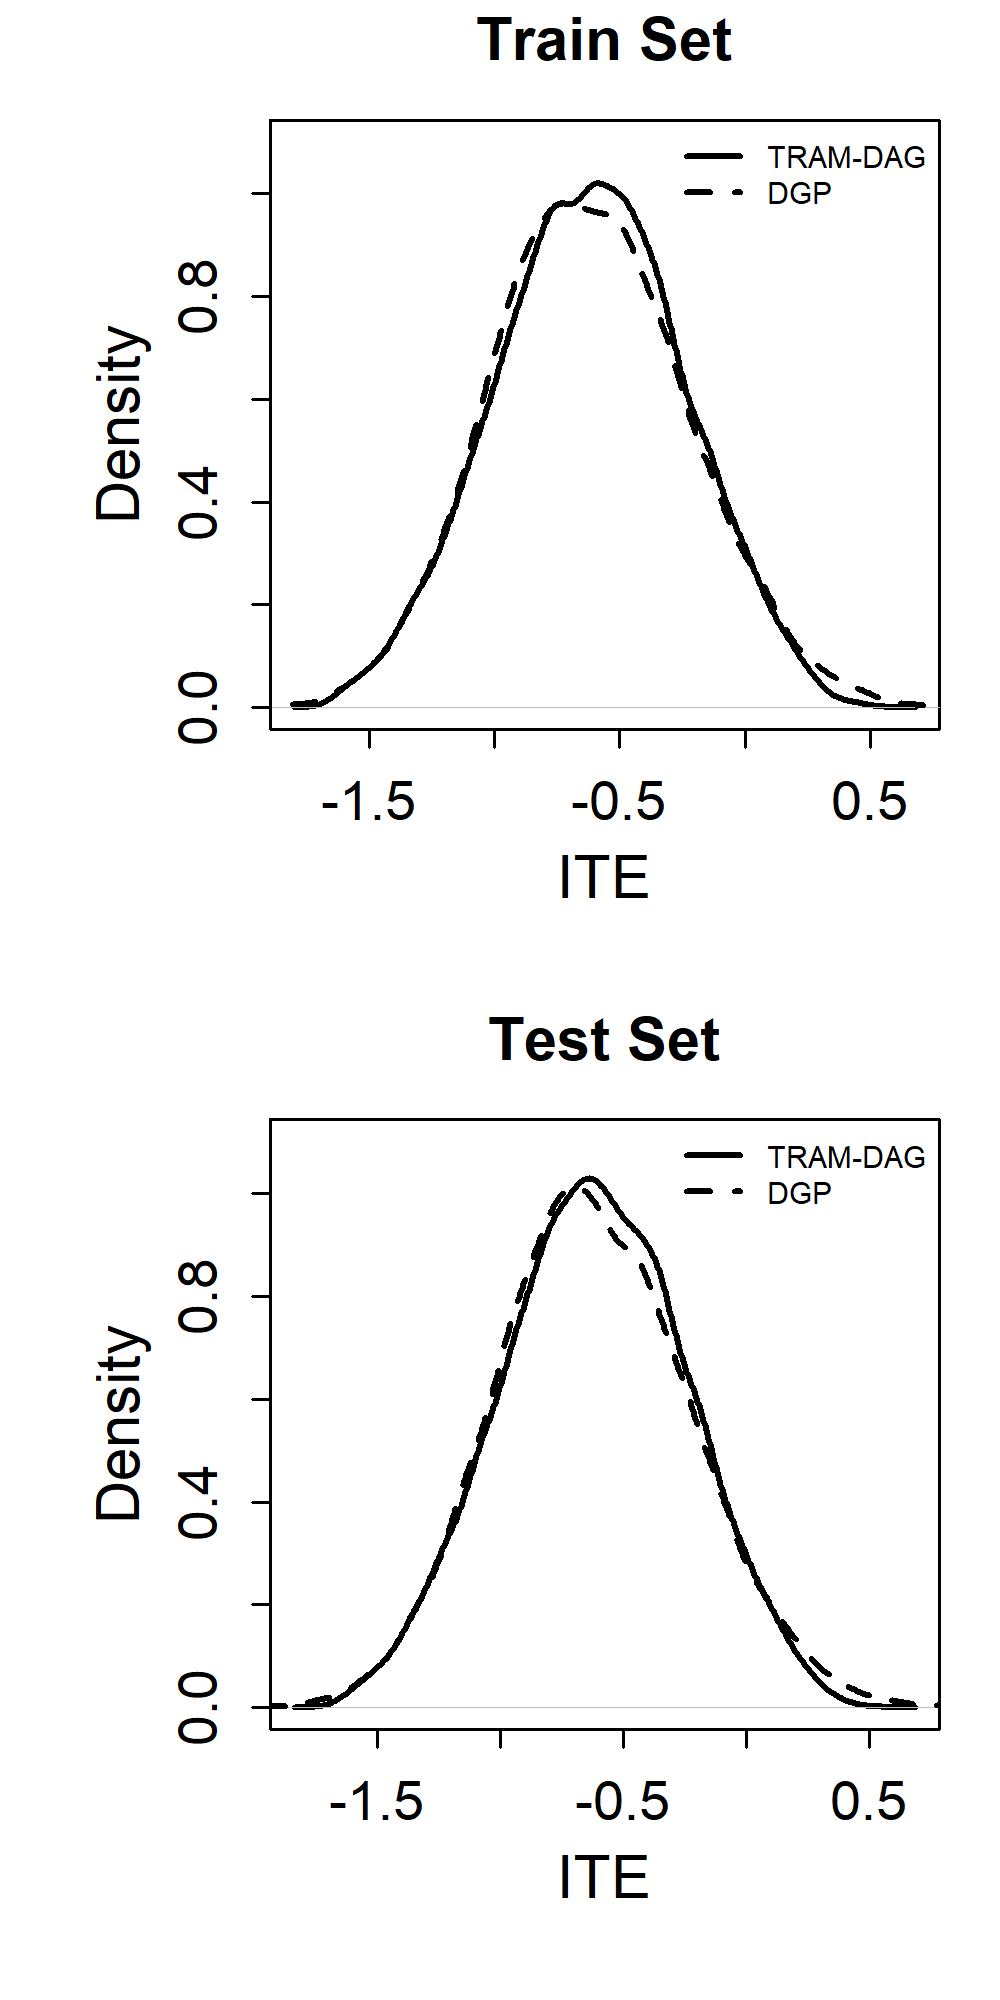
\includegraphics[width=0.33\textwidth]{img/results/observ_scenario1_ITE_densities_train_test.png} 
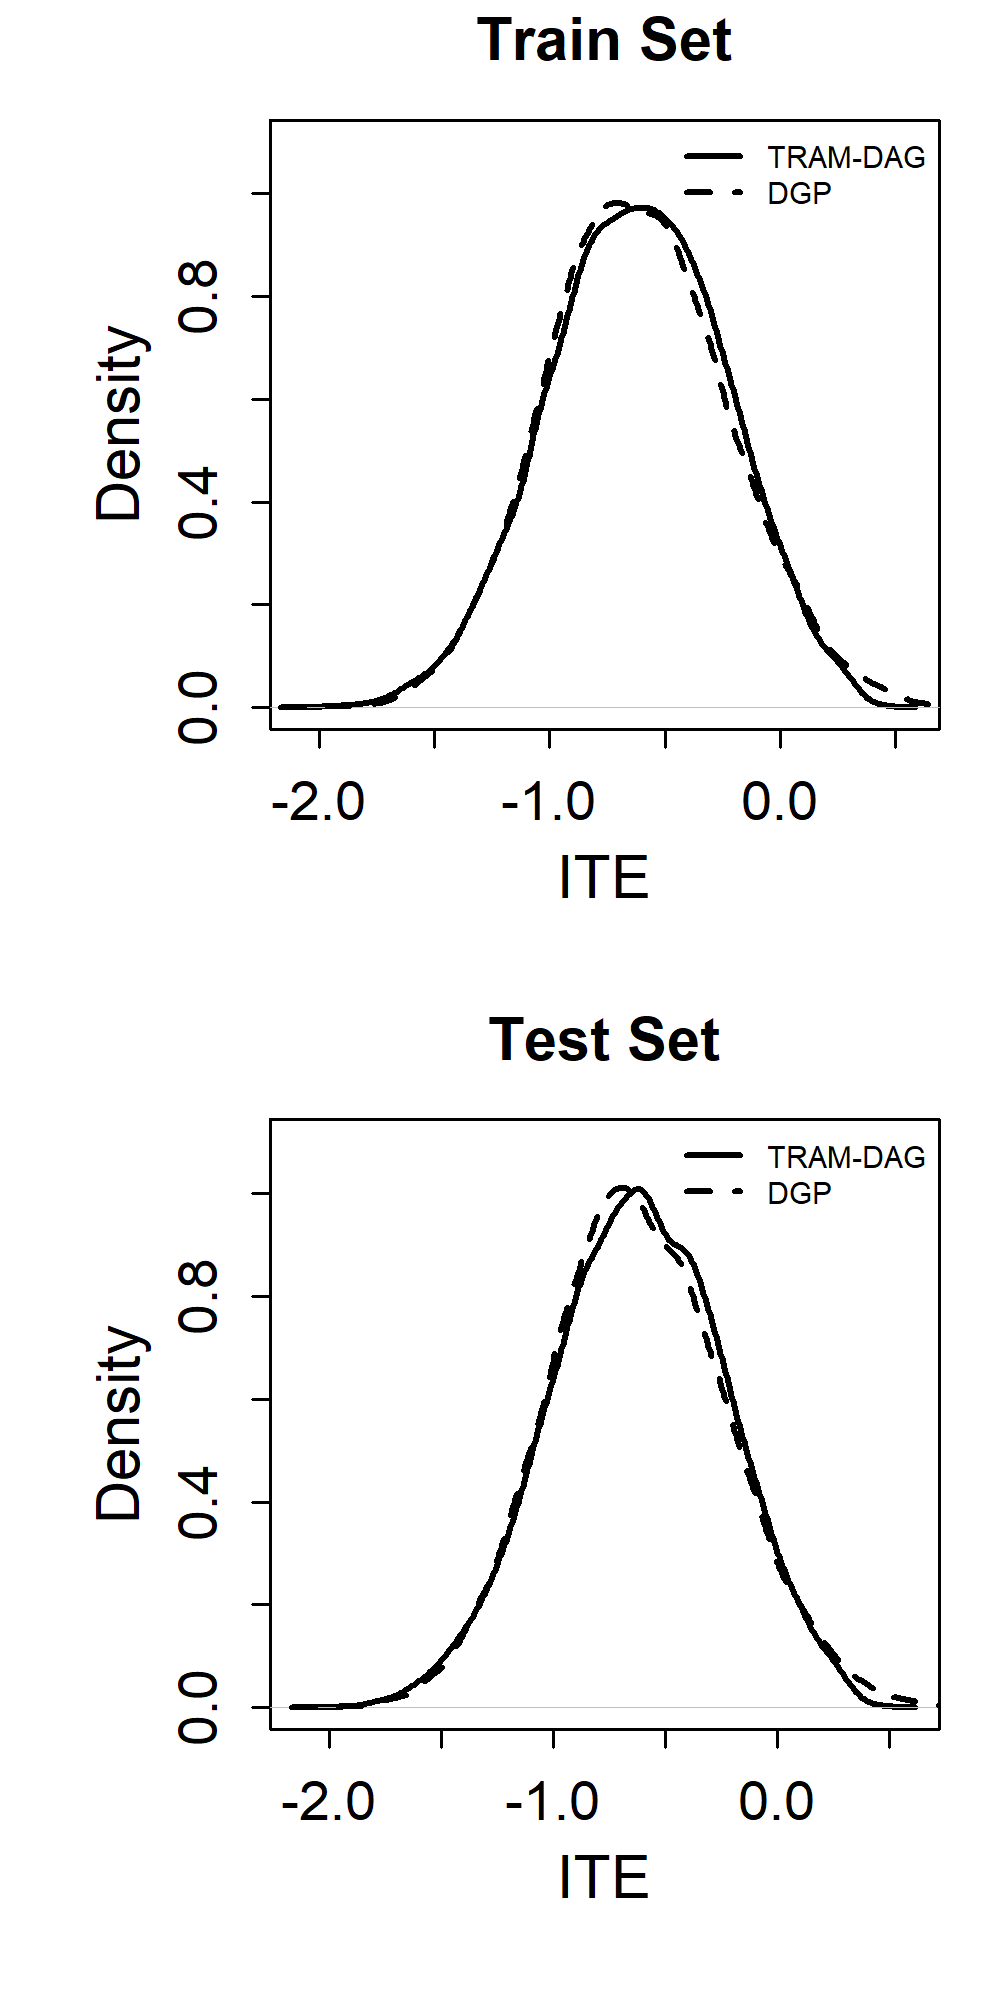
\includegraphics[width=0.33\textwidth]{img/results/rct_scenario1_ITE_densities_train_test.png}
\vspace{-17pt}
\caption{Densities of the estimated ITEs compared to the true ITEs in the training and test datasets for Scenario (1), which includes direct and interaction effects. Left: Observational; Right: RCT setting.}
\label{fig:scenario1_ite_densities_train_test}
\end{figure}






\begin{figure}[htbp]
\centering
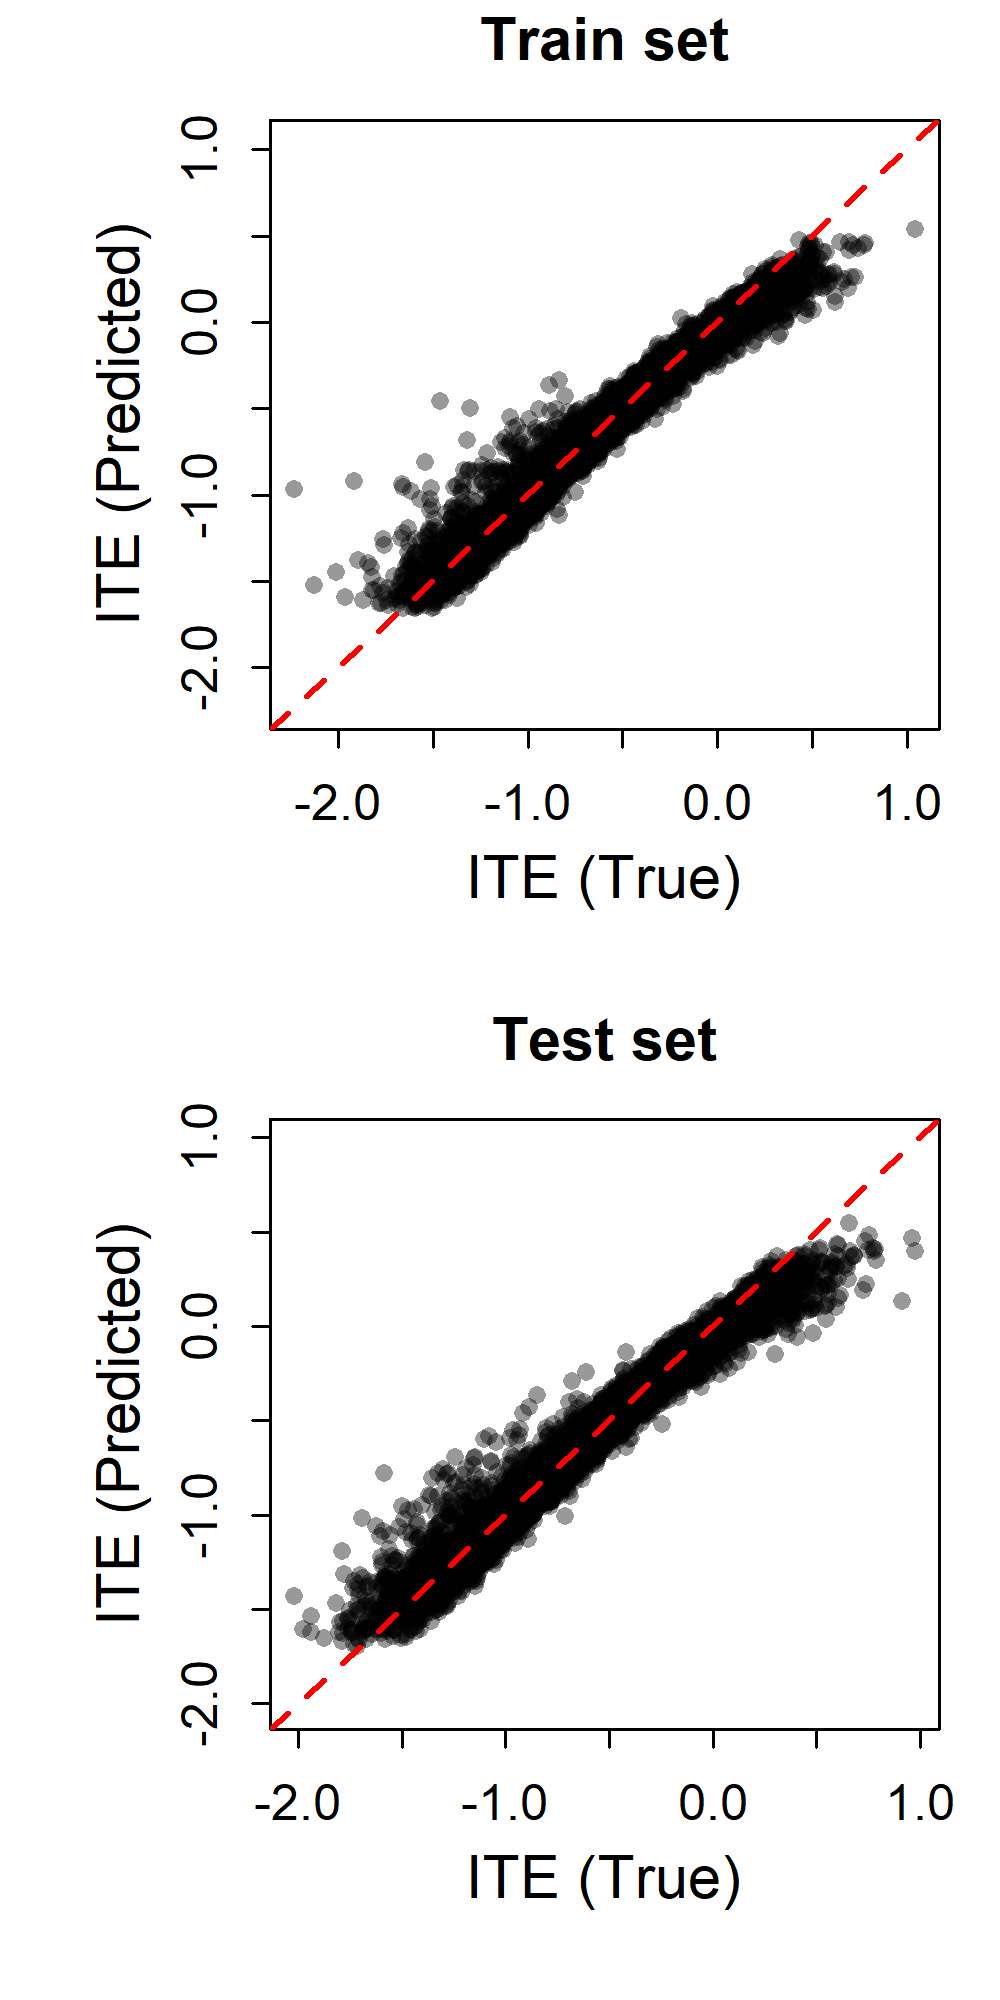
\includegraphics[width=0.33\textwidth]{img/results/observ_scenario1_ITE_scatter_train_test.png} 
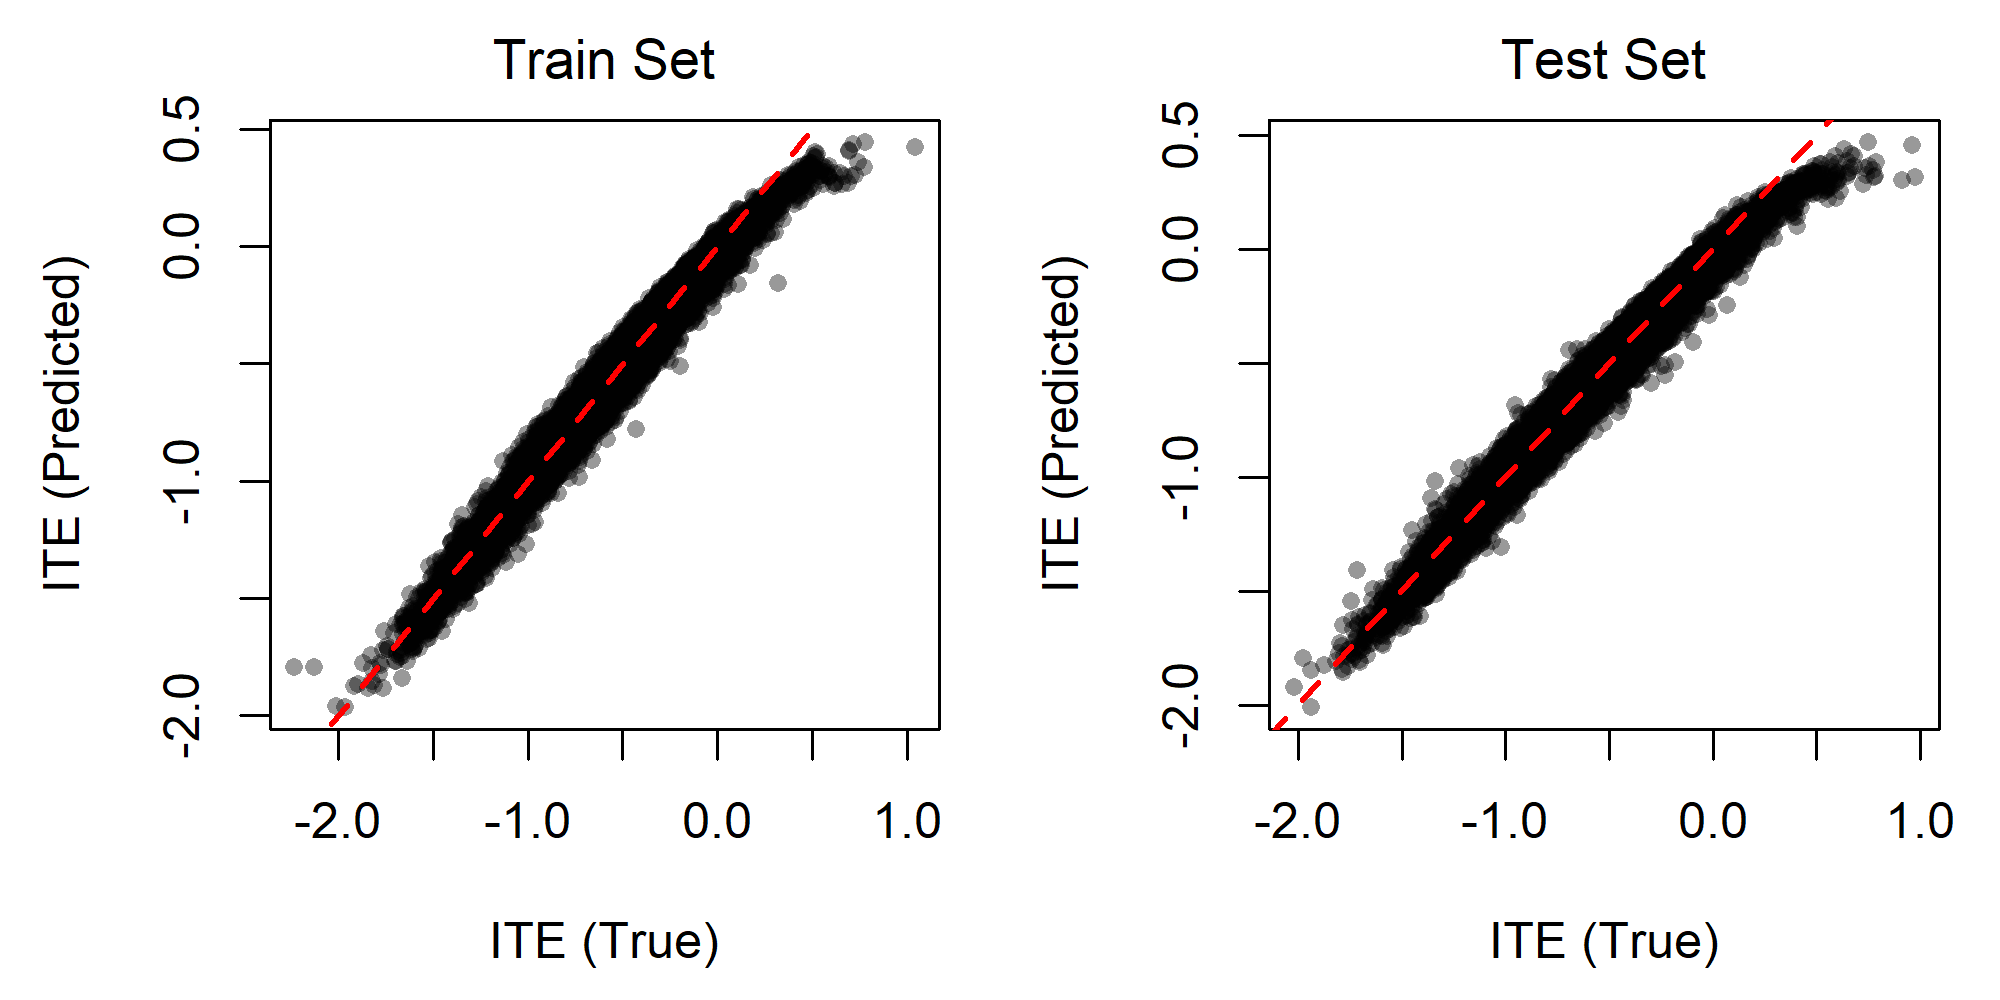
\includegraphics[width=0.33\textwidth]{img/results/rct_scenario1_ITE_scatter_train_test.png}
\vspace{-17pt}
\caption{Scatterplots of estimated ITEs vs. true ITEs in the training and test datasets for Scenario (1), which includes direct and interaction effects. Left: Observational; Right: RCT setting.}
\label{fig:scenario1_ite_scatter_train_test}
\end{figure}



% 
% \begin{figure}[htbp]
% \centering
% 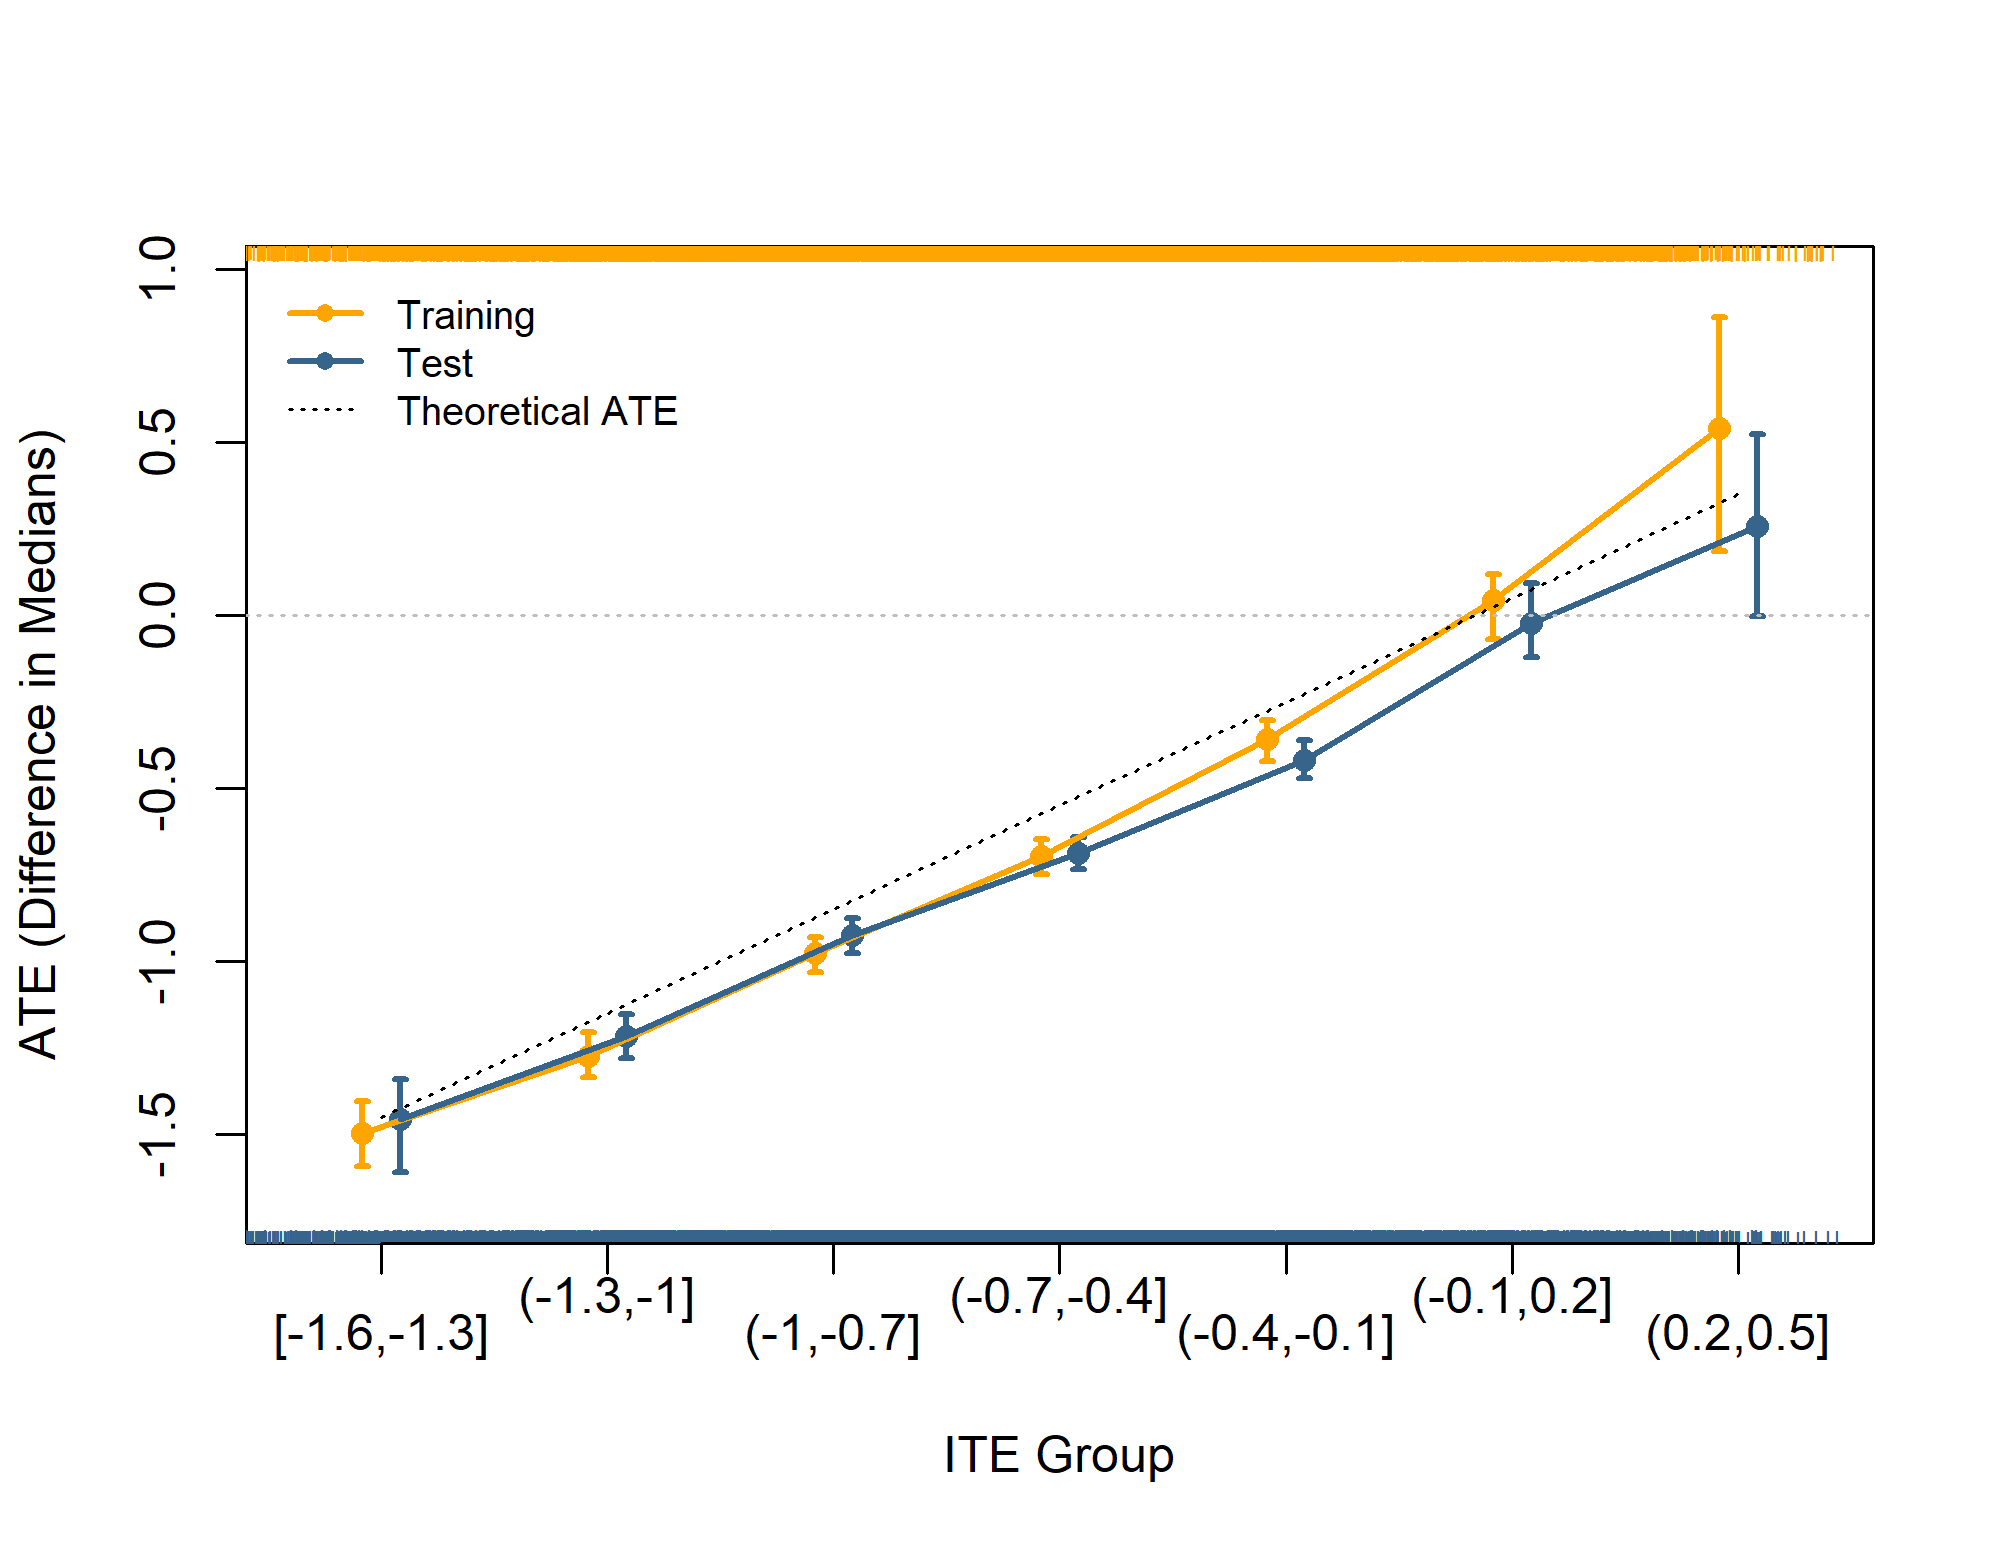
\includegraphics[width=0.45\textwidth]{img/results/observ_scenario1_ITE_ATE.png}
% 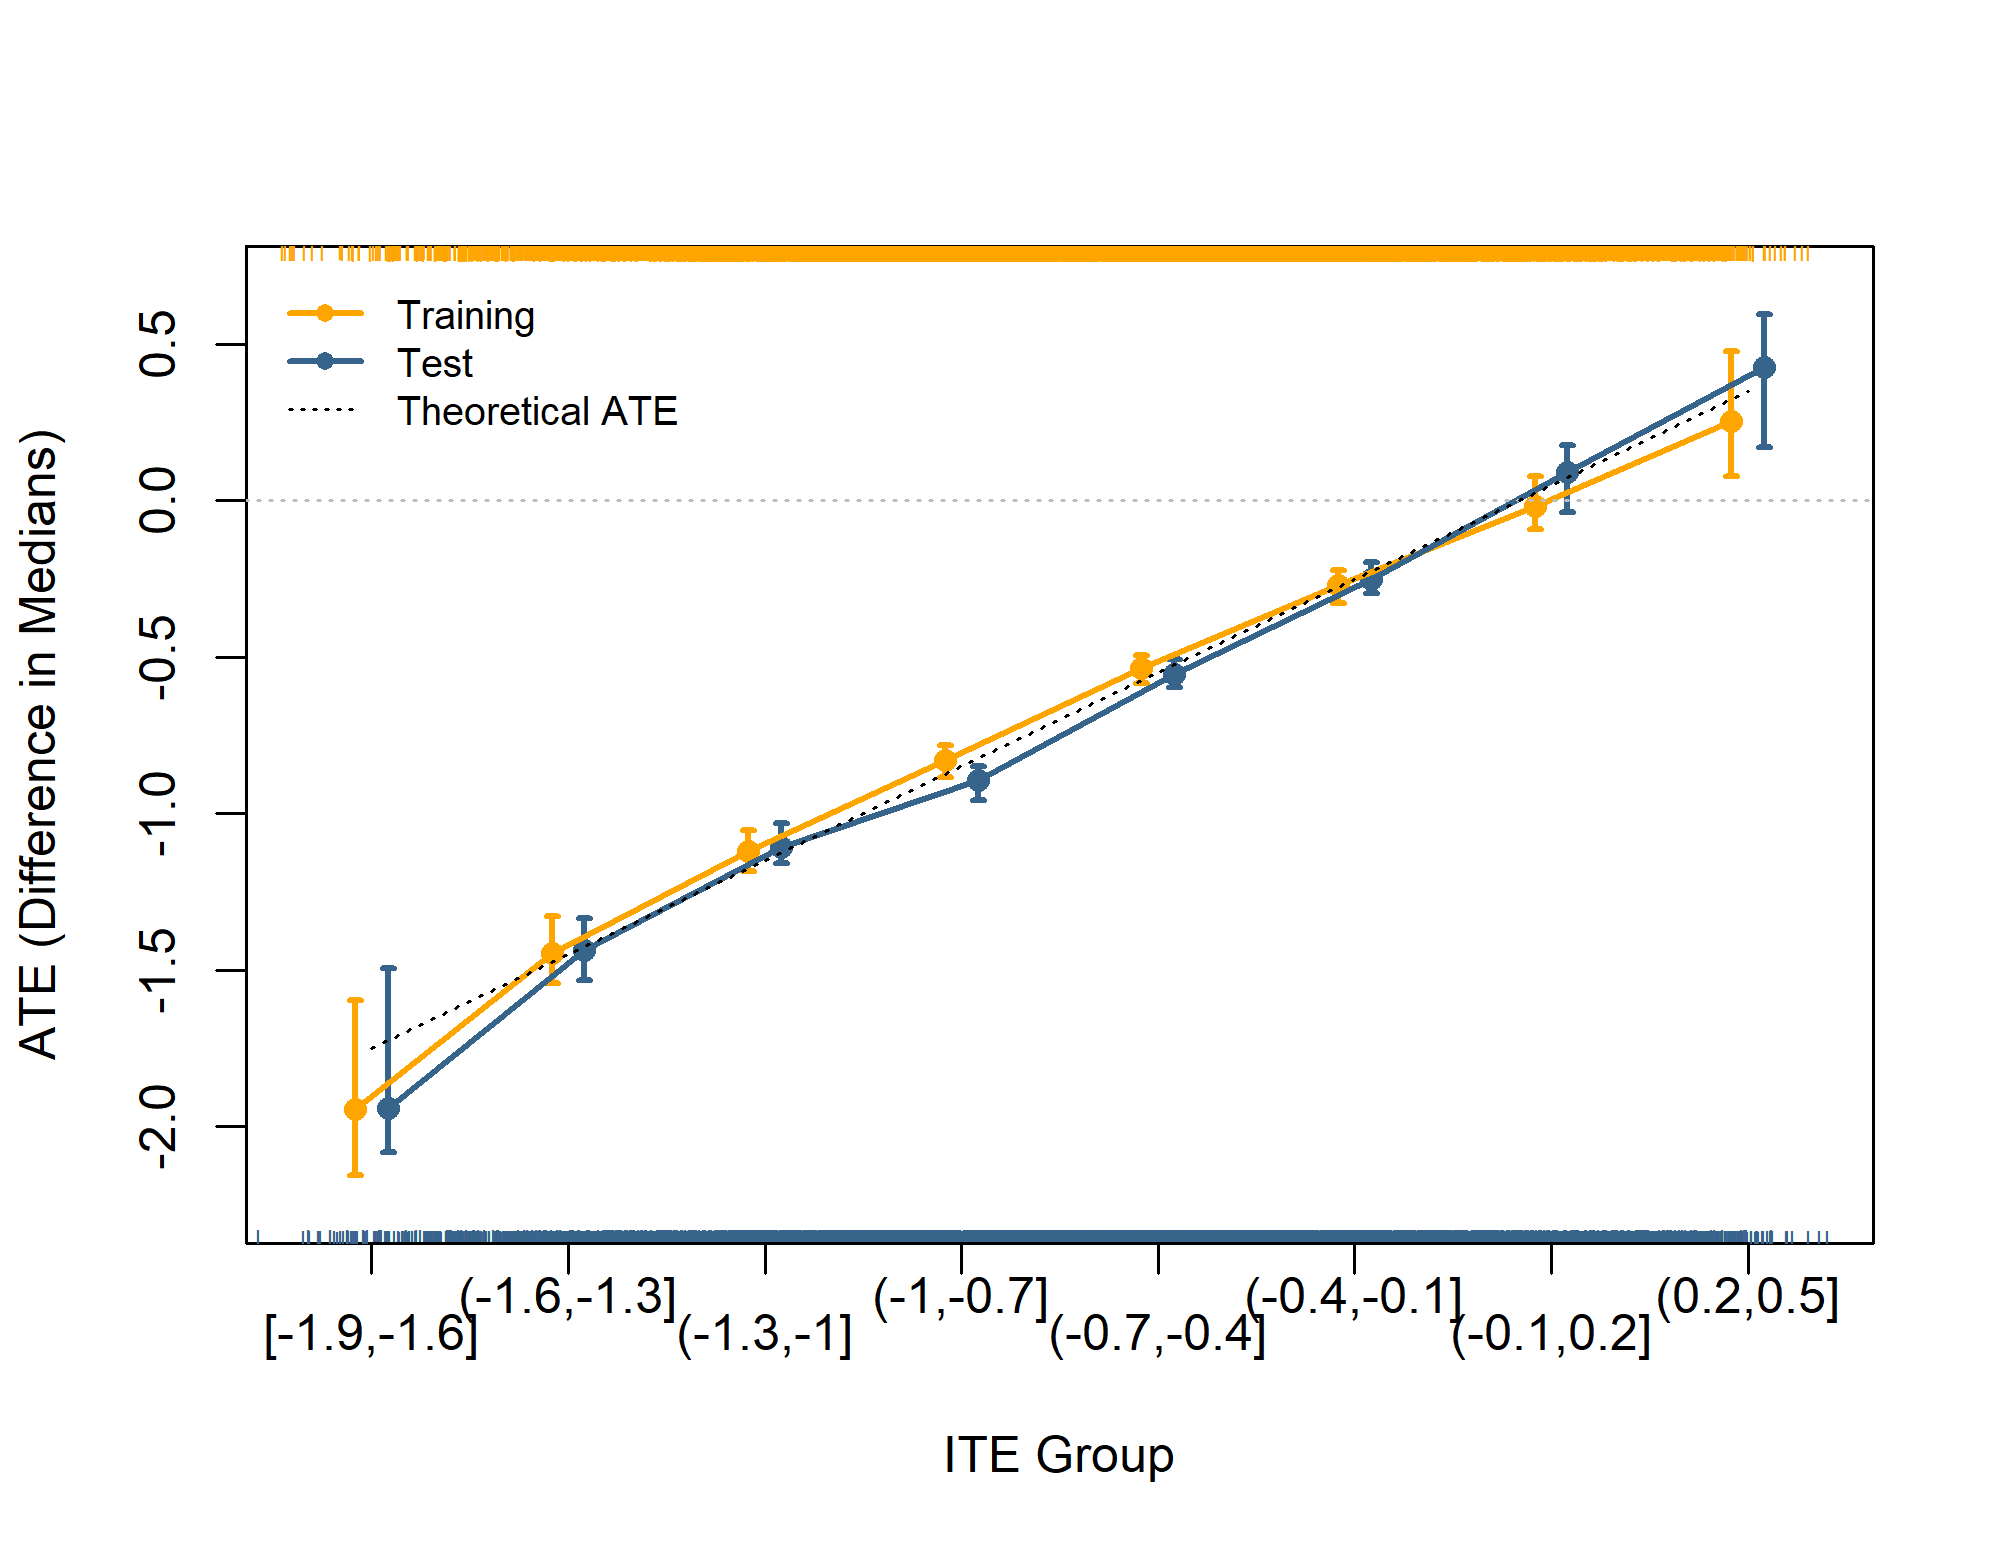
\includegraphics[width=0.45\textwidth]{img/results/rct_scenario1_ITE_ATE.png}
% \caption{ITE-ATE plots for Scenario (1), which includes direct and interaction effects. Individuals are grouped into bins based on their estimated ITEs, and within each bin, the ATE is calculated as the difference in medians of the observed outcomes under the two treatments. 95\% bootstrap confidence intervals indicate the uncertainty. Left: Observational; Right: RCT setting.}
% \label{fig:scenario1_ite_cATE}
% \end{figure}


\begin{figure}[htbp]
\centering
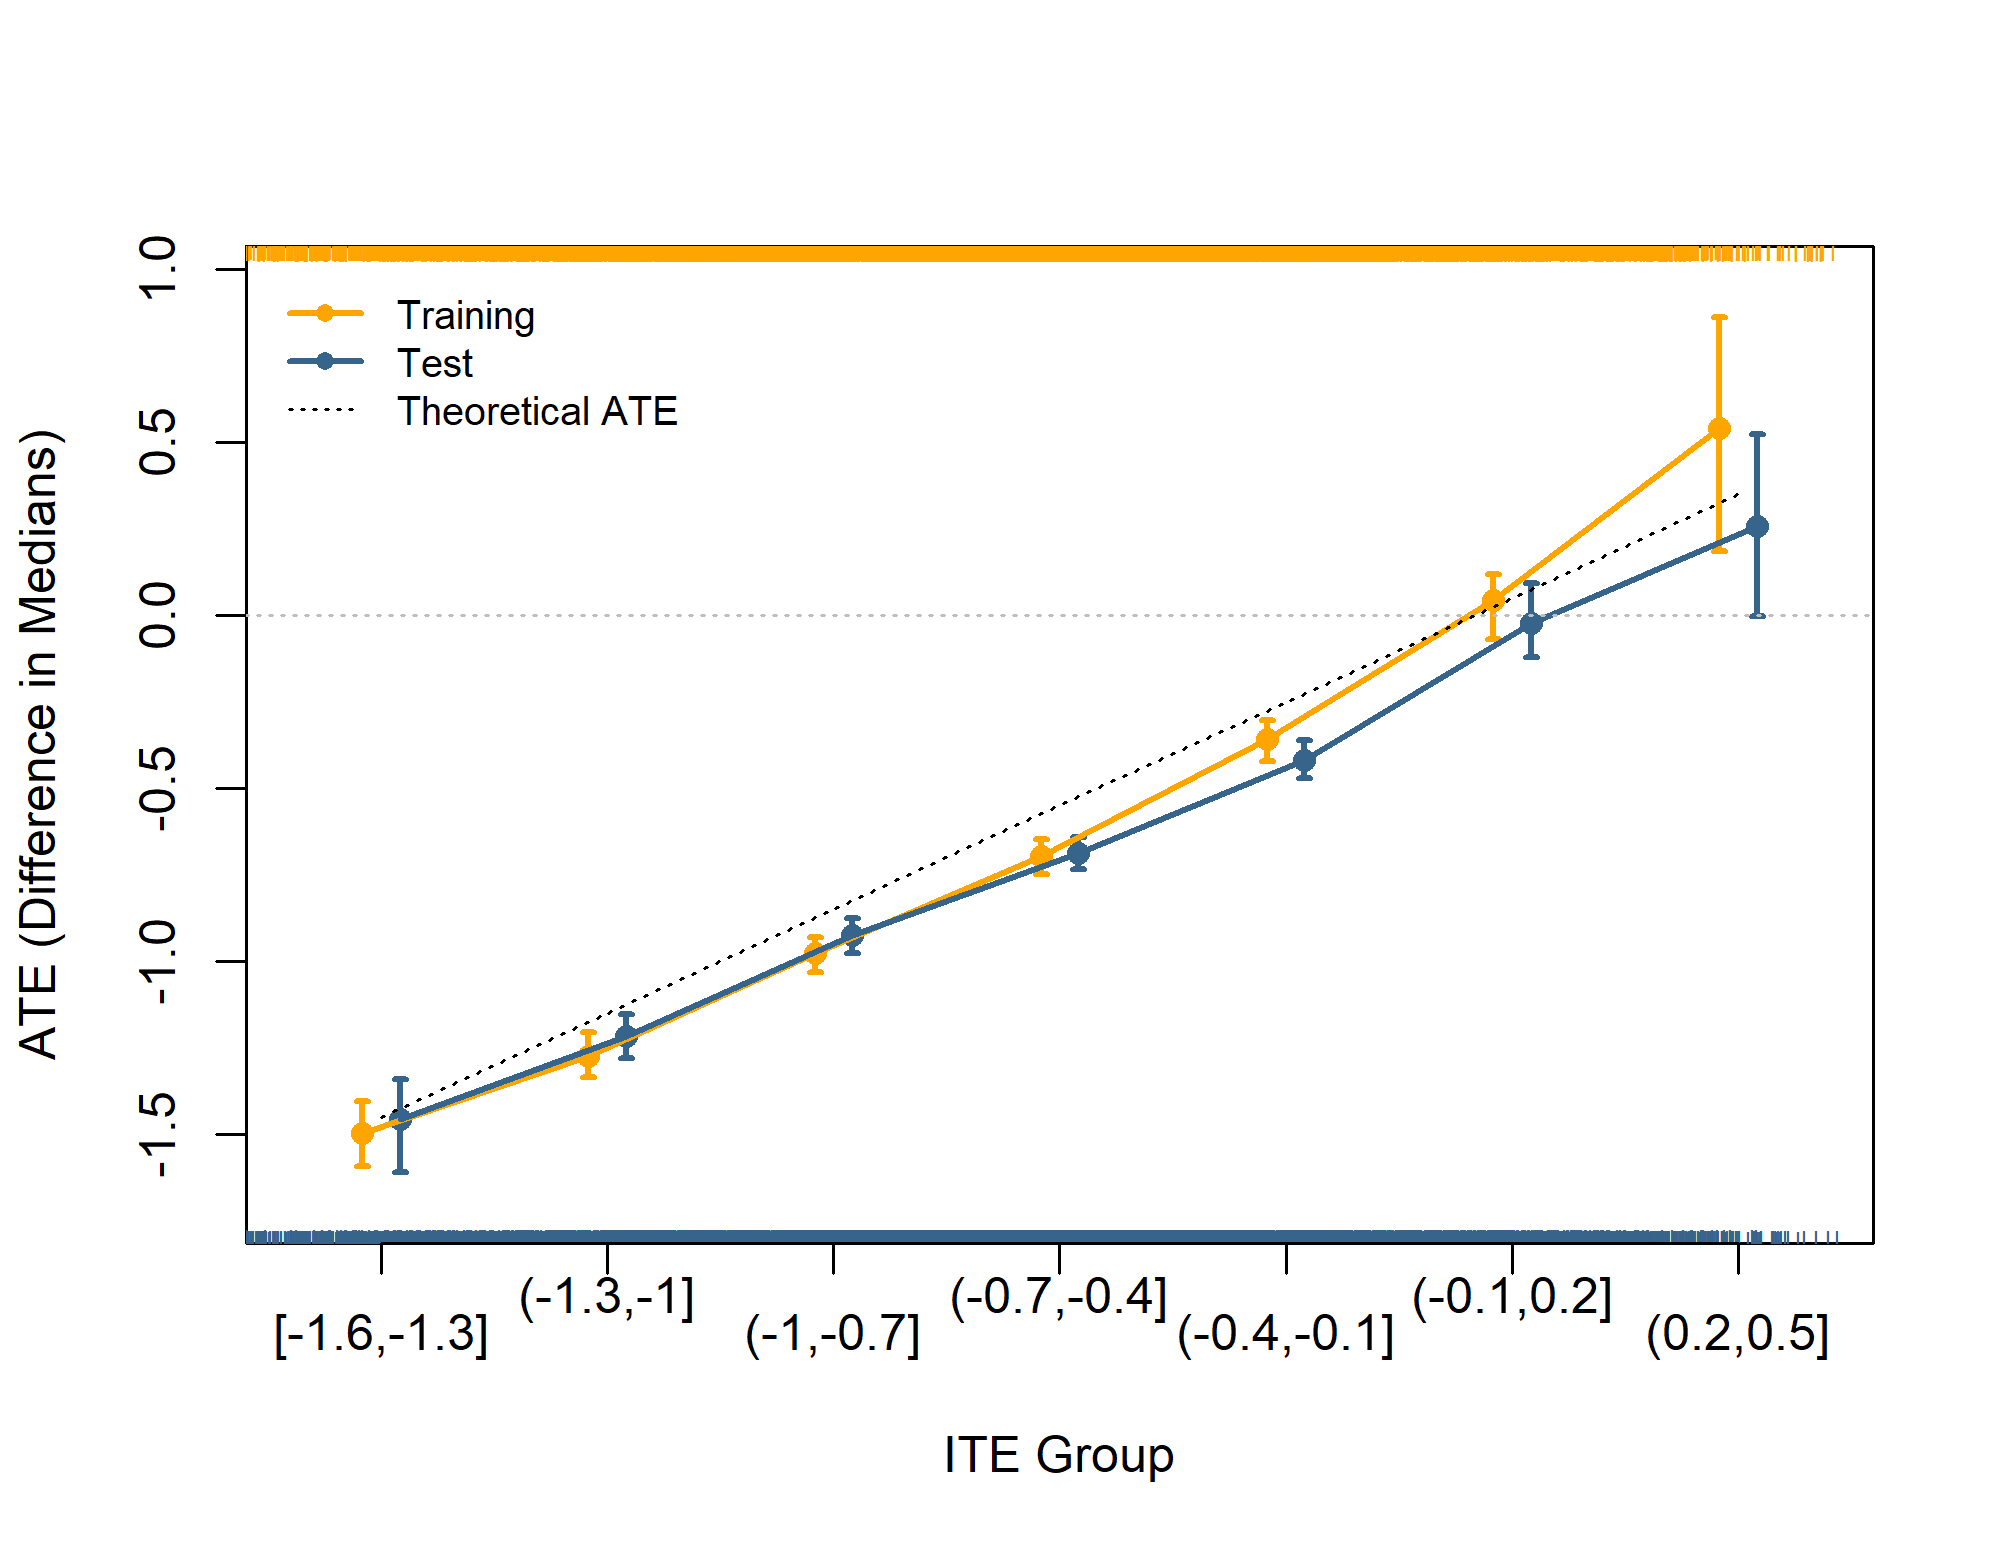
\includegraphics[width=0.8\textwidth]{img/results/observ_scenario1_ITE_ATE.png}
\vspace{-15pt}
\caption{ITE-ATE plot for Scenario (1) in the observatinal setting, which includes direct and interaction effects. Individuals are grouped into bins based on their estimated ITEs, and within each bin, the ATE is calculated as the difference in medians of the observed outcomes under the two treatments. 95\% bootstrap confidence intervals indicate the uncertainty.}
\label{fig:observ_scenario1_ite_ATE}
\end{figure}


\begin{figure}[htbp]
\centering
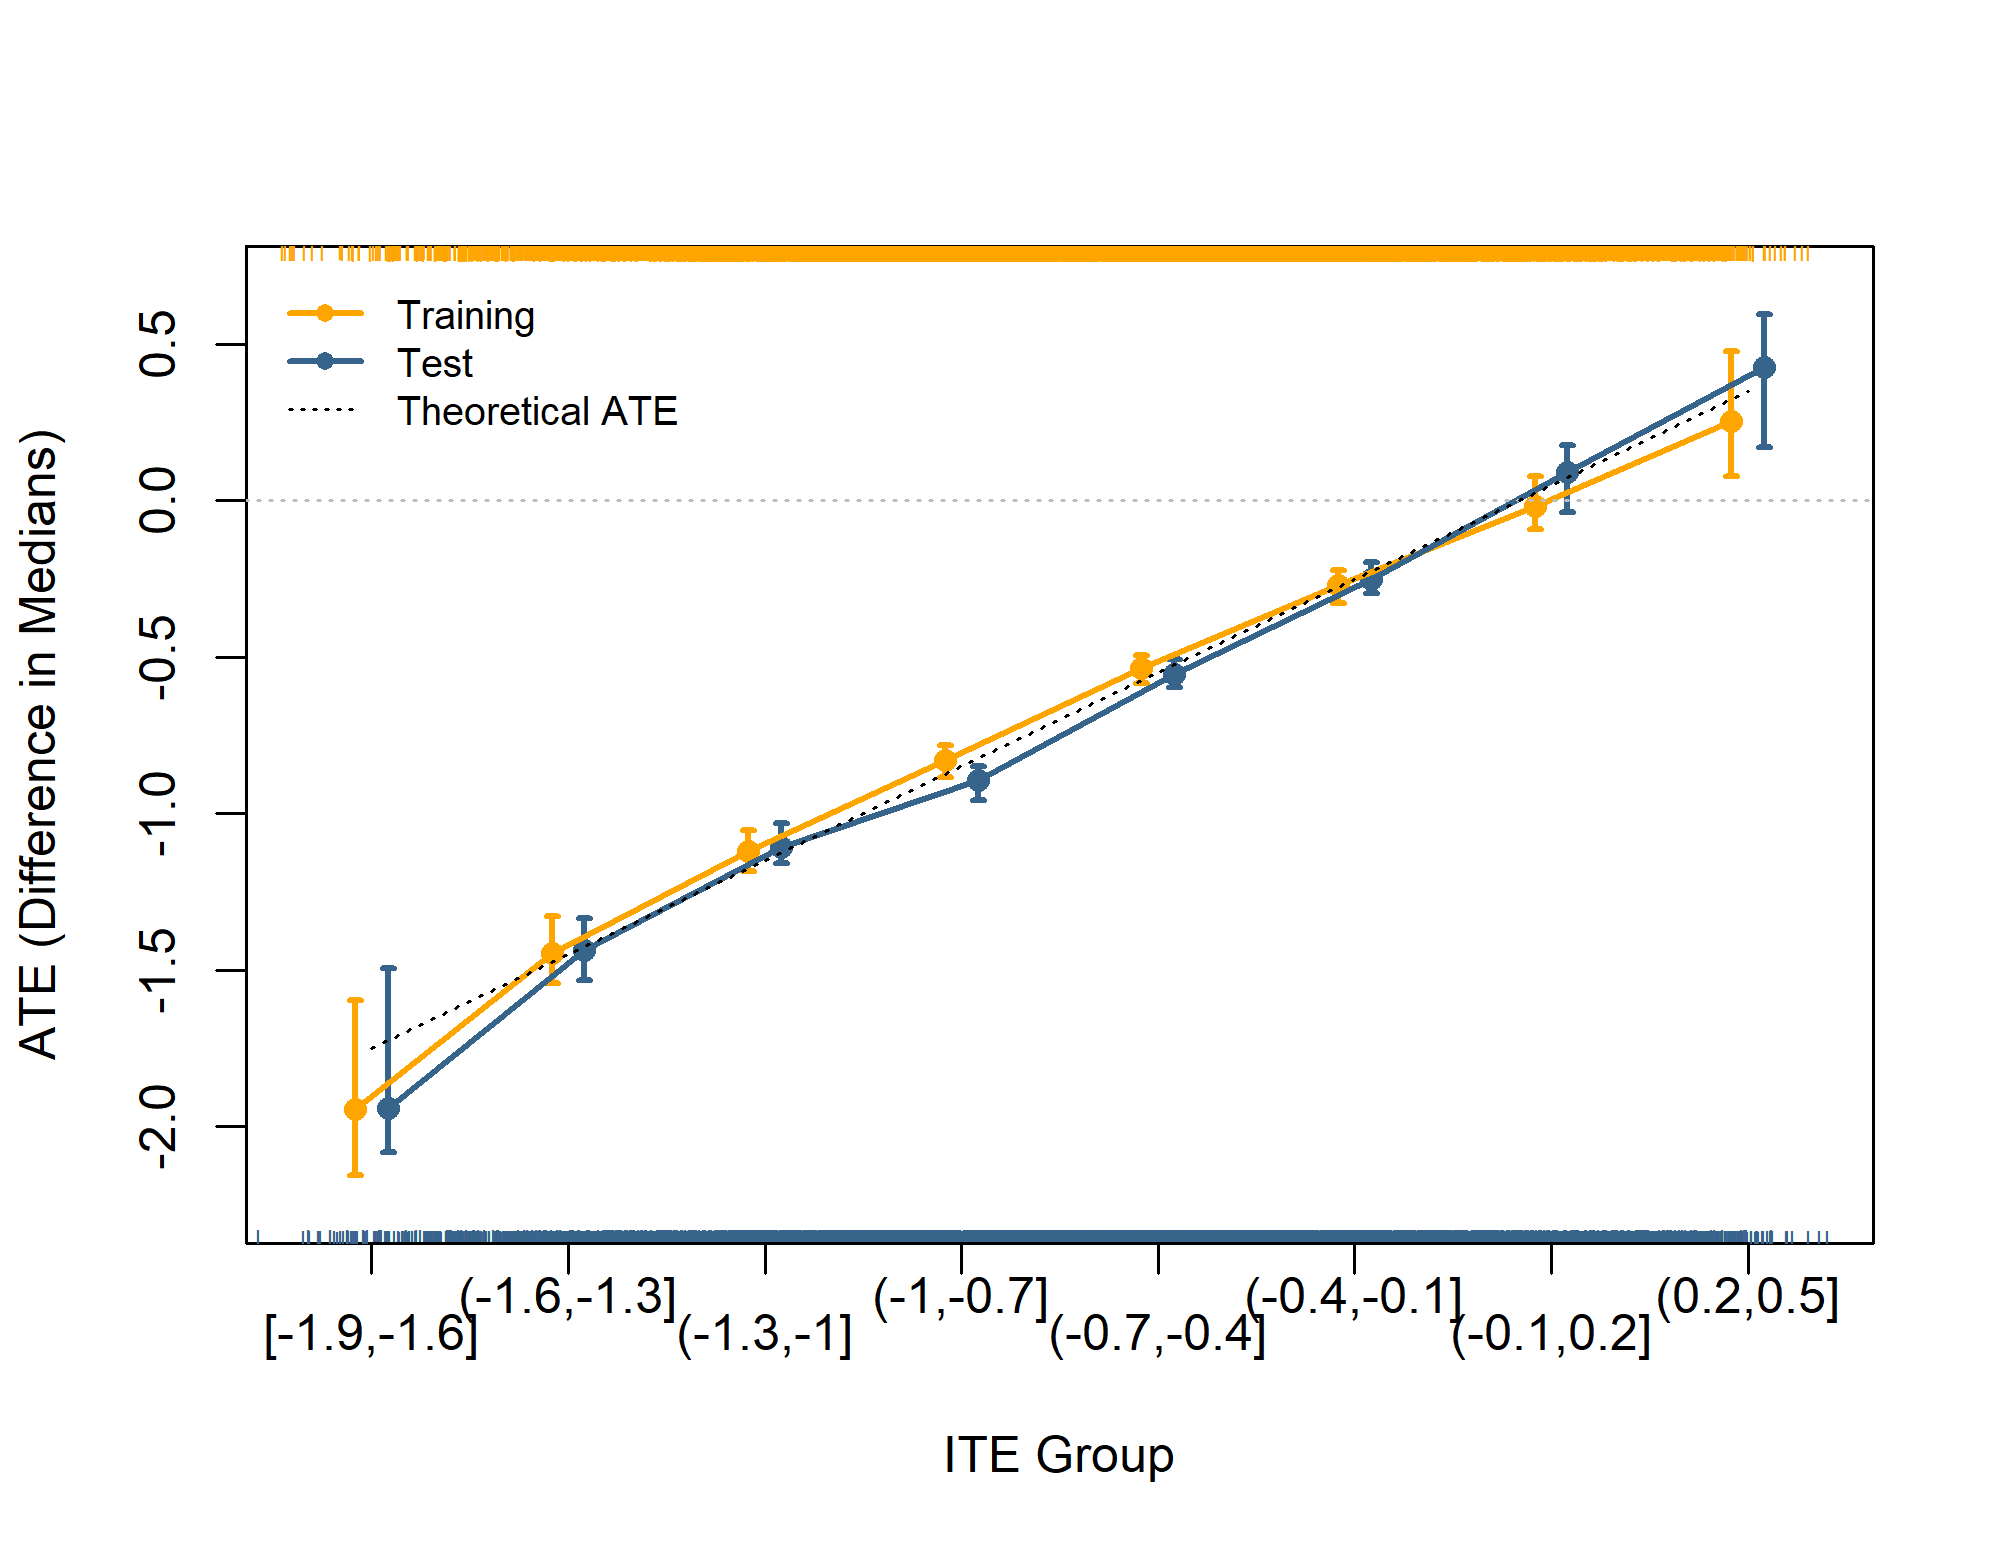
\includegraphics[width=0.8\textwidth]{img/results/rct_scenario1_ITE_ATE.png}
\vspace{-15pt}
\caption{ITE-ATE plot for Scenario (1) in the RCT setting, which includes direct and interaction effects. Individuals are grouped into bins based on their estimated ITEs, and within each bin, the ATE is calculated as the difference in medians of the observed outcomes under the two treatments. 95\% bootstrap confidence intervals indicate the uncertainty.}
\label{fig:rct_scenario1_ite_ATE}
\end{figure}


% start a new page
\clearpage


\subsection{Scenario (2): With direct effect, but no interaction effects}

\begin{figure}[H]
\centering
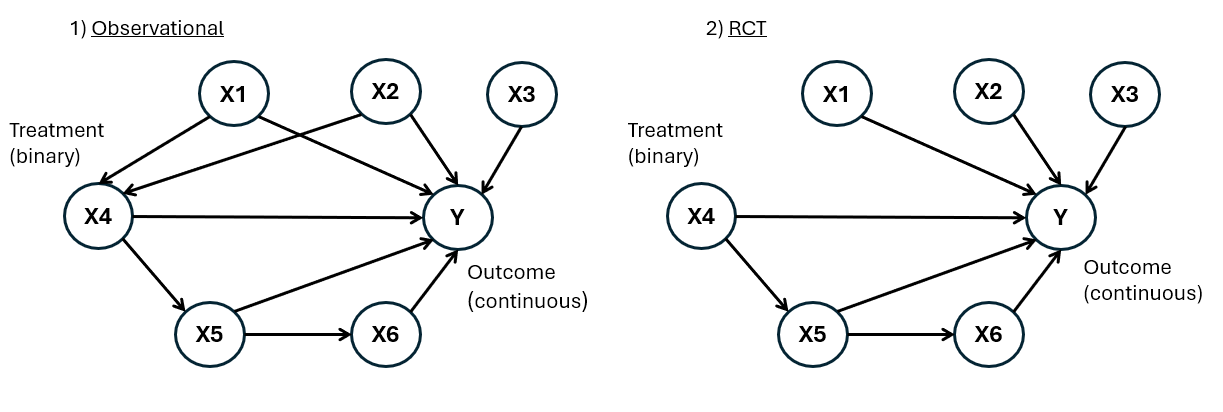
\includegraphics[width=0.85\textwidth]{img/exp4_dag_2.png}
\caption{DAGs for Scenario~(2), which includes a direct effect of the treatment on the outcome, but no interaction effects that would induce treatment effect heterogeneity. Left: Observational setting; Right: RCT setting.}
\label{fig:ite_dag_observational_2}
\end{figure}

Scenario (2) includes a direct effect of the treatment on the outcome, while the coefficients for the interaction terms are set to zero. This results in less heterogeneity in the ITE distribution compared to Scenario (1), as shown in Figure~\ref{fig:scenario2_ite_distribution_dgp}. Why there is still some heterogeneity despite the absence of interactions is discussed in Section~\ref{sec:disc_experiment4}. The observational and interventional densities generated by the fitted TRAM-DAG closely match the true densities defined by the DGP, as illustrated in Figures~\ref{fig:scenario2_sampling_distributions_vertical} and~\ref{fig:scenario2_outcome_distributions}. However, there is a notable difference in variance between the estimated and true ITE distributions, visible in Figures~\ref{fig:scenario2_ite_densities_train_test} and~\ref{fig:scenario2_ite_scatter_train_test}. The ITE-ATE plots in Figures~\ref{fig:observ_scenario2_ite_ATE} and \ref{fig:rct_scenario2_ite_ATE} are less informative than in Scenario (1), as expected given the reduced heterogeneity. Table~\ref{tab:scenario2_ate_comparison} presents the ATE measures for Scenario (2). In the test set of the RCT setting, the ATE based on the true ITEs was -0.633, while the ATE based on the estimated ITEs was -0.586.


\begin{table}[htbp]
\centering
\small
\caption{Scenario (2), including a direct treatment effect but no interaction effects: Comparison of ATE measures across train and test sets for the observational and RCT setting. $\text{Y}_\text{observed}^{(\text{Tr})}$ denotes the observed outcome under the treatment ($\text{Tr}$) actually received. The estimated ATE from $\text{mean}(\text{ITE}_\text{estimated})$ can be directly compared to the true $\text{mean}(\text{ITE}_\text{true})$, whereas comparisons to the empirical ATEs based on outcome differences should be interpreted with caution.}
\label{tab:scenario2_ate_comparison}
\begin{tabular}{l c c c c}
\toprule
\textbf{Measure} & \multicolumn{2}{c}{\textbf{Observational}} & \multicolumn{2}{c}{\textbf{RCT}} \\
\cmidrule(lr){2-3} \cmidrule(lr){4-5}
 & \textbf{Train} & \textbf{Test} & \textbf{Train} & \textbf{Test} \\
\midrule
ATE as $\text{mean}(\text{Y}_\text{observed}^{(1)}) - \text{mean}(\text{Y}_\text{observed}^{(0)})$ 
& NA & NA 
& -0.569 
& -0.572 \\

ATE as $\text{median}(\text{Y}_\text{observed}^{(1)}) - \text{median}(\text{Y}_\text{observed}^{(0)})$  
& NA & NA 
& -0.629 
& -0.639 \\

ATE as mean(ITE$_\text{true}$)  
& -0.633 
& -0.633 
& -0.633 
& -0.633 \\

ATE as mean(ITE$_\text{estimated}$) 
& -0.645 
& -0.644 
& -0.587 
& -0.586 \\
\bottomrule
\end{tabular}
\end{table}

% 
% \begin{table}[htbp]
% \centering
% \small
% \caption{Scenario (2), including a direct treatment but no interaction effects: Comparison of ATE measures across train and test sets for the observational and RCT setting.}
% \label{tab:scenario2_ate_comparison_old}
% \begin{tabular}{l c c c c}
% \toprule
% \textbf{Measure} & \multicolumn{2}{c}{\textbf{Observational}} & \multicolumn{2}{c}{\textbf{RCT}} \\
% \cmidrule(lr){2-3} \cmidrule(lr){4-5}
%  & \textbf{Train} & \textbf{Test} & \textbf{Train} & \textbf{Test} \\
% \midrule
% ATE as $\text{mean}(\text{Y}_\text{observed}^{(1)}) - \text{mean}(\text{Y}_\text{observed}^{(0)})$ & NA & NA & round(rct_scenario2$dev_ATE_observed_Y_mean_diff, 3) & round(rct_scenario2$val_ATE_observed_Y_mean_diff, 3) \\
% ATE as $\text{median}(\text{Y}_\text{observed}^{(1)}) - \text{median}(\text{Y}_\text{observed}^{(0)})$  & NA & NA & round(rct_scenario2$dev_ATE_observed_Y_median_diff, 3) & round(rct_scenario2$val_ATE_observed_Y_median_diff, 3) \\
% ATE as mean(ITE$_\text{true}$)  & round(observ_scenario2$dev_ITE_median_average, 3) & round(observ_scenario2$val_ITE_median_average, 3) & round(rct_scenario2$dev_ITE_median_average, 3) & round(rct_scenario2$val_ITE_median_average, 3) \\
% ATE as mean(ITE$_\text{estimated}$) & round(observ_scenario2$dev_ITE_median_pred_average, 3) & round(observ_scenario2$val_ITE_median_pred_average, 3) & round(rct_scenario2$dev_ITE_median_pred_average, 3) & round(rct_scenario2$val_ITE_median_pred_average, 3) \\
% \bottomrule
% \end{tabular}
% \end{table}



\begin{figure}[htbp]
\centering
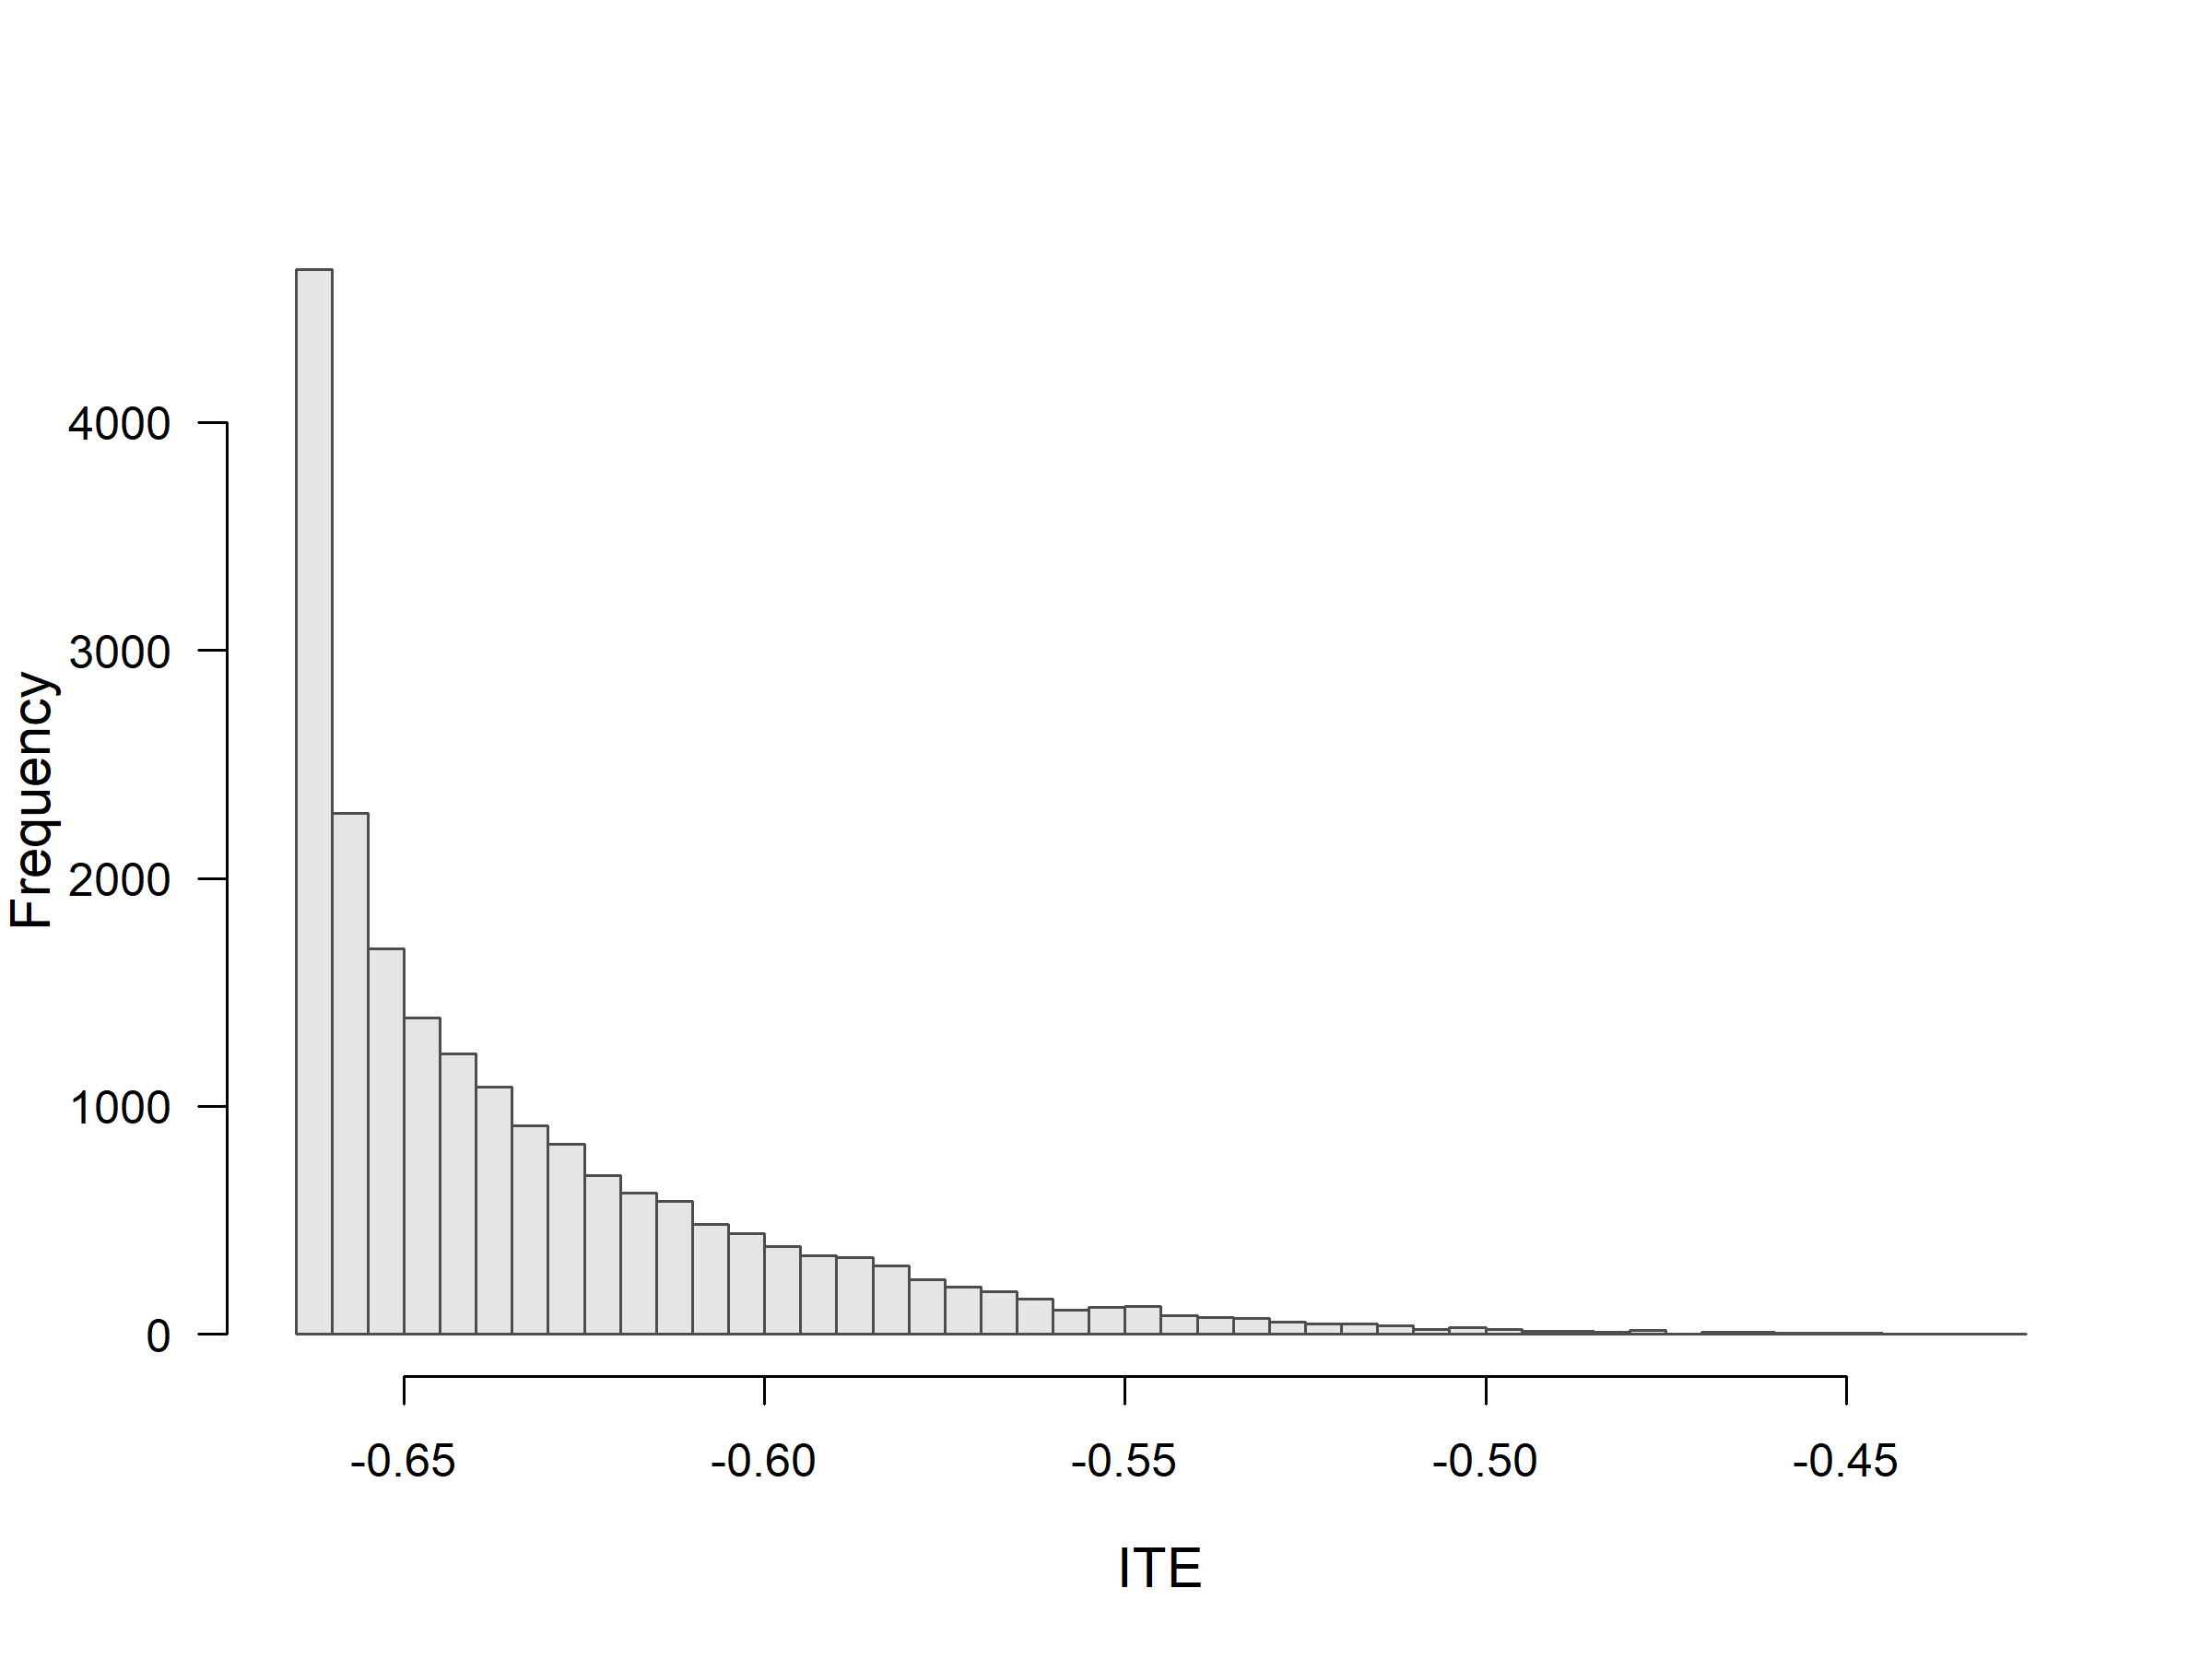
\includegraphics[width=0.7\textwidth]{img/results/observ_scenario2_ite_distribution_dgp.png}
\caption{True ITE distribution resulting from the DGP for Scenario~(2), which includes a direct treatment effect but no interaction effects. The true ITEs are identical in the observational and RCT settings, as they depend only on the potential outcomes under both treatment allocations.}
\label{fig:scenario2_ite_distribution_dgp}
\end{figure}



\begin{figure}[htbp]
\centering
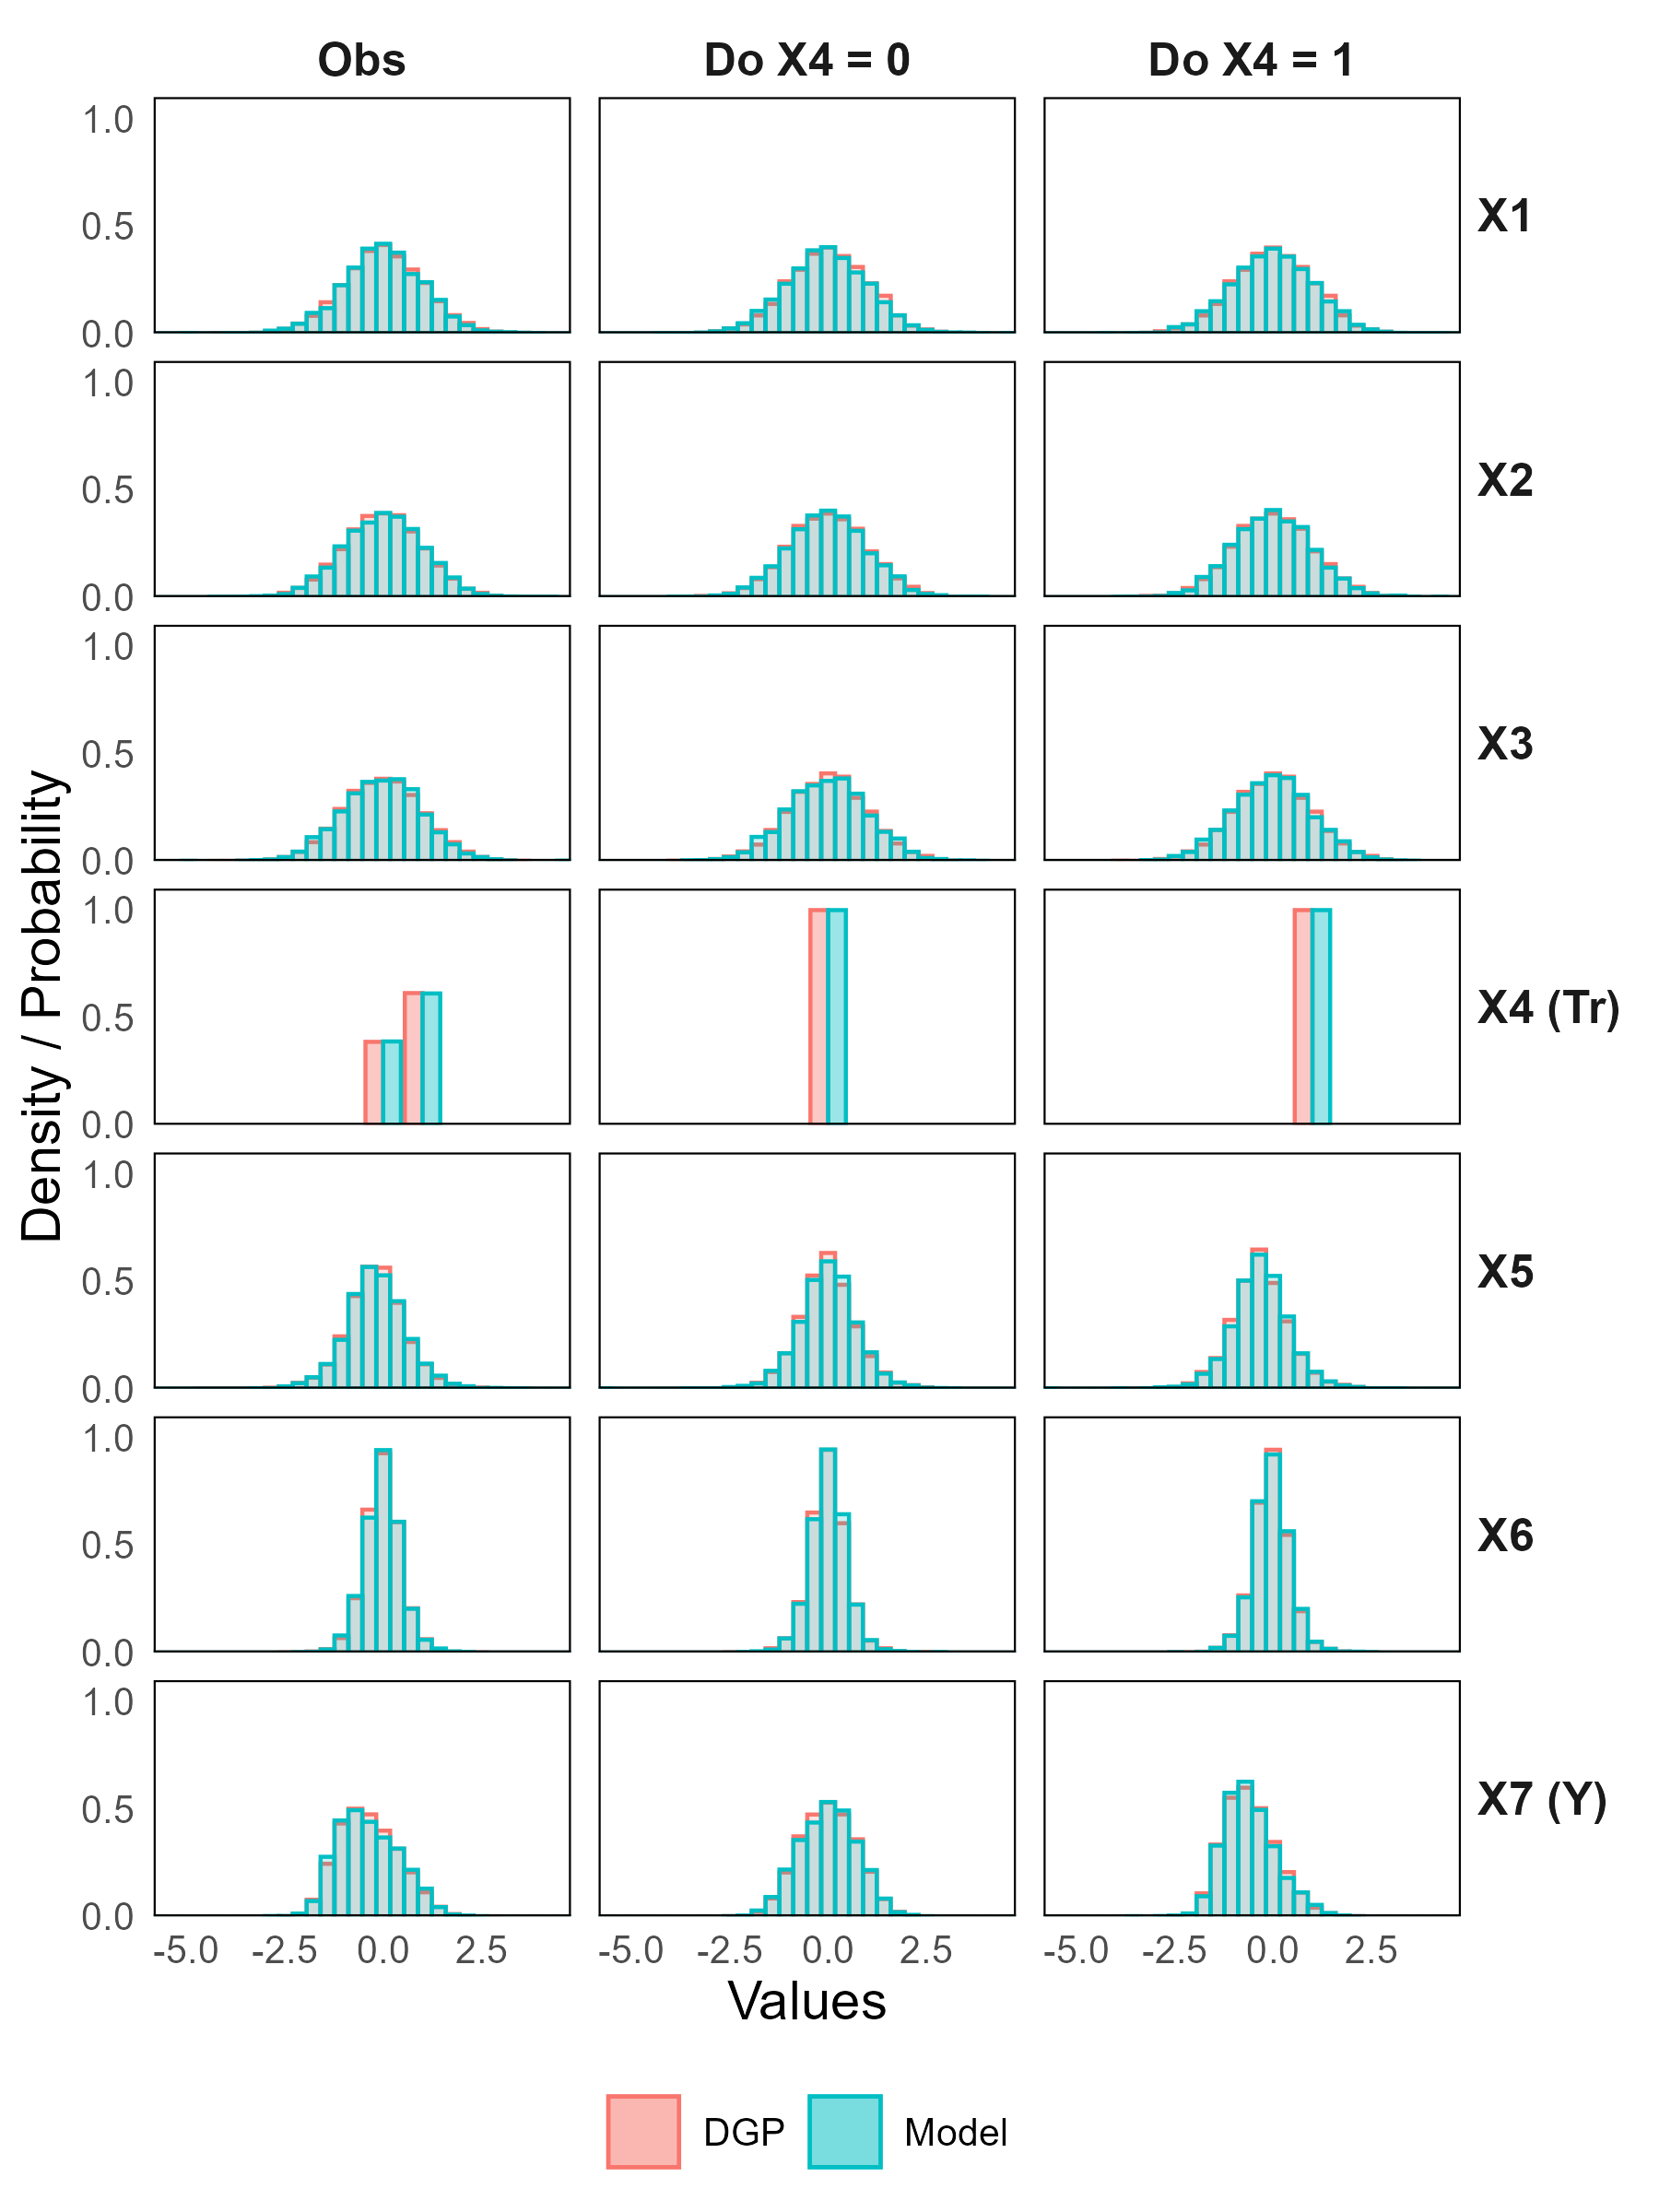
\includegraphics[width=0.45\textwidth]{img/results/observ_scenario2_sampling_distributions_vertical.png}
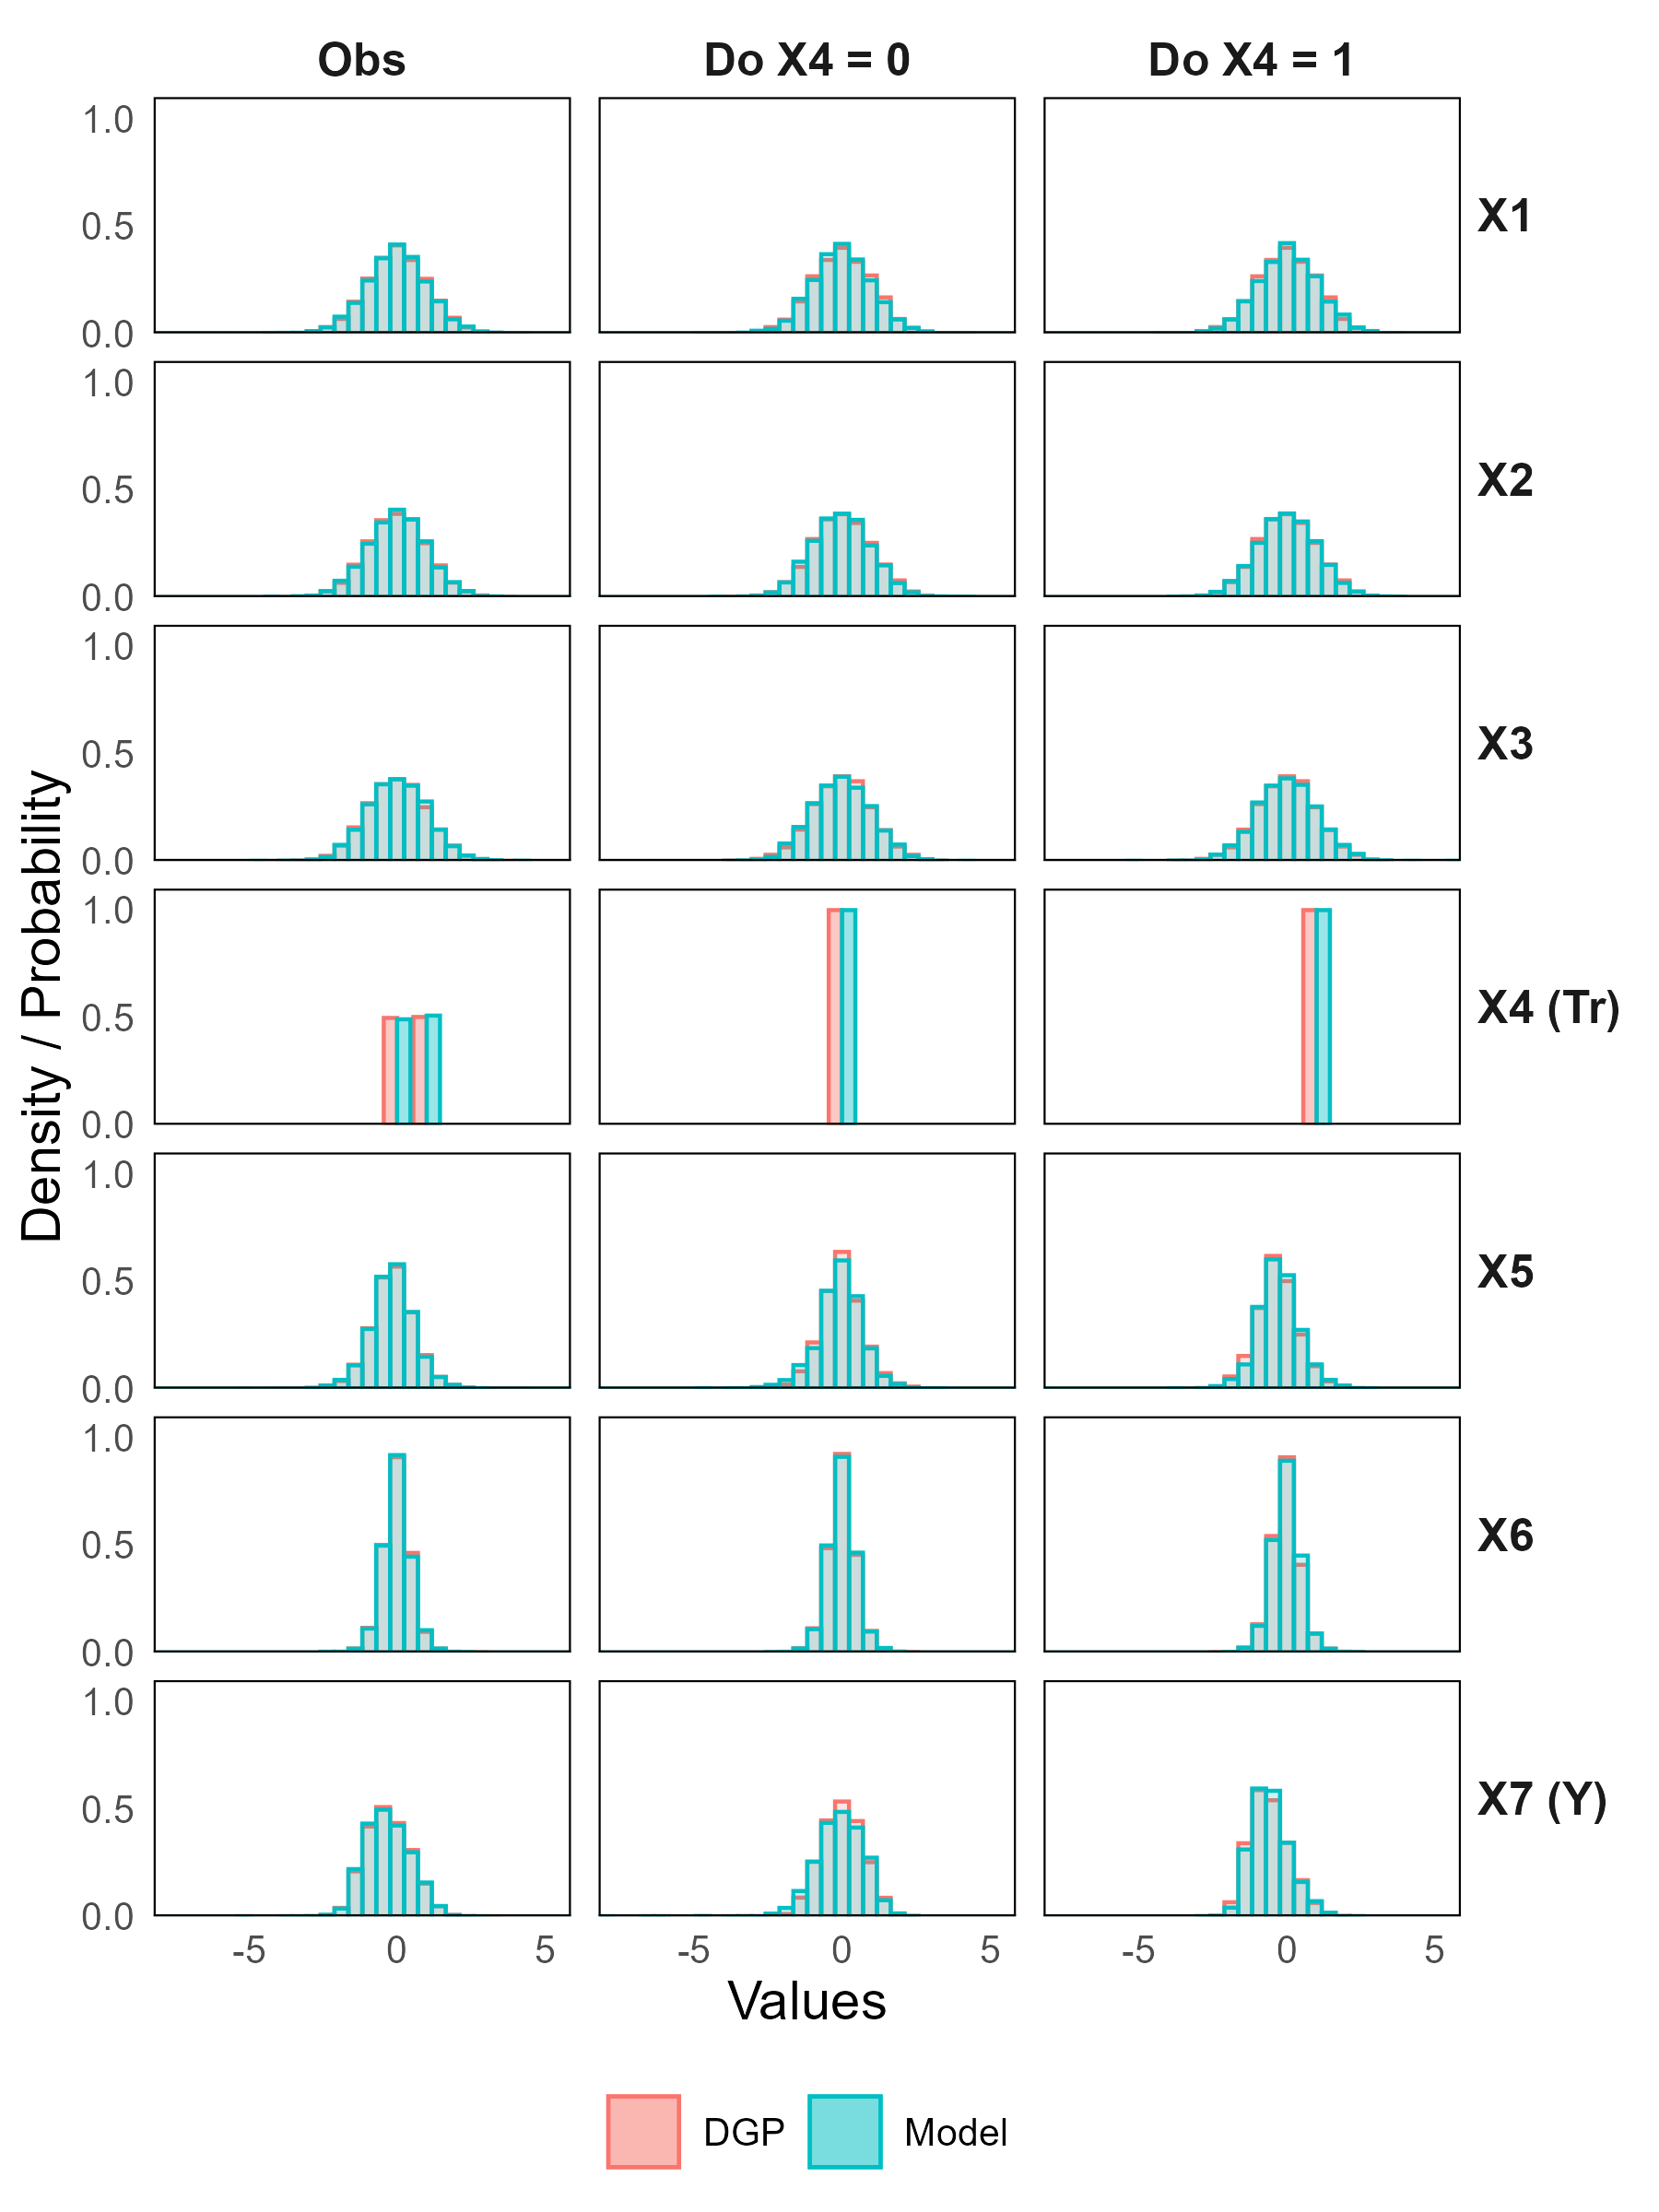
\includegraphics[width=0.45\textwidth]{img/results/rct_scenario2_sampling_distributions_vertical.png}
\caption{Marginal distributions of variables from the DGP and samples generated by the fitted TRAM-DAG for Scenario~(2), which includes a direct treatment effect but no interaction effects. The distributions are shown as observed (Obs), under control intervention (do($X_4 = 0$)), and under treatment intervention (do($X_4 = 1$)). Left: Observational; Right: RCT setting.}
\label{fig:scenario2_sampling_distributions_vertical}
\end{figure}


\begin{figure}[htbp]
\centering
\includegraphics[width=0.45\textwidth]{img/results/observ_scenario2_X7_treatment_densities.png}
\includegraphics[width=0.45\textwidth]{img/results/rct_scenario2_X7_treatment_densities.png}
\caption{Distributions of the outcome variable ($X_7$) under treatment and control interventions for Scenario~(2), which includes a direct treatment effect but no interaction effects. This plot provides a higher-resolution view of the $X_7$ panels under do($X_4 = 0$) and do($X_4 = 1$) from Figure~\ref{fig:scenario2_sampling_distributions_vertical}. Left: Observational; Right: RCT setting.}
\label{fig:scenario2_outcome_distributions}
\end{figure}






\begin{figure}[htbp]
\centering
\includegraphics[width=0.33\textwidth]{img/results/observ_scenario2_ITE_densities_train_test.png}
\includegraphics[width=0.33\textwidth]{img/results/rct_scenario2_ITE_densities_train_test.png}
\vspace{-17pt}
\caption{Densities of estimated ITEs compared to the true ITEs in the training and test datasets for Scenario~(2), which includes a direct treatment effect but no interaction effects. Left: Observational; Right: RCT setting.}
\label{fig:scenario2_ite_densities_train_test}
\end{figure}






\begin{figure}[htbp]
\centering
\includegraphics[width=0.33\textwidth]{img/results/observ_scenario2_ITE_scatter_train_test.png}
\includegraphics[width=0.33\textwidth]{img/results/rct_scenario2_ITE_scatter_train_test.png}
\vspace{-17pt}
\caption{Scatterplots of estimated ITEs compared to the true ITEs in the training and test datasets for Scenario~(2), which includes a direct treatment effect but no interaction effects. Left: Observational; Right: RCT setting.}
\label{fig:scenario2_ite_scatter_train_test}
\end{figure}




\begin{figure}[htbp]
\centering
\includegraphics[width=0.8\textwidth]{img/results/observ_scenario2_ITE_ATE.png}
\vspace{-15pt}
\caption{ITE-ATE plot for Scenario~(2) in the observational setting, which includes a direct treatment effect but no interaction effects. Individuals are grouped into bins based on their estimated ITEs, and in each bin, the ATE is computed as the difference in medians of the observed outcomes under treatment and control. The 95\% bootstrap confidence intervals indicate uncertainty.}
\label{fig:observ_scenario2_ite_ATE}
\end{figure}



\begin{figure}[htbp]
\centering
\includegraphics[width=0.8\textwidth]{img/results/rct_scenario2_ITE_ATE.png}
\vspace{-15pt}
\caption{ITE-ATE plot for Scenario~(2) in the RCT setting, which includes a direct treatment effect but no interaction effects. Individuals are grouped into bins based on their estimated ITEs, and in each bin, the ATE is computed as the difference in medians of the observed outcomes under treatment and control. The 95\% bootstrap confidence intervals indicate uncertainty.}
\label{fig:rct_scenario2_ite_ATE}
\end{figure}



\clearpage 



\subsection{Scenario (3): No direct effect, but with interaction effects}

\begin{figure}[H]
\centering
\includegraphics[width=0.85\textwidth]{img/exp4_dag_3.png}
\caption{DAGs for Scenario~(3), which includes no direct effect of the treatment on the outcome, but interaction effects with covariates $X_2$ and $X_3$. Left: Observational setting; Right: RCT setting.}
\label{fig:ite_dag_observational_3}
\end{figure}

Scenario~(3) includes no direct effect of the treatment on the outcome, but does include interaction effects between the treatment and covariates $X_2$ and $X_3$. Compared to Scenario~(1), removing the direct effect results in a more centered ITE distribution, as shown in Figure~\ref{fig:scenario3_ite_distribution_dgp}. In the test set of the RCT setting, the ATE measured as the difference in means was -0.048, with a 95\% confidence interval from -0.068 to -0.028.




\begin{table}[htbp]
\centering
\small
\caption{Scenario (3), without a direct treatment effect but including interaction effects: Comparison of ATE measures across train and test sets for the observational and RCT setting. $\text{Y}_\text{observed}^{(\text{Tr})}$ denotes the observed outcome under the treatment ($\text{Tr}$) actually received. The estimated ATE from $\text{mean}(\text{ITE}_\text{estimated})$ can be directly compared to the true $\text{mean}(\text{ITE}_\text{true})$, whereas comparisons to the empirical ATEs based on outcome differences should be interpreted with caution.}
\label{tab:scenario3_ate_comparison}
\begin{tabular}{l c c c c}
\toprule
\textbf{Measure} & \multicolumn{2}{c}{\textbf{Observational}} & \multicolumn{2}{c}{\textbf{RCT}} \\
\cmidrule(lr){2-3} \cmidrule(lr){4-5}
 & \textbf{Train} & \textbf{Test} & \textbf{Train} & \textbf{Test} \\
\midrule
ATE as $\text{mean}(\text{Y}_\text{observed}^{(1)}) - \text{mean}(\text{Y}_\text{observed}^{(0)})$ 
& NA & NA 
& -0.048 
& -0.048 \\

ATE as $\text{median}(\text{Y}_\text{observed}^{(1)}) - \text{median}(\text{Y}_\text{observed}^{(0)})$  
& NA & NA 
& -0.048 
& -0.059 \\

ATE as mean(ITE$_\text{true}$)  
& -0.065 
& -0.068 
& -0.065 
& -0.068 \\

ATE as mean(ITE$_\text{estimated}$) 
& -0.059 
& -0.061 
& -0.051 
& -0.053 \\
\bottomrule
\end{tabular}
\end{table}


% \begin{table}[htbp]
% \centering
% \small
% \caption{Scenario (3), without direct treatment effect but including interaction effects: Comparison of ATE measures across train and test sets for the observational and RCT setting.}
% \label{tab:scenario3_ate_comparison_old}
% \begin{tabular}{l c c c c}
% \toprule
% \textbf{Measure} & \multicolumn{2}{c}{\textbf{Observational}} & \multicolumn{2}{c}{\textbf{RCT}} \\
% \cmidrule(lr){2-3} \cmidrule(lr){4-5}
%  & \textbf{Train} & \textbf{Test} & \textbf{Train} & \textbf{Test} \\
% \midrule
% ATE as $\text{mean}(\text{Y}_\text{observed}^{(1)}) - \text{mean}(\text{Y}_\text{observed}^{(0)})$ & NA & NA & round(rct_scenario3$dev_ATE_observed_Y_mean_diff, 3) & round(rct_scenario3$val_ATE_observed_Y_mean_diff, 3) \\
% ATE as $\text{median}(\text{Y}_\text{observed}^{(1)}) - \text{median}(\text{Y}_\text{observed}^{(0)})$ & NA & NA & round(rct_scenario3$dev_ATE_observed_Y_median_diff, 3) & round(rct_scenario3$val_ATE_observed_Y_median_diff, 3) \\
% ATE as mean(ITE$_\text{true}$)  & round(observ_scenario3$dev_ITE_median_average, 3) & round(observ_scenario3$val_ITE_median_average, 3) & round(rct_scenario3$dev_ITE_median_average, 3) & round(rct_scenario3$val_ITE_median_average, 3) \\
% ATE as mean(ITE$_\text{estimated}$) & round(observ_scenario3$dev_ITE_median_pred_average, 3) & round(observ_scenario3$val_ITE_median_pred_average, 3) & round(rct_scenario3$dev_ITE_median_pred_average, 3) & round(rct_scenario3$val_ITE_median_pred_average, 3) \\
% \bottomrule
% \end{tabular}
% \end{table}
% 


\begin{figure}[htbp]
\centering
\includegraphics[width=0.7\textwidth]{img/results/observ_scenario3_ite_distribution_dgp.png}
\caption{True ITE distribution resulting from the DGP for Scenario~(3), which includes interaction effects but no direct treatment effect. The true ITEs are identical in the observational and RCT settings, since they are based on the potential outcomes under both treatment allocations. Left: Observational; Right: RCT setting.}
\label{fig:scenario3_ite_distribution_dgp}
\end{figure}



\begin{figure}[htbp]
\centering
\includegraphics[width=0.45\textwidth]{img/results/observ_scenario3_sampling_distributions_vertical.png}
\includegraphics[width=0.45\textwidth]{img/results/rct_scenario3_sampling_distributions_vertical.png}
\caption{Marginal distributions of DGP variables and samples generated by the fitted TRAM-DAG for Scenario~(3), which includes interaction effects but no direct treatment effect. The distributions are shown as observed (Obs), under control intervention (do($X_4 = 0$)), and under treatment intervention (do($X_4 = 1$)). Left: Observational; Right: RCT setting.}
\label{fig:scenario3_sampling_distributions_vertical}
\end{figure}

\begin{figure}[htbp]
\centering
\includegraphics[width=0.45\textwidth]{img/results/observ_scenario3_X7_treatment_densities.png}
\includegraphics[width=0.45\textwidth]{img/results/rct_scenario3_X7_treatment_densities.png}
\caption{Distributions of the outcome variable ($X_7$) under treatment and control interventions for Scenario~(3), which includes interaction effects but no direct treatment effect. This plot provides a higher resolution view of the $X_7$ panels under do($X_4 = 0$) and do($X_4 = 1$) from Figure~\ref{fig:scenario3_sampling_distributions_vertical}. Left: Observational; Right: RCT setting.}
\label{fig:scenario3_outcome_distributions}
\end{figure}




\begin{figure}[htbp]
\centering
\includegraphics[width=0.33\textwidth]{img/results/observ_scenario3_ITE_densities_train_test.png}
\includegraphics[width=0.33\textwidth]{img/results/rct_scenario3_ITE_densities_train_test.png}
\vspace{-17pt}
\caption{Densities of estimated ITEs compared to the true ITEs in the training and test datasets for Scenario~(3), which includes interaction effects but no direct treatment effect. Left: Observational; Right: RCT setting.}
\label{fig:scenario3_ite_densities_train_test}
\end{figure}






\begin{figure}[htbp]
\centering
\includegraphics[width=0.33\textwidth]{img/results/observ_scenario3_ITE_scatter_train_test.png}
\includegraphics[width=0.33\textwidth]{img/results/rct_scenario3_ITE_scatter_train_test.png}
\vspace{-17pt}
\caption{Scatterplots of estimated ITEs compared to the true ITEs in the training and test datasets for Scenario~(3), which includes interaction effects but no direct treatment effect. Left: Observational; Right: RCT setting.}
\label{fig:scenario3_ite_scatter_train_test}
\end{figure}




\begin{figure}[htbp]
\centering
\includegraphics[width=0.8\textwidth]{img/results/observ_scenario3_ITE_ATE.png}
\vspace{-15pt}
\caption{ITE-ATE plot for Scenario~(3) in the observational setting, which includes interaction effects but no direct treatment effect. Individuals are grouped into bins based on the estimated ITE, and within each bin the ATE is computed as the difference in medians of the observed outcomes under treatment and control. 95\% bootstrap confidence intervals reflect the uncertainty.}
\label{fig:observ_scenario3_ite_ATE}
\end{figure}


\begin{figure}[htbp]
\centering
\includegraphics[width=0.8\textwidth]{img/results/rct_scenario3_ITE_ATE.png}
\vspace{-15pt}
\caption{ITE-ATE plot for Scenario~(3) in the RCT setting, which includes interaction effects but no direct treatment effect. Individuals are grouped into bins based on the estimated ITE, and within each bin the ATE is computed as the difference in medians of the observed outcomes under treatment and control. 95\% bootstrap confidence intervals reflect the uncertainty.}
\label{fig:rct_scenario3_ite_ATE}
\end{figure}







%  --> the following will be used in Experiment 4 (methods)
% http://www.mit.edu/~vchern/papers/ch_iqr_ema.pdf estimate the quantile treatment effect (heterogeneous) with instrumental variables, it looks very similar to the TRAM-DAG approach: *This interpretation makes quantile analysis an interesting tool for describing and learning the structure of heterogeneous treatment effects and controlling for unobserved heterogeneity."

% https://www.rfberlin.com/wp-content/uploads/2024/12/24030.pdf good book/paper about instrumental variables, also talks about potential outcomes (but i should maybe not go too much into detial)

% - maybe include somewhere the discussion about the difference between discrimination and claibraion:
% https://bavodc.github.io/websiteCalibrationCurves/articles/CalibrationCurves.html




% An example could be the psychological condition of a patient which might also affect how the treatment works, this is not a confounder but an effect modifier, and i would assume that this variable is rarely recorede or measured.



% enforce that starts after all floats have been displayed
\FloatBarrier


\section{Discussion} \label{sec:disc_experiment4}


We analyzed ITE estimation under an observational setting (confounded) and under an RCT setting (randomized treatment allocation) in three different scenarios: direct and interaction treatment effect, only direct but no interaction effect, and no direct but with interaction effect. The TRAM-DAG could successfully estimate the ITE in Scenario 1 and Scenario 3 where interaction effects were present. There was no notable difference between the observational and RCT settings. Scatterplots of estimated ITEs vs. true ITEs showed good prediction accuracy (see Figures \ref{fig:scenario1_ite_scatter_train_test} and \ref{fig:scenario3_ite_scatter_train_test}). Also the ATE based on the mean of estimated ITEs was close to the ATE based on true ITEs in both scenarios (see Tables \ref{tab:scenario1_ate_comparison} and \ref{tab:scenario3_ate_comparison}). These results highlight TRAM-DAG's ability to compute counterfactuals for mediators and to estimate individualized treatment effects even in relatively complex DAG structures.



In Scenario 2, where no interaction effects were present, ITE estimation was poor. This aligns with our discovery in Experiment 3 that when true heterogeneity is weak, models tended to estimate too large heterogeneity, as e.g. shown in Figure \ref{fig:small_interaction_tuned_rf_tlearner} with the T-learner tuned random forest.

\medskip

What might be surprising in Scenario 2 is the presence of heterogeneity (true ITEs), despite the absence of explicitly specified interaction terms in the data-generating process. As shown in Figure~\ref{fig:scenario2_ite_distribution_dgp}, one might have expected the ITEs to be constant across individuals -- equal to the ATE -- given the model's additivity on the log-odds scale. However, as described by \citet{hoogland2021}, such heterogeneity arises because a constant treatment effect on the log-odds scale does not translate into a constant effect on a different scale, such as the probability scale. This phenomenon results from the nonlinearity of the inverse-link function (e.g., $\text{logit}^{-1}$), which transforms additive effects in the linear predictor into non-additive effects on the outcome scale. As the authors point out, the same shift induced by the treatment on the log-odds scale leads to different absolute risk reductions depending on the outcome risk under the control treatment. In other words, even with a homogeneous effect on the linear predictor, variation in covariates $\mathbf{X}$ leads to different treatment effects on the probability scale.

This would not have occurred under a linear model where the transformation function $h$ is the identity. In that case, the ITE would simplify as follows:

\begin{equation}
\text{ITE} = \mathbb{E}[Y(1)] - \mathbb{E}[Y(0)] = (\beta_0 + \beta_t + \boldsymbol{\beta}_x^\top \mathbf{X} + \epsilon) - (\beta_0 + \boldsymbol{\beta}_x^\top \mathbf{X} + \epsilon) = \beta_t
\end{equation}

Here, the ITE is constant and equal to the treatment coefficient, independent of the covariates or the noise term, which cancels out.

In contrast, under a nonlinear model, such as the logistic transformation model with a nonlinear intercept function used in this experiment, the ITE becomes:

\begin{equation}
\text{ITE} = \mathbb{E}[h^{-1}(Z + \beta_t + \boldsymbol{\beta}_x^\top \mathbf{X})] - \mathbb{E}[h^{-1}(Z + \boldsymbol{\beta}_x^\top \mathbf{X})]
\end{equation}

Since $h^{-1}$ is nonlinear, the difference depends on the covariate profile $\mathbf{X}$ and on the noise term $Z$, even though the treatment effect $\beta_t$ is additive in the linear predictor, i.e., on the log-odds scale. It may therefore be worth thinking about whether analyzing the ITE on a scale where the effect is constant offers any advantages.

\medskip


Maybe also related to this phenomenon, although not directly in the context of ITEs, is the concept of noncollapsibility, as discussed by \citet{dandl2025}. Noncollapsibility refers to the case when the treatment effect estimated from a marginal model (i.e., without covariates) does not correspond to the marginal effect that is obtained by averaging conditional treatment effects (i.e., adjusted for prognostic covariates) over the covariate distribution \citet{aalen2015}. Hence, treatment effects from two conditional models that use different sets of covariates for adjustment are not directly comparable if the model is noncollapsible. \citet{dandl2025} proposed a solution based on nonparanormal models \citep{liu2009, klein2022} to estimate a marginal treatment effect, while maintaining comparability (unaffected by covariates) and gaining from increased precision by adjusting for prognostic factors. Whether and how such an approach could be applied to ITE estimation is not explored further in this thesis.


% Maybe also related to this phenomenon, although not in the context of ITEs, might be the concept of non-collapsibility, as discussed by \citet{dandl2025}. Non-collapsibility refers to the case when the treatment effect from a marginal model does not correspond to the marginal effect that is obtained from a conditional treatment effect (i.e. adjusted for prognostic covariates) by averaging over the prognostic variables. Hence, treatment effects from two conditional models that used different sets of covariate for adjustments are not comparable if a model is non-collapsible. The authors proposed a solution based on nonparanomrmal models (\citealp{{liu2009}; \citealp{klein2022}) to estimate a marginal treatment effect, while maintaining comparability (unaffected by covariates) and gaining from increased precision by adjusting for prognostic factors. However, if and how this would translate to ITE estimation goes beyond the scope of this thesis.

% What might be surprising is that in Scenario 2 where we dont have explicitly included interaction terms in the data generating process, there is still some heterogeneity in the treatment effect, as shown in Figure \ref{fig:scenario2_ite_distribution_dgp}. One might expect that the ITE is constant across all individuals in such a case, and equal to the ATE. 
% 
% \citep{hoogland2021} chapter 4.1 well described this phenomenon of non-additivity leaving the log-odds scale.
% % the problem with non-additivity is perffectly described in Hoogland "A tutorial on individualized treatment effect prediction from randomized trials with a binary endpoint
% 
% However since we used a non linear transformatino function as intercept in the data generating process (as would likely be the case in a real world setting), the treatment effect is not constant across all individuals (which should correspond to the ATE). When a linear transformation function would be applied (as for example a linear regression is specified, where the latent noise distribution would be the standard normal and the transformation function would be linear) then the noise term cancels out when calculating the ITE, leading to a constant ITE when no interactions are present: $\text{ITE} = \text{E}[Y(1)] -\text{E}[Y(0)] = (\beta_0 + \beta_t 1 + \beta_x X + \epsilon) - (\beta_0 + \beta_t 0 + \beta_x X + \epsilon) = \beta_t$.
% 
% In a model with nonlinear transformation, as in this experiment, the noise term does not cancel out anymore leading to different ITEs for patients with different characteristics.
% 
% \begin{equation}
% \text{ITE} = \text{E}[Y(1) - Y(0)] = \text{E}[h^{-1}(Z + \beta_t 1 + \beta_x X)] - \text{E}[h^{-1}(Z + \beta_t 0 + \beta_x X)] 
% \end{equation}
% 
% where $h$ is the nonlinear transformation function, $Z$ is the latent noise term, $\beta_t$ is the direct treatment effect and $\beta_x$ are the coefficients of the covariates. The state of the covariates $X$ alters the position on the transformation function and thereby affects the difference between the two terms. If the transformation was fixed to be linear, the difference would be constant independent of the state of the covariates $X$. 

% (This also has to do with non-collapsibility as discussed by susanne and torsten , also check Beates Mail 21.06.2025, and chatgpt discussion)



% cite susanne and torsten paper: https://arxiv.org/abs/2503.01657






%%%%%%%%%%%%%%%%%%%%%%%%%%%%%%%%%%%%%%%%%%%%%%%%%%%%%%%%%%%%%%%%%%%%%%
%%%%%%%%%%%%%%%%%%%%%%%%%%%%%%%%%%%%%%%%%%%%%%%%%%%%%%%%%%%%%%%%%%%%%%

% LaTeX file for Chapter 03


\chapter{Results}



\section{TRAM-DAGs simple simulation study}

Intercepts: show estimates vs. dgp same as in intermediate presentation.

Show the Discrete case with just cutpints (only K-1 parameters of outputs are used)
Show the continuous case where the outputs are transformed to monotonically increasing betas for the bernstein polynomial.

Linear and complex shifts: 

Here in the first two plots we can see the linear shifts. And in the right plot we have the complex shift of X2 on X3. The estimated shifts match quite well with the DGP.

Complex shift (Interaction example) to show what is also possible:

Here I just want to make a short input from another example. So there the true model was that of a logistic regression with the binary outcome Y and 3 predictors. The binary treatment T and the two continuous predictors X1 and X2. There was also an interaction effect assumed between treatment and X1. So this basically means that the effect of X1 on the outcome is different for the two treatment groups.
And here we can show that our TRAM-DAG specified by a complex shift of T and X1 can also capture this interaction effect quite well.



  % not used anymore

%%%%%%%%%%%%%%%%%%%%%%%%%%%%%%%%%%%%%%%%%%%%%%%%%%%%%%%%%%%%%%%%%%%%%%
%%%%%%%%%%%%%%%%%%%%%%%%%%%%%%%%%%%%%%%%%%%%%%%%%%%%%%%%%%%%%%%%%%%%%%

% LaTeX file for Chapter 04


\chapter{Discussion and Outlook}


Discuss all of the following subjects also include literature and reasoning and explanation (maybe also move a part to methods) (include basically anything that we encountered): ghost interactions (literature from hoogland paper (2021?) and non-collapsibility from susanne and torsten). Overfitting of certain models in differenct settings. We need enough true heterogeneity so that the model can actually detect something, complex models might just overfit else. And the relevant variables observed, else models seem to have problems to allocate the observed heterogeneity. complex models tend to predict too much heterogeneity (if there is no heterogeneity), however in the case where an interaction variable was not observed, also the complex model predicted too narrow heterogeneity (see tuned-rf scenario 2 unobserved). Talk about S learner and T learner and the difference in performance or things we have to consider? Tram dag s learner seems to also work well when fully observed. We used QTE for last experiment, but Expected potential outcomes would also be possible with sampling or numerical integration (lucas mentioned that.) ITE based on Expected is certainly more generally known etc. but in certain applictions /problems QTE might be a better choice. Because of computational simplicity we used QTE.



Check all of the following again when including the final Experiment results in section 3 (here written just from memory):


\section{Experiment 1: TRAM-DAG (simulation study)}

The tram dag can accurately estimate the causal dependencies with interpretable coefficients.

The results demonstrate that the TRAM-DAG model is able to learn the true parameters and shifts from the data, and subsequently be used as generative model to predict interventions and counterfactuals.


\section{Experiment 2: ITE on International Stroke Trial (IST)}

We observed similar results as reported by \citet{chen2025} across all three models: the T-learner logistic regression, T-learner tuned random forest and the S-learner TRAM-DAG. The logistic model shows moderate discrimination in the training set, which did not generalize to the test set, as illustrated in the ITE-ATE plot in Figure \ref{fig:IST_density_ITE_ATE_glm_tlearner}. The tuned random forest model showed a stronger discrimination in the training set, but also failed to generalize to the test set (Figure \ref{fig:IST_density_ITE_ATE_tuned_rf}). In contrast, the TRAM-DAG S-learner estimates less heterogeneity as the other two models, as shown in the density plot in Figure \ref{fig:IST_density_ITE_ATE_TRAM_DAG}, resulting in a weak discrimination in both the training and test set. For all three models, the confidence intervals for the ITE-ATEs plots in the test set include the zero-line, suggesting no significant effect in any of the estimated ITE subgroup. Poor calibration does not appear to cause the limited ITE performance, as shown in the Appendix \ref{sec:calibrations_experiment2}, Figures (\ref{fig:calibration_IST_glm} - \ref{fig:calibration_IST_TRAM_DAG}). However, since the ground truth is unknown, it remains unclear whether the models fail to capture true treatment effect heterogeneity, or if, for example, the underlying heterogeneity is too small, or influenced by unobserved effect modifiers. We explore this further in Experiment 3 (ITE Simulation Study).



\section{Experiment 3: ITE model robustness under RCT conditions (simulation study)}

% https://arxiv.org/pdf/2108.04939 came to a similar conclusion

In scenario 1, where treatment effect heterogeneity was large and all covariates were observed, the T-learner logistic regression accurately estimated the ITE. The observed ATE, conditional on the respective ITE subgroup, was well calibrated in both, the training and test dataset, as shown in the ITE-ATE plot in Figure \ref{fig:fully_observed_glm_tlearner}. This is as expected, since the data was generated with the same model class (logistic regression) and applying logistic regression as T-learner for ITE estimation can accurately capture the interaction effects. The tuned random forest model also performed well. As illustrated in Figure \ref{fig:fully_tuned_rf_tlearner}, choosing a different model class as in the DGP, may lead to worse prediction accuracy in terms of $\text{P}(Y=1 \mid X, T)$ and ITE. This difference between the two models arises because the logistic regression model has only a small number of parameters, and with sufficient data, these parameters can converge to their true values that were used in the logistic DGP, allowing near-perfect recovery of the true probabilities and thus ITEs. In contrast, the non-parametric random forest must infer the underlying probabilities from the observed binary outcomes (0 or 1), which are themselves realizations of a Bernoulli process. This introduces inherent noise, making it harder for the model to estimate the true risk accurately - even with large sample sizes. Nonetheless, the tuned random forest also captured the general trend of the ITEs, as reflected in the ITE-ATE plot. Both models were able to capture treatment effect heterogeneity well under full observability of covariates.


In scenario 2, where the treatment effect heterogeneity remained large but one important interaction covariate ($X_1$) was not observed, prediction accuracy decreased for both models and the estimated heterogeneity in terms of the ITE was smaller than the true heterogeneity. Although not all heterogeneity could be recovered, the T-learner logistic regression still estimated the ITEs in the correct direction. As shown in Figure \ref{fig:unobserved_interaction_glm_tlearner}, the confidence intervals for the ATE per ITE subgroup covered the calibration line. This indicates that individuals estimated to have a smaller ITE indeed experienced worse outcomes under treatment, compared to untreated individuals in the same subgroup. Although a considerable number of individuals had a true ITE that was positive, the T-learner logistic regression did not predict a single positive ITE. This shows that the missing covariate $X_1$ prevents that we can detect the individuals that would actually benefit from the treatment. In contrast, the T-learner tuned random forest estimated larger treatment effect heterogeneity than the logistic model, but still could not accurately estimate the ITE and also failed to detect patients that would benefit from the treatment. The ITE-ATE plot in Figure \ref{fig:unobserved_interaction_tuned_rf_tlearner} illustrates that the model discriminates too strongly in the training set, and does not generalize well to the test set.

% This is likely due to the fact that the tuned random forest model is a non-parametric model that tries to fit the data as closely as possible, which can lead to overfitting when crucial variables are missing.


In scenario 3, where the true treatment effect heterogeneity was small and all covariates were observed, the T-learner logistic regression estimated a larger heterogeneity than the truth. In the ITE-ATE plot in Figure \ref{fig:small_interaction_glm_tlearner}, the confidence intervals of all ITE subgroups overlap and include the zero-line, indicating the treatment effect is not significantly different from zero. This matches expectations given the small true effect sizes. However, the T-learner tuned random forest model wrongly estimated an even larger larger treatment effect heterogeneity than the logistic regression model. As shown in Figure~\ref{fig:small_interaction_tuned_rf_tlearner}, the model exhibited strong discrimination in the training set but did not replicate this pattern in the test set, where regardless of the estimated ITE, the observed outcomes are similar.



Tuning more flexible models like random forests using cross-validation improved the generalization to a test set, but led to poor calibration in terms of predicted probability vs. empirically observed outcomes in the training set. An illustrative case is shown in Appendix \ref{sec:calibration_tuned_rf} for the T-learner tuned random forest in scenario 3 (with weak effects), where calibration was poor in the training set but aligned well with the identity line in the test set. We observed this pattern whenever in the ITE-ATE plot the results from the training set did not generalize to the test set. This highlights the importance of evaluating models on an independent test set, when tuning a model to prevent overfitting. Although, evaluation on a test set should be done in any case.

In this experiment we showed that even though causal ML models for ITE estimation can be well calibrated in terms of prediction accuracy $\text{P}(Y=1 \mid X, T)$, they can still fail to estimate the ITE accurately under less favorable scenarios. In the case of full observability of covariates, but low interaction effects, models may estimate too high heterogeneity, which is not present in the data. However, this may become visible in the ITE-ATE plot on the test set, which can reveal that the apparent heterogeneity does not generalize. A more serious challenge arises when crucial effect-modifying variables are unobserved: in such cases, only a part of the heterogeneity can potentially be captured. Although the ITE estimates may still reflect the correct direction (i.e., be unbiased), they may fail to identify individuals who would actually benefit from treatment. Critically, this underestimation of heterogeneity is not apparent in ITE-ATE plots, making it difficult to detect in practice. Whether poor ITE performance is due to truly weak heterogeneity or to unobserved variables remains an important and open problem. 



% - include somewhere the discussion about the difference between discrimination and claibraion:
% https://bavodc.github.io/websiteCalibrationCurves/articles/CalibrationCurves.html

% 1.2 Different aspects of the predictive performance
% To assess how well the model is able to predict (the probability of) the outcome, we assess two different aspects of the model (Van Calster et al. 2016, 2019; Alba et al. 2017):
% 
% discrimination;
% calibration.
% With discrimination, we refer to the model’s ability to differentiate between observations that have the event and observations that have not. In this context, this translates to giving higher risk estimates for patients with the event than patients without the event. We commonly assess this using the area under the receiver operating characteristic curve. However, discrimination performance does not tell us how accurate the predictions are. The estimated risk may result in good discrimination and can be inaccurate at the same time. We refer to the accuracy of the predictions as the calibration. Hence, hereby we assess the agreement between the estimated and observed number of events (Van Calster et al. 2016). We say that a prediction model is calibrated if the predicted risks correspond to the observed proportions of the event.







% Maybe an explanation for strong discrimination in train set but not in test set for complex model such as tuned RF, is maybe that tuning means making sure that out of sample perfomrmance is good (or accurate in terms of calibration), but this means that on the train set it may not be well calibrated (as maybe seen in ITE ATE plot?) check if this really makes sense...


% An example could be the psychological condition of a patient which might also affect how the treatment works, this is not a confounder but an effect modifier, and i would assume that this variable is rarely recorede or measured.

% - Maybe a good conclusion: because this problematic with missing effect modifiers in RCT data can be a motivation to work with observational data where the dag is very detailed specified with all confounders and interactions, then a tram-dag can be applied. However, there we also have the problem, that important variables are probably also not known/measured...

% - question still to answer: the estimated ITE on the train vs test set is equally bad (in terms of scatterplot and RMSE), so why does the ITE-ATE plot and the ITE Outcome plot looks like it discriminates good in the train set but not in the test set? Could the answer be, that the model is overfitting, hence tries to really model the observed outcomes and not the true probabilities, hence when an inportant variable is missing, it could still reasonably well predict the outcome (probability) but these are not the causal relationships anymore, so therefore the ITE estimation is bad on the train and the test set. But the ITE-ATE plot still looks good in the train set, because at least the observed outcomes could be predicted very well.??? still not sure if this is the case and how to proof.


\section{Experiment 4: ITE estimation with TRAM-DAGs (simulation study)}

We analyzed ITE estimation under an observational setting (confounded) and under an RCT setting (randomized treatment allocation) in three different scenarios - direct and interaciton treatment effect, only direct but no interaction effect, and no direct but with interaction effect. We noticed that in the first scenario with 


What might be surprising is that in scenario 1 where we dont have explicitly included interaction terms in the data generating process, there is still some heterogeneity in the treatment effect (as shown in figure XX). One might expect that the ITE is constant across all individuals in such a case. However since we used a non linear transformatino function as intercept in the data generating process (as would likely be the case in a real world setting), the treatment effect is not constant across all individuals (that is the ATE). When a linear transformation function would be applied (as for example a linear regression is specified, where the latent noise distribution would be the standard normal and the transformation function would be linear) then the noise term cancels out when calculating the ITE, leading to a constant ITE when no interactions are present: $\text{ITE} = \text{E}[Y(1)] -\text{E}[Y(0)] = (\beta_0 + \beta_t 1 + \beta_x X + \epsilon) - (\beta_0 + \beta_t 0 + \beta_x X + \epsilon) = \beta_t$.

In a model with nonlinear transformation, as in this experiment, the noise term does not cancel out anymore leading to different ITEs for patients with different characteristics.

\begin{equation}
\text{ITE} = \text{E}[Y(1) - Y(0)] = \text{E}[h^{-1}(Z + \beta_t 1 + \beta_x X)] - \text{E}[h^{-1}(Z + \beta_t 0 + \beta_x X)] 
\end{equation}

where $h$ is the nonlinear transformation function, $Z$ is the latent noise term, $\beta_t$ is the direct treatment effect and $\beta_x$ are the coefficients of the covariates. The state of the covariates $X$ alters the position on the transformation function and thereby affects the difference between the two terms. If the transformation was fixed to be linear, the difference would be constant independent of the state of the covariates $X$. (This also has to do with non-collapsibility as discussed by susanne and torsten , also check Beates Mail 21.06.2025, and chatgpt discussion)

\citep{hoogland2021} chapter 4.1 well described this phenomenon of non-additivity leaving the log-odds scale.
% the problem with non-additivity is perffectly described in Hoogland "A tutorial on individualized treatment effect prediction from randomized trials with a binary endpoint

% cite susanne and torsten paper: https://arxiv.org/abs/2503.01657






%%%%%%%%%%%%%%%%%%%%%%%%%%%%%%%%%%%%%%%%%%%%%%%%%%%%%%%%%%%%%%%%%%%%%%
%%%%%%%%%%%%%%%%%%%%%%%%%%%%%%%%%%%%%%%%%%%%%%%%%%%%%%%%%%%%%%%%%%%%%%

% % LaTeX file for Chapter 05


\chapter{Conclusions}

% Benefit of TRAM-DAGS: our model "knows when to adjust" due to the causal graph and learned functions. With classical regression approaches, there is the danger of wrongly adjusting for covariates and therefore obtaining misleading parameter estimates for inference. A tram dag is a generative causal model because once fitted it can be used to generate samples from the distributions (including interventional and counterfactual.). Hybrid modelling (interpretable, flexible, etc) is a unique capability of this model, to our knowledge. " chatgpt: combining the robustness of structural causal modeling with the representational power of modern neural networks. Furthermore, the ability to selectively impose interpretability on certain components makes the model suitable for real-world tasks requiring both transparency and flexibility."

%  for interpretation see pearl book 2009 p. 366. the key is to say leaving all other variables "untouched" and not "constant". he also talks about the connection to the do-operator.


The poor performance in the IST dataset was likely due to true weak heterogeneity or due to unobserved variables. We come to this conclusion because of our simulations in experiment 3 that revealed these possible problems.


We showed how TRAM-DAGS can be applied do estimate the causal relationships in a given fully observed DAG. We pointed out the importance of individualized treatment effects, for example in personnalized medicine or targeted marketing. Calibration of causal ML models is key to achieve an accurate ITE estimation. Also the trade off between complexity and generalizability becomes more important in this application compared to sole predictive modelling. We pointed out potential pitfalls that can emerge in real world settings and should be paid attention towards. These can be for example too little heterogeneity or general poor effect of the treatment, or the fact that there could be unobserved effect modifiers (treatment-covariate interactions). In terms of effect modifiers, methods in literature have already been proposed such as instrumental variables (IV) or Negative Controls (?) where additional variables in a special dependency to the treatment and exposure are used to adjust for unobserved variables (confounders or effect modifiers?). However, it strongly depends on the setting and it is not guaranteed that there exist such supporting variables. We claim that if we know the structure of the DAG, with TRAM-DAGs we can estimate the ITE regardless if we have a RCT or observational data. The only requirement is that the DAG is correct and fully observed, i.e. no unobserved confounders or effect modifiers exist. And since the average treatment effect (ATE) is the average of the individual treatment effects (ITE), we can also estimate the ATE from the ITEs. This implies that running an expensive RCT is not necessary if we have a good observational dataset and know the DAG structure. Our last experiment supports this claim. We used the medians of the potential outcomes to calculate the ITE, however, if the ITE was calculated based on the expected values, it would be directly comparable to the ATE from the RCT in terms of the difference in means, which might be a more classical measure. 
 % not used anymore

%%%%%%%%%%%%%%%%%%%%%%%%%%%%%%%%%%%%%%%%%%%%%%%%%%%%%%%%%%%%%%%%%%%%%%
%%%%%%%%%%%%%%%%%%%%%%%%%%%%%%%%%%%%%%%%%%%%%%%%%%%%%%%%%%%%%%%%%%%%%%

\cleardoublepage
\phantomsection
\addtocontents{toc}{\protect \vspace*{10mm}}
\addcontentsline{toc}{chapter}{\bfseries Bibliography}


\bibliographystyle{mywiley} 
\bibliography{biblio}

%%%%%%%%%%%%%%%%%%%%%%%%%%%%%%%%%%%%%%%%%%%%%%%%%%%%%%%%%%%%%%%%%%%%%%
%%%%%%%%%%%%%%%%%%%%%%%%%%%%%%%%%%%%%%%%%%%%%%%%%%%%%%%%%%%%%%%%%%%%%%

% appendix

% LaTeX file for Chapter 06




\chapter{Appendix}


% - inlcude Example of ITE simulation with tram dags with complex shift: $theta + LS(X2) + CS(T, X1)$ to show how tram dags can model interactions. Maybe just refer in the methods for the CS of tram dags, or alternatively in the ITE with tram dags (where i used CI, but to show that CS is also possible to allow for specific interactions)

% Complex shift (Interaction example) to show what is also possible:
% 
% Here I just want to make a short input from another example. So there the true model was that of a logistic regression with the binary outcome Y and 3 predictors. The binary treatment T and the two continuous predictors X1 and X2. There was also an interaction effect assumed between treatment and X1. So this basically means that the effect of X1 on the outcome is different for the two treatment groups.
% And here we can show that our TRAM-DAG specified by a complex shift of T and X1 can also capture this interaction effect quite well.






\section{Interpretation of linear coefficients} \label{sec:interpretation_linear_coefficients}

The transformation model framework (see Section~\ref{sec:trams}) allows for interpretation of the coefficients in the linear shift component. The choice of the inverse-link function $F_Z$ determines the interpretation of the coefficients. For example, if the standard logistic distribution is chosen as the latent scale, i.e. $F_Z(z) = \operatorname{expit}(z)$, the coefficients can be interpreted as log-odds ratios. For $F_Z(z) = 1-\exp(-\exp(z))$, the interpretation of the coefficients changes to log-hazard ratios.

Consider the conditional transformation model:

\begin{equation*}
F_{X_2 \mid X_1}(x_2) = \operatorname{expit}( h(x_2) + \beta_{12} x_1 ),
\end{equation*}


where $h(x_2)$ is a smooth, monotonic transformation (e.g., a Bernstein polynomial, Equation~\ref{eq:methods_bernstein_polynomial}), and $\beta_{12}$ is the coefficient representing the effect of $X_1$ on $X_2$.

Applying the logit link ($\operatorname{expit}^{-1}$) yields:

\begin{equation*}
\log\left( \frac{F_{X_2 \mid X_1}(x_2)}{1 - F_{X_2 \mid X_1}(x_2)} \right)
= h(x_2) + \beta_{12} x_1.
\end{equation*}


This shows that on the log-odds scale, $X_1$ has an additive linear effect on $X_2$. The corresponding odds ratio when increasing $x_1$ by one unit is:

\begin{equation*}
\text{OR}_{x_1 \to x_1 + 1} = 
\frac{\exp(h(x_2) + \beta_{12}(x_1 + 1))}{\exp(h(x_2) + \beta_{12} x_1)} 
= \exp(\beta_{12}).
\end{equation*}

Therefore, $\exp(\beta_{12})$ represents the multiplicative change in odds of observing $X_2 \le x_2$ for a one-unit increase in $X_1$, holding all else constant. This means that $\beta_{12}$ can be interpreted as a log-odds ratio.





\section{Bernstein polynomial for continuous outcomes} \label{sec:bernstein_polynomial}

In deep TRAMs (see Section~\ref{sec:deep_trams}), the intercept for a continuous outcome $y$ is modeled as a smooth and monotonically increasing function using a Bernstein polynomial of order $M$ (Equation~\ref{eq:bernstein_intercept}). Here, we focus on the more general case, where the intercept depends on the predictors $\mathbf{x}$. The same logic also applies to the simple intercept case without dependence on covariates.

The intercept of the transformation function can be written as:

\begin{equation}
h_I(y \mid \mathbf{x}) = \sum_{k=0}^{M} \vartheta_k(\mathbf{x}) \cdot B_{k, M}(s(y)),
\label{eq:bernstein_intercept}
\end{equation}

where $s(y) \in [0, 1]$ is a scaled version of the outcome $y$, and $B_{k, M}(s(y))$ denotes the $k$-th Bernstein basis polynomial of degree $M$, defined as:

\[
B_{k, M}(s(y)) = \binom{M}{k} s(y)^k (1 - s(y))^{M - k}.
\]

The parameters $\vartheta_k(\mathbf{x})$ depend on the predictors and determine the shape of the intercept function (Equation~\ref{eq:bernstein_intercept}). To ensure that $h_I(y \mid \mathbf{x})$ is monotonically increasing in $y$, the coefficients must satisfy:

\[
\vartheta_0(\mathbf{x}) \leq \vartheta_1(\mathbf{x}) \leq \dots \leq \vartheta_M(\mathbf{x}).
\]

To ensure monotonicity, the unbounded parameters $\tilde{\vartheta}_k(\mathbf{x}) \in \mathbb{R}$ are first predicted (by the neural network) and then transformed using a cumulative sum of softplus-transformed values. This guarantees that the resulting coefficients are non-decreasing, and therefore that the transformation function $h_I(y \mid \mathbf{x})$ is smooth and strictly monotonically increasing in $y$.
Bernstein polynomials can approximate a wide range of smooth functions, provided the degree $M$ is sufficiently large.



\subsection{Scaling and extrapolation of the Bernstein polynomial}

Because the Bernstein polynomial is only defined on the range $[0, 1]$, the outcome variable $y$ must be scaled to the unit interval. For parameter estimation alone, this scaling would be sufficient. However, the transformation function $h(y \mid \mathbf{x})$ must also be evaluable at arbitrary values of $y$, particularly those outside the range of the training data. This is essential, for instance, when performing generative sampling, where predicted outcomes may lie beyond the originally observed range of $y$.

To address this, we extend the Bernstein polynomial with a linear extrapolation in the tails. Specifically, we construct the core transformation within the 5\% and 95\% quantiles of the training outcome $y$ using the smooth Bernstein polynomial in Equation~\ref{eq:bernstein_intercept}, and extrapolate beyond this range linearly using the boundary derivatives. This results in a piecewise-defined transformation that is smooth, differentiable, strictly monotonic, and defined for all real-valued outcomes.

Let $q_{0.05}$ and $q_{0.95}$ denote the 5th and 95th empirical quantiles of $y$, computed on the training set. The scaled outcome is defined as:

\begin{equation}
s(y) = \frac{y - q_{0.05}}{q_{0.95} - q_{0.05}}.
\label{eq:scale}
\end{equation}

This transformation maps the central interval $[q_{0.05}, q_{0.95}]$ onto the unit interval $[0, 1]$, the domain of the Bernstein basis polynomials. Let $h_I(s(y) \mid \mathbf{x})$ be the core transformation function as defined in Equation~\eqref{eq:bernstein_intercept}. The extrapolated transformation function $\tilde{h}_I(y \mid \mathbf{x})$ is then defined as:

\begin{equation}
\tilde{h}_I(y \mid \mathbf{x}) =
\begin{cases}
h_I(0 \mid \mathbf{x}) + h_I'(0 \mid \mathbf{x}) \cdot (s(y) - 0), & \text{if } s(y) < 0 \\
h_I(s(y) \mid \mathbf{x}), & \text{if } 0 \leq s(y) \leq 1 \\
h_I(1 \mid \mathbf{x}) + h_I'(1 \mid \mathbf{x}) \cdot (s(y) - 1), & \text{if } s(y) > 1
\end{cases}
\label{eq:extended_bernstein}
\end{equation}

The derivatives $h_I'(0 \mid \mathbf{x})$ and $h_I'(1 \mid \mathbf{x})$ are computed analytically from the Bernstein basis and the learned coefficients $\vartheta_k(\mathbf{x})$, ensuring smooth and differentiable transitions at the boundaries (see Section~\ref{sec:analytical_derivative_bernstein}, Equation~\ref{eq:bernstein_derivative}).

This construction ensures several desirable properties. First, the transformation function $\tilde{h}_I(y \mid \mathbf{x})$ is globally defined on $\mathbb{R}$, avoiding undefined regions or discontinuities. Second, monotonicity is guaranteed due to the softplus parameterization of the coefficients $\vartheta_k(\mathbf{x})$.



\subsection{Analytical derivative of the Bernstein polynomial} \label{sec:analytical_derivative_bernstein}

To compute gradients and ensure differentiability at the extrapolation boundaries, we derive the analytical form of the derivative of the intercept of the transformation function.

Recall the general form of the intercept of the transformation function:

\begin{equation*}
h_I(s(y) \mid \mathbf{x}) = \sum_{k=0}^{M} \vartheta_k(\mathbf{x}) \cdot B_{k, M}(s(y)),
\end{equation*}

where \( s(y) \in [0, 1] \) is the scaled outcome, \( \vartheta_k(\mathbf{x}) \) are the (monotonized) coefficients, and \( B_{k, M}(s(y)) \) are the Bernstein basis polynomials of degree \( M \).

Compute the derivative with respect to \( s(y) \):

\begin{align}
\frac{d}{ds(y)} h_I(s(y) \mid \mathbf{x}) 
&= M \sum_{k=0}^{M} \vartheta_k(\mathbf{x}) \left[ B_{k - 1, M - 1}(s(y)) - B_{k, M - 1}(s(y)) \right] \nonumber \\
&= M \sum_{k=0}^{M-1}  \left( \vartheta_{k+1}(\mathbf{x}) - \vartheta_k(\mathbf{x}) \right) B_{k, M - 1}(s(y)).
\label{eq:bernstein_derivative}
\end{align}

This expression is used to evaluate the slope of the transformation function at the borders and is also critical when computing the likelihood.






\section{Negative log-likelihood} \label{sec:nll}

\subsection{Continuous outcome} \label{sec:cont}

For a continuous outcome $Y$, the conditional cumulative distribution function (CDF) is given by:

\begin{equation*}
F_{Y \mid \mathbf{X} = \mathbf{x}}(y) = F_Z(h(s(y) \mid \mathbf{x})),
\end{equation*}

where $F_Z$ is the CDF of the standard logistic distribution:

\begin{equation*}
F_Z(z) = \frac{1}{1 + e^{-z}}, \quad z \in \mathbb{R},
\end{equation*}

and $h$ is the conditional transformation function that maps the scaled outcome $s(y)$ to the latent (log-odds) scale.

The outcome $y$ must be scaled to the unit interval $[0, 1]$ (Equation~\ref{eq:scale}) because the Bernstein polynomial is defined on this range.


To compute the conditional density, we apply the change-of-variables formula:

\begin{equation*}
f_{Y \mid \mathbf{X} = \mathbf{x}}(y) = f_Z(h(s(y) \mid \mathbf{x})) \cdot h'(s(y) \mid \mathbf{x}) \cdot s'(y),
\end{equation*}

where $f_Z$ is the PDF of the standard logistic distribution:

\begin{equation*}
f_Z(z) = \frac{e^z}{(1 + e^z)^2}, \quad z \in \mathbb{R}.
\end{equation*}

The negative log-likelihood (NLL) contribution for a single observation is then given by:

\begin{equation*}
\text{NLL} = - \log f_{Y \mid \mathbf{X} = \mathbf{x}}(y).
\end{equation*}

Plugging in the expressions yields:

\begin{align*}
\text{NLL} &= - \log f_{Y \mid \mathbf{X} = \mathbf{x}}(y) \nonumber \\
&= -h(s(y) \mid \mathbf{x}) - 2 \log(1 + \exp(-h(s(y) \mid \mathbf{x}))) \nonumber \\
&\quad + \log h'(s(y) \mid \mathbf{x}) - \log(q_{0.95} - q_{0.05}).
\end{align*}


\subsection{Discrete outcome} \label{sec:disc}

For a discrete outcome (binary, ordinal, categorical) with ordered categories $y_k$, $k = 1, \ldots, K$, the transformation model defines the conditional CDF as:

\begin{equation*}
F(Y \leq y_k \mid \mathbf{X} = \mathbf{x}) = F_Z(h(y_k \mid \mathbf{x})).
\end{equation*}

The likelihood contribution for an observation in class $y_k$ is:

\begin{equation*}
f_{Y \mid \mathbf{X} = \mathbf{x}}(y_k) =
\begin{cases}
F_Z(h(y_1 \mid \mathbf{x})), & k = 1, \\
F_Z(h(y_k \mid \mathbf{x})) - F_Z(h(y_{k-1} \mid \mathbf{x})), & k = 2, \ldots, K - 1, \\
1 - F_Z(h(y_{K-1} \mid \mathbf{x})), & k = K.
\end{cases}
\end{equation*}

The corresponding NLL contribution is then:

\begin{equation*}
\text{NLL} = - \log f_{Y \mid \mathbf{X} = \mathbf{x}}(y_k).
\end{equation*}






\section{Encoding of discrete variables} \label{sec:encoding_discrete_variables}

In TRAM-DAGs, a variable $X_i$ can act either as a predictor variable for a child node or as an outcome variable that depends on parent nodes.

When $X_i$ is the outcome variable, and it is discrete with $K$ ordered categories (e.g., ordinal), its conditional distribution is modeled via a transformation function $h$ that defines $K-1$ cut-points. The modeling differences between continuous and discrete outcomes have already been discussed in Sections~\ref{sec:cont} and~\ref{sec:disc}.

However, when a discrete variable $X_i$ with $K$ categories is used as a predictor variable, it should be dummy encoded. Dummy encoding creates $K - 1$ binary (0/1) indicator variables. Each binary variable corresponds to one of the non-reference categories, with the first category serving as the reference level that is not explicitly represented.

\vspace{1em}
\noindent
\textbf{Example:} Let $X$ be an ordinal variable with three levels: 1, 2, 3. Dummy encoding results in two binary variables:
\begin{itemize}
  \item $X_1$: 1 , if $X = 2$, 0 otherwise
  \item $X_2$: 1 , if $X = 3$, 0 otherwise
\end{itemize}

Now assume a continuous outcome $Y$ that depends on $X$. The transformation model is:

\[
F(Y \mid X) = F_Z(h_I(y) + x_1 \beta_1 + x_2 \beta_2)
\]

This gives us the following cases:
\begin{itemize}
  \item If $X = 1$ (reference level): $x_1 = 0$, $x_2 = 0$, so \\
  $F(Y \mid X=1) = F_Z(h_I(y))$
  \item If $X = 2$: $x_1 = 1$, $x_2 = 0$, so \\
  $F(Y \mid X=2) = F_Z(h_I(y) + \beta_1)$
  \item If $X = 3$: $x_1 = 0$, $x_2 = 1$, so \\
  $F(Y \mid X=3) = F_Z(h_I(y) + \beta_2)$
\end{itemize}

The coefficients $\beta_1$ and $\beta_2$ represent the additive shift on the latent scale (e.g., log-odds) when moving from the reference category (1) to categories 2 and 3, respectively.

Dummy encoding ensures that discrete predictors can be incorporated into the deep TRAM framework and maintain interpretability.



\section{Scaling of continuous variables} \label{sec:scaling_continuous_variables}



Neural networks work best when the input variables are standardized. While scaling (i.e., zero-mean and unit-variance normalization) removes the marginal variance pattern, \citet{reisach2021} showed that many structure learning algorithms rely heavily on this pattern and may suffer a drop in performance when it is eliminated. However, since our approach assumes a known DAG structure, this is not a concern in our setting. Therefore, we scale continuous input variables in TRAM-DAGs.

A linear, monotonic, and invertible transformation of a predictor variable changes the interpretation of the coefficient. Scaling a predictor variable $X$ as $X_{\text{std}} = (X - \mu_X) / \sigma_X$ implies that the coefficient $\tilde{\beta}$ is interpreted as the change in log-odds for a one standard deviation increase in the predictor variable -- or equivalently, for a one unit increase in the standardized predictor. This differs from the interpretation of the original coefficient $\beta$, which represents the change in log-odds for a one-unit increase in the raw predictor variable.


In contrast, the standardization of the outcome variable does not affect the interpretation of the model, due to the scale invariance of the log-odds. Suppose we standardize the outcome $Y$ as follows:

\[
Y_{\text{std}} = \frac{Y - \mu_Y}{\sigma_Y}
\]

This transformation is linear, monotonic, and invertible:

\[
Y = Y_{\text{std}} \cdot \sigma_Y + \mu_Y
\]

Therefore, for any threshold $y$, we have the equivalence:

\[
P(Y < y \mid X) = P\left(Y_{\text{std}} < \frac{y - \mu_Y}{\sigma_Y} \mid X\right)
\]


This means, the probability of being below a particular quantile remains the same after standardization. Consequently, the interpretation of coefficients in models with a continuous outcome remains unchanged. Specifically, the log-odds ratio


\[
\log \left( \frac{P(Y < y \mid X + 1)}{1 - P(Y < y \mid X + 1)} \right) -
\log \left( \frac{P(Y < y \mid X)}{1 - P(Y < y \mid X)} \right)
\]

is equal to

\[
\log \left( \frac{P\left(Y_{\text{std}} < \frac{y - \mu_Y}{\sigma_Y} \mid X + 1\right)}{1 - P\left(Y_{\text{std}} < \frac{y - \mu_Y}{\sigma_Y} \mid X + 1\right)} \right) -
\log \left( \frac{P\left(Y_{\text{std}} < \frac{y - \mu_Y}{\sigma_Y} \mid X\right)}{1 - P\left(Y_{\text{std}} < \frac{y - \mu_Y}{\sigma_Y} \mid X\right)} \right)
\]

as long as the same quantile (i.e., probability threshold) is used. Thus, the coefficient $\beta$ reflects the same change in log-odds per one-unit increase in the (standardized) predictor, regardless of whether the outcome is standardized or not.


The general form of the transformation model is:


\[
P(Y < y \mid X = x) = F_z\left(h(Y) + \beta \cdot X\right)
\]

but now consider the case where this model is fitted using standardized outcome and predictors:

\[
P(Y_{\text{std}} < y_{\text{std}} \mid X_{\text{std}} = x_{\text{std}}) = F_z\left(\tilde{h}(Y_{\text{std}}) + \tilde{\beta} \cdot X_{\text{std}}\right)
\]


where $\tilde{h}$ and $\tilde{\beta}$ are the estimated transformation function and coefficients after standardizing the outcome and predictors.



\textbf{Example:} To evaluate the probability \( P(Y < 20 \mid X = 3) \) in the standardized setting, we use:


\[
P\left(\frac{Y - \mu_Y}{\sigma_Y} < \frac{20 - \mu_Y}{\sigma_Y} \,\middle|\, X_{\text{std}} = \frac{3 - \mu_X}{\sigma_X} \right)
= F_z\left(\tilde{h}\left(\frac{20 - \mu_Y}{\sigma_Y}\right) + \tilde{\beta} \cdot \frac{3 - \mu_X}{\sigma_X} \right)
\]

\medskip


In summary, standardizing predictors changes coefficient interpretation, whereas outcome standardization does not affect interpretability or model validity.




\section{Modeling interactions with complex shift (CS)} \label{sec:complex_shift}

% file ITE_simulation_CS.R

\begin{figure}[htbp]
\centering
\includegraphics[width=0.4\textwidth]{img/appendix_dag_cs_interaction.png}
\caption{DAG for the complex shift example. The treatment $T$ interacts with the covariate $X_1$ to influence the outcome $Y$. The covariate $X_2$ has a direct effect on the outcome.}
\label{fig:complex_shift_dag}
\end{figure}


The aim of this section is to show how TRAM-DAGs can effectively model interactions between multiple variables in a customizable way, using either a complex shift (CS) or a complex intercept (CI). 

Here, we provide an example based on a simple DAG, as visualized in Figure~\ref{fig:complex_shift_dag}. Assume that the binary treatment $T$ is sampled from a Bernoulli distribution with probability 0.5. The covariates $X_1$ and $X_2$ represent baseline characteristics and are sampled from a standard normal distribution with a compound symmetric covariance matrix ($\rho = 0.1$). The outcome $Y$ is binary and sampled from a Bernoulli distribution with a probability that depends on the treatment $T$ and the covariates $X_1$ and $X_2$. The treatment $T$ interacts with the covariate $X_1$ to influence the outcome, while the covariate $X_2$ has a direct effect on the outcome. The formula for the outcome (on the log-odds scale) is given by:



\[
\text{logit}(P(Y=1 \mid T, X_1, X_2)) = \beta_0 + X_1 \beta_1 + X_2 \beta_2 + T \beta_3 + \textcolor{red}{T X_1\beta_4}
\]

where $\beta_0 = 0.45$, $\beta_1 = -0.5$, $\beta_2 = 0.1$, $\beta_3 = -0.85$, and $\beta_4 = 0.7$. The interaction term $T X_1$ allows the effect of $X_1$ on the outcome to vary depending on the treatment group. This results in a heterogeneous treatment effect. 
We sample 20,000 training observations from this logistic data-generating process, and model it using a TRAM-DAG following the assumed structure in the DAG in Figure~\ref{fig:complex_shift_dag}. The TRAM-DAG is specified with a complex shift (CS) of the treatment $T$ and the covariate $X_1$, which allows it to capture the interaction effect.

\[
h(Y_k \mid T, X_1, X_2) = \vartheta_k + \textcolor{red}{\text{CS}(T, X_1)} + \text{LS}(X_2)
\]

where $K = 1$ because the outcome is binary. The neural network for the CS is defined as shown in Figure~\ref{fig:complex_shift_nn}, taking the treatment $T$ and the covariate $X_1$ as inputs, which allows them to interact. 
After training the TRAM-DAG, we can visualize the resulting learned complex shift for each of the treatment groups, as illustrated in Figure~\ref{fig:CS_interaction}. Due to the interaction, the effect of the covariate $X_1$ on the outcome $Y$ differs between the treatment groups. The estimated effect aligns with the one specified in the data-generating process.


\begin{figure}[htbp]
\centering
\includegraphics[width=0.5\textwidth]{img/appendix_CS_NN_interaction.pdf}
\caption{Neural network architecture for the complex shift (CS) effect of the treatment $T$ and the covariate $X_1$ on the outcome ($X_4=Y$). ReLU activation and batch normalization were used in the hidden layers. The deep neural network enables interactions between the input variables.}
\label{fig:complex_shift_nn}
\end{figure}


\begin{figure}[htbp]
\centering
\includegraphics[width=0.75\textwidth]{img/appendix_CS_T_X1_interaction.png}
\caption{Learned complex shift (CS) effect of the treatment $T$ and the covariate $X_1$ on the outcome (log-odds scale). Left: effect of $X_1$ on the outcome $Y$ in the control group ($T=0$); Right: effect of $X_1$ on the outcome $Y$ in the treatment group ($T=1$).}
\label{fig:CS_interaction}
\end{figure}


The fitted TRAM-DAG was then used to estimate the individualized treatment effect (ITE) for each sample $i$, defined as $\text{ITE}(\mathbf{x}_i) = P(Y_i = 1 \mid T = 1, \mathbf{X} = \mathbf{x}_i) - P(Y_i = 1 \mid T = 0, \mathbf{X} = \mathbf{x}_i)$. We estimated the ITEs on the test set using the trained TRAM-DAG. In the uncalibrated model, the predicted ITEs did not perfectly match the true ITEs -- although the difference was only a small deviation. Therefore, we recalibrated the model by fitting a generalized additive model (GAM) on a separate calibration dataset using the predicted probabilities from the TRAM-DAG. The recalibrated ITEs aligned well with the true ITEs. The results are shown in Figure~\ref{fig:ITE_interaction}.

This example demonstrates how TRAM-DAGs can be used to model interactions, which are crucial for accurate ITE estimation when applying the model as an S-learner.


\begin{figure}[htbp]
\centering
\includegraphics[width=0.75\textwidth]{img/appendix_ITE_recal.png}
\caption{Estimated individualized treatment effects (ITE) using the fitted TRAM-DAG with a complex shift (CS). Left: estimated vs. true ITEs using the uncalibrated model. Right: estimated vs. true ITEs after recalibration. Recalibration was performed using an independent calibration dataset, where a generalized additive model (GAM) was fitted to recalibrate the probability estimates produced by the TRAM-DAG.}
\label{fig:ITE_interaction}
\end{figure}



\section{Experiment 2: Calibration plots} \label{sec:calibrations_experiment2}

Figures \ref{fig:calibration_IST_glm}-\ref{fig:calibration_IST_TRAM_DAG} show the calibration plots of predicted risks versus observed outcome proportions for the models applied in Experiment 2 (International Stroke Trial, IST,  Section~\ref{sec:results_experiment2}).


% It becomes apparent, that tuning the random forest model out-of-bag leads to a poor calibration on the training set, but due to better generalization it leads to a better calibration on the test set.

\begin{figure}[htbp]
\centering
\includegraphics[width=0.45\textwidth]{img/results_IST/glm_tlearner_train_calibration_plot.png}
\includegraphics[width=0.45\textwidth]{img/results_IST/glm_tlearner_test_calibration_plot.png}
\caption{Calibration plots for the T-learner logistic regression applied to the International Stroke Trial (IST) in Experiment 2 (Section~\ref{sec:results_experiment2}). The plots show predicted risks versus observed event proportions. Left: Training dataset; Right: Test dataset.}
\label{fig:calibration_IST_glm}
\end{figure}


\begin{figure}[htbp]
\centering
\includegraphics[width=0.45\textwidth]{img/results_IST/IST_tuned_rf_tlearner_train_calibration_plot.png}
\includegraphics[width=0.45\textwidth]{img/results_IST/IST_tuned_rf_tlearner_test_calibration_plot.png}
\caption{Calibration plots for the T-learner tuned random forest applied to the International Stroke Trial (IST) in Experiment 2 (Section~\ref{sec:results_experiment2}). The plots show predicted risks versus observed event proportions. Left: Training dataset; Right: Test dataset.}
\label{fig:calibration_IST_tuned_rf}
\end{figure}


\begin{figure}[htbp]
\centering
\includegraphics[width=0.45\textwidth]{img/results_IST/IST_TRAM_DAG_slearner_train_calibration_plot.png}
\includegraphics[width=0.45\textwidth]{img/results_IST/IST_TRAM_DAG_slearner_test_calibration_plot.png}
\caption{Calibration plots for the S-learner TRAM-DAG applied to the International Stroke Trial (IST) in Experiment 2 (Section~\ref{sec:results_experiment2}). The plots show predicted risks versus observed event proportions. Left: Training dataset; Right: Test dataset.}
\label{fig:calibration_IST_TRAM_DAG}
\end{figure}


\clearpage


\section{Experiment 3: Standard random forest for ITE estimation} \label{sec:default_rf_ite}

In Section~\ref{sec:ite_models}, we emphasized the importance of model calibration when estimating individualized treatment effects (ITEs). Here, we present results from a default (untuned) random forest model in Scenario~3.1 (Section~\ref{sec:exp3_sc1}), where all variables are observed and both treatment and interaction effects are strong (see Figure~\ref{fig:fully_observed_dag_rf_appendix}). The corresponding model results are shown in Figure~\ref{fig:fully_observed_rf}.

The scatterplot of true vs. predicted probabilities for $P(Y_i = 1 \mid \mathbf{X} = \mathbf{x}_i, T = t_i)$ in the training set shows that the model is poorly calibrated, with predicted probabilities deviating substantially from the true values. This miscalibration carries over to the ITE estimates. The ITE-ATE plot further illustrates that the estimated ITEs are not well aligned with the observed treatment effects, in both the training and test sets.

In contrast, the tuned random forest (Figure~\ref{fig:fully_tuned_rf_tlearner}) achieves better calibration and more accurate ITE estimates. These results highlight the importance of proper model tuning for reliable ITE estimation, as poor calibration can lead to biased estimates.



\begin{figure}[htbp]
\centering
\includegraphics[width=0.35\textwidth]{img/results_ITE_simulation/simulation_observed.png}
\caption{DAG for Scenario~3.1, where all variables are observed and both treatment and interaction effects are strong. This DAG was previously shown in Figure~\ref{fig:simulation_dags} and is re-plotted here for convenience. The numbers indicate the coefficients on the log-odds scale. Red arrows represent interaction effects between treatment ($T$) and covariates ($X_1$ and $X_2$) on the outcome ($Y$).}
\label{fig:fully_observed_dag_rf_appendix}
\end{figure}


\begin{figure}[htbp]
\centering
\includegraphics[width=0.9\textwidth]{img/results_ITE_simulation/fully_observed_rf_tlearner.png}
\caption{Results of the default random forest in Scenario~3.1, where the DAG is fully observed and both treatment and interaction effects are strong. Left: true vs. predicted probabilities for $P(Y = 1 \mid X, T)$; Middle: true vs. predicted ITEs; Right: observed ATE in terms of risk difference per estimated ITE subgroup.}
\label{fig:fully_observed_rf}
\end{figure}




\clearpage


\section{Experiment 3: Calibration plots} \label{sec:calibration_tuned_rf}

Figure~\ref{fig:calibration_tuned_rf} shows the calibration plots in terms of the predicted risks against the the observed proportions of the event for the T-learner tuned random forest in Scenario~3.3 (see Section~\ref{sec:exp3_sc3}) with weak direct and interaction effects. This is in contrast to the prediction plots presented in Figure~\ref{fig:small_interaction_tuned_rf_tlearner} where we presented the true probabilities of the event $P(Y=1 \mid X, T)$ against the predicted probabilities. It becomes apparent, that tuning the random forest model out-of-bag leads to a poor calibration on the training set (Figure~\ref{fig:calibration_tuned_rf}; left), but due to improved generalization it leads to a better calibration on the test set (Figure~\ref{fig:calibration_tuned_rf}; right).

\begin{figure}[htbp]
\centering
\includegraphics[width=0.45\textwidth]{img/results_ITE_simulation/small_interaction_tuned_rf_tlearnertrain_calibration_plot.png}
\includegraphics[width=0.45\textwidth]{img/results_ITE_simulation/small_interaction_tuned_rf_tlearnertest_calibration_plot.png}
\caption{Calibration plot for the T-learner tuned random forest for Scenario~3.3 (Section~\ref{sec:exp3_sc3}) with weak direct and interaction treatment effects. It shows the predicted risks against the the observed proportions of the event. Left: Training dataset; Right: Test dataset.}
\label{fig:calibration_tuned_rf}
\end{figure}


\clearpage

\section{Declaration of tools and services used} \label{sec:declaration_tools_services}

During the preparation of this thesis, I used ChatGPT, Google's Gemini and Github Copilot in order to support language refinement, such as checking grammar, spelling and clarity of expression as well as to assist in plotting and resolving some R coding errors. After using these tools/services, I reviewed and edited the content as needed and I take full responsibility for the content of the report.



%%%%%%%%%%%%%%%%%%%%%%%%%%%%%%%%%%%%%%%%%%%%%%%%%%%%%%%%%%%%%%%%%%%%%%
%%%%%%%%%%%%%%%%%%%%%%%%%%%%%%%%%%%%%%%%%%%%%%%%%%%%%%%%%%%%%%%%%%%%%%


\cleardoublepage

\end{document}



%%% Local Variables:
%%% ispell-local-dictionary: "en_US"
%%% End:
